\documentclass[12pt,a4paper,twoside]{book} 
%  Formatting guidelines:
% 
% Should fix margins for printing

% report offers chapter and abstract. book does not offer abstract. https://tex.stackexchange.com/questions/36988/regarding-the-book-report-and-article-document-classes-what-are-the-mai
% However, book offers other nice things like openright and twoside, so the Abstract environment might well be defined manually instead (or change the class file)
% For initial writing, will use report to get everything working, then consider porting to book for the nicer formatting.
\usepackage{thesis_style}
% Thesis should be double spaced or one and a half spaced. Single spacing is used only for indented quotations, footnotes and bibliographies. All margins are with header and footing settings as 2.5cm from the top and bottom. Digital copies: All four margins.
% For fancy letterheading:
% https://tex.stackexchange.com/questions/769/how-can-i-create-documents-in-latex-using-a-calligraphic-first-letter-for-chapte/10260


\addbibresource{latex/bibliography.bib}
% http://www.heliumbec.com/wiki/User:Jacob possible graphics for front page
\begin{document}

% To-do list:\newline
In \verb|{00_abstract.tex}|:
\begin{itemize}
\item {Write abstract}
\item {Ensure list is up to date}
\end{itemize}
In \verb|{00_frontmatter.tex}|:
\begin{itemize}
\item {Acknolwedgements}
\end{itemize}
In \verb|{10_overview.tex}|:
\begin{itemize}
\item {Make sensible; precis = thesis outline}
\item {Prologue = context/history of the field/where this thesis fits in}
\end{itemize}
In \verb|{11_introduction.tex}|:
\begin{itemize}
\item {Waiting for Andrew comments}
\end{itemize}
In \verb|{12_apparatus.tex}|:
\begin{itemize}
\item {These are wrong, will fix}
\end{itemize}
In \verb|{12_apparatus_test.tex}|:
\begin{itemize}
\item {Fix references; generally a big task. Standardize citation formats with py script?}
\item {Whenever a general discussion is presented, ensure it closes with a direct connection to the experiment with adequate specifications.}
\item {Properly caption this figure}
\item {check math. Include specific laser intensities/detunings for some parts of the experiment.}
\item {this; dig out zeeman code}
\item {Is it just a pair of coils? I thought there was one on each window...}
\item {how to get number from sat fluro}
\item {Define far-field.}
\item {Caption this figure and link with the text. Add pictures of detector elsewhere.}
\item {Maybe include a figure showing this dark rate?}
\item {So what parameters do we use for our atom lasers then?  All this background is fine, but in a chapter on the experiment you need some more details of what our system actually has}
\end{itemize}
In \verb|{13_lattice_build.tex}|:
\begin{itemize}
\item {Find the balance between digression (for motivation's sake) and cohesion with the Overview chapter}
\item {Heavy edits on motivation}
\item {Double-well system example? Wannier function and ED code?}
\item {Incorporate optical diagrams properly}
\item {Description of dipole optics}
\item {Diagram and samples of absorption imaging}
\item {Discussion and pictures of build}
\item {Use the line `In this section we deal with the nuts and bolts (literally) of assembling a cold-atom machine'}
\item {Tales of dipole alignment; abs img 'comet', the 'cleft' and prior misadventures, dipole beam profiling, reason lattice beam not locked}
\item {More to say/cite about correlation functions and the many body problem, callback to quasiparticles/emergent stuff...}
\end{itemize}
In \verb|{20_metrology.tex}|:
\begin{itemize}
\item {How state-of-the-art theory works, the contributions from experiments. Add citations. Look over the ol Pachucki papers etc for primary refs. }
\item {Some context about the history of precision spectroscopy - lift from later chapter? Put tuneout section in context, at least with a couple sentences, but approach distinctly later}
\item {orientation dependence goes somewhere in here (eg near the $5\triplet D$ section?)}
\end{itemize}
In \verb|{21_transitions.tex}|:
\begin{itemize}
\item {Shorter title or fix page headers}
\item {Put figures in the right place}
\end{itemize}
In \verb|{30_manybody.tex}|:
\begin{itemize}
\item {Possibly don't need this section. But could pare down significantly to give context. Just need to discuss the QD chapter.}
\item {How would you observe this?  What would it look like?}
\end{itemize}
In \verb|{31_depletion.tex}|:
\begin{itemize}
\item {Density plots out to larger $|k|$ to show descent into noise floor? How far could we push it until we hit dark counts?}
\item {cite more experiments}
\item {Density plots out to larger $|k|$ to show descent into noise floor? How far could we push it until we hit dark counts?}
\item {txy-to-vel vs linear error?}
\item {CHECK THIS 3.}
\item {Clarify \& graph of dark count statistics}
\item {Worst-case bias of -1 counts}
\end{itemize}
In \verb|{40_conclusion.tex}|:
\begin{itemize}
\item {Actually write a conclusion i.e. summary and outlook for the various themes and the field in general.}
\end{itemize}

% - % \myemptypage


% \frontmatter
% % TODO
% Funding details?
% Fancy greyscale/white bg/symmetric pic for front cover
% Fix 'supervisor panel' alignment
% \cleardoublepage
% Title page
\begin{titlepage}
\begin{center}
\huge{\textbf{Metrology and Many-Body Physics with Ultracold Metastable Helium\\}}
\vspace{0.45cm}
\Large{Jacob Alexander Ross\\}
\vspace{13.5cm}
\mbox{}
% \vspace{11cm}
\vfill
% \large{A thesis submitted for the degree of\\Doctor of Philosophy in physics \\to The Australian National University\\}
\large{\emph{A thesis submitted to \\}}
\Large{The Australian National University\\}
\large{\emph{for the degree of\\}}
\Large{Doctor of Philosophy in physics \\}
\vspace{0.25cm}
June 2016 - \today\\
\vspace{0.5cm}
% \vspace{1cm}
\small{$\copyright$ Jacob Alexander Ross 2021\\
All rights reserved}
% (c) Copyright by Jacob Alexander Ross 200
% All rights reserved
% ^ copyright text centre bottom
\end{center}
\end{titlepage}

% for previewing a book print
\newpage
\thispagestyle{empty}
\mbox{}
\newpage

% Declaration & supervisors
\begin{flushleft}
\Large{Metrology and Many-Body Physics with Ultracold Metastable Helium\\}
\vspace{0.1cm}
\hrule
\vspace{1cm}
\large{\textbf{Jacob Alexander Ross\\}}
He* BEC group\\
Laser Physics Centre\\
Research School of Physics\\
Joint Colleges of Science\\
Australian National University\\
Canberra, Australia

%%%%%%%%%%%%
% SUPERVISORS
%%%%%%%%%%%%
\vspace{1cm}
\begin{table}[h]
\begin{tabular}{c l}
\emph{\large{Supervisory committee}} & \large{Dr Sean S. Hodgman}\\
                              & \large{Professor Andrew G. Truscott}\\
                              & \large{Professor Kenneth G. H. Baldwin}
\end{tabular}
\end{table}

%%%%%%%%%%%%
% DECLARATION
%%%%%%%%%%%%
\vspace{2cm}
\large{\textbf{Declaration\\}}
Except where acknowledged in the customary manner, the material presented in this thesis is, to the best of my knowledge, original and has not been submitted in whole or part for a degree in any university.\\
% The second page contains a statement signed by the candidate, indicating the extent to which the thesis is their own original work, if the research is conducted jointly with another person, clearly indicates the nature and extent of the candidate’s contribution to the research, and a word count or equivalent.
\end{flushleft}
\begin{flushright}
\vspace{0.5cm}
\rule{3cm}{1pt}\\
Jacob A. Ross
\end{flushright}


%%%%%%%%%%%%
% % ANU LOGO
%%%%%%%%%%%%
\mbox{}
\vfill
\begin{figure*}[b]
\begin{center}
\includegraphics[width=0.7\textwidth]{fig/ANU_logo_temp}
\end{center}
\end{figure*}

% % blank page here to left-justify dedication, or switch justifications...
% \newpage
% \thispagestyle{empty}
% \mbox{}
% \newpage


\newpage
% Dedication
\noindent\large{For my parents - finally you can see me in robes.}\newline
% For tomorrow's children - together we will sculpt the rest of time.
\mbox{}
\vfill
% Epigraph
\begin{flushright}
\large{\emph{``We who cut mere stones must always be envisioning cathedrals"\\} 
- Quarry workers' creed}
\end{flushright}



% Acknowledgements


\begin{adjustwidth}{6cm}{0cm}
\begin{flushright}
\emph{
``Who are we? And more than that: \\
I consider this not only one of the tasks,\\
 but \emph{the} task, of science, \\
the only one that really counts.''}\\
- Erwin Schr\"{o}dinger, \footnote{\emph{Science and Humanism: Physics in Our Time}, p.51, Cambridge Univ.
    Press, 1952.}\\
\end{flushright}
\end{adjustwidth}

\newpage
\thispagestyle{empty}
\vspace{7cm}
\begin{figure*}
\centering
\includegraphics[width=0.8\textwidth]{fig/misc/spidey.jpeg}
\caption{A meme.}
\end{figure*}
\cleardoublepage
\section*{Acknowledgements}

It's a long list, if I'm honest.


\newpage
% Well, this is about the time I start collecting some nice things to say
% to people who've stuck around. There will no doubt be more to add in
% future as I reflect on people's contributions. I guess I don't need to
% mention ALL THE FRIENDS. Likely they won't read them. So maybe just
% include in the final draft submitted for feedback.

% \begin{itemize}
% % \tightlist
% \item
%   Acknowledge the APS for financial support, and the ANU RSPE for
%   financial and material support, LPC for the equipment and travel
%   support, Piotr Deuar for arranging my visit to Warsaw and for
%   extensive if intermittent collaborations
% \item
%   Tim for the support in ventures both in research and in social
%   philanthropy.
% \item
%   Sean, Andrew \& Ken for technical advice, and doing their best with
%   what ultimately turned out to be a pretty difficult PhD. Thanks for
%   taking me to Europe, I guess, but that did turn out to be a not so
%   efficient trip. Was fun though.
% \item
%   David - for a compassionate ear, for infectious curiosity, for being a
%   partner in crime for the rebellious act of self-studying from
%   Schmacher \& Westmoreland. You are painstakingly meticulous and that
%   is something to learn from.
% \item
%   Bryce - I seem to learn something new from you each day. You struck me
%   as very knowledgeable from the day I met you back when I was an
%   aspiring theorist. Your attention to detail is maddening and yet I do
%   find myself trying to learn from you in this sense. Your intuition is
%   infuriatingly good, even if your arguments don't always stack up.
%   Indeed you are the experimentalists' experimentalist. I daresay I
%   picked up some bad work habits from you, but by the same token I have
%   a great deal to thank you for in the conversations that brought me
%   down to earth from hating the project, or whatever else was bothering
%   me. Maybe one day I'll find my way to something you haven't already
%   thought about.
% \item To the mentors of my past: David Thomson, Lorraine (?) Donaldson, Ian MacArthur, Darren Grasso.
% \item To those who have no idea how much they've helped me: Peter Bouwknegt, Uli Schollwoeck, Ian (lastname?)
%  \item For the more unusual company: Kass, John, Tim, and Arnagretta for repeatedly telling me to get the damn thing done.
% \item Technical staff - if I came away with any measurable fraction of your technical wizardry and finesse, I will be all the richer for it
% \item
%   Inger and V for their incisive wisdom, for elevating the soul, for
%   helping me remember to believe in myself.
% \item
%   To the kids across the pond - Richard, Jess, Patrick, Ethan - for the
%   hikes and the hijinks.
% \item
%   My housemates Morgan and Alice - the sage advice on surviving a PhD
%   and how to make good decisions was good. Also knowing it was
%   survivable. Seeing Alice's outward panic counterbalanced by her
%   sticking of the landing in a most wonderful way - very good.
% \item
%   To the humans outside the academy - Clair \& Ridley for welcoming me
%   to community (if complicated) - Brett and Erica for reminding me that
%   my brain is something worth being excited about, Holly for the support
%   in the early days and also some much-needed frankness about careers
%   and relationships
% \end{itemize}

% To the inner circle, if you will - the life-support team. * Geoff - for
% always thinking bigger * Shane - for genuinely caring and checking in *
% Aqeel - for the counsel, and courting dropout but affirming bullish
% determination. * {[}probably to redact in whole or in part, or
% individualize{]} - Hannah, Karlie, Leana, Holly - all of whom taught me
% about research and its place in the world

% The readr team: * Prithvi for being around. For putting up with my
% bitching. * Lauren.

% \begin{itemize}
% % \tightlist
% \item
%   Josh - for reminding me that my various panics are not only normal but
%   survivable
% \end{itemize}

% % \singlespacing
\section*{Abstract}

Ultracold dilute gases provide ideal settings for measurements of atomic structure. 
Helium has an internal structure sufficiently simple to permit highly accurate predictions of its resonances and transition rates.
Precise laser spectroscopy of helium thus yields empirical constraints on such calculations.
These are desirable in the ongoing investigations seeking to reconcile the disagreement between independent determinations of nuclear charge radius data in both hydrogenic and helium atoms.
Either the size of these particles are truly constant and quantum electrodynamics (QED) is flawed, or the theory is correct and some new physics is at play at the atomic scale.
Ultracold bose gases also serve as ideal testing ground to better understand the physics of Bose-Einstein condensation, superfluidity, and the effects of weak interactions in condensed-matter systems.
Beyond directly studying degenerate matter, ultracold gases in optical lattices serve as analogue quantum simulators which push the limits of modern many-body quantum physics. 
This thesis describes four projects, using Bose-Einstein condensates (BECs) of helium-4 in each of these settings.
% proton radius puzzle, wherein different measurement techniques disagree in their determinations of the size of the hydrogen nucleus.

First, this thesis reports on early progress towards the realization of an optical lattice trap for helium.
Measurements of single-particle momenta can be used to compute momentum correlation functions to high orders.
Momentum correlations have received less attention to date than site occupancy correlations in the context of optical lattices.
Access to detailed momentum information would provide a new lens through which to examine strongly-correlated systems.
Construction of a vacuum system, two magneto-optical traps, a magnetic trap, an absorption imaging system, and an optical dipole trap are described.
This relates to ongoing work to construct a momentum microscope for the Bose-Hubbard model.

Second, this thesis reports two sets of measurements of the frequencies of notable spectral features of helium.
The first concerns measurements of transition energies between the second and fifth electronic manifolds.
The second work is a new determination of the tune-out wavelength (frequency) near 413 nm (726 THz), at which the Rayleigh scattering cross-section vanishes. 
Calculation of tune-out points include predictions for the energies and strengths of the full spectrum of electronic transitions thus this measurement is a stringent test of QED.
The new measurement can discern the contribution of QED effects and yields the most precise determination of transition-rate information in helium to date.

Finally, the measurement of the momentum of single atoms, afforded by the large internal energy of helium's metastable excited state, is employed to investigate the quantum depletion of a BEC after expansion into the far-field.
While a non-interacting BEC consists of particles occupying a single quantum state, interactions between atoms result in a population of high-momentum modes even at zero temperature, termed the \emph{quantum depletion}.
Although the dilute nature of helium condensates means the quantum depletion is weak, this thesis includes measurements showing that it not only survives outside its originating BEC, but appears magnified relative to predicted \emph{in-situ} levels.
These measurements are combined with simulations of the expanding BECs to provide a partial explanation for this observation.

% \com{495 words. ANU \href{https://policies.anu.edu.au/ppl/document/ANUP_012815}{guideline} states 250-500 words}



% \setcounter{tocdepth}{1}
% \tableofcontents

% double-page double-ket or bra-ket
% i.e. nested \ket{\ket} around entire text: ||main>>
% Or put it all in bra-kets?
% - Make them H/V - split up sections so chapt = <s1|s2> + <s3|s4>, or inc tensor products chapt = |s2><s1| + <s3|s4>\otimes<s5|

% \mainmatter

% 

% SO. This section has been 'good-ified' about 1/3 of the way. That leaves too much yet to be done. How fast can we get this?
% It will be helpful to focus each section. The headers:



\chapter*{Overview}
\markboth{OVERVIEW}{}


\begin{adjustwidth}{3cm}{0cm}
\begin{flushright}
{\emph{`In the weeks that had just passed, Commander Norton had often wondered what he would say at this moment.
	But now that it was upon him, history chose his words, and he spoke almost automatically, \\barely aware of the echo from the past: ~``Rama Base.\\ \emph{Endeavour} has landed."'}\\ 
- Arthur C Clarke\footnote{\emph{Rendezvous with Rama}, Publisher info}}
\end{flushright}
\end{adjustwidth}

\section*{Prologue}\label{sec:prologue}
\addcontentsline{toc}{section}{Prologue}  

	% %Image of the 2017 total solar eclipse, taken 149 years minus three days after the first observation of the Helium 587nm line

	{Splitting} a ray of light from the solar chromosphere during the total eclipse of 1868, Pierre Jules C\'{e}sar Jansen resolved a bright yellow line through a spectroscope\footnote{The emission peak at 587.5618 nm Initially called the D$_3$ line after its proximity to the D1 and D2 Fraunhofer lines of sodium}. As no element known on earth emitted this colour, a new element was identified and named Helium after the greek sun titan, Helios. Helium is now understood to comprise some 24 per cent of the ordinary matter in the universe, outweighing the sum of all heavier elements, and to consist primarily of a primordial nuclear $\alpha$ particle neutralized by two electrons. To this day, Helium remains a nucleation point of cosmological knowledge. Spectrometry of the atmosphere of WASP-107b revealed absorption at of light from its parent star at 1083.331 nm, intrinsic to helium, and led to the ascertainment of the exoplanet's atmospheric erosion rate of some $10^{10}-3\times10^{11}$ grams per second \cite{Spake18}. On earth, the 1083.331 nm absorption line is employed in a handful of laboratories around the world to drive helium towards a new extremum in the cosmos. While helium fusion occurs at some 10$^8$ kelvin in the furnaces at the centre of giant stars, and the near-vacuum conditions in the Boomerang nebula reach a single degree kelvin, the helium studied in this thesis momentarily sustains temperatures as low as $10^{-8}$ kelvin. 

	Deep in the ultracold regime, dilute gases take on the unfamiliar character of quantum degeneracy, departing from the familiar ideal gas in the sense that the spin-symmetry of the constituent atoms now determines the statistical features of the ensemble. Atoms with integer spin $n$ are Bosons and are not bound by the Pauli exclusion principle as Fermions, with half-integer spin $\frac{1}{2}(2n+1)$, are. The quantum-degenerate behaviour of dilute bosonic gases has the character of a collection of atoms residing in a common quantum state, behaving as waves with a length scale larger than the space between the atoms, and with an emergent order distilled by evaporating away the chaos of thermal motion. The subtle interactions between such wave-like bosonic atoms give rise to exotic collective behaviours including the frictionless flow of superfluidity.

	Highly ordered, quiescent, and exquisitely isolated, ultracold dilute gases present scientists with almost perfectly idealized conditions to study the structure of matter, its interaction with light, and the emergence of collective phenomena from constituents. This thesis touches on each of these themes in turn: First, by extending the proud history of optical spectroscopy in helium; second, by measuring the frequency of the tune-out point near 413 nm with sufficienct accuracy to check the veracity of state-of-the-art calculations in quantum electrodynamics; and finally, by critically examining the limitations of ubiquitous imaging techniques for studying weakly-interacting gases.

\subsection*{Indivisible and unattainable}

	% Atomic theory; dark clouds resolved by new atomic-structural theory, synthesized with special relativity; the other cloud resolved by the birth of quantum stat mech, the spin-statistics theorem and leading to the flourishing of modern condensed matter theory
	% 	Theme of this resolution is the quantum physics; relativity only relevant insofar as QED

	Although his writings are lost to history, the greek philosopher Democritus is remembered for his hypothesis that there was a smallest thing: That one could break mountains into boulders, boulders into stones, stones to sand ... to something indivisible. He called these \emph{atomos}, for indivisible.	This was astoundingly prescient: The atomic theory, as it came to be known, would not find empirical validation for another millenia or so.	And, like all theories that prove to be correct, it too reached its point of failure a few hundred years thereafter. The framework that would subsume the atomic theory 

	The `two clouds obscuring the sky of physics' William Thomson, 1st Baron Kelvin
	 Michaelson-Morley expt and inability of Maxwell-Boltzmann to explain specific heats in terms of continuous energy scales
	 -> then Planck's postulate which he made *to fit the data*...
	 -> plus The photoelectric effect => the quantum theory

	The early validation of atomic theory came from the succes of the kinetic theory of gases in explaining the empirical laws of Avogadro, Boyle, and Gay-Lussac, and their synthesis in the ideal gas law. Although Boyle himself raised the prospect of a minimum absolute temperature, the first estimation of it value in celsius was made by Guillaume Amontons by extrapolating the contraction of a cooling air column to the point where its volume would vanish: -240 $^\circ$C. This was improved by Johann Lambert to the value -270 $^\circ$C, close to the present value of $-273.15~^\circ$C. Amontons was right about one thing, though: The absolute zero of temperature is an unattainable asymptote, as codified in the third law of thermodynamics \cite{Masanes17}.
	% https://www.nature.com/articles/ncomms14538... What are the consequences of information erasure c.f. landauer and entanglement 'generation' - how does that relate to erasure}
	
	The 


	An enduring incarnation of atomic theory died when the \emph{inidivisibles} were found to divide:
	A distinct discovery, that each element possess distinct \emph{Fraunhofer lines}, or emission of light with specific wavelengths, would later find their resolution in a single insight.
	In truth, the insight was gradual, distributed among many participants, and is still unfolding today. The names we remember - Bethe, Bohr, Born, de Broglie, Dirac, Ehrenfest, Fermi, Feynman, Heisenberg, Lamb, Pauli, Planck, Schrodinger, Sommerfeld - stood among many others who were yet to be giants. The emblematic protagonist, Albert Einstein, is connected to the works herein by many threads: The photoelectric theory established the correspondence between photon energy and wavelength; the theory of special relativity fixed the speed of light as the universal constant connecting the energy and frequency of light through its linear dispersion in free space; the statistics of Bose gases with conserved particle number (\emph{i.e.} quantum-degenerate bosonic matter); the spontaneous and stimulated absorption and emission of radiation by bound charges; and many more indirect routes. \footnote{Quote re: humility from his book}


	-> GR and atoms yet to be connnected... experimental intervention on the horizon with atom interferometers...



	Theory of atomic structure; Bohr model and old quantum theory
	Evolution into QFT and standard model
	Following Rydberg's observation of that the wavenumber was proportional to the difference of inverse-squares of whole numbers in 1888, by 1913 Bohr proposed a new model, informed by Rutherford's scattering experiments, that electrons orbited the nucleus like planets.
			Bohr assumed the orbital angular momentum had to be quantized.

	Arguably, spectroscopy is the mother of all our understanding of matter. From spectroscopy was born quantum theory, spin, and the prediction of antimatter in relativistic quantum electrodynamics.


	RSP [145,165] single-body: quantization of [145] black body ratioan [165] energy levels of hydrogen, and attendant revolutions from the wave picture  
	M Planck, The theory of heat radiation Blakiston's son \& co 1914
	E Schrodinger, Quantisierung als eigenwertproblem, annalen der physic 384, 1926
	[11,12] Bell state measurements by Aspect et al ruling out HV theories, loophole-free tests [76,64,172] RSP
	
\subsection*{Quantum cathedrals}
% other titles: QED; a/the (quantum) revolution; The works of giants; Cathedrals of the giants; The 

% QED's experimental success, its foundational role in the SM, and current issues
	Derivation of Rydberg constants from fundamental constants early success [N Bohr, on the constitution of atoms and molecules] 
	'Doublet' features finally explained by dirac's relativistic description, uncovering spin and antimatter [P A M Dirac, the quantum theory of the electron]
	Subsequent observation of the Lamb shift [10,11] required QED [12] by Bethe  NTM
	Astoundingly fast progress within 2yrs [Dyson 13], after which any observable could be expressed as a sum over constituent processes of increasing complexity weighted by alpha; and which posited that the vacuum was not empty but alive with virtual particles which manifested as measurable changes in the energy levels of atoms, including the Lamb shift
	And also, QED predicts anomalous electron magnetic moment to some 9 [20] - accurately [21] NTM
	We are in a regime where QED and experiments seem to be good - can we thus turn the lens back on the constants?	
	Are constants really constant? [62-73] for tests of drift or spatial variation  NTM

	Quantum Electrodynamics, or QED, describes the interaction of charged particles with the electromagnetic field, whose fundamental excitations are identified with the more familiar photons, or particles of light.
	QED therefore describes the physics that governs all we see with our eyes, the interatomic forces from which arise the various familiar phases of matter, prevent solids from passing through one another, almost all technology (even nuclear physicists use electronic control and diagonistic technology), and indeed the dynamics of the action potentials in neurons.
	Hence, the purview of QED may well include the physics underlying the most intriguing of phenomena, perception.
	The detailed connection between quantum field theory and subjective self-awareness are beyond the scope of this thesis.
	For decades, quantum electrodynamics has stood unchallenged as the most accurate quantitative description of the world to date.
	Among its triumps include the prediction of the Rydberg constant to absurd precision and the correct prediction of the existence of antimatter.
	As the first synthesis of special relativity and quantum mechanics, QED laid foundations for more general quantum field theories, ultimately leading us to the standard model of particle physics.
	Undoubtedly, QED is a foundation stone in one of the great pillars of our understanding of the cosmos.
	QED, and QFT in general, presently has no formulation that is consistent with general relativity (other than in string theory, which despite its ambition and elegance has yet to satisfy experimental physicists).
	However, until we have the technology to synthesize black holes or other extreme gravitational conditions, we may not have experimental access to the high energy densities required to probe the Planck scale where quantum and gravitational effects are expected to be of comparable magnitude.
	Fortunately, we may not have to wait so long: The infamous proton radius puzzle, regarding the disagreement between experimental determinations of the proton charge radius, remains unresolved.
	Further, there remain statistically significant disagreements between predicted and measured energy levels in Helium.
	If there is an identifiable bias in theoretical predictions then, optimistically, one may find a legitimate need for physics beyond the standard model to explain these results.
	Therefore, experimental atomic physicists may find themselves prospectors for the fundamental discovery of the century.
	The experiments described in the following two chapters constitute searches for evidence to constrain the search space of theories that purport to resolve the ongoing disagreements.
	Before describing the aims, findings, and methods of the experiments, I will provide a short refresher on atomic theory, terminology, and notation that is relevant to the following results.

	But for all its triumphs, our best physical theory, quantum electrodynamics, falls short in some high-precision instances.
	For example, if you switch the electron in Hydrogen for a Muon and measure the respective Lamb shifts, you can determine the radius of the proton and find that it's different in each case.
	We need more measurements to constrain or discard competing theories.
	Fortunately, the simplicity of Helium allows predictions of its transition lines to some parts per trillion, accurate enough to compete with modern spectroscopy.
	This is parallel to proton radius puzzle... Other gaps in the standard model...
	Despite his role in the eponymous experiment, it's worth bearing in mind Albert Michelson's comment that `the great principles had already been discovered, and that physics would henceforth be limited to finding truths in the sixth decimal place.'\footnote{ at the inauguration of the Ryerson Physics Laboratory at the University of Chicago https://www.bbvaopenmind.com/en/science/physics/lord-kelvin-and-the-end-of-physics-which-he-never-predicted/}.
	Seen another way, the years that followed could be read as evidence that the revolutions are not in the margins, but in the paradoxes.

\subsection*{Collective action}
	The QSM revolution, prediction and early study of BEC... 
		'large' quantum states and quantum resources
		somehow connect to cold gases: The tools of tomorrow being built in the cold-atom labs of today? By analogy, we've gone from hand-cut axes to laser cutters and the attendant precision has exploded the variety of uses for material resources; and so one is led to wonder about the ways these quantum resources will be put to use by means of the new era of ultra-precise, ultra-cold, and ultra-... era.... The state-of-the-art being advanced by groups in XYZ technologies, and their strident peer: cold atoms

		 This led to new understandings of the ways to extract, harness, and apply energy in greater and greater quantities, propelling the process of industrialization and shaping the world of today.

	In 1925, extending Bose's work [7], Einstein predicted that so-called bosons collapse into a new state of matter [14] - noting critical temperature is a millionth of the coldest part of the universe TKV
	Since these: Lasing, superfluidity, and superconductivity 
	Lasers first demonstrated in the 50s but not until the 80s was laser cooling done and, 70 years after BE work and a century of QM, quantum degenerate matter was realized in the laboratory
	Superfluidity and such... bogoliubov and other giants of condensed matter

	Kamerlingh Onnes first liquified and started low-temperature physics (Nobel prize, no?)
	Ultracold atoms A brief history Cooling and trapping - who, when, why?
	BEC - a complete surprise and experimental triumph

	The discovery (Kapitza 1938) of superfluidity in helium was immediately thought by London to be connected to this effect now known as BEC.
	Three years later Landau formalized the two-fluid model suggested by Tisza in 1940, and then in 1947 Bogoliubov provided the microscopic theory underlying the Landau model.

	Later, Landau \& Lifshitz (1951), penrose (1951) and Penrose and onsager (1956) introduces ODLRO, of which superfluidity in both bosons and fermions is a consequence (in the one-body and two-body density matrices?)

	Usual story goes that Bose noticed the effect of counting statistics on photons, and Einstein predicted that non-interacting atoms would undergo a phase transition at low temperatures.

	The concept of coherence has enjoyed a long history and several reconceptions.
	The classical definition of coherence was concerned with the phase of an oscillating signal, such as an electromagnetic wave.
	A wave was said to be coherent if one could predict with certainty its phase at a later time, or at a different point on its path of propagation.
	That is, the phase at two points in spacetime were perfectly correlated: Information about the phase at one point yielded complete information about the phase at another.
	After the development of the quantum theory of light, Hanbury-Brown and Twiss used correlations in intensity, the square of the electric field amplitude, to measure the diameter of stars.
	A classical explanation was accepted until Roy Glauber unified the concepts of coherence and correlation in his seminal paper.
	He extended the concept of coherence to arbitrarily high orders by invoking the correlations between additional points in spacetime.
	Light was said to be perfectly coherent to nth order if knowledge of the phase of light at one point yielded knowledge of the phase at n other points? This definition was extended thereafter to include massive bosons, such as atoms.
	Decades later, the modernized definition of coherence was explored by experiments in quantum optics and with ultracold atoms.
	Atoms have been used to reproduce many classic phenomena in optics, including the construction of atomic interferometers, atomic diffraction gratings, and more recently the reproduction of the Hanbury-Brown and Twiss effect.
	

	Resource theories have gained much ground lately, most prominently the resource theories of entanglement and thermodynamics.
	However, contextuality and reference frames have been explored as resources as well.
	Any resource theory must characterize the resource, give a framework for quantifying the resource content of a state, and describe the operations that preserve and diminish the resource content of a given quantum state.
	Resource theories pertain to coherence, entanglement; where do they come from? An incoherent state, with no resource content, is therefore any state with a fully diagonal density matrix in a given basis.
	A coherent state is any state with  nonzero off-diagonal elements, Where does coherence come from? How much do you get in a BEC (distillable) and at what cost?	In which we connect with past measurements of coherent BECs, perhaps across the condensation transition, and test the performance of various coherence monotones across said transition.


The children of 2050 may grow up in a world shaped by an analogous explosion of comprehension and deployment of \emph{quantum} resources, of which the familiar `classical' states of systems in general are nearly devoid to us by virtue of being highly entangled with one another and a shared environment, and are sustaining quantum states/distilling and expending quantum resources entanglement/coherence/etc; (while quantum computing may be the poster child for the dawn of quantum technologies...)

	and the still nascent technolgies of single-system state determination.
	These are still developing but have laid the foundations for the third
	quantum revolution, the large-scale engineering of quantum states by
	controllable interactions between multiple subsystems.
	The posterchild
	for such technologies is, of course, quantum computing.
	Notwithstanding
	ongoing controversy over the viability and usefulness of quantum
	computing, the challenge of large-scale quantum engineering has spurred
	an explosion of technical developments.
	Moreover, the growing prominence
	of quantum technology has drawn the curious eyes of computer scientists,
	who now join forces with physicists in attempts to unravel the basic
	structure of the cosmos from process-theoretic perspectives.


	RSP [51] Many-body: Global wavelike interference of interacting objects, as in EPR [51] - entanglement 
	EPR, can quantum-mechanical description of physical reality be considered complete? Phys Rev 47, 1935
	J Eisert et al, quantum many-body systems out of equilibrium, nature physics 11, 2015

\subsection*{Approaching the unapproachable} % cold atom stuff
	\subsubsection{Laying foundations}
	The themes of condensed matter, quantum information, and ATMOP find their synthesis in UCA labs...

	% \subsection*{Creation of Bose-Einstein condensates}
	Doppler and molasses temperatures are called Cold.
	Collisions in the sub-microkelvin regime are below the recoil energy of light and so must occur in the dark - this is the 'ultracold' regime.
	Absolute limits of cooling Thermodynamic limits Third law \& quantum	proof Trap losses Modern methods Cooling fermions Prospects for feedback	cooling? Quantized refrigerators Algorithmic cooling Other techniques:	dilution fridges etc
	% Making, Probing, and understanding BEC
	% Metcalf & Van der Straten
	
	TKV Laser cooling limits are low enough to load mag traps which can be evap cooled
	% H F Hess, Evaporative cooling of magnetically trapped and compressed spin-oolarized hydrogen, Physical Review B 34, 3476-3479, Sept 1986
	% W Ketterle and N J van Druten, Evaporative cooling of traped atoms, advanes in atomic molecular and optical physics 37, 181-236, 1996
	% O J Luiten, M W reynolds, J T M Walraven, Kinetic theory of the evaporative cooling of a trappe dgas, Physical Reveiw A 53, 381-389 Jan 1996


	BEC history
	While the industry of European statistical physics was in its infancy, a	young admirer of Einstein began asking questions would plant the seed of	a flurry of work culminating in a technical triumph over the next seven	decades.
	Satyendra Nath Bose made postulates about distinguishability -	and noticed that such particles had dramatically fewer distinguishable	microstates than they would if they were distinguishable.
	This, of	course, has dramatic consequences for the statistical physics of systems	constituted of these particles, which are now known as Bosons in his	honour.
	Among the predictions that follow from postulating the	indistinguishability of particles is that in the low-temperature limit,	the partition of energy among constituents diverges from the more familiar maxwell-boltzmann distribution.
	The threshold here can be thought of as	the point where the intrinsic wavelike nature of particles becomes	pronounced enough that the wavepackets of neighbouring particles begin	to overlap, heralding a regime where the particle picture breaks down.	Explicitly, Louis de Broglie's postulated that the relationship of	momentum and wavelength of photons, $\lambda_{dB} = h/p$, was exactly	true for all particles.
	The reason we do not see particles interfere at	everyday scales is that the so-called de Broglie wavelegth is smaller	than the particles themselves.
	and in three dimensions one can therefore ascribe a the particles	a'quantum volume' of $\lambda_T^3$.
	For a gas of density $n$, the	volume per particle is $1/n$.
	From this argument, the quantum nature	of gas particles cannot be ignored when $\lambda_T^3 \approx 1/n$,	or when $n\lambda_T^3\approx 1$.
	The latter quantity is called the	phase space density, referring to the concentration of the likely atomic	states into a small region of phase space, consisting of the	position-momentum conjugate variables (footnote: Phase space is not just	x/p but could refer to any set of conjugate variables, mathematically	speaking).

	Macroscopic coherence is also manifest as off-diagonal long range order.. WHAT DOES THIS MEAN -> High-order corrfuns integrate in?
	Comes from coherences in density matrix...? as described by Penrose and Onsager (and leading	to their definition of condensation in terms of the eigenvalues of the	density matrix), and also has close analogies with Glauber's theory of	optical coherence.
	Glauber's theory was extended by Sudarshan (?) to	matter waves, which are distinct from the photonic case by ???.
	The	theory of coherence makes predictions about the arrival-time	correlations and distinguishes the g(2) function of the condensate	(FUNCTION) from the thermal state (FUNCTION).
	These predictions were	borne out by early experiments with metastable Helium, conducted in this	laboratory using the same machine described in this thesis.
	For these	reasons, the BEC is often referred to as a coherent state of matter, and	the resulting pulses of atomic matter waves are called atom lasers in	analogy with the coherent light sources, or lasers.

	This, along with the various analogies between the optical propagator	(the Huygens' equation) and the quantum mechanical one (the Schrodinger	equation?), especially in the advent of techniques for reflection and	dispersion of the momentum of coherent matter waves, led to the	emergence of the term \emph{atom optics}, and heralded a slew of	experiments with matter waves that demonstrated the equivalence of	optical and atomic systems, including matter wave interferometers and	foundational experiments like Wheeler's delayed choice experiment.
	A	distinguishing feature of atoms from light is that the atoms have	intrinsic rest mass, and hence interact with each other gravitationally.	this is the root of ongoing experimental campaigns to harness this	distinguishing feature for applications such as gravimetry, and also to	probe the interface of quantum mechanics and gravity, a central	outstanding problem in modern physics.

	there are some folks who claim steady-state BEC by optical cooling which doens't need the atoms to talk to each other.

	DFG papers; Greiner et al 2003 (40K), Zwirlein et al (2003) bourdel et al (2003) bartenstein et al(2004) and partridge et al (2005) with 6Li.
	Others have followed

	Naturally, the coldest object in the universe will tend to heat up by virtue of being in the universe.
	Unfortunately this means the lifetime of a BEC is always limited.
	Crafty experimentalists have found workarounds...
	Moreover you can never get to 0K

		% NTM [169-172] HOM, Wheeler as classic recapitulation of QM experiments 
		% R lopes et al, aomic HOM experiment, nature 520 2015
		% C K Hong, Z Y Ou, L Mandel, measruement of subpicosecond time intervals between two photons by interference, phys rev lett 59, 1987
		% A G manning et al, single-atom source in the pico-kelvin regime, phys rev lett 113, 2014
		% A G Manning et al, wheelers delayed-choice expt with a single atom, phys rev less 59 1987

		% https://journals.aps.org/rmp/abstract/10.1103/RevModPhys.78.483 
		% photoassoc unlocked by cold atoms

	% RGL [5,6] Cornell, Wiemann, Ketterle nobel 
	% E A Cornell & C E Wiemann, nobel lecture: Bose-Einstein condensation in a dilute gas, the first 70 years and some recent experiments, rev mod phys, 2002
	% SSH  Realization of BEC [1,2,3], previous work on cooling and trapping [4-8], 
		% M H ANderson, J R Ensher, M R Mathews, C E Wieman, and E A cornell, observation of bose-einstein condensation in a dilute atomic vapor, Science 269, 198-201, July 1995
		% K B Davis, M O Mewes, M R Andrews, N J van Druten, D S Durfee, D M Kurn, W Ketterle, Bose-Einstein condensation in a gas of sodium atoms - Physical Review Letters 75, 3969-3973, Nov 1995
		% C C Bradley, C A Sackett, J J Tollett,  G Hulet, evidence of Bose-Einstein condesnation in an atomic gas with attractive interactions, phyiscal review letters 75, 1687-1690, aug 1995
		% W D Phillips, H Metcalf, Laser deceleration of an atomic beam, Phys Rev Lett 48, 1982
		% Chu et al, three-dimensional viscouc confinement and cooling of atoms by resonance radiation pressure, phys rev lett 55, 1985
		% Ch et al, experimental observation of optically trapped atoms, phys rev lett 57, 1986
		% Raab et al, trapping of neutral sodium atoms with radiation pressure, phys rev lett 59, 1987
		% P D Lett et al, observation of atoms laser cooled below the Doppler limit, phys rev lett 61, 1988
	SSH [9] inertial sensors [10] atomic clocks 
	% A D Croning et al, optics and interferometry with atoms and molecules

		NTM [111-120] key papers in cold atoms up to BEC/DFG 
		% B DeMarco, D S Jin, onset of fermi degeneracy in a trapped atmoic gas, science 285 1999
		% A G truscott et al, observation of fermi pressure in a gas of trapped atoms, science 291, 2001
		% F Schreck et al, quasipure Bose-Einstein condensate immersed in a fermi sea, phys rev lett 87 2001

	RGL [1-3] nobel works for Chu, Cohen-Tannoudji and Phillips (remember that time you met him - BEC was a total surprise) 
	Chu, Cohen-Tannoudji, Phillips - Nobel lectures, rev mod phys 70, 1998

	

	BEC in space 2020

	2020 Mordini - measurement of the equation of state - BEC still yielding to fundamental studies

	Still active exploration of realms of applicability of conventional theories and extending the understanding of condensed matter beyond areas amenable to mean-field theories etc; soon enough quantum simulators might do something useful... 

	kastberg95
	lattices briefly held the record for the lowest kinetic temperature record

	Get specific about some of the tools used in cold atoms c.f. collective phenomena just to give some examples/knowledge of other techniques out there... 'methods for the very general study of condensed matter...' tie back to depletion chapter somehow

	\subsubsection{New frontiers}

	Some have said that we live in the `silicon age', in light of the
	pervasiveness of computing technology based on silicon substrates.
	What	Understanding	gained since the conception of QM has led to myriad other technologies	that foundationally depend on the quantum world.
	A second quantum	revolution began with the creation and manipulation of single quantum	states, for which Haroche and Wineland were awarede a Nobel, but	includes technologies such as ion traps and coherent control mechanisms,
	Nuclear magnetic	resonance, for example, underpins the life-altering technology of	magnetic resonance imaging and finds use in the study of biomolecular	structure and industrial applications, forming multibillion dollar	industries.
	A second prominent example is the laser, whose functioning
	depends on the quantum theory of light and matter.
	Of course, lasers outside of	the atomic physics laboratory are now used in fields as diverse	as electromagnetic and gravitational astronomy, medicine, self-driving	vehicles and robotics, cosmetics, manufacturing, remote sensing, and	miltary use.

	yan20 ultracold dipolar molecules with microwave-dressed resonant interaction; enhances interaction above s-wave scattering limit for controlled interactions and immediately applicable in lattices....

	In the early days, cold gases were
	fantastic resources for studying atomic structure and basic interactions
	such as dimerization, because their low kinetic energies and densities
	dramaticall reduced the homogenous broadening effects that spectroscopy
	would otherwise be susceptible to.
	The development of advanced atomic
	clocks was a logical extension.
	Mre about spectroscopy?
	In the later 90s though, Jaksch and
	Zoller proposed quantum simulation in optical lattices.
	Lattices
	themselves had been used before for some studies - check out Orzel for
	the work that \emph{almost} got to the quantum phase transition - but
	yeah.
	That field is exploding now, with advances into microscopy and
	stuff.

	Quantum technology is a young term, but has been growing exponentially	since used in print for the first time in about 1970 according to google	Ngram. 
	Despite their foundational reliance on the quantum picture
	of the world, these technolgies may one day be seen as `primitive' in
	the same way that a typewriter or vacuum tube is now.



		Amico 2020 - roadmap on atomtronics

		% RGL [19,20] record breaking ultracold atom clocks surpassing Cs fountains? 
	% S L Campbell et al, a fermi-degenerate three-dimensional optical lattice clock
	% 	G E Marti et al, imaging optical frequencies with 100 mu Hz precision and 1.1 mu m resolution, phys rev lett 120, 2018
		
\subsection*{Coming into focus} % ultracold helium and motivation for this thesis
	The historical study of Helium is a microcosm of the maturing enterprise of physics....

	remember the line 'exquisitely isolated' - find that Ketterle lecture if you have time

	RGL He is unique in the intersection of tractable structure calculations and access to ultralow temperature - H has reached degeneracy [15] but the experimental sophistication favours traditional atomic beams [16-18] 
	He is unique in the intersection of tractable structure calculations and access to ultralow temperature - H has reached degeneracy [15] but the experimental sophistication favours traditional atomic beams [16-18] RGL

	Early uses of spectra Discovery of Helium? Types of spectroscopy
	Emission \& absorption spectroscopy State of the art methods Landmark
	results Lamb shift proton radius



		Work of other groups:
		NTM [123-130] He* BECs 
		% A robert et al, A bose-einstein condensate of metastable atoms, science 292, 2001
		% F Pereira dos Santos et al, bose einstein condenstation of metastable helium, phys rev lett 86, 2001
		% A S Tychkov et al, metastable helium bose-einstein condensate with a large number of atoms
		% R G Dall & A G truscott 2007
		% S C doret et al, buffer-gas cooled bose-einstein condensate phys rev lett 103, 2009
		% M keller et al, bose-einstein condensate of metastable helium for quantum correlation experiments, phys rev a 2009
		% Q bouton et al, fast production of Bose-Einstein conensates of metastable helium, phys rev a 91, 2015
		% A S flores, simple method for producing Bose-Einstein condensates of metastable helium using a single-beam optical dipole trap, Appl Phys B 121, 2015

				SSH IOP group works [69] -> Spend the time to collect all the mHe references you can find...
		% O. 	Sirjean, S. 	Seidelin, J. 	V. 	Gomes, D. 	Boiron, C. 	I. 	Westbrook, A. 	Aspect,and G. 	V. 	Shlyapnikov, ``Ionization Rates in a Bose-Einstein Condensate of Metastable Helium,'' Phys. 	Rev. 	Lett. 	89, 220 406 (2002). 		% S. 	Seidelin, J. 	V. 	Gomes, R. 	Hoppeler, O. 	Sirjean, D. 	Boiron, A. 	Aspect, and C. 	I. 	Westbrook, ``Getting the Elastic Scattering Length by Observing Inelastic Collisions in Ultracold Metastable Helium Atoms,'' Phys. 	Rev. 	Lett.		93, 090 409 (2004). 		% A. 	Perrin, H. 	Chang, V. 	Krachmalnicoff, M. 	Schellekens, D. 	Boiron, A. 	Aspect,		and C. 	I. 	Westbrook, ``Observation of Atom Pairs in Spontaneous Four-Wave		Mixing of Two Colliding Bose-Einstein Condensates,'' Phys. 	Rev. 	Lett. 	99,		150 405 (2007). 		% V. 	Krachmalnicoff, J.-C. 	Jaskula, M. 	Bonneau, V. 	Leung, G. 	B. 	Partridge,		D. 	Boiron, C. 	I. 	Westbrook, P. 	Deuar, P. 	Zi´n, M. 	Trippenbach, and K. 	V.		Kheruntsyan, ``Spontaneous Four-Wave Mixing of de Broglie Waves: Beyond		Optics,'' Phys. 	Rev. 	Lett. 	104, 150 402 (2010. 		% J.-C. 	Jaskula, M. 	Bonneau, G. 	B. 	Partridge, V. 	Krachmalnicoff, P. 	Deuar,		K. 	V. 	Kheruntsyan, A. 	Aspect, D. 	Boiron, and C. 	I. 	Westbrook, ``Sub-		Poissonian Number Differences in Four-Wave Mixing of Matter Waves,'' Phys.		Rev. 	Lett. 	105, 190 402 (2010). 		% SSH ENS goup dimer photoassociation [74] and scat len [75]. 		% J. 	L´eonard, M. 	Walhout, A. 	P. 	Mosk, T. 	M¨uller, M. 	Leduc, and C. 	Cohen-		Tannoudji, ``Giant Helium Dimers Produced by Photoassociation of Ultracold		Metastable Atoms,'' Phys. 	Rev. 	Lett. 	91, 073 203 (2003). 		% S. 	Moal, M. 	Portier, J. 	Kim, J. 	Dugu´e, U. 	D. 	Rapol, M. 	Leduc, and C. 	Cohen-		Tannoudji, ``Accurate Determination of the Scattering Length of Metastable		Helium Atoms Using Dark Resonances between Atoms and Exotic Molecules,''		Phys. 	Rev. 	Lett. 	96, 023 203 (2006).
		
		NTM [163-168] atom correlations with He* 
		% T Jeltes et al, comparison of the HBT effect for bosons and fermions, nature 445, 2007
		% M SChellekens et al, HBT effect for ultracold quantum gases, science 310, 2005
		% S S Hodgman et al, direct measrurement of long-range third-order coherence in BEC, science 331, 2011
		% R G Dall et al, ideal n-body correlations with massive particles, nat phys 9, 2013
		% W RuGway et al, correlations in amplified four-wave mixing of matter waves, phys rev lett 107, 2011
		% R Lopes et al, second-order coherence of superradiance from a bose-einstein condensate, phys rev A 90, 2014

		NTM [173-176] towards entangled pairs 
		% 		A perron et al, observation of atom pairs in spontaneous four-wave mixing of two colliding bose einstein condensates, phys rev lett 99, 2007
		% V Krachmalnicoff et al, spontaneous four-wave mixing of de broglie waves: beyond optics, pys rev lett 104, 2010
		% J C Jaskula et al, sub-Poissonian number differences in four-wave mixing of matter waves, phys rev lett 105, 2010
		% K V kherunstyan et al, violation of the Cauchy-Schwartz in equality with matter waves
		% Shin PhD work
			
		Spectroscopy with He - point to RGL/NTM? for historical review until 2017ish
			RGL [21,22] forbidden measurements  
				% R an Rooij et al, frequency metrology in quantum degenerate helium: direct measurement of the 2 3S1 - 2 1S0 transition, Science 333, 2011
				% R P M J W Notermans et al, high precision spectroscopy of the forbidden 2 3S1 2 1P1 transition in quantum degenerate metastable helium, phys rev lett 112, 2014
		NTM [131] 3He* DFG, as direction for french group 
		% J M McNamrara, degenerate bose-fermi mixture of metastable atoms, phys rev lett 97, 2012
		Recent optical lattice work


\section*{Pr\'{e}cis}\label{sec:abstract}
\addcontentsline{toc}{section}{Pr\'{e}cis}  



	% Three approaches towards measurnig nothing... 
	This thesis documents three projects that were undertaken in the ANU
	Helium BEC laboratory over the period of 2018-2019 and one project,
	which remains unfinished, that was undertaken in 2016-2018.
		A number of
	other graduate students were in residence at the time, and each of them
	contributed variously to the experiments.
		These experiments constitute a
	chapter each, and conclude with acknowlegements of the contributions of
	each person involved.
		The chapters are arranged in such a way as to
	provide a progression through subjects of increasing complexity, and are
	separated into three parts.

	The first part includes a general introduction to ultracold atomic
	physics and an overview of the apparatus used to complete the
	experiments described in this thesis.

	The second part includes chapters 3 and 4, and concentrates on a pair of
	experiments regarding the atomic structure of Helium.
		The experiments in
	this section are motivated by open questions in atomic structure theory,
	and includes a review of essential concepts.
		Chapter 3 concerns a set of
	measurements of electronic absorption lines, which in some sense is the
	most elementary concept encountered in this thesis.
		Chapter 4 describes
	the measurement of a tune-out frequency in Helium, at which there is a
	null response of the atomic dipole induced by an oscillating electric
	field.
		Such tune-out frequencies are determined by the interplay of an
	array of atomic transitions, and so this chapter represents a marginal
	increase in complexity.
		Conversely, the signals sought in chapters 3 and
	4 are presented in sequence of decreasing signal power, ultimately
	converging on a measurement of a null response, attempting to determine
	when \emph{nothing} happens.

	Following these studies of the internal structure of atoms, the third
	part, consisting of chapters 5 and 6, is concerned with interacting
	systems.
		Chapter 5 describes a third completed project concerning the
	effects of weak interactions on the density and correlations of the
	momentum spectrum of ultracold Bose gases.
		This section includes an
	overview of the relevant physics of ultracold gases.
		Chapter 6 discusses
	the motivation for, and progress towards, an optical lattice trap for
	ultracold Helium.
		This was the initial project of my PhD, but after two
	years of work the decision was made to discontinue working to construct
	this apparatus.
		Chapter 7 presents a summary of the findings of all the
	projects in this thesis, presents future directions of research using
	ultracold helium, and concludes by unraveling the narrative thread of
	this thesis.
	the th







% \part{Background and technical introduction}
% 



% %  If using typographer caps, consider starting with an O or an S as these are visually quit striking - the H and R are also quite good


% % Preamble: A short list of key references/reviews for the student


\chapter{Theoretical background}
\markboth{\thechapter. THEORETICAL BACKGROUND}{}
\label{chap:theory}
	\begin{adjustwidth}{0cm}{0cm}
	\begin{flushright}
	\emph{``No one's mouth is big enough to utter the whole thing."\\} 
	- Alan Watts
	\end{flushright}
	\end{adjustwidth}

\todo{Waiting for Andrew comments}

	{A} cold atom experimentalist draws on a panoply of tools (both conceptual and instrumental) which are all intricate and absorbing in their own right.
	This chaper presents the essential ideas needed to give form and context to the content of the major works reported in this thesis.
	We will glance at the Hydrogen atom to establish a language with which to elucidate the deceptively simple structure of Helium.
	 We must be equipped with some study of the coupling between electromagnetic fields and light, given the ubiquitous use of laser sources and magnetic trapping in this dissertation, and the focus\footnote{The \emph{focus} of a lens or mirror is the point of maximum concentration of light that is refracted or reflected from a distant or uniform source.
	Originally, the term referred to the fireplace at the centre of traditional single-room dwellings; still the brightest point of light, but also the source itself.} on laser spectroscopy.
	Of course, the fun doesn't end when the lights turn off: Even in the dark, helium exhibits explosive two-body interactions, which both pave the road towards absolute zero while imposing limits on the size and lifetime of atomic condensates.
	Finally, we will review the basic features of the emergence of macroscopic coherence in the form of a Bose-Einstein condensate.
	
	% \footnote{A neophyte physicist may feel a compulsion to delve even deeper, under the weight of one's curiosity.
	% It bears reflecting on the caveat that knowledge is not power but potential energy: One has to do real work to realize that potential.}.
	
	% on colons: I thought that complete sentences get capitalized, elaborations don't

\section{Atoms and light}

	The discussion in this section is a short tour of atomic physics.
	Many high-quality textbooks, including \cite{FootAtomic,BinneyBook}, go into much greater detail than is required for this thesis.
	In this section, only the essential points are presented, omitting lengthy calculations, with references provided for the complete working.
	Our picture of atoms, their structure, and the interaction with electromagnetic fields, will be made in terms of their modern description in the language of quantum mechanics.

	Quantum mechanics is the study of systems whose state at a any time $t$ is completely specified by wavefunction $\ket{\psi(t)}$ and whose dynamics are determined by the time-dependent Schr\"{o}dinger equation,
	\begin{equation}
		i\frac{\partial}{\partial t}\ket{\psi(t)} = \hat{H}\ket{\psi(t)}.
		\label{eqn:TDSE}
	\end{equation}
	The wavefunction $\ket{\psi}$ is represented by a \emph{state vector} that is an element of the complex Hilbert space $\mathcal{H}$.
	The \emph{Born rule} postulates that the probability of a quantum system being observed in the state $\ket{\psi}$ given that it is known to be in the state $\ket{\phi}$ is given by squared inner product $|\braket{\psi}{\phi}|^2$.
	States are orthogonal if the inner product is zero, but the system may evolve naturally from $\ket{\phi}$ to have a nonzero projection onto $\ket{\psi}$ under the action of $\hat{H}$.
	The Hamiltonian $\hat{H}$ is a linear operator with the Hermitian property $\hat{H}^\dagger=H$, where the dagger denotes the conjugate transpose operation \footnote{Formally, $\mathcal{H}$ is a vector space $\mathbb{C}^D$ of dimension $D$ which is complete with respect to the $L^2$ norm $||x||=\sqrt{\braket{x}{x}}$ induced by the inner product $\braket{x}{y}\rightarrow\mathbb{C}$, and $\hat{H}\in\mathcal{B}$, the Banach space of bounded linear operators $\hat{O}:\mathcal{H}\rightarrow\mathcal{H}$.
	$\mathcal{B}$ is also a vector space with a norm (the trace norm) but not an inner product.
	The states themselves are defined up to scalar multiplication, and hence are actually rays in $\mathcal{H}$ better thought of as points in projective space; we will simply assume they are normalized as $\bra{\psi}\psi\rangle=1$ for brevity.
	We will say no more of the tremendous consternations which stem from the Born rule.}.	The Hermitian property guarantees $\hat{H}$ is \emph{normal}, $[\hat{H}^\dagger, \hat{H}]=0$ and therefore the time-independent Schr\"{o}dinger equation
	\begin{equation}
		\hat{H}\ket{\psi} = E\ket{\psi}
		\label{eqn:TISE}
	\end{equation}
	specifies the eigenvectors $\ket{e_n}$ of $\hat{H}$ which provide a complete orthonormal basis for $\mathcal{H}$.
	This allows any (pure) quantum state to be written in the form $\ket{\psi} = \sum_n a_n\ket{e_n}$.
	An interpretation of this fact in the light of the Born rule is that the energy eigenstates $\ket{e_i}$ correspond to distinguishable  and mutually exclusive  states of a system, which can be discriminated if their energy eigenvalues $E_i$ are different.
	In the cases where eigenvalues coincide, there exists at least one other observable that distinguishes the degenerate energy eigenstates.

	
	
	The energy eigenbasis for a single charged particle bound in a central potential\footnote{Better known as the hydrogen atom} have the form,
	\begin{equation}
	\psi_{nlm}(r,\theta,\phi) = 
	\sqrt{\left(\frac{2}{na_0 ^*}\right)^3\frac{(n-l-1)!}{2n(n+l)!}}e^{-\rho/2}\rho^l L_{n-l-1}^{2l+1}(\rho) Y^{m}_{l}(\theta,\phi)
	\end{equation}
	when written in spherical coordinates $(r,\theta,\phi)$, where $\rho = 2r/na_0 ^*$ and $a_0 ^* = \frac{4\pi\epsilon_0 \hbar^2}{\mu e^2}$ is the reduced Bohr radius.
	The radial Laguerre polynomials $L_{n-l-1}^{2l+1}(r)$ and the spherical harmonics $Y_{l,m}(\theta,\phi)$ are labeled by the angular momentum $l$, the magnetic quantum number $m$, and the energy is fixed by the principal quantum number $n$ as $E_n = -hcR_\infty/n^2$.
	The bound-state energy $E_n$ is negative - one must do work to ionize the atom and produce the free ion-electron pair whose energy is defined to be zero.
	The quantum numbers $l$ and $m$ distinguish states that are otherwise degnerate in $n$, and serve to lift the degeneracy via the Zeeman shift as I discuss in a later section.
	Here,  $h=2\pi\hbar$ is the Planck constant, $\varepsilon_0$ is the electric permittivity of free space, and $\mu$ is the Bohr magneton.
	
	

	Let us consider an atom immersed in an electric field oscillating with frequency $\omega = 2 \pi f$ rad Hz, and write the Hamiltonian in the form
	\begin{equation}
		\hat{H}(t) = \hat{H}_0 + \hat{H}_{I}(t)
	\end{equation}
	where the bare atomic Hamiltonian $H_0$ sets the energy scale of the system, and the monochromatic time-dependent perturbation takes the form $\hat{H}_I(t) = \Lambda \cos(\omega t)$.
	We will give physical meaning to $\Lambda$ in a moment.
	The time-dependent state can be written in terms of the eigenbasis $\ket{\psi_n}$ of $\hat{H}_0$,
	\begin{equation}
		\ket{\Psi(t)} = \sum_n c_n(t)e^{-i\omega_n t}\ket{\psi_n},
	\end{equation}
	where $\omega_n= E_n/\hbar$.
	Substitution into Eqn \ref{eqn:TDSE} reduces to the coupled set of differential equations 
	\begin{equation}
		i\hbar\dot{c}_n(t) = \sum_m e^{-i(E_m-E_n)t/\hbar}\bra{\psi_m}\hat{H}_I\ket{\psi_n},
	\end{equation} 
	which can be solved succinctly after making two simplifications.
	First, let us assume (without loss of generality) that the atom is initially in the state $\psi_1$, where $c_1(0)=1$ and $c_i(0)=0~\forall i\neq1$.
	Then at a time $t$ the probability that the atom is in the state $\psi_k$ is \cite{FootAtomic,BinneyBook}
	\begin{equation}
		P_k(t) = 4|\bra{\psi_k}H_i\ket{\psi_1}|^2 \frac{\sin^2(\frac{1}{2}(\omega_k-\omega)t)}{(\omega_k-\omega)^2},
	\end{equation}
	where $\omega_k = (E_1-E_k)/\hbar$.
	An immediate consequence is that the denominator in Eqn, (1.7) suppresses excitation into $\ket{\psi_k}$ unless $\omega$ is close to the resonant frequency $\omega_k$.
	This weak driving permits us to make a further simplification and consider an atom with only \emph{two} states, labeled 1 and 2, with a resonant frequency $\omega_0 =(E_2-E_1)/\hbar$.
	Further, the numerator captures the essential feature that the state oscillates between states in response to the driving field.
	We are now ready to impart a physical meaning to the coupling term: An atom exposed to an oscillating field will respond by oscillating between energy eigenstates, each of which having their own charge distribution through space.
	This produces an oscillating electric dipole whose interaction with the electric field can be simplified by working in the \emph{dipole approximation}: Assume the electric field has a constant value throughout space, but oscillates in time as $\textbf{E}(t) = \textbf{E}_0 \textrm{Re}(e^{-i\omega t}\hat{\varepsilon})$, where $\hat{\varepsilon}$ is the unit polarization vector, and $\textbf{r} = r\hat{\textbf{r}}$.
	The interaction energy is then given by retaining only the dipole operator $-e\textbf{r}$ from the multipole expansion of the electronic charge distribution\footnote{This is a good approximation when the wavelength $\lambda = c/f$, fixed by the vacuum speed of light $c$, is much larger than the atom This is universally applicable for our purposes as the size of the helium atom is $\approx 30$pm, some 0.1\% of the shortest wavelength of light used in this thesis}.
	The interaction Hamiltonian can then be written as
	\begin{equation}
		\hat{H}_I = e\textbf{r}\cdot\textbf{E}(t),
	\end{equation}
	and the excitation probability can be written in the more familiar form \cite{FootAtomic,BinneyBook}
	\begin{equation}
		P_2(t) = \Omega^2 \frac{\sin^2(\frac{1}{2}(\omega_0-\omega)t)}{(\omega_0-\omega)^2},
		\label{eqn:transition_prob}
	\end{equation}
	in terms of the Rabi frequency
	\begin{equation}
		\Omega = \frac{\bra{\psi_1}e\textbf{r}\cdot\textbf{E}\ket{\psi_2}}{\hbar},
	\end{equation}
	which is, in general, the frequency of oscillation between pairs of states in response to some external driving function.

	
	The dipole operator $-e\textbf{r}$ inherits the structure of the orbitals, which allows a separation of the expectation value in the preceding equation into radial and angular parts, $\bra{2}\textbf{r}\cdot\hat{\varepsilon}\ket{1} = \bra{2}R\ket{1}\mathcal{I}$.
	Setting aside the radial part $R$, the angular integral $\mathcal{I}$ can be written as a contraction over the spherical harmonic basis functions, 
	\begin{equation}
		\mathcal{I}=\int_{0}^{2\pi}\int_{0}^{\pi} Y^{*}_{l_2,m_2}(\theta,\phi)\hat{r}\cdot\hat{\varepsilon}Y_{l_1,m_1}(\theta,\phi)\sin\theta d\theta d\phi
	\end{equation} 
	which is zero unless some constraints, known as \emph{selection rules}, are satisfied.
	To proceed, we assume that the atom is immersed in a magnetic field and define the $z$ axis to be the direction of the magnetic field vector $\textbf{B}$\footnote{This is true for almost all the contexts we encounter in this thesis, but where a magnetic axis is not present, one should perform an average over all angles as required.}.
	The dipole operator can then be written as the superposition of the linear and circular oscillating field components,  
	\begin{equation}
		\hat{r}\cdot\hat{\varepsilon}\propto A_{\sigma^-}Y_{1,-1} + A_z Y_{1,0} + A_{\sigma^+}Y_{1,+1},
		\label{polz_decomp}
	\end{equation}
	where the $A_{\sigma^\pm}$ are the amplitudes of the clockwise- and anti-clockwise circular polarization, and $A_z$ the amplitude of linear polarization in the atomic reference frame.
	When this expression is inserted into the integral $\mathcal{I}$, the orthogonality of spherical harmonics and the relationship
	\begin{equation}
		Y_{1,m}Y_{\lambda,\mu}= A Y_{1+\lambda,m+\mu}+BY_{\lambda-1,m+\mu}
	\end{equation}
	 ensures
	\begin{equation}
		\Omega\propto a\delta_{l_2,l_1+1}\delta_{m_2,m_1+m} + b\delta_{l_2,l_1-1}\delta_{m_2,m_1+m}
	\end{equation}
	where $m=\pm1,0$ as in the expansion of the dipole operator, and $a$, $b$ are constants whose exact values are not required here.
	Thus $\mathcal{I}=0$ unless $\Delta l=\pm1$ and either $\Delta m_l=0$ or $\Delta m_l=\pm1$.
	Transitions not satisfying these conditions are said to be \emph{forbidden}, but in reality they still occur, and can be accounted for by including higher terms in the series expansion of the interaction Hamiltonian.
	Emission or absorption events with $\Delta m_l=0$ are called $\pi$-transitions, and correspond to the dipole moment induced by light with linear polarization along the quantization axis, whose amplitude is captured by the $A_z$ term in Eqn.
	\ref{polz_decomp}.
	The $\sigma$ transitions couple to oscillations in the plane normal to the quantization axis, and correspond to transitions where $\Delta m_l=\pm 1$, driven by the $A_{\sigma^\pm}$ terms.
	
	

	This description of the coupling between atomic states and the electric field is sufficient, with some further work, to derive the Einstein rate equations for absorption and stimulated emission \cite{FootAtomic}.
	However, the more familiar phenomenon of spontaneous emission remains out of reach and requires the full-blown theory of quantum electrodynamics for an explanation, so we shall not proceed to derive it here.
	Instead we will have to be satisfied with a classical model which captures some of the essential features so far left unmentioned.


% Can potentially shoehorn the OBEs in here 

	\subsection*{Classical oscillator model}

	In the \emph{Lorentz oscillator} picture, one approximates an atom by a positive charge fixed at the origin with a harmonically-coupled negative charge with a single degree of freedom $x(t)$ whose potential is zero at $x(t)=0$.
	The electron's equation of motion is $\ddot{x} + \Gamma\dot{x} + \omega_0^2x = -e E(e)/m_e$, where
	\begin{equation}
		\Gamma = \frac{e^2\omega^2}{6\pi \varepsilon_0 m_e c^3}
	\end{equation}
	is the damping rate corresponding to radiative decay.
	The spectrum of an exponentially decaying oscillator has the familiar Lorentzian lineshape,

	\begin{equation}
		\alpha(\omega) = \frac{6\pi\varepsilon_0c^3}{\omega_0^2}\frac{\Gamma}{\omega_0^2-\omega^2-\textrm{i}(\omega^3/\omega_0^2)\Gamma},
		\label{eqn:lorentzian}
	\end{equation}

	Where the polarizability $\alpha(\omega)$, whose quantum-mechanical origin is a central interest in Chapter \ref{chap:TO}, determines the amplitude of the dipole response via $\pvec(t) = \alpha(\omega)E(t)$.
	This reponse function features the characteristic full-width at half-maximum (FWHM) scale of each transition, which is the inverse of the lifetime $\tau=1/\Gamma$.

	The interaction energy of the dipole and the electric field is $U_{dip} = -\frac{1}{2}\langle\textbf{p}\cdot\textbf{E}\rangle = -\frac{1}{2\varepsilon_0 c}Re(\alpha)I(\rvec)$, which inherits a spatial structure from the intensity $I(\rvec)$.
	When the polarizability is positive (that is, when the light is red-detuned from $\omega_0$ and the denominator has a positive real part) then the dipole oscillates in-phase with the field and so the interaction energy is minimized at the intensity maxima.
	This is the operational principle of optical dipole traps, wherein the \emph{dipole force} $F_{dip} = -\nabla U_{dip} \propto \nabla I(\rvec)$ therefore confines atoms to the focus of a red-detuned Gaussian beam \footnote{The dipole force can also be generated with blue-detuned beams to create repulsive potential barriers, or confine atoms atoms in the dark core of a blue-detuned Bessel beam}.
	Ashkin made the first demonstration of the dipole force by trapping micron-sized particles in 1970 \cite{Ashkin70}.
	Ashkin suggested 3D trapping of atoms in 1978 \cite{Ashkin78}, and in 1986 Chu \emph{et al.} accomplished the first optical trap of neutral atoms \cite{Chu86}. 
	In 1987 Ashkin demonstrated optical trapping of single cells, viruses, and bacteria \cite{Ashkin87cell, ashkin87virus}, adding to the list of techniques propagated from physics labs into precision biology.
	The first BEC produced exclusively using optical trapping was achieved in 2001 \cite{Barrett01}.
	Ashkin was awarded the Nobel prize in 2018 for his development of optical trapping.
	The dipole force is most pertinent to chapter \ref{chap:lattice} as it is the basic principle underpinning optical lattice traps, and to chapter \ref{chap:tuneout} wherein the frequency at which $\alpha(\omega)=0$ is measured as a test of quantum electrodynamics.
	


	In the case where the detuning $\Delta$ is small in comparison to $\omega_0$ (as will be the case throughout this dissertation), the dipole potential can be written in the form \cite{Grimm00}
	\begin{equation}
		U_{dip}(\textbf{r}) = \frac{3\pi c^2}{2\omega_0^3}\frac{\Gamma}{\Delta}I(\textbf{r}),
	\end{equation}
	and absorption of light is captured by the imaginary part of the polarizability \cite{FootAtomic}, which is related to the scattering rate as
	\begin{equation}
		\Gamma_{sc} = \frac{\textrm{Im}(\alpha)I(\rvec)}{\hbar\varepsilon_0 c}.
	\end{equation}
	Light scattering competes with the dipole force because repeated absorption of photons with momentum $\hbar k$ at a rate $\Gamma_{sc}$ gives rise to an effective force of $F_{sc}=\Gamma_{sc}\hbar k$, not to mention the deleterious effects of heating by repeated absorption events.
	Fortunately, in all situations relevant to our concerns here, the scattering rate can be written 
	\begin{equation}
		\Gamma_{sc}(\textbf{r}) = \frac{3\pi c^2}{2\hbar\omega_0^3}\left(\frac{\Gamma}{\Delta}\right)^2 I(\textbf{r}),
	\end{equation}
	from which it can be seen that $\Gamma_{sc}/U_{dip} \propto \Gamma/\Delta$ - that is, for large enough detuning, the scattering rate is dominated by the dipole force.
	

	% Thus far we have 
		
\section{Helium} 

	The idealized model of the hydrogen atom is fine for illustrating some important features of atomic physics, but in heavier atoms than Hydrogen\footnote{Or as astronomers are wont to call them, `metals'}, interactions between electrons also play an important role, which is true even for the humble helium atom.
	Although the structure of helium is simple enough that theoretical calculations can confidently accrue many significant figures, with precision rivalling similar calculations for Hydrogen, the presence of a second electron does considerably complicate the physics\footnote{As the old joke goes, atomic physicists count `\emph{one, two, many...}'}.
	The Helium Hamiltonian 
	$$
	\left(\frac{-\hbar^2}{2m}\nabla_{1}^2+\frac{-\hbar^2}{2m}\nabla_{2}^2 + \frac{e^2}{4\pi\epsilon_0}\left(-\frac{Z}{r_1}-\frac{Z}{r_2}+\frac{1}{r_{12}}\right) \right)\ket{\psi} = E \ket{\psi}
	$$

	\noindent for the two-electron wavefunction $\ket{\psi}$ includes kinetic terms $\propto\nabla_i^2\ket{\psi}$ and a central potential $\propto 1/r$ for each electron, plus a repulsive interaction inversely proportional to the electron sepration $r_{12}$.
	The presence of a second electron also introduces another defining feature of quantum mechanics: spin.
	The electron wavefunctions must be antisymmetric under exchange of particle labels because all fermions obey the Pauli exclusion principle.
	On the other hand, the Hamiltonian is invariant under exchange of the electrons.
	If we denote the exchange operator by $\hat{X}$, then we have $[\hat{H},\hat{X}] = 0$, implying $\hat{X}$ and $\hat{E}$ have the same eigenstates.
	Therefore the energy eigenbasis satisfies $\hat{X}\ket{e} = -\ket{e}$.
	
	% Because the electron wavefunctions have the quantum numbers $\ket{n,L,m_L,S,m_S}$ which can be separated into the product of spatial ($\ket{n,L,m_L}$) and spin ($\ket{S,m_S}$) parts.
	
	It must be, then, that a given eigenstate must be of the separable into odd and even parts as either $\ket{\psi} =  \psi^{S}_{space}\psi^{A}_{spin}$ or $\psi=\psi^{A}_{space}\psi^{S}_{spin}$
	We can enumerate the possibilities for the symmetric (spin) wavefunctions, 
	
	\begin{align}
	\psi^S_\text{spin} =& \ket{\uparrow\uparrow},\\
		&\ket{\downarrow\downarrow},\\
		&(\ket{\uparrow\downarrow}+\ket{\downarrow\uparrow}))/\sqrt{2}
	\end{align}
	 and the antisymmetric term
	\begin{equation}
	\psi^A_\text{spin} = (\ket{\uparrow\downarrow}-\ket{\downarrow\uparrow}))/\sqrt{2}
	\end{equation}

	\noindent which are all degenerate in energy because the atomic Hamiltonian does not couple to the spin sector.
	For a singly-excited helium atom, as will always be the case in this thesis, the interaction term splits the spatial part of the wavefunction for a given set of quantum numbers into symmetric and antisymmetric forms
	$$
	\psi^{A}_{space} = \frac{1}{\sqrt{2}}\left(u_{1s}(1)u_{nl} - u_{1s}(2)u_{nl}(1)\right)
	$$
	$$
	\psi^{S}_{space} = \frac{1}{\sqrt{2}}\left(u_{1s}(1)u_{nl} + u_{1s}(2)u_{nl}(1)\right)
	$$


	which furnish the spin wavefunctions to form the $n\triplet L_{J}$ and $n\singlet L_{J}$ states, referred to as (triplet) ortho- and (singlet) para-helium, respectively\footnote{In what follows, we use the spectroscopic convention and label states by the $n^{2S+1}L_J$, where $J=S+L$ because the helium nucleus is spinless, and we drop the $(1s)$ term as the second electron will invariably be in the ground state in all cases we consider -  Doubly-excited helium is highly unstable because the first excited state (19.8eV) has about 80\% of the ionization energy of Helium (25.4eV).}.
	It can be shown via degenerate perturbation theory that the exchange antisymmetry produces the \emph{exchange energy} difference between the singlet and triplet states, where the  orthohelium state has a lower energy.
	 The $\metastable$ state, also denoted \mhe, distinguishes helium amongst the zoo of atomic species available to the cold atom physicist by virtue of its 19.8 eV excitation energy and $\approx 7800$s lifetime \cite{Hodgman09}.
	 This state is forbidden to decay to the ground state by the $\delta L\neq0$ selection rule and also because the dipole operator does not couple states of different spin, such as the \mhe state and the ground state.
	Decay to the ground state from the metastable state is  therefore called \emph{doubly forbidden}.
	Forbidden transitions can generally occur by higher-order interactions that are omitted from the dipole approximation, and the \mhe state in particular can decay via a magnetic dipole transition.
	Nonetheless, the two-hour lifetime is effectively a ground state for the purposes of ultracold helium experiments, which generally last less than a minute.
	Fortuitously, the metastable state is connected to the $2\triplet P_2$ state by a transition with a wavelength of 1083.331nm, which is far more readily accessible with compact laser systems than the $\leq 63$nm X-ray transitions from the true ground state.
	The $2\triplet P_2$ state also provides an essentially closed transition cycle for laser cooling as its decay is dominated by transitions to the \mhe state, obviating the need for complicated optical repumping schemes.
	There is also a forbidden transition to the true ground state, but as this decay is some billionfold slower, it is negligible for our purposes (nonetheless, it was measured in the ANU lab \cite{Hodgman09_23P}).

	The astute reader will notice the absence of presentation of an explicit form for the electron wavefunctions in the helium atom.
	Indeed	helium is not analytically solvable because its eigenfunctions are not separable into a form $\Psi = \psi_1\otimes\psi_2$.
	A variational approach is required for tractable and accurate calculations, which was developed by Hylleraas \cite{Hylleraas1920,Hylleraas1929,Hylleraas1930}.
	In the intervening century, numerical methods for calculating the energy levels and transition rates in the Helium atom have kept pace with precision experiments, and have incorporated the effects of relativity, nuclear recoil, and finite optical wavelength. A more detaild survey of recent progress is given in chapter \ref{chap:spectroscopy}.

	

	 % Jones and Stokes calculus  
	 % Waveplates  
	 % Atomic polarizability
	
	

\subsection*{Magnetic fields and the Zeeman effect}

	The inclusion of spin introduces another important feature of atomic spectra, the Zeeman effect, whose discovery heralded a `watershed' moment of modern physics.
	The Zeeman effect refers to the phenomenon of spectral line splitting that occurs when an atom is immersed in a DC magnetic field.
	The interaction energy of an atom in a magnetic field, 
	% \footnote{Along with  the discoveries of X-rays, radioactivity, and the observation that `cathode rays' had a mass-to-charge ratio equal to particles within atoms, now known as \emph{electrons}\cite{FootAtomic}}.
	
	% H spectrum provided observations to challenge class mech, then QM, then RQM, and indeed the current QED
	\begin{equation}
		H = -\mu\cdot \textbf{B},
	\end{equation}
	has contributions from both orbital and spin angular momenta ($\textbf{L}$ and $\textbf{S}$, respectively) through the atom's magnetic moment 
	\begin{equation}
		{\bf \mu} = -\mu_B\textbf{L} - g_s\mu_B \textbf{S}.
	\end{equation}
	Working in the $\ket{LSJm_J}$ basis, where $J$ and $m_J$ are the total angular momentum and its z-projection, yields the energies $E_Z = g_J \mu_b B M_J$.
	The atomic g-factor can be written as
	\begin{equation}
		g_J = \frac{3}{2} + \frac{S(S+1)-L(L+1)}{2J(J+1)},
	\end{equation}
	using the approximate value of the electron g-factor $g_s=2$.The eigenstates of the field-free atomic Hamiltonian will be $2J+1$-fold degenerate and specified by the $\ket{Lm_L S m_S}$ quantum numbers.
	Adding the magnetic field interaction breaks this degeneracy and leads to the Zeeman splitting.
	The field-free and magnetic-interaction terms can be written in a common basis in terms of the Clebsch-Gordan coefficiencts and then diagonalized, as described in chapter \ref{chap:spectroscopy}.
	The anomalous Zeeman effect arises in triplet states because the inter-level spacing depends on $m$ and $g_J$, which splits spectral lines as well as levels, whereas singlet states have $g_J=1$ and transitions between them do not fan out in the same fashion.
	
	% This distinction, whose explanation was an early victory for quantum mechanics, is illustrated in Figure \ref{fig:ZeemanLines}.
	

	% More than merely splitting lines, the Zeeman effect also induces a polarization-dependence  relative to the quantization axis.
	The classical dipole envisions only circular polarization is visible along the quantization axis (z oscillation is not visible), but from transverse directions one can see the z oscillation and also the one-dimensional oscillations (eg along x when viewing the y axis) - so in a spatially varying mag field...
	And we're nearly at the point of being able to project the Stokes vectors into the local field
	


	% RSP [10] ac stark shift -> dipole interaction, can include more levels for better calc [126] 
	% A Askkin acceleration and trapping of particles by radiation pressure, phys rev lett 24, 1970
	% RSP scattering happens [68] 
	% % Grimm, dipole traps
	
	For all the intricacy of atomic structure, life would be very dull indeed were it not for the interactions between them.
	Indeed, the material reality of the world depends, in a sense, less on the structure of its building blocks and more on how they fit together \footnote{This could be said to underpin the transferability of systems from a natural instantiation to analytic or simulated contexts, because there is truth in the \emph{structure} which is independent of the \emph{substrate}.}.
	The varied and central roles of interactions will be revisited in later chapters, traversing the spectrum from isolated, to weakly-interacting, to distinctly many-body systems.
	


\section{Interacting atoms}

	
	Here we briefly review elastic scattering, and then turn to important inelastic scattering processes present in our experiments.
	A detailed primer in atomic scattering physics can be found in the classic texts \cite{PitaevskiiStringari} and \cite{PethickSmith}, with more detail in the latter.
	An exhaustive review of low-temperature scattering studies up to the turn of the millenium can be found in \cite{Weiner99}.
	I focus here on two-body collisions, which are the dominant interactions in the low-density regime of ultracold helium.
	Low densities imply that low temperatures are required to achieve high phase space density and reach the degenerate regime, which are necessary conditions to minimize the two-body loss processes characteristic to metastable helium.
	Two-body collisions are also the crucial enabler for thermalization during the evaporative cooling employed to reach such low temperatures, so long as the relaxation times are shorter than the sample lifetime.

	Neglecting spin-orbit and relativistic effects the two-body scattering problem reduces to the Keplerian Schr\"{o}dinger equation in the centre-of-momentum frame,
	\begin{equation}
	\left(\frac{\hbar^2}{2m^*}\Delta + V(r) - E\right)\psi(r) = 0,
	\end{equation}
	where $\psi$ is the wavefunction capturing the relative motion of the two atoms	in terms of the separation $r=|\rvec_1-\rvec_2|$ between the particles and the reduced mass $m^*=m_1m_2/(m_1+m_2)$.
	In the asymptotic regime where $r$ is much larger than the scale of $V(r)$, the solution takes the form of a superposition of the initial plane wave and the scattered solution,
	\begin{equation}
	\psi(r) \propto e^{ikz} + f(\theta)\frac{e^{ikr}}{r},
	\end{equation}

	where $k=\sqrt{2m^*E/\hbar}$ is the plane wave-vector of the initial approach and $\theta$ is the angle from the direction of incidence.
	A general solution can found by expanding $f(\theta)$ into a convenient basis of \emph{partial waves} (spherical harmonics) which are labeled $s,p,d,f,..$ in order of increasing angular momentum.
	In the low-energy limit, $f(\theta)$ is independent of angle and only the spherically symmetric s-wave term contributes, and the limit $f(\theta)\rightarrow-a$ is accordingly called the s-wave scattering length.
	In the millikelvin regime the scattering physics is determined by just a few partial waves \cite{Mcnamara07}, and in the ultracold (microkelvin or colder) regime only the s-wave scattering channel is significant.
	The total cross section $|f(\theta)^2|/|\psi|^2$, which is the total probability that a near collision results in particle scattering, approaches $\sigma=8\pi a^2$ for polarized bosons\footnote{For fermion pairs with odd total spin, the cross section tends to zero because of the Pauli exclusion principle, and thus the s-wave scattering length vanishes.} \cite{Przybytek05}.
	

	The s-wave scattering length is also an important determinant of the energetics of degenerate matter such as BEC.
	Because BECs are dominated by long-wavelength behaviour, a theoretical treatment can be considerably simplified by considering only the \emph{effective interactions}.
	By formulating the scattering problem in momentum space, the effective interaction strength for low-energy scattering  $g=4\pi \hbar^2 a/m$, also referred to as the pseudopotential, can be found by integrating out the high-frequency modes (also known as the Born approximation).
	This necessarily washes out extremely short-range correlations but makes fairly accurate calculations much more tractable by reducing the size of the basis set used in a calculation.

	In molecular collisions the scattering process will obviously depend on the relative orientation of the molecules.
	In collisions between single atoms, though, there is a more subtle orientation-dependence which arises from the total spin of the two-particle system.
	The three possible configurations between pairs of \mhe atoms correspond to the singlet $^1\Sigma_g^+$, triplet $^3\Sigma_u^+$, and quintet $^5\Sigma_g^+$ Born-Oppenheimer molecular potentials\footnote{the subscript \emph{g} and \emph{u} are short for \emph{gerade} and \emph{ungerade} (German for even and odd) label the reflection symmetry of the two-body wavefunction.}, with total spin 0, 1, and 2.
	When the atoms are spin-polarized, as they are when confined in magnetic traps, then the only scattering that occurs is in the quintet channel.
	In low-energy scattering contexts dominated by s-wave scattering, odd partial waves do not contribute to the interaction potential and hence the triple $^3\Sigma_u^+$ potential is dominated by the quintet $^5\Sigma_g^+$ term for all interactions with nonzero total spin \cite{Leo01}. 
	As such the inter-species scattering lengths $a_{1,1}$, $a_{1,0}$, $a_{1,-1}$, and $a_{-1,-1}$ are all equal \cite{Leo01,Vassen16}.
	The most accurate determination of the s-wave scattering length in these configuration is 7.512 nm \cite{Moal06}, in agreement with calculations performed the year before the measurements \cite{Przybytek05}.
	When the total spin is zero, the singlet term contributes and so $a_{1,-1}\approx8.8$ nm and $a_{0,0}\approx3.8$ nm \cite{Leo01,Vassen16}.
	In general this thesis will be concerned with interactions between spin-polarized helium atoms and hence will use the abbreviation $a\equiv a_{1,1}$ unless specified otherwise.
	
	A powerful tool available in some cold atom experiments are Feshbach resonances\footnote{Feshbach resonances originated in Feshbach's work in nuclear physics (Feshbach 1958, 1962) and Fano worked on in atomic context (fano 1961), but these fano-feshbach resonances are referred to in general as feshbach resonances.
	}.
	A detailed description is found in \cite{Chin10}, but from an operational standpoint they allow control of the scattering length as $a = \tilde{a}(1-\Delta/(B-B_0)$, where B is the strength of an ambient magnetic field, $B_0$ is the resonance value of the field, $\tilde{a}$ is the value when the field is far from a resonance and $\Delta$ sets the resonance width.
	The scattering length can thus be tuned in size and even in sign.
	Fundamentally, the stability of a BEC requires a positive s-wave scattering length\footnote{Although in some negative-temperature states created in an optical lattice, a BEC can be stable even with attractive interactions \cite{Braun13}}, and switching from stable to unstable configurations permits one to examine condensate collapse (as in the spectacular Bosenova experiments \cite{Papers}) and also to explore the BEC-BCS crossover \cite{Papers}.
	The spinless nucleus of $^4$He prohibits coupling of bound states within an $m_J$ manifold from crossing an open-channel threshold, precluding this pathway to a Feshbach resonance \cite{Goosen10}.
	Nonetheless, Feshbach resonances induced by spin-spin interactions between helium atoms have been predicted \cite{Venturi99, goosen10}, but have not observed to date \cite{Borbely12}.
	In a recent work \cite{Hirsh21}, the authors (including members of the ANU He* lab) describe calculations with a newer method predicting, unfortunately, the absence of Feshbach resonances between $^4$He-$^4$He collisions.
	
	Inelastic scattering processes are those which exchange energy between the internal and motional states of either atom.
	They can be represented as a complex scattering potential \cite{Leo01} which permits losses from on-shell scattering channels.
	An important inelastic process characteristic of metastable noble gases \cite{VassenReview} is \emph{Penning ionization}.
	 This can occur through the decay channels
	\begin{equation}
		\textrm{He}^*+\textrm{He}^*\rightarrow 
		\begin{cases}
			\textrm{He}+ \textrm{He}^+ + e^-&\textrm{(PI)}\\
			\textrm{He}_{2}^{+} + e^-&\textrm{(AI)}
		\end{cases}
	\end{equation}
	wherein the first channel is formally called Penning ionization and the second is  Auto-ionization and the rate of the latter is generally very small in comparison to the former \cite{Muller91}.
	Indeed, the energy of the metastable state is sufficient to ionize any neutral atom (except helium or neon) from its ground state, and underpins the single-atom sensitivity of our solid state detector (described in section \ref{sec:DLD}).
	Aside from attracting intensive study in its own right \cite{Partridge10,Stas06,Mcnamara07}, this explosive potential was a significant hurdle for researchers attempting to achive Bose-Einstein condensation with helium.
	The density achieved in early magneto-optical traps (MOTs) was limited to some hundredfold less than the alkali-metal MOTs of the day \cite{Bardou92,Kumukura92,Mastwijk98}.
	Helium MOT densities were limited by losses through two-body collisions involving atoms in the $\metastable$ and those excited to the $2\triplet P_2$ state by the trapping beams, as opposed to rescattering pressure as in the case of alkali metals.
	Indeed, while the Penning loss rate constant \footnote{The rate constant $\beta_{i,j}$ for losses via collisions between atoms in states $i$ and $j$ yields an absolute loss rate per volume per time through the product with the respective densities, $\Gamma_{i,j} = \beta_{i,j}n_i n_j$ cm$^{-3}$s$^{-1}$.} between pairs of $\metastable$ atoms is of order $2\times10^{-9}$ cm$^3$/s, the loss rate for $\metastable-2\triplet P_2$  collisions is around $10^{-7}$ cm$^3$/s.
	Thus early MOTs had loss rates which were a population-weighted average of these rates, around $7\times10^-8$ cm$^3$/s \cite{Weiner99}.
	Such light-assisted losses  limited the population achievable in MOTs until larger beams and detunings were used \cite{Tol99}.
	These reduced Penning ionization rates to the order of $5\times10^{-9}$ cm$^3$/s at large detunings.
	In the dark, the rate constant is an order of magnitude or so lower again \cite{Mastwijk98}, but the process is  still too fast to permit access to magnetic traps of sufficient lifetime and density to reach degeneracy.
	Fortunately, the inelastic scattering cross-sections depend on the molecular potentials in such a way that condensation becomes attainable: When all the atoms are polarized in the either of the $m_J=\pm1$ states, the incoming state has a total spin of 2, whereas the reaction products have a total spin of 1, and so this process is forbidden.
	In reality, it does occur through a weak virtual spin-dipole transition \cite{Shlyapnikov94} , but slowly enough that spin-polarized \mhe exhibits a $10^4$-fold reduction in ionization rate.
	At field strengths above 50G, however, the suppression weakens \cite{Shlyapnikov94,Borbely12}.
	Other noble gases also exhibit highly energetic metastable states, but the lifetime and suppression of Penning ionization decreases with increasing mass \cite{Orzel99, spoden05}.
	Thus Helium may be the only noble gas ever to be Bose-condensed.
	
	% F bardou, O emile, J M courty, C I Westbrook, A Aspect, magneto-optical trapping of metastable ehlium: Collisions in the presence of resonant light, Europhysics letters 20, Dec 1992
	% M Kumakura N Morita, visible observation of metastable helium atoms confined in an invisible/visible resonance trap, japanese journal of applied physics 31, march 1992
	% H C Mastwijk, J W thomsen, P van der straten, A niehaus, optical collisions of cold, metastable helium atoms, physical review letters 80, june 1998

	% \cite{Shlyapnikov94} predicts 1e5x reduction in PI in spin-pol samples; relaxation-induced penning; virtual spin-dipole transitions (induced by spin-dipole interaction) to the zero spin state of the quasimolecule can lift the spin-conservation rule and lead to regular penning ionization	Direc dipole-exchange ionization is also a possibility but dominated by spin-relazation (relaxation-induced penning; virtual spin-dipole transitions to the zero spin state of the quasimolecule can life the spin-conservation rule and lead to regular penning ionization)
	
	
	

\section{Bose-Einstein condensation}

		% M H ANderson, J R Ensher, M R Mathews, C E Wieman, and E A cornell, observation of bose-einstein condensation in a dilute atomic vapor, Science 269, 198-201, July 1995
		% K B Davis, M O Mewes, M R Andrews, N J van Druten, D S Durfee, D M Kurn, W Ketterle, Bose-Einstein condensation in a gas of sodium atoms - Physical Review Letters 75, 3969-3973, Nov 1995
		% C C Bradley, C A Sackett, J J Tollett,  G Hulet, evidence of Bose-Einstein condesnation in an atomic gas with attractive interactions, phyiscal review letters 75, 1687-1690, aug 1995
		% W D Phillips, H Metcalf, Laser deceleration of an atomic beam, Phys Rev Lett 48, 1982
		% Chu et al, three-dimensional viscous confinement and cooling of atoms by resonance radiation pressure, phys rev lett 55, 1985
		% Ch et al, experimental observation of optically trapped atoms, phys rev lett 57, 1986
		% Raab et al, trapping of neutral sodium atoms with radiation pressure, phys rev lett 59, 1987
		% P D Lett et al, observation of atoms laser cooled below the Doppler limit, phys rev lett 61, 1988

% \subsection{What is a BEC?}
	% Things I might like to put in later: Partition function Z = Tr(\exp(\beta H)), expectation values Tr(O rho)/Z, 

	The `fifth state of matter'\footnote{The familiar first phases, solid, liquid, and gas, are vanishingly rare in cosmological terms.
	The fourth, plasma, is the state of at leats 99\% of the ordinary matter in the universe \cite{Plasmastuff}.
	Helium comprises about 23\%, most of which being primordial baryons formed during the recombination epoch.}  has a long and storied history\cite{Mukundanote}.
	Interest in BEC was amplified back in the middle of the 20th century when Fritz London proposed that Bose-Einstein condensation was connected to the superfluid phenomenon in liquid helium.
	Nikolay Nikolayevich Bogolyubov formalized this connection and so, historically speaking, helium was the element which hosted the earliest experimental realization of Bose-Einstein condensation, albeit with a very small condensed fraction \footnote{Nikolay was a darling of Russian theoretical physics, receiving his PhD-equivalent qualification at 19 and made important contributions to quantum field theory. In his famous paper on the problem of interacting bosons, his name is transliterated as \emph{Bogolubov}. Bogolyubov and \emph{Bogoliubov} are also common transliterations.}.
	While liquid helium is a rare thing in cosmological terms, BEC may have existed already for millions of years in the superdense quark matter of neutron stars \cite{Haskell18, martin16,Baym69,Page11}, wresting the claim of cosmic novelty from human hands. 
	Nonetheless, the essentially pure atomic condensates and the emerging study of molecular condensates in laboratory settings are among the most extreme conditions in the universe, and are not believed to occur naturally elsewhere in the universe.
	Following the oft-cited seven decades between the initial theoretical descriptions and the experimental realization of atomic Bose-Einstein condensates (BEC) \cite{Anderson95,Davis95,Bradley95}, the field has become quite industrious at the eve of its centenary.
	As pithily put by a review only five years after the Nobel-winning experiments, `Any attempt to review recent progress is out of date as soon as it is published' \cite{Courteille01}.
	This is no less true today, as the number of ultracold quantum gas experiments worldwide now number nearly 200\footnote{See \url{everycoldatom.com}} and numerous companies have been founded on the promise of selling better sensors and computers using technologies based on BEC physics.
	There are numerous treatments of the theory of Bose-Einstein condensation, for example the classic textbooks \cite{PitaevskiiStringari,PethickSmith} and review articles \cite{DalfovoReview, yukalov11_basics,Courteille01}.
	The essential background for discussion here draws on these standard sources unless otherwise cited.
	% anquez16 also cites Bogoliubov theory as being used in analysis of quantum phase transitions in spinor condensates


	% There's something to be said here; there is a distinction between the ground state, which is global, and the single-particle states...
	As for what a BEC \emph{is}, there are several workable operational definitions, but a precise and lab-relevant definition is surprisingly elusive.
	The canonical description of Bose-Einstein condensation is the condition where the de Broglie wavelength associated with thermal kinetic energy
	\begin{equation}
		\lambda_T = \frac{h}{\sqrt{2\pi m k_B T}}
	\end{equation}
	is comparable to the interparticle spacing, coinciding with a macroscopic occupation of the single-particle ground state as the de Broglie waves of many bosons constructively interfere.
	This condition can also be restated as the point when the phase space density
	\begin{equation}
		\aleph = n \lambda_T^3
	\end{equation}
	exceeds the critical value of $\zeta(3)\approx2.612$. 
	This is generally introduced of as the point where the volume over which the atoms are `delocalized'  exceeds the average volume per particle, and so the spin-statistics of the particles dictate the deviation from the statistics of an ideal gas.
	Although it is commonly said that at this point the `wavefunctions overlap', the wavefunctions of the individual particles in a trapped gas overlap wherever the wavefunction is supported - that is, throughout the trap.
	Furthermore, the de Broglie wavelength pertains to the wavelength associated with the plane-wave motion of a free particle rather than the spatial scale of the `wavepacket' of a particle, and as given above is defined as the wavelength corresponding to the \emph{average} particle velocity, rather than fully characterizing the ensemble. 
	Thus even above the critical temperature there are many states with long wavelengths who will be populated, and so the `delocalization' picture is not so sharp.
	A more precise criterion is to compute, in the framework of the grand canonical ensemble, the number of particles in the ground state. For a Bose gas this yields
	\begin{equation}
		N_0 = \frac{1}{\exp((E_0-\mu)/k_B T)-1},
	\end{equation}
	where $E_0$ is the ground state energy of the single-particle Hamiltonian and $\mu$ is the chemical potential of an adjoining reservoir. 
	One can then show that, above the critical temperature $T_c$, the ground-state population diverges, corresponding to Bose-Einstein condensation.
	However, in laboratory realizations of BEC, there is no reservoir attached to the system under study, but rather an isolated gas at some finite entropy which contains both the thermal and condensed fractions (if the latter is present). 
	
	Moreover, in the presence of interactions, these criterion faces another issue: the stationary states of an interacting gas of $N$ atoms cannot be written as a prduct $\ket{\Psi} = \ket{\psi_i}^{\otimes N}$ of single-particle eigenstates $\ket{\psi_i}$.
	That is, while measurements are confined to observables of single particles, the single-particle states are not eigenstates and so it is not sensible to talk of their `macroscopic occupation'.
	The Penrose-Onsager criterion \cite{Penrose56} provides an alternative in terms of the density matrix $\rho$ for the isolated composite system comprised of all the gas particles.
	The single-particle density matrix is then the expected value of the one-body field operator
	\begin{equation}
		\rho^{(1)} = \Tr\left(\rho\hat{\Psi}^\dagger\hat{\Psi}\right),
	\end{equation}
	whose eigenvalues $p_{l}^{1}$ give the occupation probability of the $l^{\rm th}$ eigenvector of $\rho^{(1)}$.
	The eigenvectors themselves are the single-particle modes.
	If any eigenvalue $p_{l}^{i}$ is proportional to $N$ in the limit $N\rightarrow\infty$, then the system is said to have undergone Bose-Einstein condensation (or, simply, \emph{condensed}) into the $l^\textrm{th}$ mode.
	Of course, real systems are subject to atom losses and heating, violating the assumptions of equilibrium underpinning both the approaches above.
	
	This is all to illustrate the point that the real world is full of intricacies and the `intuitive' pictures of BEC, despite being useful pedagogical tools, can skirt around some important physical features.
	Ultimately though, this is a thesis concerned with experiments, and we shall say little more than remarking on the compelling agreement between theoretical and actual condensates irrespective of the preceding issues.
	Indeed, the Penrose-Onsager criterion has been shown to be a good characterization of a non-Hermitian polariton condensate \cite{Manni12} in that off-diagonal long range order (i.e. phase coherence) emerges along with the growh of a single eigenvalue of the one-body density matrix.
	As the saying goes, if it interferes like a condensate \cite{Andrews97} , undergoes number fluctuations like a condensate \cite{Kristensen19},  has HBT correlations like a condensate \cite{Schellekens05,Jeltes07}, Kibble-Zureks like a condensate \cite{Anquez16}, and quacks like a condensate \cite{Duck01}, then it probably \emph{is} a condensate.

	While most atomic condensates, and all of those in this thesis, are trapped in non-uniform potentials, many important features of condensates are easier to state for homogeneous systems.
	One can usually extend calculations to harmonically trapped systems by a local density approximation, wherein one performs a density-weighted average across a condensate, considering each volume element as a homogenous condensate in its own right.
	Thus, for the most part the following discussion will focus on homogeneous systems for simplicity's sake.
	I present some particular results in the case of a harmonically trapped gas at the end of this section.

	% distinction worth making; the ground state is a global property of the configuration.
	% Interactions mean it is not the same as the product of single-particle ground states: I mean, it *is* actually in this case, I think, but the ground states are not solutions of a free hamiltonian (I guess they are in the bogo pictures though??)


	% Potential for historical note about liquid helium
	
	%  Potential resolution; Mastsubara (1955) A new approach to quantum-statistical mechanics, Progress of Theoretical Physics vol 14, no 4
	% Many characteristic features predicted for Bose-Einstein condensates have been observed in ultracold trapped gases.
	
	% Something something grand-canonical ensemble; role of chemical potential; tracing out reservoir
	% We have the other formlation, \rho = \exp(\beta \hat{H});
\subsection*{Bogoliubov theory}
	The fundamental theoretical object of interest is the Hamiltonian of a bosonic quantum field with two-body interactions,
	\begin{equation}
		\hat{H} \int\left(\frac{\hbar^2}{2m}\nabla\hat{\Psi}^\dagger(\textbf{r})\nabla\hat{\Psi}(\textbf{r})\right)d\textbf{r} + \frac{1}{2}\int\left(\hat{\Psi}^\dagger(\textbf{r}')\hat{\Psi}^\dagger(\textbf{r})V(\textbf{r}'-\textbf{r}) \hat{\Psi}(\textbf{r}')\hat{\Psi}(\textbf{r})\right)d\textbf{r}'d\textbf{r}
		\label{eqn:ham}
	\end{equation}
	where $\Psi(r)$ are the field operators subject to the bosonic commutation relations
	\begin{align}
		[\Psi(r),\Psi^\dagger(r')] &= \delta(r-r')\\
		 [\Psi^\dagger(r),\Psi^\dagger(r')]&=[\Psi(r),\Psi(r)]=0.
	\end{align}	
	We can then write the field operator in the suggestive form	
	\begin{align}
		\hat{\Psi} &= \psi_0 \hat{a}_0 + \sum_{i\neq0}\psi_i \hat{a}_i
	\end{align}
	in terms of an orthonormal basis of single-particle modes $\psi_i$ and corresponding field operators $\hat{a}_i$.
	In doing so we distinguish $\pvec=0$ as the condensed mode, and say that condensation occurs when $N_0=\langle\hat{a}^\dagger_0\hat{a}_0\rangle =\mathcal{O}(N)$.
	The observation that the condensed mode has a population of order $N$ means that in the thermodynamic limit ($N\rightarrow\infty,~V\rightarrow\infty$), one particle here or there will not really make a measurable difference.
	% More quantitatively, one could say $\hat{a}_0\psi_0 = 
	This heuristic can be expressed quantitatively as the Bogoliubov approximation wherein the annihilation and creation operators for the condensed mode are replaced with complex numbers as per
	\begin{equation}
		\hat{a}_0 = \sqrt{N_0}e^{i\alpha}, \hat{a}_0^\dagger= \sqrt{N_0}e^{-i\alpha}, 
	\end{equation}
	which permits the condensate wavefunction to take the form
	\begin{align}
		\hat{\Psi} &= \sqrt{N_0}e^{i\alpha} \psi_0 + \delta\hat{\Psi}\\
					&= \Psi_0 + \delta\hat{\Psi}
	\end{align}


	% Where  $\sqrt{N_0}e^{i\alpha}$ is the \emph{order parameter} which gives the amplitude of the condensate wavefunction and $\psi_0$ is some self-consitent defn of the condensed mode, however one gels the atom-density-matrix defn with the bosonic field...
	

	% usuall The eigenfunctions of the non-interacting(?) case can be used to express the field operator $\Psi(r) = \sum_i \phi(i) \hat{a}_i$ in terms of the creation operator, which obeys similar commutation relations.
	% This then leads to a similar separation of the field operator into the condensed and noncondensed part,
	% % $$
	% % \Psi(r) = \phi_0\hat{a}_0 + \sum_{i\neq0}\phi_r(r)\hat{a}_i,
	% % $$
	% % Does bogo assume $[\hat{a}_o,\hat{a}^{\dagger}_0] = 0$? 
	% % form is then $\Psi(r) = \Psi_0(r) + \delta\Psi(r)$ where the first term on RHS is the complex fn $\sqrt{N_0}\phi_0$ and the last term is a sum over other modes.
	
	% %%See also; assuming \Psi = \phi + \hat{\psi} with \int|phi|^2 >> \langle\psi^\dagger\psi\rangle permits discarding third-and-higher order terms in the full bosonic field hamiltonian, leading to GPE...
	% how relates to Born approx?
	The first term is the condensate wavefunction (the \emph{mean-field} term), and the second corresponds to the population of non-condensed modes thanks to the effect of interactions, which are captured by the quasiparticle picture sketched in the next section.	The emergence of a condensate has many of the hallmarks of a classical phase transition: kinetic effects are necessary to redistribute energy and reach steady-state; a unique critical temperature $T_c$ exists; below $T_c$ an \emph{order parameter} takes on a nonzero value; and condensation is equivalent to the spontaneous breaking of a U(1) gauge symmetry \cite{Yukalov11_symmetry}.
	Above the critical temperature, $|\Psi_0|=0$, and in general it exhibits a discontinuous derivative at the critical temperature.
	Hence, in the Landau-Ginzburg framework, condensation is a second-order phase transition\footnote{In the Ehrenfest picture one is instead concerned with the number of times one must differentiate some state function (e.g.
	specific heat, compressibility, pressure, free energy) before finding a discontinuity at the critical point.
	In this picture, the transition is first-order as one has continuous state functions with discontinuous derivatives.}.
	The other hallmark of Landau-Ginzburg phase transitions is the spontaneous breaking of symmetry as one crosses from the disordered to the ordered phase (as when a solid breaks the translational symmetry of the fluid phase).
	Condensates do exhibit such symmetry breaking: The Hamiltonian has a $U(1)$ gauge symmetry, but the ground state of a condensate spontaneously chooses a fixed but unpredictable phase $\alpha$.
	By interfering two independently prepared condensates, one observes interference fringes \cite{Andrews97}, and indeed, the fringe locations will change with each realization and measurement.
	More directly, one can interfere light leakage from a reservoir-coupled photon condensate against a reference beam, and observe that phase jumps occur in the output when the condensate field drops to zero.
	That is, the re-emergence of the condensate is heralded by the selection of a new, specific, phase, apparently uncorrelated with the phase that existed before it \cite{Schmitt16}.
	
	
	Symmetry breaking is a subtle point discussed infrequently in standard textbooks.
	It happens that one can substitute complex numbers for the field operators,  even when $\langle N_0\rangle \rightarrow 0$ and still obtain correct results \cite{Ginibre67}.
	That is, condensation is not necessary for the Bogoliubov approximation to be valid.
	However, it \emph{is} the case that the onset of condensation coincides with the ground state breaking\footnote{This is sometimes called `breaking the gauge symmetry'.
	This is a misnomer, as a gauge symmetry is a property of the theory, not a state, and all consistent theories must be gauge symmetric throughout.
	These subtleties are discussed at length in lucid terms in \cite{Poniatowski19}} the $U(1)$ symmetry \cite{Suto05} .
	
	% That this coincides with the validity of the `coherent state' approximation is quite profound: Like the transition from the quantized electromagnetic field to the Maxwell equations, BEC has the flavour of a classical field but one which is consitued by matter which has dispersed in some delocalized state.
	% The interactions between atoms present a marked departure from the physics of the electric field, however, and yet the system remains in the grasp of human theorists thanks to the Bogoliubov approximation, which I introduce here and examine experimentally in chapter \ref{chap:QD}.
	% %  First-order phase transition as the chemical potential has a discontinuous derivative \cite{Ykalovreview}, cf ehrenfest critioerion of discontinuous derivative of a state function; the ginzburg-landau classification is in terms of the order parameters; BEC is a second-order transition as the order parameter is continuous with a discontinuous derivative.
	% % Penrose and Onsager generalized the definition of condensation to include interacting particles and non-uniform systems.
	%  In fact, the Bogoliubov picture of superfluidity actually refers to a condensation of non-interacting collective bosonic modes, rather than the condensation of the constituent atoms.
	% The definitions coincide fairly well.../
	% % NB most BEC theory most simply stated for homogeneous systems, so will consider these initially, and return to a few remarks about harmonically trapped gases at the end of the section.


	% Actually in the following, one starts from the full second quantized hamiltonian and assumes smooth density in the born approx to get to the  GPE.
	% The variational approach is just an alternative and need not be included.
	
	
	
\subsection*{Harmonically trapped condensates}

	Turning back toward harmonic gases, we can begin from the full Hamiltonian (Eqn.
	(\ref{eqn:ham}) and produce an effective Schr\"{o}dinger equation.
	By assuming slow variations in the density, integrating out short-wavelength modes as in the Born approximation, one can derive the Gross-Pitaevskii equation (GPE),
	\begin{equation}
		-\hbar\partial_t\Psi_0(r,t) = \left(-\frac{\hbar^2\nabla^2}{2m} + V(r,t) + g|\Psi_0(r,t)|^2\right)\Psi_0(r,t).
		\label{eqn:GPE}
	\end{equation}
	which is valid for arbitary interactions dominated by the s-wave scattering length.
	 If one further assumes that the condensate density varies on scales larger than the healing length $\xi = \hbar/\sqrt{2mgn}$, one can make the Thomas-Fermi approximation and ignore the kinetic term in the GPE, whereby the condensate density profile can be written as

	% in the Thomas-Fermi approximation, whereby one assumes  the density varies 	he GPE is a common starting point for numerical simulations of BEC physics, but the salient feature for our purposes is the introduction of the effective interaction energy $g=4\pi\hbar^2a/m$.
	The importance can be seen by noting that 
	\begin{equation}
		n(\textbf{r}) = \frac{\mu-V(\textbf{r})}{g},
	\end{equation}
	where $\mu$ is the chemical potential.
	The chemical potential for the harmonically trapped condensate also fixes the average energy per particle:
	\begin{equation}
		\mu = \frac{\hbar\bar{\omega}}{2}\left(\frac{15 N a}{a_{ho}}\right)^{2/5} = \frac{7}{5}\frac{E}{N}
	\end{equation}
	For a Bose gas confined in a harmonic potential of the form
	\begin{equation}
		V = \frac{1}{2} m \omega_x^2 x^2 + \frac{1}{2} m \omega_y^2 y^2 + \frac{1}{2} m \omega_z^2 z^2,
	\end{equation}
	the condition $\mu-V(\textbf{r})=0$ determines the boundary of the condensate, giving the Thomas-Fermi radii $R_i = \sqrt{2\mu/m \omega_i^2}$, where $i\in\{x,y,z\}$.
	This produces the famous inverted-parabola density profile with a peak density of
	\begin{equation}
		n_0 = \frac{1}{8 \pi}\left( (15N_0)^2 \left(\frac{m \bar{\omega}}{\sqrt{a \hbar}}\right)^{6}\right)^{1/5}.
		\label{eqn:n0}
	\end{equation}
	The Thomas-Fermi approximation is valid when $N a/a_{ho}\gg1$, where $a_{ho} = \sqrt{\hbar/m\omega}$ is the length scale of the ground state of the harmonic oscillator.
	This is when the mean-field energy significantly outweighs the kinetic term.
	The phase space density for condensation is achieved at the (ideal) critical temperature 
	\begin{align}
		T_c^{0} &= \frac{\hbar \bar{\omega}}{k_B}\left(\frac{N}{\zeta(3)}\right)^{1/3}\\
				&\approx0.94\frac{\hbar \bar{\omega} N^{1/3}}{k_B}.
	\end{align}
	where $\bar{\omega}=(\omega_x\omega_y\omega_z)^{1/3}$ is the geometric mean of the trapping frequencies, and the condensed fraction below the critical temperature is 
	\begin{equation}
		\frac{N_0}{N} = 1 - \left(\frac{T}{T_c^{0}}\right)^3.
	\end{equation}
	The rest of the population, occupying excited single-particle states, is called the thermal fraction.
	The population $N_T$ of the thermal fraction saturates as $\frac{N_T}{N} = \left(\frac{k_B T}{\hbar \bar{\omega}}\right)^3$, wherein any atoms added to the gas fall into the condensate mode, regardless of the density of the gas.
	Real gases generally don't show such a feature, and this bifurcation is corrected by including the effect of interactions on the thermodynamics of the Bose gas.	 
	Interactions between particles reduce the critical temperature in a harmonic trap, which can be understood in terms of repulsive interactions reducing the density at a given temperature and thus requiring a lower temperature to achieve a give $\aleph$.
	The resulting shift in the critical temperature can be supplemented with a correction for the finite size of the condensate and written as
	\begin{equation}
		\frac{\delta T_c}{T_c^{0}} = -1.3 \frac{a}{a_{ho}} N^{1/6} -0.73\frac{ \langle\omega\rangle}{\omega_{ho} N^{1/3}}
	\end{equation}
	where the latter term, the correction for finite atom number, includes the arithmetic mean trapping frequency $\langle\omega\rangle$ and vanishes in the thermodynamic limit $(N\rightarrow\infty,~V\rightarrow\infty,~N/V$ finite).
	These deviations from ideal behaviour have been observed in experiments \cite{Tammuz11,Smith11}.

	% For an ideal gas, this is the expected fraction of the population in the ground state of the trap.
	As for the practical production of condensates, much quality literature has been written on the theory and techniques of atomic cooling technqiques employed to reach degeneracy.
	These days, such techniques are standard across hundreds of laboratories and so space will not be spared for their general consideration here.
	The curious reader is directed to \cite{MakingProbingUnderstanding,Courteille01,MetVdS, TychkovThesis} for detailed discussions.
	Rather, in the next chapter I discuss the specifications of the apparatus used in the course of this research to implement the general principles of atomic cooling and trapping to achieve condensation.
	
	
	% \subsubsection{Producing BEC}

	% Ketterle96 evaporative cooling of trapped atoms

	% The classic result in QM gives a velcity field
	% $v(r,t) = \hbar/m \nabla S(r,t)$ where S is the phase of the order parameter; 

	% The momentum distribution can be obtained from the Fourier transform of the TF density but the expansion dynamics affect the profile...
	% during our experiments they expand in freefall to an	ellipsoidal volume of XXX - I wonder what the largest coherent volume is	otherwise? 

	% time-dependent stuff and expansion profiles;
	% from Castin \& Dum
	% After release from the trap, the mean-field interaction disperses into kinetic energy of the particles, contravening the assumptions of the Thomas-Fermi approximation.
% 	The subsequent expansion from a harmonic trap can be characterized by a scaling $R_i(t) = \lamba_i(t)R_i(0)$, where $R_i(t)$ is the position of an infinitestimal volume of the cloud at time $t$ in the $i$th coordinate.
% 	The scaling parameters $\lambda$ evolve as per the coupled second-order ODEs
% 	% \begin{equation}
% 	% 	\ddot{\lambda_j} = \frac{\omega_j(0)^2}{\lambda_j\lambda_1\lambda_2\lambda_3}-\omega_j(t)\lambda_j
% 	% \end{equation}

% 	% In this generalization of TF to the time-dependent setting, the condensate density evolves like
% 	% \begin{equation}
% 	% 	N|\Phi_{TF}(r,t)|^2 = \frac{\mu-\sum_j \frac{m\omega_j^2(0)r_j^2}{\lambda_j^2(t)}}{g\lambda_1\lambda_2\lambda_3},
% 	% \end{equation}

% 	% In the case of an instantaneous switching-off of a cigar-shaped trap ($\omega_3=\omega_x\gg\omega_1=\omega_2=\omega_\perp), the scaling parameters evolve like 
% 	% \begin{align}
% 	% 	\frac{d^2}{d\tau^2} \lamba_\perp &= \frac{1}{\lamba_\perp^3\lambda_z}\\
% 	% 	\frac{d^2}{d\tau^2} \lamba_x &= \frac{\varepsilon^2}{\lamba_\perp^2\lambda_x^2},
% 	% \end{align}
% 	% where $\varepsilon = \omega_x(0)/\omega_\perp(0)\ll1$.
% 	These equations are amenable to numerical integration, but the aspect ratio of an expanded condensate can be written in a relatively straightforward manner as
% 	% \begin{align}
% 	% 	\frac{W_x(t)}{W_\perp(t)} = \frac{\lambda_z(t)}{\lambda_\perp(t)}\frac{1}{\varepsilon}.
% 	% \end{align}
% 	% hence, if one has prior knowledge of the trapping frequencies, one can use the aspect ratio as measured at a single point in time $t$ to determine the scaling parameters from a low-order series expansion in the form
% 	% \begin{align}
% 	% 	\lambda_\perp(t) = \sqrt{1+(\omega_\perp(0)t)^2}\\
% 	% 	\lambda_x(t) = 1+\varepsilon^2(\omega_\perp(0)t) \arctan(\omega_\perp(0)t)) - \ln\sqrt{1+(\omega_\perp(0)t)^2}).
% 	% \end{align}


% 	% from Tychkov
	



% % \begin{equation}
% 	% Z(\beta,\mu) = \sum_{N'=0}^{\infty} e(\beta\mu N') Q_{N'}(\beta)
% 	% \end{equation}
% 	% where $Q_{N'}$ is the canonical partitionfunction for $N'$ particles.
% 	This is assuming that P(System|Reservoir) = P(system)P(reservoir) ie states of sys and res are independent.
% 	One gets the thermodynamic potentials
% 	% \begin{equation}
% 	% \Omega = E - TS - \mu N = - k_B T \ln Z
% 	% \end{equation}

% 	% Consider now a system described by single-particle hamiltonians $\hat{H} - \sum_i\hat{H}^{(1)}_i$, then the schrodinger equation $H^{(1)}\phi_i(r) = \varepsilon_i\phi_i(r)$ specifies the many-body eigenstate.
	
% 	% In the idal bose gas one can find $\Omega = k_B T\sum_i \ln(1-e^{\beta(\mu-\varepsilon_i)})$ which then gives the number of particles via 

% 	% \begin{equation}
% 	% N = -\frac{\partial \Omega}{\partial\mu},
% 	% \end{equation}

% 	% or in terms of the occupation numbers (what's the general principle here? something something conjugates)
% 	% \begin{equation}
% 	% \bar{n}_i = -\frac{\partial Z}{\partial \beta \varepsilon_i} = \frac{1}{\exp(\beta(\varepsilon_i-\mu))-1}
% 	% \end{equation}
% 	% which is the famous Bose-Einstein statistics.
% 	One must have $\mu<\varepsilon_0$ which would otherwise entail a negative number of particles in the ground state.
% 	In the limit $\mu\rightarrow\varepsilon_0$ the condensed number $N_0=\bar{n}_0$ grows rapidly.
	


% 	% Which contains the one-body density $n(r) = n^{(1)}(r,r)$ on the diagonal, where $\int dr n(r) = N$.
% 	One can also work in the Fourier basis via $\Psi(p) = (2\pi\hbar)^{-3/2}\int dr exp(-ip\cdot r/\hbar)\Psi(r)$.
	
	
% 	% Below the critcal temperature the density has the form $n(p) = N_0\delta(p) + \tilde{n}(p)$, where $N_0$ is the condensed number.
% 	This means that one has $n^{1}(s)\rightarrow n_0=N_0/V$ which involves offdiagonal parts of the one body density.
% 	% If we have the single-particle eigenfunctions $\phi_i$ then we can also write $n^{1}(r,r') = \sum_i n_i \phi_{i}^*(r)\phi_{i}(r')$ where $n_i$ are the occupation numbers of the single particle states.
% 	One can conveniently separate the condensed and noncondensed parts 
% 	% $n^{1}(r,r') = N_0 \psi_0^*(r)\phi_0(r') + \sum_{i\neq0} n_i \phi_{i}^*(r)\phi_{i}(r')$
% 	% wherein the latter term is replaced by an integral in the thermodynamic limit which vanishes at infinity (incoherence??)


% 
\chapter{Experimental infrastructure}
	\begin{adjustwidth}{0cm}{0cm}
	\begin{flushright}
	\emph{``Every sensor is a temperature sensor.  Some sensors measure other things too."\\} 
	- Engineer's aphorism\footnote{Quoted without attribution in Elecia White's \emph{Making Embedded Systems}, O'Reilly media, 2011}
	\end{flushright}
	\end{adjustwidth}

	This dissertation spans works conducted on two experimental apparatus. The major works discussed in chapters \ref{chap:spectroscopy} and \ref{chap:QD} were undertaken on an existing machine, which has been in productive operation for many years. This machine achieved BEC in 2007 \cite{dall07}, utilizing a bright cold beam of helium \cite{swansson04} and optimized Zeeman slower \cite{dedman04}. Key technical facilitations were the installation of auxiliary field coils for active cancellation of stray magnetic fields \cite{dedman04} and ambient air temperature control at the centikelvin level at the BEC chamber\footnote{also known affectionately as the \emph{science chamber}.} by control of the cooling air mixture \cite{dedman15}. The machine has had a storied history since then, hosting a range of experimental themes including correlations between many atoms \cite{hodgman17,dall13,manning13} (especially Hanbury Brown-Twiss correlations \cite{manning10,dall11a,hodgman11,rugway11,rugway13}), studies of atom lasers \cite{dall07,dall08a,henson18,manning10} and guided matter waves \cite{dall10, dall11a,dall11}, and quantum-optics demonstrations such as single-particle sources \cite{manning14}, ghost-imaging \cite{khakimov16,hodgman19}, Wheeler's delayed choice thought experiment \cite{manning15}, and bell-type correlations between pairs of freely propagating atoms \cite{shin19}. This machine was also used for proof-of-principle demonstrations of a machine-learning assisted optimization of a quantum transport protocol \cite{henson18ML} and 3D magnetic gradiometry with pairs of atoms \cite{shin20}. While I was a collaborator for each of these two works, they are not included in this thesis. My main work on this machine includes laser spectroscopic studies of helium structure including the 413nm tune-out wavelength (as first reported in \cite{henson15} and improved during the course of this thesis, with publication forthcoming) and transition energies \cite{ross20,thomas20}, and  investigations of the quantum depletion of a condensate as described in chapter \ref{chap:QD}. 
	This machine is described in great detail in past publications (in particular \cite{swansson04,dall07}) and PhD dissertations \cite{hodgmanthesis,manningthesis,shinthesis,dallthesis}. In this section, therefore, the apparatus will be summarily described, and the motivated reader referred to the aforementioned sources for more information, and to the texts \cite{FootAtomic,MetVdS} for general details about cooling and trapping techniques.

	About half the duration of this course of study was devoted to the refurbishment of a retired cold-atom experiment towards loading a \mhe BEC into an optical lattice. Before its erstwhile retirement, this machine was used for the study of electron scattering and  dual-species MOT experiments\cite{uhlmann05,byron10,byron10a}, and determination of electronic transition rates \cite{dall08,hodgman09,hodgman09a} in \mhe \todo{[??] was done downstairs}. The renovation of this machine was motived by the insufficient optical access into the BEC chamber of the already-operating machine, preventing a straightforward upgrade. These machines can be distinguished between these two by their intended final trapping method: The machine discussed in the previous paragraph could therefore labelled the \emph{BiQUIC machine}, and the upgraded apparatus referred to as the \emph{lattice machine}. BEC was recently achieved in the lattice machine by the resident graduate students \cite{abbas21}, and the construction is ongoing. As the lattice machine has yet to produce scientific results in its newfound youth, I will discuss the scientific motivation for its construction and my contributions to the project in chapter \ref{chap:lattice}. This chapter is concerned with the anatomy of the first machine, which hosted the works described in chapters \ref{chap:spectroscopy} and \ref{chap:QD}. The distinctive features of the refurbished machine will be described in chapter \ref{chap:lattice}.

\section{Helium beamline}
	In brief, both BEC machines exist to achieve magnetic trapping of metastable helium in ultra-high vacuum (UHV) conditions \footnote{Sometimes called \emph{hard} vacuum. Both terms are amusingly paradoxical.}. Magnetic trapping is required because the limits of optical cooling are too hot to achieve degeneracy with the conventional densities. Optical cooling techniques are required to achieve low enough temperatures such that the magnetic trap can be filled with a suitable population to reach BEC by evaporative cooling. The pecularities of producing \mhe atoms and the need for multiple optical interfaces into UHV conditions demand large devices with many hundreds of moving parts. 
	\todo{basic mechanism of laser cooling in brief}
	The fundamental minimum for laser cooling by radiation pressure is the \emph{recoil limit} set by the relation $k_B T = \hbar^2k^2/2m$, where $k$ is the wavevector of the cooling light. This is the energy scale fixed by a single-photon emission, and is about 2 $\mu$K for Helium. While this is too hot to achieve condensation in the traps considered in this thesis (whose critical temperature is about 1 $\mu$K), we generally only use laser cooling down to the \emph{Doppler limit}. The latter is given by $T = \hbar\Gamma/2 k_B\approx 38~\mu$K and corresponds to the minimum velocity difference which can be distinguished by the cooling laser. In practise this is set by the linewidth $\Gamma$ of the cooling transition (1.6MHz for the $2\triplet S_1 -- 2\triplet P_2$ transition) , as the laser linewidth is smaller by about an order of magnitude\cite{shin16}. These limits of optical cooling mean that laser cooling of helium to the ground state of our traps is not possible. Furthermore, helium has a spinless nucleus and thus no hyperfine structure, precluding the polarization-gradient cooling employed in alkali atoms. Fortunately, condensation is achievable in magnetic traps. The pathway from room temperature to degeneracy is outlined in the rest of this section.
	% bergeman93 quantum calculations for one-dimensional laser cooling
	% castin89 limits of laser cooling in 1D
	% castin91 theory of sisyphus cooling(polz gradient?)
	% cooper94 temperature of atoms in a MOT
	% doery94 using 1083nm transition to look at lattice effects in optical molasses

% Could possibly calculate total efficiency (He input -> BEC flux (even detection), coefficient of performance as refrigerator, etc)
% There are two experiments described in this thesis. The majority of work is done on the old machine, whose construction is discussed here. At the end of this section, differences with the upstairs machine are noted, and further discussion of that specific machine is left to chapter X.
% The entire device is built in a controlled climate yadda yadda

	% \begin{table}
	% \centering
	% \begin{tabular}{|c | S S | S S|}
	% \hline
	% Beamline stages & \multicolumn{2}{c|}{Detuning} 		& \multicolumn{2}{c|}{Intensity}\\
	% 				& 	MHz & $\Gamma$ 					& mW/cm$^{2}$ 		& $I_\textrm{sat}$ \\
	% \hline
	% Zeeman slower	& -66.6 	& -6.9 						& 133.7 				& 42.0\\
	% MOT 2			& -6.6 	& -69.0 						& 13.37 				& 420.0\\
	% \hline
	% \end{tabular}
	% \caption{Parameters of the cooling and trapping beams in the main machine}
	% \label{aomtable}
	% \end{table}

\subsection*{\mhe atom source}

	The metastable \mhe state is generally produced by a DC electric discharge as opposed to optical excitation due to the lack of convenient X-ray light sources at 63nm. Electons accelerated by a strong potential gradient can ionize helium atoms, and thus also have enough energy to excite atoms into the \mhe state. In our experiments, a grounded copper block cooled by liquid nitrogen serves as the anode and reaction vessel. A tungsten cathode is held at 2kV and placed in front of the vessel, separated by electrically insulating boron nitride spacers. The breakdown voltage of helium gas in this geometry is minimized at a pressure above the standard operating setting, and even then an additional 2.5kV is required to achieve ignition before turning the source pressure down into the operating regime. Unfortunately, the DC discharge only excites about .01\% of the atoms into the \mhe state \cite{stas06}, and multiple collisions impart fairly high velocities to the light helium atoms, despite being cooled by liquid nitrogen. This necessitates a larger Zeeman slower stage than is found in other cold-atom apparatus. \todo{Not necessarily true - there are plenty of zeeman slowers for other atomic species longer than the downstairs zeeman slower.  Even so, most of that is to do with the light mass of He - most atoms requiring a zeeman slower come out of an oven, which may be at temperatures of the high hundreds of degrees, which is far hotter than what comes out of our source (essentially LN2 temperature)}

	The source chamber tends to operate consistently over a year or so, permitting development and execution of a handful of experimental campaigns. However, the copper housing can degrade with time, causing intermittent source extinctions or even preventing successful striking altogether. This can be remedied by extracting the source chamber from the vacuum system and skimming a few microns of copper from the interior surface of the block. This procesure is generally straightforward but somewhat painstaking. 

\subsection*{Beam forming}

	The gas expands out of the forward-facing aperture of the reaction vessel and a small solid angle is selected by a skimming nozzle between the source chamber and the rest of the helium beamline. The skimmer serves a secondary purpose as a weak differential pumping stage \todo{it's whole purpose is kind of for differential pumping - the small solid angle is to select atoms with low transverse velocity while rejecting (i.e. differentially pumping) everything else.}, keeping the first laser cooling stages at a lower pressure than the source chamber. The beam is collimated\footnote{Technically speaking, the beam is not collimated in the same manner as a laser beam. The divergence is reduced, but not enough for the beam to converge to a focus further along the beamline. Similarly, the `focus' stage described below does not create a convergence but provides additional transverse cooling.} by a single beam reflected in a figure-4 configuration\todo{this is not standard... rephrase or ?}, forming a a 2D optical molasses\cite{Lett81,rooijakkers96} and providing cooling in the two transverse degrees of freedom. This is followed by a `bending' stage wherein a single beam, picked off from the collimator, deflects the metastable atoms by a few degrees through a second stage of differential pumping into the Zeeman slower chamber. This provides better selectivity of \mhe atoms by reducing the number of unexcited atoms that enter the Zeeman slower and first MOT chambers. \todo{by blocking line of sight to the MOT}
	% \subsection*{Optical molasses}
	% P D Lett, W D Phillips, S L Rolston, CE Tanner, R N Watts, C I Wetbrook, Optical Molasses, journal of the optical society of america B 6, 2084-2107, Nov 1981
	% W Rooijakkers, Wo Hogervorst, W Vassen, an intense collimated beam of metastable helium atoms by two-dimensional laser cooling, Optics COmmunications 123, january 1996

	Zeeman slowers, so named for the exploitation of the Zeeman effect \todo{be more specific, as the Zeeman effect is used all over the place}, are necessary to slow atoms from thermal velocities imparted from their sources to below the capture velocity of the magneto-optical traps located at the end of the slower. The Zeeman slower in our experiment \cite{dedman04}  reduces the most probable longitudinal velocity of the beam from $\approx700$ m/s to $\approx70$ m/s, which permits loading of the MOT to a steady-state population in about one second.

	% W Rooijakkers, Wo Hogervorst, W Vassen, an intense collimated beam of metastable helium atoms by two-dimensional laser cooling, Optics COmmunications 123, january 1996

\subsection*{First Magneto-Optical Trap}

	The magneto-optical trap combines the radiation pressure with a spatially-varying magnetic field. When atoms move away from the centre of the trap, a restoring force is created as the atoms move into resonance with one of the six counterpropagating laser beams along the $x,~y,$ or $z$ axis. A quadrupole magnetic field ensures atoms are resonan\todo{It doesn't really ensure they are resonant, because you have to consider their velocity too, more that it increases the scattering probability by creating a spatially varying restoring force. (I'm sure you could explain that in a better wording)} as they approach an ellipsoid surrounding the trap centre, thus confining atoms within the trapping area. This technique was first proposed by Jean Dalibard and eventually realised by Raab \emph{et al} \cite{raab87}. Early helium MOTs were limited in number because of the size of the trap. Later attempts achieved larger number by operating with larger beams and detunings (-22$\Gamma$), obtaining lower densities than in other species \cite{tol99} and mitigating losses due to Penning ionization. The multifaceted physics of MOTs has proven rich ground for study in general \cite{Townsend95,walker90}, and also in the specific case of helium, for which the two-body loss rate has been studied \cite{tol99} along with the roles of light-assisted collisions \cite{papers}. Temperatures in a MOT are, at best, on the order of the steady-state molasses temperature $\approx1$ mK \cite{Lett81}. Further evaporative cooling is therefore required to reach quantum degeneracy.
	% P J J Tol, N Herschbach, E A Hessels, W Hogervorst, W Vassen, alrge numbers of cold metastable helium atoms in a magneto0optical trap, physical review A 60, august 1999
	% E L Raab, M Prentiss, A Cable, S Chu, D E Pritchard, Trapping of neutral sodium atoms with radiation pressure, Physical Review Letters 59, 2631-2634, Dec 1987
	% P D Lett, W D Phillips, S L Rolston, CE Tanner, R N Watts, C I Wetbrook, Optical Molasses, journal of the optical society of america B 6, 2084-2107, Nov 1981
	% C G Townsend, N H edwards, C J cooper, K P zetie, C J foot, A M Steane, P Szrfitgiser, H Perrin, J Dalibard, Phase-space density in the magneto-optical trap, Physical review A 52, august 1995
	% T Walker, D sesko, C E Wiemann, collective behaviour of opticlly trapped neutral atoms, physical review letters 64, jan 1990
	The background pressure in the first MOT chamber is still too high to maintain a long-lived magnetic trap. Therefore, the first MOT is used as a source for a secondary helium beam which feeds into the final science chamber. The MOT chamber features a $\approx$2mm hole bored through a compound quarter-waveplate-and-mirror mounted inside the vacuum chamber, which adjoins the transfer conduit supplying the BEC chamber with cold helium. \todo{point to schematic}

	A slightly blue-detuned `push' beam is aligned with the aperture at the back of the first MOT to transfer atoms into the second MOT along ballistic trajectories \cite{swansson04}. In practise the beam points slightly upward, and the orientation is optimized by maximizing the saturated fluorescence signal in the second MOT. The atoms pass through a `focus' stage consisting of two crossed, retro-reflected laser beams with a $\approx$1cm waist. Wire coils mounted around the 2$\frac{3}{4}$" window flanges create an octupole \todo{Is it just a pair of coils? I thought there was one on each window...} magnetic field surrounding the beamline such that the circularly-polarized beams address only atoms on the proximal half of the beam to the optical insertion. This provides a final stage of transverse cooling and increases the efficiency of loading the second MOT from the \mhe beam. The focusing stage typically increases the saturated fluorescence signal in the second MOT by at least 50\%. 

\subsection*{The Science Chamber}

	The second trapping chamber is evacuated to a pressure of some $10^{-11}$ mbar, which provides an excellent magnetic trap lifetime of several minutes \todo{remove minutes claim or show some data}. The chamber is surrounded by three pairs of square magnetic coils which actuate active cancellation of stray fields from the earth and nearby electronic equipment\footnote{The `nuller' reduces, but does not eliminate, 50Hz noise from the AC mains supply to the laboratory.} \cite{dedman07}. This assists the creation of a stable magnetic trap with two coil pairs in a Bi-planar quadrupole Ioffe configuration (BiQUIC) \cite{dall07}. Magnetic traps exploit the interaction of the atomic magnetic dipole with a magnetic field, which takes the form $E_B = -\mu\cdot \textbf{B} = -\hbar g m_J B$. A magnetic field with a local extremum can therefore form a confining potential for the states whose energy is minimized at this point. It follows from the Maxwell equations that a magnetic field in free space cannot have any local maxima \cite{MakingProbingUnderstanding}, and so one must select an atomic state with $g m_J>0$ for confinement at a local minimum of the magnetic field. In \mhe this uniquely selects the $m_J=+1$ state for magnetic trapping, which also ensures complete spin-polarization and the attendant reduction in Penning losses. The BiQUIC design is a solution to a critical issue with early traps \cite{migdall85}: The quadrupole fields generated by coils in an anti-Helmholtz configuration feature a zero crossing in the trap centre. Atoms in a magnetic field undergo transitions to untrapped states, known as \emph{Majorana transitions}, at a rate proportional to $\exp(-B/\omega)$, where $\omega$ is the trapping frequency and $B$ is the magnitude of a (uniform) magnetic field \cite{sukumar97}. In harmonic traps the trap bottom thus sets the upper bound on the Majorana transition rate \cite{brink06}. Many variations on the quadrupole trap exist to mitigate this issue, including the Time-Orbiting Potential (TOP) \cite{petrich95}, Ioffe-Pritchard \cite{pritchard83}, cloverleaf \cite{mewes97}, and QUIC \cite{esslinger98} traps. Other groups have added a repulsive dipole potential to the trap zero with a focused and blue-detuned laser beam \cite{papers}. 
	% harms00 Earnshaw's theorem shows that a static potential cannot trap a charged particle, not a statement about neutral particles
	% T. Esslinger, I. Bloch, and T. W. H¨ansch, “Bose-Einstein condensation in a quadrupole-Ioffe-configuration trap,” Phys. Rev. A 58, R2664–R2667 (1998).
	% M.-O. Mewes, M. R. Andrews, N. J. van Druten, D. M. Kurn, D. S. Durfee, and W. Ketterle, “Bose-Einstein Condensation in a Tightly Confining DC Magnetic Trap,” Phys. Rev. Lett. 77, 416–419 (1996).
	% 	D. E. Pritchard, “Cooling Neutral Atoms in a Magnetic Trap for Precision Spectroscopy,” Phys. Rev. Lett. 51, 1336–1339 (1983).

	% D. G. Fried, T. C. Killian, L.Willmann, D. Landhuis, S. C. Moss, D. Kleppner, and T. J. Greytak, “Bose-Einstein Condensation of Atomic Hydrogen,” Phys. Rev. Lett. 81, 3811–3814 (1998).
	% J. Fort´agh and C. Zimmermann, “Magnetic microtraps for ultracold atoms,” Rev. Mod. Phys. 79, 235–289 (2007).

	In addition, a pair of low-intensity Doppler cooling beams \todo{insert doppler cooling explanation, probably in earlier section. } are inserted at 15$^\circ$ relative to the horizontal. A vacuum window on the opposite side to the helium beam provides optical access for a spectroscopic probe beam or the 1550nm beams used for atom-optics techniques (employed in works not relevant to this thesis). The final optical component is a diagnostic photodiode mounted outside the chamber and is used to measure a saturated fluorescence signal\todo{define what this is}, which serves as a diagnostic for the in-trap population. Two radio antennas provide the RF signals for the evaporative cooling and atom lasers, respectively. The evaporative cooling ramp is generated by an arbitrary waveform generator pre-loaded with a time-varying frequency ramp created with the LabView control software (see below). The secondary coil is driven by a function generator, and both signals are passed through separate dedicated 30W amplifiers before insertion into the chamber.



\section{Light sources}\label{ssec:lasers}
	
	The principal light source for both experimental apparatus is the 1083nm cooling and trapping laser. The light source is an external-cavity diode laser which is depicted in Figure \ref{fig:main_laser}, published in \cite{shin16} and detailed in the PhD thesis of D. K. Shin \cite{ShinThesis}. The laser output passes through an in-fibre beamsplitter, of which one output is blue-shifted by 253MHz by an acousto-optical modulator (AOM) and locked to a helium gas cell by saturation absorption spectroscopy. The remaining arm is coupled by optical fibres to the fibre amplifiers of both experiments. The supply of light which is 253MHz red of the field-free resonance reduces the risk of stray light interacting with atoms and disrupting the delicate cooling and trapping processes \todo{Also, if it was close to resonance then you couldn't use AOMs to generate all the different frequencies we need for the many cooling and trapping beams}. Each experiment features its own fibre amplifier that produces up to 5 W of laser power from the $\approx$3 mW supplied by the ECDL. The lattice machine also makes use of 1550nm light, whose generation and application is discussed in chapter \ref{chap:lattice}.
	% N Herschbach, Trrapped Triplet helium atoms: inelastic collisions and evaporative cooling, PhD thesis VU Amsterdam 2003

	\begin{figure}
		\centering
		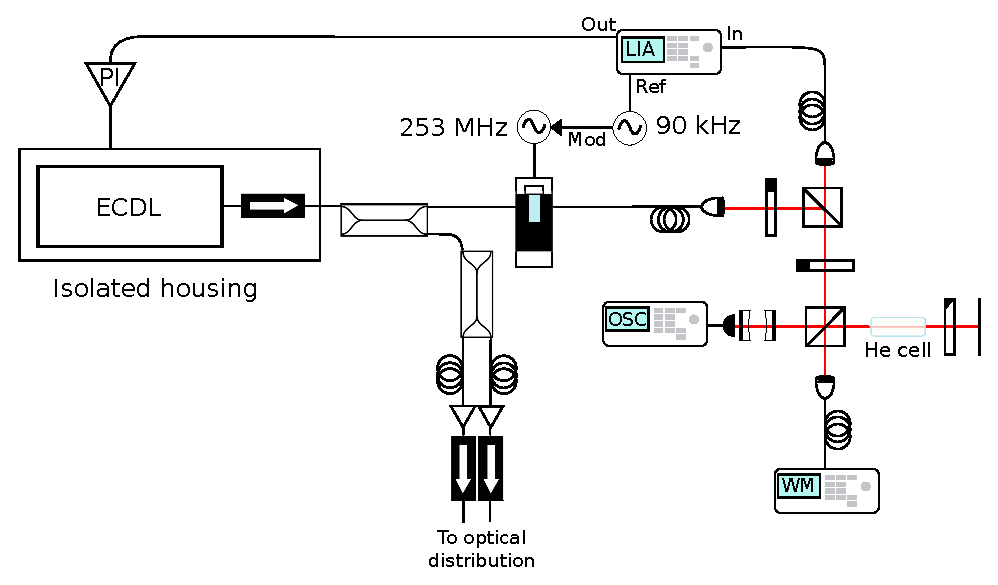
\includegraphics[width=\textwidth]{fig/apparatus/master_laser_system}
		\caption{Schematic of the generation and control system for the main cooling laser operating at 1083.331nm. \todo{double check unused channel} \todo{Put this later/after the main exp schematic}}
		\label{fig:main_laser}
	\end{figure}
	
	
	% Both machines also employ sources of 1550nm laser light, used for a crossed optical dipole trap in the lattice machine, and to implement atom-optical control elements in the BiQUIC machine. The latter techniques are mentioned here for completeness but are not discussed further as they were not used in the works in this thesis. The construction and operation of the 1550nm optics for the lattice machine are described in chapter \ref{chap:lattice}.

	% http://www.heliumbec.com/wiki/February_2017_Bake
	% https://imgur.com/a/4BxKh
	% http://www.heliumbec.com/wiki/Titanium_Sublimation


\subsection*{Optical distribution setups}

	\begin{figure}
		\centering
		\includegraphics[width=\textwidth]{fig/apparatus/lattice_cooling_optics}
		\caption{Schematic of the control and distribution system for cooling light in the lattice machine. \todo{This schematic is hard to follow, as it's hard to see what beam path is which.  Also, I'm not sure what information it conveys, given that each beam is essentially a copy of the others (in terms of the functional information this diagram shows).  You'd need to label things like AOMs, waveplates etc and probably highlight each beam in different colours or somehting for it to be useful, but I'd probably just not include it. }}
		\label{fig:lattice_cooling_optics}
	\end{figure}
	
	In each machine, a suite of AOMs are used to independently control the power and frequency of each of several specialized beams \footnote{The active component of an AOM is a crystal is driven at radio frequencies by an amplified voltage-controlled oscillator. An acoustic standing wave, constituted by phonons with frequency matched to the driving frequency, scatters light into discrete diffraction modes width momenta shifted by the phonon-lattice momentum. The action is analogoous to a diffraction grating, and described by the Kapitza-Dirac mechanism. Thus the AOM transduces electronic signals into optical frequency shifts. An analogous effect, with the role of atoms and light interchanged, is the operating principle of optical lattices.}. The first-order diffraction is usually chosen for its more efficient transmission. The pointing of the diffracted beams vary with the AOM frequency, which is a problem when the ultimate destination of the light is separated from the AOM by several meters of optical path length, after which the deflection can become significant. To circumvent this, the AOMs are set up in a double-pass `cat's-eye' configuration so the deflection in one pass is canceled by the second pass in the opposite direction.
	
	The AOM suites are supplied by light picked off from the output of the fibre amplifier by a half-waveplate and beamsplitter pair per AOM, as depicted in \ref{fig:lattice_cooling_optics}\footnote{This figure shows the AOM suite layout for the lattice machine, as I built it when working on the project. The layout for the BiQUIC machine is essentially the same.}. A quarter-wave plate placed in the optical path through the cat's-eye ensures the doubly-diffracted beams are transmitted back through the beamsplitter into the distribution optics. AOMs offer the advantage of fast switching times, but some light can leak from the AOM suite through the optical paths into the experiment. As such we used electronic shutters and an opaque enclosure to prevent this from occurring. The shutter action as well as the detuning and diffraction efficiency of the AOMs are actuated by the control software described later in this chapter. 
	


\subsection*{Spectroscopic laser}
	A light source unique to the BiQUIC machine was the tunable laser system used to generate light in the $402-430$nm range for the laser spectroscopy measurements discussed  in Chapter \ref{chap:spectroscopy}. This  was a tunable M-squared Ti:Sapphire laser system, depicted in Figure \ref{fig:tunable_laser}. Light at 1064nm from a Lighthouse Photonics Sprout module was frequency doubled by second-harmonic generation to pump an M-squared SolsTi:S titanium-sapphire laser which we operated around 800nm. The output from the SolsTi:S was doubled again in an M-squared ECD-X module to the target wavelengths. A fraction of the light is fed into a High Finesse WS-8 wavemeter. High Finesse specifies the absolute accuracy of the WS-8 at 2MHz within 2nm of a transition line, and 10MHz otherwise. We use the wavemeter to lock the tunable laser with respect to the red light, so the uncertainty is doubled in determinations of the blue frequency. We calibrated the wavemeter once every day or so with respect to the two-photon crossover transition between the $6^2P_{\frac{3}{2}} (F=4)$ and $6^2P_{\frac{3}{2}} (F=5)$ lines in a cesium vapor cell. We used saturated absorption spectroscopy to lock the red light to the Cs transition while feeding light into the wavemeter for the calibration.	A MATLAB software lock uses the wavemeter output to stabilize the laser to within 100kHz of the target wavelength, and allows automatic scans across the region of interest by automatically updating the laser set point. \todo{description of TCP lock protocol}

	\begin{figure}
		\centering
		\includegraphics[width=\textwidth]{fig/apparatus/solstis_schematic_minim}
		\caption{Schematic of the spectroscopic laser system, including calibration infrastructure. \todo{Probably need  a bit more detail in teh caption, especially as it doesn't all seem to be in teh main text.}}
		\label{fig:tunable_laser}
	\end{figure}
	
	

	We used the first diffracted mode of an AOM, driven at 189MHz, to control the beam power. The output of the AOM was fed into an optical fibre which coupled the light to the vacuum insertion optics. There, we used waveplates to set the polarization and a telescope to magnify the beam up to $\approx$2cm waist. A final lens fixed to a three-axis translation mount was used to focus and align the beam. For the measurements of the tune-out and forbidden transition wavelengths, we focused the beam to a diffraction-limited waist, about $100~\mu$m at the site of the BEC, to achieve strong interaction given the weak signals of interest \todo{double check that waist size. I think it was actually smaller, on the order of the TF radius}. For the $2\triplet P_2\rightarrow 5\triplet D$ transitions described in the bulk of Chapter \ref{chap:spectroscopy}, the beam was collimated and operated at a reduced power to mitigate power broadening and saturation of these much stronger resonances. The optical power was regulated with reference to a photodiode which sampled the beam after the fibre via a polarizing beamsplitter.

	The wavemeter logs, photodiode voltage, and transmission of light from both the 800nm and 400nm beams through two scanning Fabry-Perot cavities (SFPs) were recorded through the DAC system in order to provide diagnostics in post-processing. Part of the data analysis pipeline then automatically discarded shots where either SFP showed multiple peaks within a single free-spectral range (FSR), indicating that one of the lasers was running in am ultimode regime, or where the photodiode trace indicated a laser supply failure, or where other anomalous behavioru was detected.


	% Camera/mirror setup Reproducibility
	% issues

\section{Detection of metastable helium atoms}

	A unique diagnostic available in helium experiments is the production of helium ion-electron pairs. This process can be monitored by in-vacuum electron multipliers mounted near the trapping region. Proximity to the trap is desirable for efficient collection of the resulting particles. Aside from investigating Penning ionization itself (as mentioned earlier in this chapter), ion detection has been applied in photoassociation spectroscopy \cite{herschbach00,koelemeij04}, to monitor the onset of Bose-Einstein condensation \cite{tychkov06}, and for high-precision laser spectroscopy \cite{Rengelink18}. The ion detector in the BiQUIC machine stopped working some years ago and has not been replaced: the utility of this diagnostic is outweighed by the effort required to break vacuum for the first time in a decade or so, disassemble the chamber and surrounding optics, reassemble everything, bake the chamber, and realign all the optics. As such ion detection garners only a brief mention in section \ref{sec:DipoleAlignment}, wherein I describe an attempt to use the ion detection as an diagnostic to aid alignment of a dipole beam in the lattice machine. In an accident a year or so after I left that lab, the ceramic feed-throughs connecting the ion detector to the external electronics cracked. This broke vacuum, necessitating a rebake of the chamber, and saw the detector retired. 

	Two optical detection methods are employed in the ANU helium labs. Saturated fluorescence measurements are used to monitor the number of atoms in a trap. In this method, bright resonant light ($I\gg I_\textrm{sat}$) is applied to the atoms such that the population of the excited state saturates at 50\%. If the light is applied while the trap remains on, then while some atoms may decay to a trapped state, repeated absorption events eventually drive them out of the trap. Therefore, one expects a sharp peak and subsequent decay in the optical power re-emitted from the trap. This radiation can be captured by a lens and focused onto a photodiode, producing an analog voltage as a useful diagnostic. The difference between peak and steady-state voltage after the pulse is a direct probe of the atomic population. This technique is generally employed only as a diagnostic tool for fast readout when optimizing the alignment of cooling and trapping beams, and as such will not be discussed in further detail. The second optical interrogation technique, resonant absorprtion imaging, is only available in the upstairs laboratory. Therefore the theory, construction, and use of the absorption imaging apparatus is discussed in Chapter \ref{chap:lattice}. \todo{Maybe put maintenance after this as it's defined the sat fluro, which is better than just a diagnostic, you can make accurate number measurements with it}


\subsection*{Single-atom detection with the MCP-DLD stack}
% http://www.heliumbec.com/wiki/Detectors
	The principal detection scheme in this thesis is single-atom sensing in the far-field regime using a multichannel plate and delay-line detector combination (MCP-DLD). In some experiments, such as those conducted by the \mhe group at VU Amsterdam, the MCP itself can be used as an ion- or metastable-atom detector. In our experiments, the MCP is paired with either a phosphor screen (usually only used for diagnostic purposes) or with a delay line detector to form the MCP-DLD, which is the workhorse of most experiments conducted at ANU. A summary description is given here, and detailed explanations of the detector stack and signal processing pipeline can be found in \cite{ShinThesis, HodgmanThesis, ManningThesis}. The MCP consists of two plates, each of which feature 10$\micron$-diameter pores arranged in a square grid with 20$\micron$ between the centres of the pore openings . The plates are 80mm in diameter, with the upper surface 848mm below the BiQUIC trap centre. The freefall time-of-flight of the centre of mass of the cloud is 417ms, which means the maximum measurable horizontal velocity is about 9.5 m/s, sufficient to capture almost all of the thermal fraction for clouds below the critical temperature. The detector plates are grounded for most of the experimental sequence, and then the top plate is ramped to -2.4kV over about 2 seconds before dropping the trap. The negative voltage repels electrons from the surface of the plate which protects the detector surface from degradation and reduces the background count rate. The background rate, also called the \emph{dark count} rate, is 0.56 Hz/cm$^2$ when operating at -2.4kV, which is practically negligible for the purposes of experiments in this thesis \todo{Maybe include a figure showing this dark rate?}. 

	\todo{MCP-DLD schematic}
	When an atom strikes the surface of a pore after falling from the trap, a second-order process releases an electron with most of the  19.8eV as kinetic energy\cite{ThatPaper}. These electrons are accelerated down the pore by the strong electric field, and themselves impact the pore surface and eject more electrons, triggering an electron avalanche that amplifies each atom impact into over 10$^6$ electrons. The electron shower exits the back of the detector and is accelerated by a +300V potential towards the delay-line detector (DLD). The DLD in the BiQUIC machine consists of two coils of wire each wound in a helical pattern and arranged perpendicular to one another.  The arrival of an electron cascade causes a current pulse to travel along each wire in both directions from the point of impact. The pulses pass through a fast pre-amplifier and then through a constant-fraction discriminator which converts the analog pulses into a digital signal. Both these processes take place within a Roentdek DLATR6 which is located outside the vacuum chamber. The digital pulses are transmitted to a Roentdek TDC8HP time-digital converter (TDC) which registers the arrival time, relative to the arrival of the main trigger signal from the LabView control software, and writes these to a \verb|*d.txt| file as \verb|(channel,time)| pairs. Finally, a custom C++ script passes over the file and converts the timing data to \verb|(t,x,y)| tuples. The conversion from \verb|(channel,time)| to \verb|(t,x,y)| is performed separately, and indeed the latter usually by a different machine, so as to provide maximum CPU availability to the acquisition function.	Further details about the architecture, construction, and calibration of these detectors is found in \cite{HodgmanThesis,ManningThesis}.

	A second MCP, backed by a phosphor screen and a mirror at 45$^\circ$ to the vertical axis, is mounted on an in-vacuum translation stage below the main chamber. The mirror directs light from the phosphor screen to a CCD camera mounted outside the vacuum chamber. This detection method is not typically used for scientific purposes, but is a useful additional diagnostic when the MCP-DLD detector stack appears to be faulty. The phosphor screen does have a much larger dynamic range than the DLD, however, which makes it useful for visual spotting of subtle distortions in the BEC profile, such as used in the alignment of the spectroscopic probe beam, as described in chapter \ref{chap:spectroscopy}. 


	% % NTM [185] derivation of detector flux profiles - inc mean field 
	% % % Tychkov PhD thesis
	% % RGL [98] calibration of QE - depends on plate voltage, which in turn affects plate lifetime and rate of degradation of QE 
	% % % van Rooij PhD thesis
	% % RGL MCP flux models [94] inc BEC flux in terms of chemical potential 
	% % % van Rooij PhD thesis
	% % TKV [9,10] expanding condensate density distributions 
	% % % Y Castin, R Dum, bose-einstein condensation in time-dependent traps, Physical Review Letters 77, 1996
	% % % F Dalfovo, S Georgini, L P Pitaevskii, S stringari, theory of bose-einstein condensation in trapped gases, rev mod phys 71, april 1999
	% % SSH [38,39] condensate ballstic expansion 
	% % % Castin & Dum
	% % % K. Dieckmann, Bose-Einstein Condensation with High Atom Number in a Deep Magnetic Trap, Ph.D. thesis, University of Amsterdam (2001).
\subsection*{Atom lasers}


	% 	NB - the Einstein coefficients have a cubic dependence on frequency (See also the natural lifetime) and so optical transitions tend to exhibit spontaneous decay more quickly than the Rabi oscillations, but radio transitions (as in the fine structure states) fall much more slowly and coherent oscillations can be seen 
	% One can see that at large detunings, the oscillation frequency ncreases but the amplitude falls off like the detuning-squared, and one instead encounters the dipole potential, right?

	The most straightforward way to use an MCP-DLD to interrogate a BEC is simply to drop the atoms onto the detector. An example of this straightforward detection scheme is illustrated in Fig. \ref{fig:dropped_bec}. A drawback of this method is that the high atom fluxes in large BECs can temporarily deplete the available current carriers near the surface of the detector, resulting in a nonlinear reduction in detection efficiency known as \emph{saturation}. This means that for even moderately sized condensates, a determination of the condensate population by counting detection events or by straightforward fitting of the time-of-flight profile is impractical, and one cannot compute interesting quantities like correlation functions with meaningful accuracy. Another limitation of the trap-release method is that it is a completely destructive measurement - one cannot re-trap the cloud or only drop part of it, which slows down data acquisition for even simple purposes like determining the trapping frequencies. Atom laser methods can circumvent both of these issues. 
	\todo{Put figure closer, but keep on opposing pages}

	The basic principle of an atom laser is to transfer some portion of the condensed atoms into a state that is no longer confined by the trapping potential. This was first achieved by applying pulses of RF radiation to a magnetically trapped condensate shortly after the first realisation of BEC\cite{mewes97}. Later, a continuous-wave atom laser was demonstrated and used to perform RF spectroscopy of the cloud, revealing the symmetry-breaking action of gravity which pulls the BEC away from the minimum of the magnetic field \cite{bloch99}. Optical Raman transitions\footnote{In atom optics, \emph{Bragg} transitions, which impart a momentum transfer, are distinguished from  \emph{Raman} transitions which also induce a change in the electronic state.} can also be used as the outcoupling mechanism \cite{Hagley99} with the advantage of imparting a controllable momentum to the outcoupled atoms, but are not employed in the works in this thesis. 

	Atom lasers are so named because the trapped condensate acts as a reservoir of coherent matter waves, in analogy to lasers as a source of coherent light \cite{narashewski,glauberXX}. The first-order coherence of atom lasers is evident from the observation of interference fringes between matter-wave beams \cite{andrews97} and the higher-order coherence manifests in the many-particle correlations detected in \mhe atom lasers \cite{SomeMorePapers}. Atom lasers can also be collimated \cite{bloch99}, directed with collimated laser beams playing the analogous role of an optical waveguide \cite{Guerin06,couvert08}, and manipulated with optically-induced `mirrors' and beamsplitters \cite{Bloch01}. The potentially continuous operation of atom lasers \cite{Chikkatur02} brings the analogy with conventional lasers even closer. Atom laser physics has been studied in detail and widely deployed through the field of atom optics in the two intervening decades since their conception, including most of the works described in this thesis.
	
	% NB this Andrews paper makes some interesting points about the nature of the condensate order parameter, arrguments about whether BEC is actually coherent/hhas a phase, and the relationship between gauge symmetry breaking and particle number conservation - c.f. that recent paper about number fluctuations in a condensate, discuss in overview


	A simple explanation of the mechanism of an atom laser requires a two-level atom with magnetically trapped and untrapped states labeled $\ket{1}$ and $\ket{0}$. An RF pulse tuned to the splitting $\omega_{10}$ for a duration $t$  induces an oscillation between the two states with Rabi frequency $\Omega$. For an ensemble of $N$ atoms, the independent single-particle oscillations produce a many-body product state which evolves as \cite{mewes97}
	\begin{equation}
		(\cos(\Omega t/2)\ket{0} + \sin(\Omega t/2)\ket{1})^{\otimes N} = \sum_{n=0}^{ N}\sqrt{\frac{N!}{n!(N-n)!}}\cos(\Omega t/2)^{N-n}\sin(\Omega t/2)^n\ket{N-n,n},
	\end{equation}
	where $\ket{N-n,n}$ denotes the state with $n$ atoms coupled out of the trapped state and $N-n$ atoms remaining. The outcoupled fraction is then $\sin^2(\Omega t/2)$.
	 % Examples of the dependence of outcoupled rate with frequency can be seen in figure X. \footnote{There is the question of when the atoms actually leave the trap. In one picture, the RF pulse simply allows the atomic wavefunction to couple periodically to the decay channel corresponding to collision with the detector. So they don't actually 'leave' the trap until there's a detection event. How does one ensure we have no significant coupling to the -1 state, which would miss the detector?}

	In practise, the Zeeman splitting varies across the trap due to the inhomogeneous magnetic field, and so a narrow RF pulse would only be resonant with a section of the condensate. While offering detailed spectroscopy of the condensate, this can be circumvented by applying short RF pulses resonant with the minimum Zeeman splitting of the trap. If such pulses are sufficiently short, the Fourier broadening of the finite-duration pulse is wider than the RF width of the condensate. The typical radio-frequency width of the condensate, i.e. the difference between the resonant frequency at the centre and the edge of the condensate, is set by the chemical potential of the condensate and is typically less than 10kHz in our experiments. An example of the MCP-DLD readout from a pulsed atom laser is shown in Figure \ref{fig:pal_micro}. \todo{So what parameters do we use for our atom lasers then?  All this background is fine, but in a chapter on the experiment you need some more details of what our system actually has}
	% Therefore, an RF pulse duration of order X sec is sufficient to ensure a uniform transfer across the trap. This broadening also dominates the additional shift in Zeeman splitting by the mean-field interaction, which is of order Y kHz. 
	 % The pulses typically on the order of 100$\mu$s long, which for a typical trap splitting of order 2MHz ensures the spectrum of the pulse has a FWHM of order xMHz thanks to Fourier broadenin. 

	 \newpage
	 \begin{figure}
	 	\centering
	 	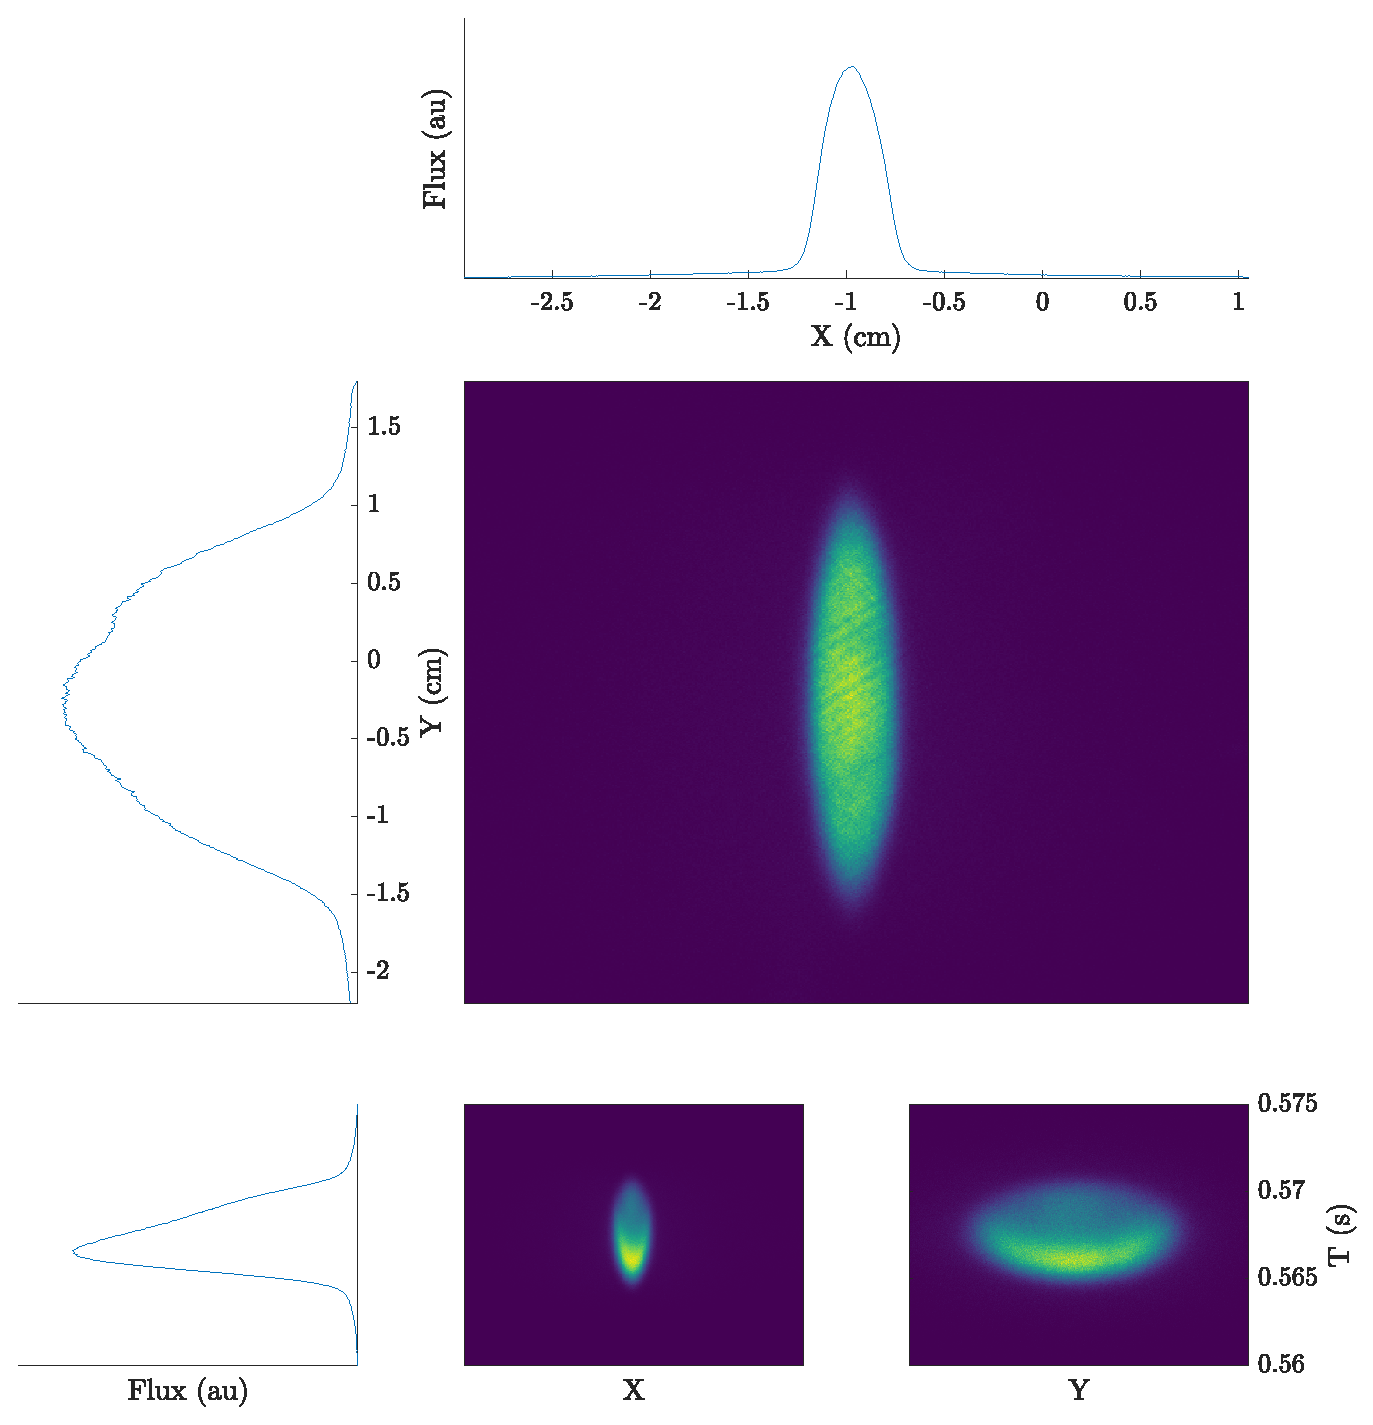
\includegraphics[width=\textwidth]{fig/apparatus/dropped_bec}
	 	\caption{MCP readout of a dropped BEC with small thermal fraction. The detector saturation is evident in the time-of-flight profiles (bottom row) as a sudden downturn in the detected flux, whereas the full BEC has a parabolic profile. The density- and space-dependence of the saturation is visible in the 2D sections (lower middle and lower right).\todo{More axis labels and ticks and such... But they're all common...}}
	 	\label{fig:dropped_bec}
	 \end{figure}

	 \newpage
	 \begin{figure}
	 	\centering
	 	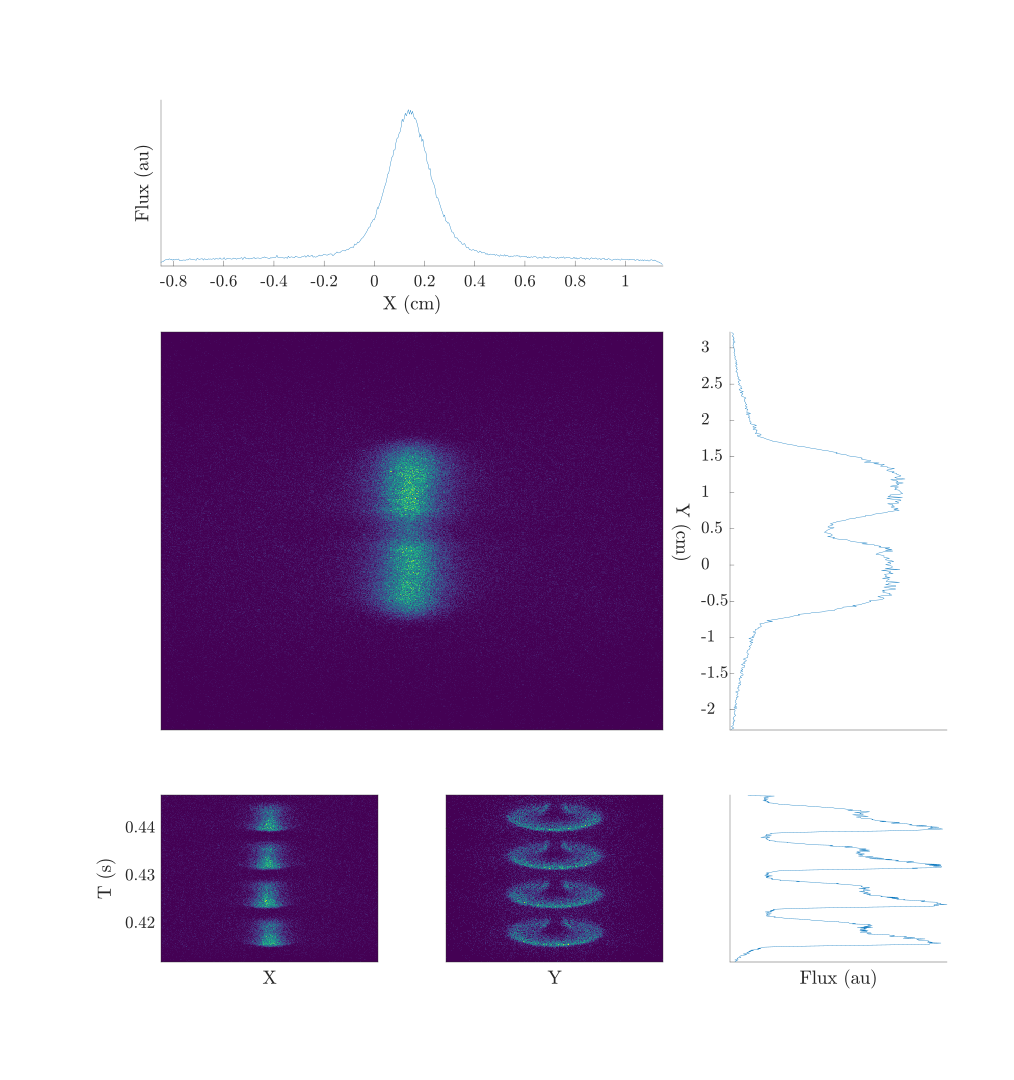
\includegraphics[width=\textwidth]{fig/apparatus/pal_MCP_micro}
	 	\caption{MCP readout of the first few pulses from a pulsed atom laser.}
	 	\label{fig:pal_micro}
	 \end{figure}
	 \todo{Without the reader knowing about atom lasers, they may think that these images look even more saturated than teh BEC!  The spatial profile certainly looks much worse.  You should at least mention that mean-field effects cause several types of distortion, and cite our earlier papers.}
	 \newpage

% PAL picture is integrated over 156 shots from 5_3d_2_3 data
% QD picture is integrated over about 1300? in tight trap fwiw from run 8

% PAL parameters; 1.6-3 MHz centering (see that ol plot) depending on trap
% pulsees 6-12 cycles
% typically sampled at 6-11 ms periods, generally limited by BEC width
% 


% tcpip interface for laser lock
% 	t = tcpip(IP, 33333, 'networkrole','server')
% 	fopen(t)
% 	fwrite(t,freq,'double')
% 	fclose(t)

% And on the other end - a loop that hammers it with queries?
% init parallel pool
% 	if workerID == 1
% 		while true
% 			try
% 				t = tcpip('localhost',33333,'networkrole','client')
% 				fopen(t)
% 				setpt = fread(t,1,'double')
% 				fclose(t)
% 				labSend(setpt,2)
% 			end
% 		end
% 	elseif workerID ==2 
% 		solstis = find_instrument();
% 		instrument_status = getResponse(solstis)

% 		write_logfile(instrment_status,metadata)
% 		% Omitting parameters for lock loop like wait times, slew rate limits, etc, various timers,

% 		if labProbe
% 			data = labReceive(1);
% 			if data != setpoint
% 				old_setpoint = setpoint;
% 				setpoint = data;
% 		red_freq = WM_query();
% 		PID_step(red_freq,setpoint,parameters)


% -> Something about communication between parallel workers?
% Ethernet link between PC and solstis driver; query returns machine state like internal photodiode readings and optomechanical actuator voltages


\section{Vacuum system integration}
	
	% Physical models often make simplifying assumptions, like ignoring air	resistance or friction, or collisions etc. Idealized models are only	solvable in certain special cases, and introducing nonlinear effects	like friction can make them mathematically intractable. This is	partially resolved by sophisticated modelling these days, but the	approximations will always remain. So when it came to studying	microscopic systems, one would like to remove the background. so that	the thing you are examining becomes not only the foreground, but the	only thing in the image, and so your signal is not obfuscated. So people	have tried to make vacuum for quite some time! Indeed this is one way	atmospheric pressure was measured - 

	While nature abhors a vacuum, experimentalists abhor a background. Ultracold atom experiments require ultra-high vacuum (UHV) conditions because collisions with a background gas can easily overcome the frail forces that hold the atoms in their traps. Our vacuum is maintained by continuous operation of several turbomolecular pumps\footnote{One of the earliest accomplishments of significant vacuum was by Lavoisier, who used pumps from the firestation to evacuate a chamber. Since then vacuum has advanced considerably, and at ultrahigh vacuum the exhaust is so dilute that one does not have the viscosity to operate pumps in the true sense. Nonetheless, the name remains.}, which are backed by roughing pumps. For the UHV chambers where BEC is created, an additional turbomolecular pump operates between the vacuum-adjacent turbo and the roughing pump.  Contamination of the vacuum chamber interior occurs from environmental sources like atmospheric pollutants or errors while handling components. When first pumping down to vacuum, contamination by water, oils, dust, or other materials can prevent achievement of good vacuum because of outgassing of volatile chemicals within the contaminant. These surface contaminants can be removed by wrapping the machine in heater tapes and insulating aluminium foil, and baking at up to 150 degrees celsius for several days. In this process one typically observes a sharp rise in pressure as the chamber heats and the contaminants volatilize, and then a decrease to a lower steady-state pressure as the contaminants cease outgassing and the remnants are evacuated. Once the pressure stabilizes, the heater tapes can be turned off, and as the apparatus cools the pressure will settle to a more preferable level. 
	% Care must be taken not to heat or cool the machine too quickly, or differences in thermal expansion between connected flanges can open leaks to atmosphere and undo much patient work. 

	% In the course of my scholarship, I extended the vacuum system of the lattice machine by constructing the LVIS, science chamber, and detector chambers. 

	Even after baking, the pressure may not be low enough to permit long-lived traps. Hydrogen leaching from the surface of the steel chamber can be significant. One method of dealing with this is by titanium sublimation. Specialized `titanium sublimation pumps' pass a large current (several amps, pulsed) through a titanium filament which sublimates titanium atoms that eventually adsorbs on the walls of the chamber. Hydrogen adsorbs to the titanium surface but not to steel, and so after some applications the pressure trends further down. Further reduction in hydrogen background can be achieved by so-called `getters', which present a highly porous surface into the vacuum and to which Hydrogen is strongly adsorbed. The chemical makeup of the background pressure can be determined using residual gas analysers (RGAs) which are essentially compact mass spectrometers. They can help diagnose whether one has an air leak or organic contaminant, and are helpful for leak hunting when paired with a bottle of helium gas, gently vented near suspect flanges.
	\todo{This paragraph is typical of a lot of this chapter - a general introduction and vague description, but no specifics as to what we actually do!  E.g. from this I'd assume we have Ti subs on both machines.  Remember that your thesis is meant to talk about what you did, and this chapter in particular should describe the machines you worked on much more than provide a general introduction to the experimental aspects of BEC machines.}

	The vacuum systems form the skeleton of both machines, which have a common structure illustrated schematically in \ref{fig:vacuum_diagram}. The placement of some of the turbomolecular pumps, faraday cups, and pressure gauges differ between the machines, but this makes no functional difference. However, the beamline of the lattice machine does not feature a deflection stage or a focus for the LVIS. Otherwise, the overall structure of the vacuum systems is the same and so only the BiQUIC machine is shown in its entirety in in Figure \ref{fig:vacuum_diagram}. \todo{put figures closer to references}

	\begin{sidewaysfigure}
		\centering
		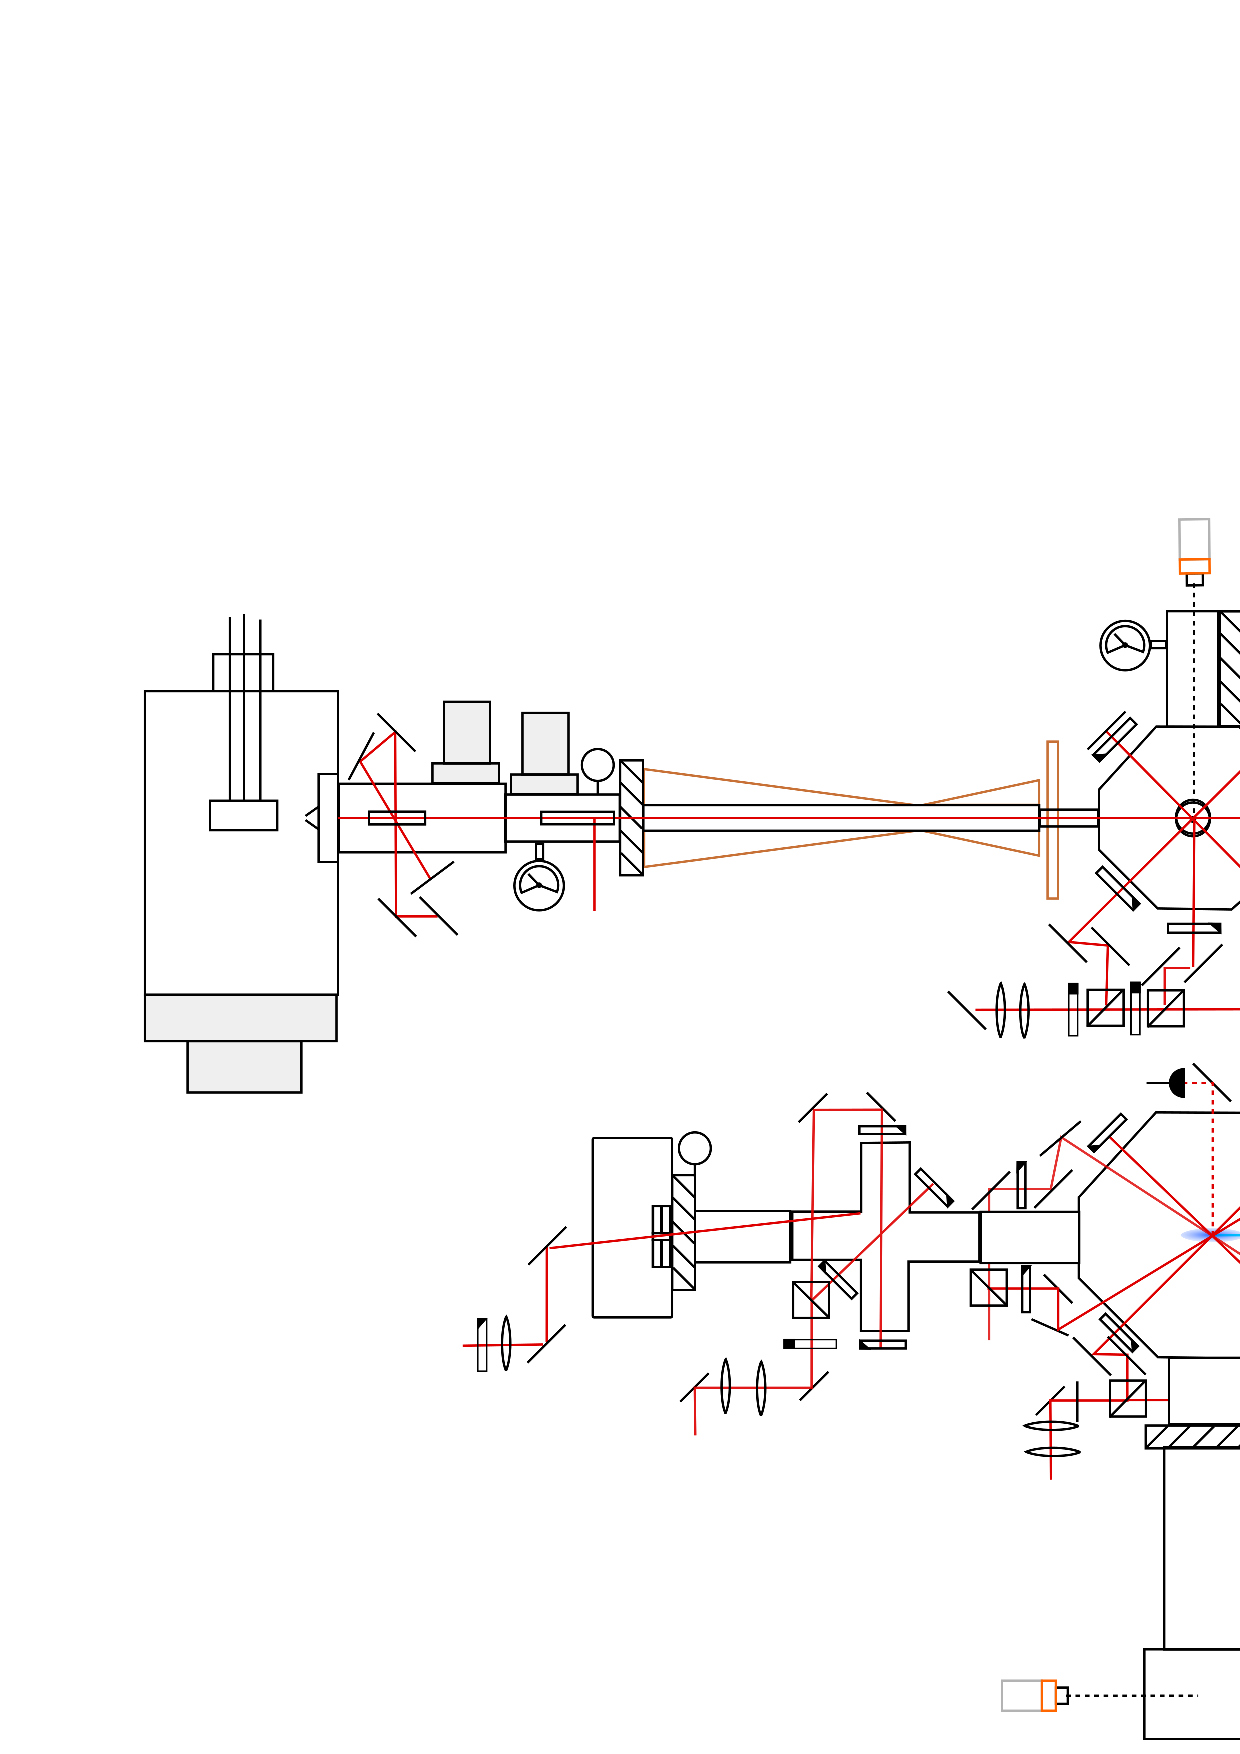
\includegraphics[width=\textwidth]{fig/apparatus/vacuum_schematic}
		\caption{Vacuum system and laser insertion optics used in the downstairs experiment \todo{These diagrams are pretty confusing... At least you need to add some labels to parts of the vacuum system, different beams etc.  A legend showing different components might help too.  In general, a diagram such as this trying to show every optical component isn't very helpful - the reader doesn't need to know about every lens and mirror in every beam path!}}
		\label{fig:vacuum_diagram}
	\end{sidewaysfigure}
	


	A major difference between the two setups is the construction of the chamber housing the final trapping stage in which BEC is achieved. the BiQUIC machine has more limited optical access and has featured the spectroscopic laser, as depicted in Figure \ref{fig:vacuum_diagram}. For comparison, the apparatus around the lattice machine's science chamber is shown and described in Chapter \ref{chap:lattice}. \todo{Probably just make this chapter exclusively about the BiQUIC machine. Differentiate the machines in the lattice chapter.}
	% This machine features 8" re-entrant windows on each face of a large Kimball chamber as well as several 3.25" (?) windows for insertion of the dipole and (eventually) lattice beams. In commparison, the science chamber of the BiQUIC machine has been running with coils built in the BiQUIC configuration for many years, but the coil housing itself precludes large windows.
	% The horizontal MOT beams in this case are limited to about 1cm diameter. The diagonal beams, in-trap cooling beams, and Bragg beams (when they are used) are inserted through small windows (1"?) protruding from the sides of the chamber.


	 %- what fraction would have sufficiently low	energy to capture, and how long would they last? 
	


\section{Data acquisition \& control}

	Control of the optical components (AOMs and shutters), coil current supplies, and RF radiation is coordinated by a central LabView program which transmits pulse sequences to the machine via National Instruments pulse cards. The cards themselves are connected to the CPU by a PCI bus, and synchronize their internal clocks at the beginning of each shot. The cards also record analog inputs such as Fabry-Perot cavity scan traces, photodiode traces, and mains voltage traces for post-processing diagnostics.

	The LabView software is old, and the absence of documentation made significant modifications impractical. A workaround was accomplished by including a command that calls a specified MATLAB subroutine (referred to as the `interface'), which is customizable to suit the purposes of a given experiment\footnote{The software developed to analyse the data from various experiments is invariably written in MATLAB. Many core capabilities are stored in the repository \url{https://github.com/HeBECANU/Core_BEC_Analysis}, and generally each project will have a unique public repository as well.	}. This subroutine can pass a \verb|.xml| file path to a LabView pulse sequence file to use in the next experimental cycle, and even modify the sequences, albeit in a limited way due to the particulars of LabView's sequence specification format. This extension allows for automatic optimization of experimental sequences, as was demonstrated in \cite{HensonML}, but obviously is of no use for mechanical tasks like beam alignment\footnote{One can dream, though.}. 
	\todo{Remove above para and fix flow}
	The interface script also writes metadata to a log file, including the POSIX timestamp, type of shot executed (e.g. \verb|calibration| or \verb|AtomLaser|), shot number, and other relevant parameters. The timestamps in this logfile can be cross-referenced with the \verb|*d.txt| files that are written by the TDC computer and with the LabView logs of analog inputs in order to match the experimental parameters with data files for post-processing purposes. The data analysis pipelines for modern experiments can be complex, and the experiments in this thesis generally comprise a handful of different diagnostics processed in parallel. The tagging of shots by timestamp cross-referencing allows separation of relevant shots for each processing subroutine. 
	An example of the detailed diagnostics produced from the logs and metadata are shown in Figure X \todo{diagnostic figure}

\subsection*{Optimizing machine performance}

	% Routine maintenance is required to keep the machine capable of producing large condensates. Despite the stabilized environment, optics are prone to wander slightly over time. The stable temperature is especially important as the cooling beams are coupled from the AOM tables to the vacuum chamber optics by free-space links. Drift in the relative position of the optics tables would therefore result in misalignment of many laser beams, and degrade performance of the machine. The conditioned air is supplied through three HEPA filters in the lab ceiling. The resulting positive pressure in an area enclosed by PVC strip walls keeps dust from entering the area on air currents. 

	If the second MOT is loading and a saturated fluorescence signal is visible, one can usually optimize all of the optical alignments on this signal, which is a factor of ten faster than the full BEC creation sequence. If this is not available, historical records of diagnostics taken at several points throughout the beamline can facilitate diagnosis of the point of failure. The most commonly employed tests are faraday cups which produce a current when impacted by \mhe atoms, as read out on a picoammeter. These current sensors are placed after the deflection stage, at the end of the Zeeman slower (with a large hole bored through it to allow the slowing beam to pass through), between the first MOT and the focus stage, and behind the second MOT chamber. In case the first MOT is not operational, a Xenics Bobcat CCD camera mounted above the chamber provides a view of the trapping region and direct visual feedback about the presence, shape, and density of the MOT. 


	% A more elegant solution could take the form of a main script that generates control pulses, absorbs the functions of the interface while monitoring the TDC output directory, and creates a direct link between log files and the \verb|d.txt| files. Unfortunately, even if LabView were able to provide all this functionality, upgrading the control software would be like moving deckchairs on the titanic. It would be more effective to replace the entire control suite, which could take several months. Given the long build times required for new experiments, during which continuous operability is essential, and that adjusting the control software is a relatively small part of the demands of operator time, this upgrade is not a high priority.  However, the control software for Staggering Grace was recently upgraded to a more readily usable and modifiable Python-based infrastructure, which will surely prove both helpful and informative for future designs.

    % \begin{figure}
    % \includegraphics[width=\textwidth]{fig/depletion/partition_QD_files_01_shot_counts_combine}
    % \label{fig:qd-count_by_type}
    % \caption
    % \title
    % \end{figure}





   
 %   Notes on new BEC paper
	% We report the realisation of Bose-Einstein condensation (BEC) of metastable helium atoms using an in-vacuum coil magnetic trap and an optical dipole trap. A novel quadrupole-Ioffe configuration (QUIC) magnetic trap made from in-vacuum hollow copper tubes provides fast switching times while generating traps with a 10G bias without compromising optical access. The bias enables in-trap 1D doppler cooling to be used, which is the only cooling stage between the magneto-optic trap (MOT) and the optical dipole trap. This allows direct transfer to the dipole trap without the need for any additional evaporative cooling in the magnetic trap. The entire experimental sequence takes 3.5 seconds, with essentially pure BECs observed with ∼ 1e6 atoms after evaporative cooling in the crossed dipole trap.

	% Get Herwig Ott paper [7] for thesis ref

	% Collim 67Isat, -5Gamma
	% 5W fibre amp for cooling beam
	% ZS 92Isat -160Gamma
	% MOT1 87Isat horz 110ISat vert -22Gamma detuning
	% 1.5mm hole in chamber
	% <3e-11 mTorr
	% push 110Isat 3.5Gamma for low-velocity intense source LVIS
	% Flux into 2nd MOT is 9e8 atoms/sec using faraday cup and picoammeter
	% Second MOT gradient 4.4G/cm (in weak or strong axes?)
	% -33Gamma and 140, 37 Isat
	% 1.7e8 atoms loaded at 2.5mK in 1 second, as measured using saturated fluro on an InGaAs PD [26]
	% 451mm fall to detector
	% 	DLD not operational yet so measure the current pulses on the plates frmo the charge depletion when atoms impact the plates. Fast amplifier and a discriminator then recorded using a digital counter to extract 1D tof distribution.
	% MOT compression - ramps to 1.42G/cm in 10ms while linearly ramping lasers to -0.4Gamma and decreasing intensity by a hundredfold, then switching off and the +1s remain trapped
	% Then compress the mag trap to 16.6G/cm in 100\mu s, and ramp the bias up in 100ms to provide a 10G bias in the QUIC trap. Has radial 89Hz and 57Hz z freqs. Have 5.3e7 atoms at 0.44mK. Measured using absorption imaging along the x axis using an InGaAs CCd. Flipper mirrors allow operation on the MOT axis but mean imaging not available during MOT.
	% 1D Doppler cooling [tychkov paper 25], with .01Isat and sigma+ polz directed vertically down along the bias direction. Detuned -Gamma/2.  After 500mss have 4.9e7 atoms at 83\mu K. Ready for dipole transfer.
	% 100kHz seed at 1550nm feeds a 30W amplifier, but produces 6W (y axis) and 1W (10degrees from X, in the XY plane) after AOM and fibre coupling losses. Waists are 73 and 55 micron respectively, crossing the centre of the biased trap, 6mm above the centre of the horz coils
	% Trap freqs 1.1,1.2,1.7 kHz and 150muK deep
	% Doppler cooling seems more effective with dipole beams on as it works at better at high density [25 tychkov] - indeed improving final atom number by some 50%. So they are ramped on over 100ms prior to doppler cooling
	% QUIC trap linearly relazed to an unbiased trap with 1.1G/cm gradient and then switched off with a FET. Additional square coil is switched on to create a uniform 1.6G field pointing in z direction. Turned on before the QUIC rampdown starts. Eventually found that the earth's field was sufficient to maintain the quantiation axis and suppress Penning ionization, so is switched off after 700ms in ODT. Measure 5e6 atoms at 13.5muK, 0.5 PSD
	% Trap depth reduced by exponential rampdown of power over 1 sec. 

	% Can extract mu via R_tf ^2 / 2t_tof ^2, and so from TF picture get N_0 = (2mu)^{5/2}/(15\sqrt{m}\hbar\bar{\omega}^3 a).
	% Cross T*_c at 6\mu K with 3e6 atoms, down to 80% BEC with 1e6 atoms


	% is that supposed to be a dot product?. The dipole potential is proportional to the intensity and the real part of the polz, which descrives the in-phase component of hte oscillation. The force is given by the gradient of this potential. The absorption from the driving field (and reimission in steady-state) is 
	% $P_{abs} = \langle\dot{\textbf{p}}\textbf{E}\rangle = \frac{\omega}{\varepsilon_0 c}Im(\alpha) I$. The scattering rate is therefore $P/\hbar\omega$. The Lorentz oscillator considers an electron with an SHO-like elastic binding to a fixed nucleus, with natural freq $\omega_0$ and a damping rate $\Gamma$. The resulting DE 
	% $x''+\Gamma_{\omega}x'+\omega_0^2x = -e E(t)/m_e$ includes the natural decay rate 
	% $\Gamma_{\omega} = e^2\omega^2/6\pi\varepsilon_0 m_e c^3$, which gives a solution for 
	% $\alpha=\frac{e^2}{m_e}\frac{1}{\omega_0^2-\omega^2-i\omega\Gamma_\omega}$. 

	% In the limit of large detunings, negligible saturation, and in the rotating wave approx, one finds
	% $$
	% U_{dip}(r) = \frac{3\pi c^2}{2\omega_0^3}\frac{\Gamma}{\Delta}I(r),
	% $$
	% $$
	% \Gamma_{sc} = \frac{3\pi c^2}{2\hbar\omega_0^3}\left(\frac{\Gamma}{\Delta}\right)^2I(r),
	% $$
	% Yielding the useful relation $\hbar\Gamma_{sc} = \Gamma U_{dip}/\Delta$, indicating two important principles: The scaling with intensity and detuning, and the importance of the sign of the detuning.

	% In multilevel atoms, one can extend the argument to other higher-lying states and compute the polarizability farther from several resonances, which leads towards tuneout wavelenghts...


	% This semiclassical model captures the absorption and stimulated emission of light from an electromagnetic field, but does not explain spontaneous emission. A fully quantum-mechanical treatment of the system (such as the Jayne-Cummings model) will also fail in this respect. The mechanism of spontaneous emission requires the theory of QED for a full explanation, wherein vacuum fluctuations produce short-lived virtual particles - including photons - which occasionally have the right wavelength to stimulate emission from atoms. We will not explore this detail here, but remain satisfied with the natural lifetime 
	
	


	% The interaction of an electric field with an atom induces a dipole $-e\textbf{r} - \varepsilon_0 \chi_a \textbf{E}$, where $\varepsilon_0\chi_a$ is the scalar polarizability (there are higher terms, as treated later). The interaction energy is 
	% $U=-\frac{1}{2}\varepsilon_0\chi_aE^2$ - by reference to the work above. The force follows from $F = -\nabla U$. A radiation field with frequency $z$ propagating along the $z$ direction gives rise to a force, averaged over timescales much larger than $1/\omega$, which can be written in terms of the Bloch components
	% $$
	% \bar{F}_z = \frac{-\hbar\Omega}{2 E_0}(u\frac{\partial E_0}{\partial z} - v k) = F_{dipole}+F){scatt},
	% $$

	% where $k$ is the wavenumber of the light, finally giving rise to 
	% $$
	% F_{scatt} = \hbar k\frac{\Gamma}{2}\frac{\Omega^2/2}{\delta^2+\Omega^2/2+\Gamma^2/4}
	% $$

	% $$
	% F_{dipole} = -\frac{\hbar\delta}{2}\frac{\Omega^2}{\delta^2+\Omega^2/2+\Gamma^2/4}\frac{\partial\Omega}{\partial z},
	% $$
	% The latter goes to zero on resonance ($\delta=0$). This argument applies for all three spatial dimensions and so one arrives at $U_{dipole} \approx \frac{\hbar^2\Omega}{4\delta}$, once again. One can also arrive at a similar expression for the radiative force by considering a simple model of photons with wavenumber $k$ being absorbed and emitted at a rate $\Gamma$, where the re-emission process imparts a zero impulse on average, but is limited in temperature.
	% from \cite{Grimm00}


	% An experimentalist is occasionally required to negotiate the geometry of trapping fields, laser beams, and polarization vectors in order to correctly configure optics. A method follows.

	% For an electric field propagating with a wavevector $\vec{k}$ in the lab frame across an atom in a magnetic field $\vec{B}=B\hat{\vec{B}}$...
	% 	The electric field of a purely polarized light ray at a point in space can be expressed as

	% $$
	% \textbf{E}(t)=\begin{bmatrix}
	% E_x(t)\\
	% E_y(t)\\
	% E_z(t)
	% \end{bmatrix}
	% $$

	% If we fix the axis of propagation to be $\hat{z}$, then we can write

	% $$
	% \textbf{E}(t)=\begin{bmatrix}
	% E_{x0} e^{i(kz-\omega t -\phi_x)}\\
	% E_{y0} e^{i(kz-\omega t -\phi_y)}\\
	% 0
	% \end{bmatrix}
	% $$

	% We can then define the Jones vector $\textbf{J}_0 = \left(E_{x0}e^{i\phi_x},E_{y0}e^{i\phi_y}\right)^T$, so $\textbf{E}(t) = \textbf{J}e^{i(kz-\omega t)}$.

	% In this frame, the amplitudes of horizontal and  vertical polarization are $E_{x0}$ and $E_{y0}$ respectively. Therefore, diagonal polarization is a linear combination of both these components, and circularly polarized light is a linear combination with an imaginary coefficient. 
	% A shortcoming of the Jones calculus is that it is only applicable to light which is completely polarized (that is, for some basis it can be written as $\textbf{E} = (E_0,0)$). This is not true for a beam whose polarization varies, or where there are power fluctuations in one of the axes, etc. There should be a single motivating example somewhere, but these are some examples. If this assumption is not permitted - by which measurement would you tell the difference? - then we must move to the Mueller calculus. %Determining purity of polz empirically


	% When working with two-level systems it is convenient to introduce the density matrix $\rho$. The assumption that the system must always be in \emph{some} state can be written as the normalization condition
	% \begin{align}
	% 	1&=\sum_i |\braket{\phi_i}{\psi}|^2\\
	% 	 &= \sum_i \braket{\phi_i}{\psi}\braket{\psi}{\phi_1}\\
	% 	 &= \textrm{Tr} \rho,
	% \end{align}
	% where the Trace operation is defined by $\textrm{Tr}(\ket{a}\bra{b})=\braket{b}{a}$. 
	% The density matrix permits a statistical approach to ensembles of conditional states, which will be useful in later chapters, and unifies the treatment of the important features of atom-light interactions, which is the subjects of the rest of this section. \footnote{The density matrix formalism also allows for treatment of statistical mixtures of quantum states on equal footing with so-called `pure' states which are certain to be in some state $\ket{\psi}$. While the normalization condition is guaranteed to hold for any $\rho = \sum_i p_i\hat{rho}_i$, there is no such way to write mixtures in the form $\ket{\Psi}=\sum_i\ket{\psi_i}$ without violating the assumption of conservation of probability. Indeed, pure states, defined by $\textrm{Tr}(\rho^2)=1$, are quite exceptional: They are a set of zero measure in the set of all positive semidefinite Hermitian operators with unit trace.}. When expressing the state  in terms of the energy eigenbasis $\{\ket{n}\}$, the diagonal elements $\rho_{ii}\in\mathbb{R}$ are the \emph{populations} of the $i^{\text{th}}$ eigenstate and the off-diagonal \emph{coherences} $\rho_{ij}=\rho_{ij}^{*}$ capture the utility of the quantum state for interferometric purposes\footnote{In what sense? c.f. Ramsey interferometry}. 

	% By working in a rotating reference frame via the change of basis\footnote{This change of basis induces a change to the coefficients $c_n=\exp((-1)^n \delta t/2)$} $\hat{U} = \textrm{diag}(e^{i\delta t/2},e^{-i\delta t/2})$, in terms of the detuning $\delta=\omega-\omega_0$, one can write the Hamiltonian in the convenient form \cite{FootAtomic}

	% \begin{equation}
	% 	\hat{H} = \frac{\hbar}{2}\begin{pmatrix}\delta&\Omega\\
	% 											\Omega&-\delta\end{pmatrix},
	% \end{equation}
	% which has eigenvalues $E'_\pm = \pm \sqrt{\delta^2+\Omega^2}/2$, retaining the bare splitting $\delta$ between levels when $\Omega=0$. In the presence of an oscillating field which drives an allowed transition, i.e. when $\Omega>0$, the energy of the \emph{dressed state} of the atom are shifted with respect to their unperturbed values

	% %  For now we will simply note that the average of a set of measurements of the quantity $Q$ on an identically-prepared system can be calculated via the expectation value of the corresponding operator $\hat{Q}$,
	% % \begin{align}
	% % 	\langle Q\rangle &=  \bra{\psi} \hat{Q}\ket{\psi}\\
	% % 	&= \textrm{Tr}(\hat{Q}\rho),
	% % \end{align}
	% % and that the time-dependence of the expected value follows from Ehrenfest's theorem
	% % \begin{equation}
	% % 	i\hbar \frac{\partial}{\partial t}\langle Q\rangle = [\hat{H},\hat{Q}],
	% % \end{equation}
	% % which holds equally well for the density matrix, providing the von Neumann equation $\dot{\rho} = i[\rho,\hat{H}]/\hbar$.
	
	% Let us concern ourselves with a further simplified picture of the atom as well: Indeed, we model the atom with the simplest nontrivial quantum system, one with only two distinguishable states. A two-level system permits convenient expression of the entire density matrix
	% \begin{equation}
	% 	\hat{rho} = \begin{pmatrix}
	% 		\rho_{11}&\rho_{12}\\
	% 		\rho_{21}&\rho_{22},
	% 	\end{pmatrix}
	% \end{equation}




	% The wavefunction $\Psi$ of an electron of mass $m_e$ moving in a central potential $V(r)$ can be written in terms of the bound eigenfunctions (also called \emph{orbitals}) of the Schr\"{o}dinger equation
	% \begin{equation}
	% 	\left(\frac{-\hbar^2}{2m_e}\nabla^2 + V(r)\right)\psi_{nlm} = E_n\psi_{nlm},
	% \end{equation}

	% which have the form


	% On the optical Bloch equations;
	% Starting from the density matrix, 
	% $$
	% \begin{bmatrix}
	% \rho_{11} & \rho_{12}\\
	% \rho_{21} & \rho_{22}
	% \end{bmatrix} = \ket{\Psi}\bra{\Psi},
	% $$
	% We make the unitary transformation into a rotating frame by $U=\exp(diag(-i\delta t/2,i\delta t/2))$, which is a gauge transformation such that the zero energy is exactly between the upper and lower states, 
	% $\delta=\omega-\-\omega_0$. This looks like a transformation $U = \exp(-i\sigma_z t)$ where $\sigma_z$ is the first of the Pauli matrices which generate the unitary group of dimension 2. In the rotating frame one then has the Bloch vector defined by 
	% $R_i = Tr(\rho\sigma_i)$. One can then transform the differential equations for $c_i$ into the rotating basis and obtain the time evolution of the system which can be conveniently written in the form $\dot{R} = R\times W$ where $R$ is the Bloch vector and $W=\Omega\hat{e}_1+\delta\hat{e}_3$.  
	% One can include damping by adding a decay term of the form $\dot{\rho}_{22} =-\Gamma\rho_{22} + \Omega \sigma_y/2$, which recovers the exponential decay of the excited state in the absence of a driving field. We finally have the optical bloch equations, which (may) still be expressible in a neat vector form?
	% $$
	% \dot{u} = \delta v - \Gamma u/2\\
	% \dot{v} = -\delta u + \Omega w - \Gamma v/2\\
	% \dot{w} = -\Omega v - \Gamma(w-1)
	% $$, 
	% which capture the population dynamics of a two-level atom coupled to a radiation field near resonance with significant spontaneous decay. A similar procedure can be extended to many-level atoms (one-two-many quote), and is employed in chapter X appendix Y to predict the SNR of interrogating the forbidden transition.

	% In the rotating frame one can write the Schrodinger equation in terms of the amplitudes in the rotating frame 
	% $$
	% i\frac{d}{dt}(\tilde{c}_1,\tilde{c}_2) = \begin{bmatrix}\delta/2&\Omega/s\\\Omega/2&-\delta/2\end{bmatrix}(\tilde{c}_1,\tilde{c}_2),
	% $$

	% which has eigenvales $\lambda = \pm(\delta^2+\omega^2)^{1/2}/2$ - which reproduces the raw splitting $\delta$ in the absence of a field. When $\Omega>0$ - see Cohen-Tannoudji for a deeper treatment of this dressed state picture. When the detuning is much larger than the rabi frequency then one gets $\lambda\approx\pm(\delta/2 + \Omega^2/4\delta)$, which is the bare detuning with a light shift given by the second term. The sign of the shift is given by the detuning. This light shift, or AC stark shift, is what underpins the working of the dipole force. 
	% Dipole beams are widely used in biophysical contexts for manipulation of DNA, proteins, and even entire bacteria. See Ashkin 1997 or Lang and Bloch 2003?
	% $\varepsilon$
	
	% Radiation pressure traps afew K deep, can cool to some 10s of $\mu$ K
	% Typical dipole traps less than a mK deep!
	


	% RGL Theory of AC stark shift for polz; [107-108] theory, latter Lorentz oscillator model, treats as SHO basically? Which is damped by emission of radiation - gives  second order ODE which can be solved. Good for weak driving. 
	% Of course, corrections are needed when other transitions are important, i.e. when fairly close to a strong line
	% RGL [109] second order perturbation sums over all possible final states. 
	% % Sobel'man I, introduction to the theory of atomic spectral Pergamon press 1972
	% show that the polzability can be written in the familiar alpha eqn 
	% % A Derevianko, H katori, physics of optical lattice clocks, rev mod phys 83, 2011
	% % J R P Angel, P G H sandars, the hyperfine structure STark effect, proc roy. soc. a, 305 1968		
% % \hypertarget{optical-lattice}{%
% \section{Optical lattice}\label{optical-lattice}}
% \chapter{Towards an optical lattice for quantum simulation}
% \section{Quantum $\cap$ Complexity}\label{sec:lat-introduction}
% \section{Optical lattices}\label{lat-history}
% % \subsection{Helium's promise}\label{lat-helium}
% \section{Lattice construction at ANU}\label{ssec:lat-motivation}
% \section*{Future work}\label{lat-futurework}


\chapter{Towards an optical lattice trap for helium}
   \label{chap:lattice}
   \todo{Find the balance between digression (for motivation's sake) and cohesion with the Overview chapter}
   \todo{Heavy edits on motivation}
   \todo{Double-well system example? Wannier function and ED code?}
   \todo{Incorporate optical diagrams properly}
   \todo{Description of dipole optics}
   \todo{Diagram and samples of absorption imaging}
   \todo{Discussion and pictures of build}
   \todo{Use the line `In this section we deal with the nuts and bolts (literally) of assembling a cold-atom machine'}
   \todo{Tales of dipole alignment; abs img 'comet', the 'cleft' and prior misadventures, dipole beam profiling, reason lattice beam not locked}
   \todo{More to say/cite about correlation functions and the many body problem, callback to quasiparticles/emergent stuff...}

\section{Motivation}
% keep to 1 page
	A keystone in the endeavour of physical science is the ability to foresee physical properties of substances that do not yet exist.
	The art and science of materials engineering dates back at least as far as early ceramic or metallurgical work.
	As humankind has developed more sophsticated and reliable understanding of the mechanisms underlying physical properties, so too has the design of new materials become guided more by principle and prediction than random combinatorial search.
	In the solid-state domain, where large numbers of constituent particles are correlated by non-negligible interactions, this project is particularly challenging because analytical models may be conceivable but analytically intractable, and the typical recourse to numerical computing is prohibited by the onerous demands on computer memory or runtime or both.
	Parallel to the trend of increasing precision and scale of physical models is the widening perspective of theoretical physics founded on the premise that \emph{information is physical}.
	Long has it been said that the workings of nature conform to mathematical language; the welcome infiltration of computer science into physical science now offers bridges from the physical to the computational.
	The concept of \emph{abstraction} is central in computer science and formalizes the notion of substrate-independence.
	This is what allows the realization of universal computing in the Von Neumann architecture, instantiated in enormous variety from the prototypical Colossus and ENIAC to the Summit supercomputer and Arduino microcontrollers.
	Abstracting the notion of abstraction away from computer science and into physics provides grounds for the growing field of \emph{quantum simulators}: If you care about the physics, you care about the Hamiltonian, not the objects that the summation indices refer to.
	The hope, then, is that one can build systems that are governed by  particular (or, perhaps, arbitrary) equations of motion such that your experimental system can generate useful data to constrain the search for new material design at a more affordable rate than conventional computing, when measured in some combination of time, energy, or some other convenient currency.
	One flourishing branch of this field of inquiry is the use of \emph{optical lattices} to synthesize artificial crystals, scaled up some 10,000 times and many orders of magnitude colder than conventional solids.
	The ultracold atoms in such systems then play the role of electrons bound in the ion lattice of solid systems.
	In some of these devices, the sophstication and subtlety of the experiments surpasses direct simulations of solid-state models and encroaches on the central questions about emergent complexity, fundamental particle physics and the arrow of time.
	For all their dizzying capabilities, optical lattices have to date relied upon only coarse measurements of momentum-space information, precluding access to detailed dynamical information such as particle currents and aspects of quasiparticle formation.
	Ultracold metastable helium thus offers a dramatic extension of the questions one can ask of optical lattice simulators.
	This chapter details the early development and ongoing efforts at the ANU \mhe group towards realizing this potential.


\begin{adjustwidth}{1.5cm}{0cm}
\begin{flushright}
\emph{``It might be noted here, for the benefit of those interested in exact solutions, \\
that there is an alternative formulation of the many-body problem:\\
How many bodies are required before we have a problem? \\
G.	E.	Brown points out that this can be answered by a look at history.	\\
In eighteenth-century Newtonian mechanics, the three-body problem was insoluble.	\\
With the birth of general relativity and quantum electrodynamics in 1930,\\ the two- and one-body problems became insoluble. And within modern\\
 quantum field theory, the problem of zero bodies (vacuum) is insoluble.\\
So, if we are out after exact solutions, no bodies at all is already too many!"}\\
 - Richard Mattuck\footnote{R. Mattuck, \emph{A Guide to Feynman Diagrams in the Many-Body Problem}, Dover Books on Physics (1992)}
\end{flushright}
\end{adjustwidth}

\section{The many-body problem}
\subsubsection*{There's always a bigger Hilbert space}

% 	it from bit

% 	The prospect of simulating one quantum system by another goes back at least as far as Feynman \cite{Feynman82}, who noted in the 80s that the rapid growth of the Hilbert space with the number of objects $N$ presented a serious obstacle to computational physics.
% 	More concretely, given two quantum systems $A$ and $B$ with $d_A$ and $d_B$ degrees of freedom each, the natural way to represent the composite of the two systems is the tensor product $\mathcal{H}_C$ of their respective Hilbert spaces $\mathcal{H}_A$ and $\mathcal{H}_B$, whose basis can be written as
% 	\begin{equation}
% 		\{\ket{e_C}\} = \{\ket{e_A e_B}\} = \{\ket{a_A}\otimes\ket{e_C}\},
% 	\end{equation}
% 	where the dimension of the composite system $d_C = |\{\ket{e}\}| = d_A d_B$; a simple illustration of the resource challenge is that a system of $N$ two-level systems thus has a total dimension $2^N$.
% 	A pure state can be represented as a vector with $2^N-1$ coefficients (the asymptotically trivial reduction by 1 owing to the normalization of the wavefunction), but a general mixed state must be encoded in a density matrix while tracking $2^{2N-1}-1$  coefficients\footnote{While the density matrix has $2^N\times2^N$ entries, the normalization condition and symmetry properties reduce this slightly, but this is no general recipe for ameliorating the many-body problem.}.
% 	The Hamiltonian, if similarly stored as a full matrix, has comparable memory requirements.
% 	If the complex coefficients are to be represented by pairs of floating-point number with single precision (for 8 bytes per coefficient), the memory of a consumer-grade laptop is exhausted by the state vector of 16 two-level systems; the density matrix and hamiltoniane exceed available memory for even smaller systems.
	

% 	Fortunately it is not always necessary to store the full state vector, density matrix, or Hamiltonian in memory.
% 	For the latter, a sparse representation suffices as most systems of interest exhibit local coupling only, and so most coupling constants are zero.
% 	However, matrix diagonalization algorithms exploit tradeoffs between memory use and compute depth, which one must confront when dealing with time-dependent problems or parametrized Hamiltonians.
% 	The memory requirements for the state vector can also be reduced for purposes of simulations by using inventive representations.
% 	A full review of numerical techniques is far beyond the scope of this thesis, but we will note that exact diagonalization \cite{Zhang10} is complemented by an expanding suite of techniques including matrix product states \cite{Schollwoeck11} employing the density-matrix renormalization group iterative method \cite{Dechiara08}, the Multiscale entanglement renormalization ansatz \cite{}, more general tensor-network representations, quantum Monte Carlo simulations, and emerging techniques using artificial neural network representations of many-body states \cite{}.
	

% 	Common classes of computational approach; ground-state solving (variational algorithms), time evolution, ...?
% 	Physical insight -> dimensionality reduction; where these not obvious, neural networks can do well...
% 	% -> Sometimes many-body systems are tractable because one can reduce the degrees of freedom; eg meanfield, thermodynamics in the extreme case...
% 	occasionally one is limited by insoluble equations or intractable integrals, but where exact solutions are absent sometimes asymptotically-correct approximations do OK...
% 	occasionally we are limited by ingenuity, but in general we are compression-limited in dealing with strongly-correlated systems
% 	% state of the art of QMC - people have done 3D bose hubbard right, and done exceptionally well.
	

% 	Quantum-native platforms offer a route by which to circumvent some of these issues; clearly Nature has no trouble evolving the state of some $\mathcal{O}(10^23)$ spins in solid materials; if one encodes the physics of interest \emph{directly} into another quantum system, then the space (memory) requirements of simulating quantum systems is obviated.
% 	This does present another challenge, which is the means of instantiating the state and the means of implementing state evolution.
% 	Among a wide class of specialized algorithms with less obvious physical counterparts, such as prime factoring or graph partitioning, quantum simulation is within the purview of universal quantum computers.
% 	A fairly direct translation of classical techniques to digital quantum computers is \emph{Trotterization}, whereby one approximates the time evolution of the state vector
% 	\begin{equation}
% 		\ket{\psi(t)} = \hat{U}(t)\ket{\psi(0)} = \exp(-i\hat{H}t/\hbar)\ket{\psi(0)}
% 	\end{equation}
% 	by breaking the unitary evolution into iterative application of an approximate unitary operator with time step $\Delta t$ as
% 	\begin{equation}
% 		U_{k} = \exp(-i\hat{H}k\Delta t/\hbar).
% 	\end{equation}
% 	More modern and quantum-native approaches include qubitization....
% 	Quantum simulation basically quantum-state monte carlo for some approaches...

% 	As of the time of writing this dissertation, the largest digital quantum computers have around 50 qubits, and are not able to implement fault tolerant quantum computation at a physically meaningful scale.
% 	While the early results claiming a quantum advantage have made it to press, the public sphere has not been informed of any simulations of physical systems that are definitively beyond the reach of modern or near-term classical computers.
% 	Important milestones have been reached along the way in trapped ions \cite{} and superconducting cirtuits \cite{}
% % various forms of isolated quantum systems...
% 	such that information doesn't leak in (unless you're building a sensor, you want your state to be independent of what's going on around it, other than your controlled inputs)
% % 	Optical Nicely isolated, but (??) roadblocks?
% % 		% Garanovich et al, Light propagation and localization in modulated photonic lattices and waveguides, physics reports 518, 2012
% % 		% Recent xanadu paper?
% % 		% Boson sampling result
% % 	Trapped ion  fast and high fidelity but envt decoherence is a challenge:
% % 		% Blatt et al, Quantum simulation with trapped ions, nature physics 8, 2012
% % 		lanyon, universal digial sim https://science.sciencemag.org/content/334/6052/57
% % 	Superconductors fast and high fidelity but envt decoherencfe is a challenge:
% % 		% Houck et al, on-chip quantum simulation with superconducting circuits, nature pysics 8, 2012

% 	An important counterpart to universal digital quantum simulation is \emph{analogue} simulation\footnote{So called as they rely on the prinicple of controlling physical systems analogous to the systems of interest, not because of the use of analog signals as in the digital/analog dichotomy.}.
% 	The closest analogy in classical computing is the ASIC, or application-specific integrated circuit: analogue simulators are direct and dedicated simulations of a specified family of Hamiltonians for exploration of that system in particular.
% 	The prominent physical platforms for such simulation are in trapped ions \cite{}, others \cite{}, and optical lattices, which are the focus of this chapter.
% 	While schemes have been proposed for universal quantum computing with neutral atoms in optical lattices \cite{Brennen99,Henriet20}, this potential is still some way off \cite{Markov00}.
% 	Meanwhile, analog simulation in optical lattices is flourishing.
% 	For the second time, we will note that `any attempt to produce a comprehensive review is out of date by the time it is published' and, in the below, survey some pivotal results in order to clarify the specific contributions that metastable helium atoms could make to the suite of capabilities in optical lattices.

% % 	% ah yes; QMC and the sign problem...
% % 	% 	that gravity paper? Sign problem is topological? But so far only a barrier to 'general' solutions?
% % 	% 	\cite{Ringel17} %https://advances.sciencemag.org/content/3/9/e1701758, https://advances.sciencemag.org/content/6/33/eabb8341.abstract,		https://journals.aps.org/prresearch/abstract/10.1103/PhysRevResearch.2.032060

% % high energy phys models, exotic states of matter; forecast to quantum-active matter with native cellular compute...
% 	insertion of 'agents' directly into a synthetic physical envt

\subsubsection{Quantum simulation with optical lattices}

	% Optical lattices found their use in cold-atom science for spectroscopic, interferometric, and atom-optical applications before they burst onto the scene as quantum simulators.
	% However, that rich history is beyond our scope here.
	% The first headline-grabbing experiment was the achievement of the Mott insulating state\footnote{A hallmark of the Mott insulator is the suppression of number fluctuations at each lattice site (i.e.
	% \emph{number squeezing}), which was first observed a year prior in \cite{Orzel01}.
	% However, the later result was the first to eliminate number fluctuations in 3D - see \cite{Morsch06} for discussion.} in a lattice filled with ultracold bosonic atoms \cite{Greiner02}, realizing the proposition by Dieter Jaksch \emph{et al.} from three years prior \cite{Jaksch98}.
	%  The subsequent few years saw an explosion of foundational research and technical development, summarized in the reviews \cite{Morsch06,Bloch08}, and the following decade heralded many major advances in quantum simulation \cite{Bloch12,Gross17}.
	% Theoretical foundations of the myriad models realized in lattices, and their context in a more general condensed-matter setting, are discussed in \cite{LewensteinLattices, lewenstein07}.

	% The central principle of an optical lattice is the careful deployment of the optical dipole force \cite{Grimm00} to `paint' a potential energy landscape with a persistent periodic structure.
	% A stable laser is reflected back on itself, creating a standing.
	% Atoms in this optical field thus subject to a periodic potential along the axis of propagation of the laser.
	% For a red-detuned beam, the potential energy is minimized at the intensity maxima, providing transverse confinement as inherited by the structure of the beam.
	% If the lasers are in the TEM(0,0) mode, the Gaussian profile provides an approximately harmonic confinement when the kinetic temperature is small.
	% At ultralow temperatures, the site-to-site variation of the potential energy is nearly constant.
	% Additional laser beams can break the axial symmetry and induce two- or three-dimensional periodic structures.
	% The simplest of these is a square lattice, but more complicated geometries can be realized by different optical arrangements.
	% Hexagonal honeycomb \cite{Jotzu14} and triangular geometries complete the simple tiling structures in 2D, which is extended by the Kagome lattice and the recently-emerging quasicrystal lattices.
	% Disorder can be introduced to intentionally break translational symmetry by superposing the speckle pattern of another laser or by collinear propagation of another laser whose wavelength is close to an irrational multiple of the main lattice.
	

	% An ever-expanding suite of additional allow the experimentalist to furnish their lattices with sophisticated control over the dynamics.
	% For example, by synthesizing complex coefficients in the coupling constants between neighbouring sites, neutral atoms can be made to mimic the motion of charged particles in electromagnetic fields.
	% Such synthetic fields underpin the realization of numerous paradigmatic consended-matter models \cite{Aidelsburger13,Tai17,Endres11,Rispoli19,Jo09,Simon11,Miyake13,Folling07,Jotzu14}.
	% Efforts are ongoing to extend the reach of the cold-atom lab to simulations of high-energy phenomena like matter coupled to non-abelian gauge fields \cite{Zohar16,Schweizer19,Tagliacozzo13} and the Schwinger effect of particle-antiparticle pair production.
	% Through varying parameters such as the ratio of the tunnelling and interaction energies (the latter often achieved via Feshbach resonances), optical lattices permit direct realization of quantum phase transitions \cite{Greiner01,Eckardt05,Jordens08,Jo09,Haller10,Simon11,Baumann10,Leonard17,Landig16,SachdevQPT,Endres12,Anquez16,Clark16} and topological phase transitions \cite{Goldman16,Nakagawa14}.
	% The former occurs when the ground state of a Hamiltonian of the form $H = H_0 + g H_1$ assumes a different character on either side of some critical value $g_c$.
	% The latter is concerned emergence of a nonlocal order parameter capturing the long-range entanglement structure inherent in different topological phases.

	% Modern work in lattices also permits direct inquiry into the role of entanglement in many-body systems out of equilibrium \cite{Amico08,Eisert15}.
	% Direct observations of the growth and propagation of entanglement coincident with the onset of thermalization \cite{Clos16,Kaufman16} from an initially pure state cement principles of quantum information into the foundations of thermodynamics \cite{Osborne02,Osterloh02,Isakov11,Jiang12,Dalessio16,Goold16,Srednicki94}.
	% Further outlining this connection is the utility of so-called `algorithmic cooling' whereby high-entropy portions of the many-body quantum state are explicitly identified and removed \cite{Bakr11,Rodriguez-briones17,Boyin02}.
	% The application of disordered and quasirandom lattices has permitted direct inquiry into wavefunction localization \cite{Anderson58,Dalessio16,Goold16,Srednicki94,Clos16,Kaufman16}, wherein the presence of disorder prevents the system from thermalizing and instead retains local information about its initial state over long timescales.

\subsubsection{Quantum state microscopy}

	% A key enabler of the myriad studies described above are the techniques of quantum gas microscopy \cite{Bakr09,Cheuk15,Endres11,Haller15,Miranda15,Parsons15,Rispoli19,Sherson10,Miranda17,Preiss15a} including single-site measurements of spin and particle parity (and recently even population up to $N=4$ \cite{Preiss15a}).
	% These techniques also permit site-resolved state preparation.
	% Direct access to microscopic information renders density correlations readily measurable \cite{Endres11,Rispoli19}, and sophisticated interferometric techniques even resolve the degree of entanglement (via the R\`{e}yni entropy) between sites \cite{Brydges19,Daley12,Mouraalves04,Palmer05}.
	% One aspect which has otherwise been absent from the cold atom toolbox is \emph{momentum microscopy}, as afforded by metastable helium.
	% During the course of my PhD, a helium lattice was constructed, and achieved the Mott insulating state, at the Institut d'Optique in Palaiseau \cite{ClementLattice}.
	% As shown by the abundance of research based on site-resolved microscopy, as described above, there is a wealth of study that could be done with access to microscopic momentum information; more than one machine will surely not be enough to cover all the interesting ground.
	% Moreover, the existence of independent apparatus will permit independent replication of experiments that might yield highly surprising results.
	% The remainder of this chapter deals with the particular prospects, and progress towards, an optical lattice for ultracold metastable helium at the ANU.


	% 	Correlation functions factorize in simple cases; Bethe ansatz when things reduce to 2 body??
	% 	Experiment exploit corrfuns 
	% 		\cite{Schweigler17}
	% 		\cite{Hodgman17}

	% 		Single atom detection
	% \cite{Ott16} review - entirely position-space?


\section{Realizing the Bose-Hubbard model}
	% \cite{Grimm00}% optical dipole traps 
	% \cite{Miller93}% Far-off-resonance optical trap- ping of atoms,'' Phys.
	% Rev.
	% A 47, R4567–R4570 (1993).
	% \cite{Barrett01}% ``All-Optical Formation of an Atomic Bose-Einstein Condensate,'' Phys.
	% Rev.
	% Lett.
	% 87, 010 404 (2001).
	% \cite{Cabrera}%-gutierrez18 calibration by sudden phase shift of trapping beam; similar in spirit to trap freq measurements in earlier chap
	% \cite{Celi14}% proposes use of quantized internal states as an additional lattice dimension, but we would prefer to opt for spatial dimensions here
	% \cite{Gadway18}% momentum spae lattice even proposed
	% \cite{Ghose03}% magneto-optical lattice for studies of quantum chaos
	% floquet prob worth mentioning?
	% 	perhaps move these alt models up with discussions of various geometries 
	% \cite{Hooley04}
	% 	difference in density of states due to presece of harmonic potential, even in the strength->0 limit
	% \cite{Kastberg95}
	% 	lattices briefly held the record for the lowest kinetic temperature record; early (temporary) confinement?
	% 	lattice potentials were actually used a fair bit (eg depletion paper) well before Mott insulator transition realized, which catapulted them into the forefront of the physics community
	% \cite{Machholm03}
	% 	band structure and excitations of BEC in optical lattice (early work; what did this do first??);
	% 	bloch solns (as in machholm03) are unstable and give way to soliton trains machholm04
	% ditto, two level atom in periodic optical potential
	% 	\cite{Wilkens91}
	% introduction to maximally localized wannier fns
	% 	\cite{Marzari00}
	% \cite{Pavarini11}
	% 	wannier fns tutorial
	% original wannier paper
	% 	\cite{Wannier37}
	% \cite{Peik97}
	% 	Early use of lattice for kapitza-dirac scattering?? bloch oscillations of atoms in optical potentials



	\begin{figure}[h]
	\centering
	\includegraphics[width=\textwidth]{fig/apparatus/dipole_optics}
	\caption{Schematic 1550nm optics used in the upstairs experiment.}
	\label{fig:dipole_optics}
	\end{figure}

\subsection{Wannier functions}


\section{Construction of experimental apparatus}

\begin{adjustwidth}{1cm}{0cm}
\begin{flushright}
\emph{``It is not necessary to succeed in order to persevere.
	As long as there is a margin of hope, however narrow, we have no choice but to base all our actions on that margin"}\\
- Leo Szilard\footnote{\emph{LIFE magazine} volume 51, issue 9, 1961 }\\
\end{flushright}
\end{adjustwidth}

% This experiment did not start from scratch: An existing helium beamline and MOT chamber formed the foundation for the rest of the construction.
% 	After some years of disuse, the optics were dirty and certainly required realignment or replacement.
% 	The optical distribution hardware was present but not functional.
% 	This section documents the extensions I built towards the goal of reaching BEC in this machine

\subsection*{Infrastructure upgrade}

\subsubsection{Optics}

\subsubsection{Vacuum system renovation}
% wiki/December_2018_Bake
% wiki/Mid-December_2018_Bake
\subsubsection*{Absorption imaging}

While the greatest comparative advantage of helium, with respect to other atomic species, is the far-field detectability via the MCP-DLD, the more conventional technique of absorption imaging is of great utility for diagnostics.
	Principally, direct imaging of atoms in traps is possible, and the possibly large field of view means rather hihg-temperature clouds can be detected.
	In our apparatus, the absorption imaging setup was particularly advantageous because we were unable to install the MCP-DLD for some time as we were waiting for parts to be machined.
	Meanwhile, absorption imaging proved to be instrumental.

A simple characterization of absorption imaging is that one `takes a photo of the shadow of the atoms' by illuminating the sample with a collimated laser beam, and then projecting the beam onto an appropriate sensor.
	In our apparatus we used a Bobcat model camera manufactured by Xenics.
	The photosites are InGaAs substrate with a 20 $\mu$m pixel pitch, and a 320x256 pixel sensor array.
	The camera received light from the absorption imaging setup depicted in Fig.
	\ref{fig:abs_img}.
	Detailed discussions of the physical principles of this technique are presented in \cite{MakingProbingUnderstanding,TychkovThesis}.
	Here we present a simple picture.

A laser tuned close to resonance with the atomic sample is coupled via optic fibre to the absorption imaging setup.
	The light passes through a polarizing beam splitter and then a half-wave plate to set the polarization, which is useful when imaging in the presence of a bias field.
	The beam is then magnified by a 4:1 telescope to a $\approx1$ cm waist and directed at the atomic sample through the vacuum windows.
	Light on the exit side of the cloud will have been attenuated by a factor $e^{i\phi}A$.
	 The attenuation factor $A=\exp(-\frac{\tilde{n}\sigma_0}{2}\frac{1}{1+\delta^2})$ depends on the column density integrated along the beam axis $\tilde{n} = \int n(x) dx$, the detuning $\delta=2(\omega-\omega_0)/\Gamma$ of the laser from resonane as measured in half-linewidths, and the absorption cross-section which is $3\lambda^2/2\pi$ in the two-level approximation.
	The phase $\phi$ also depends on the atomic density and detuning from resonance, and is in principle useful for techniques like phase contrast imaging, but is not presently used in our experiment.
	The light intensity is recorded by the camera in an exposure time of XXXms in our system.
	The resulting `shadow' image is then followed, within a few milliseconds, with a second laser pulse.
	By this point the atoms have scattered many photons and left the laser path.
	The second image is used as a reference to compute the absorption along each column delineated by the edges of the pixels.
	A light-free image can be used as a `darkfield' to reduce the camera's inherent noise profile.
	The pixel-wise absorption is then found by
\begin{equation}
	\frac{I_\textrm{abs}-I_\textrm{dark}}{I_\textrm{ref}-I_\textrm{dark}}:=t^2(x,y),
\end{equation}
which can be processed by appropriate filtering or smoothing to remove image artefacts.
	The 2D absorption profile can be fitted for further quantitative analysis for purposes of thermometry or determining the atomic population.
% http://www.heliumbec.com/wiki/2017/05/09 - first image?
% wiki/2017/05/31  alignment using vertical BOBCAT creating the 'helium comet'

\subsubsection{Second MOT \& Magnetic trap}
% http://www.heliumbec.com/wiki/2017/02/10
% http://www.heliumbec.com/wiki/2017/04/04
% http://www.heliumbec.com/wiki/2017/06/22
% wiki 2017/06/05 some OK image of magnetic trap; may do better
% wiki/Magnetic_trap no imgs but an old lifetime measurement; looks bad, must have had high pressure
\subsubsection{Dipole trap}
% more detail about these.
	Some examples of absorption imaging results.
% http://www.heliumbec.com/wiki/2017/05/19
	% The saturation intensity of the transition is 0.16 mW/cm$^2$.
	Our imaging power is well below this.
% We observe a weird problem that when the RF evaporator is set to the initial 500ms of 34MHz constant radiation, the frequency to the vertical dipole AOM shifts, causing the beam to move far enough that it no longer hits the fibre.
	Further investigation show that this effect is present between 34-38MHz, but seems to disappear for 33MHz and below as well as 40MHz.
	Oddly though, for the higher initial frequencies when the ramp is swept through the trouble region we see no deviation (although it might be too quick to observe).
	Anyway, for now we just set the initial frequency at 33MHz and move on, and will investigate further some other day.
% LOL
% http://www.heliumbec.com/wiki/2017/07/03 first crack sighting

% http://www.heliumbec.com/wiki/2017/07/04 beam profiling
% http://www.heliumbec.com/wiki/2017/08/14 pesky ion signals..
% http://www.heliumbec.com/wiki/2017/08/16 better traces
% evidence against dipole nature; various 'maxima', short steps led to large variation, diminishing peak shape over consecutive runs despite stable alignment and power etc - eventually found unexpectedly high N2 and CO2, perhaps some organic compound 'ablating' from the laser heat http://www.heliumbec.com/wiki/2017/10/20
% http://www.heliumbec.com/wiki/2017/10/26 first sighting of dipole - abandoned idea of optimizing on ion signal and just took a ton of images while stepping through focus lens posn
% http://www.heliumbec.com/wiki/2017/10/27 img simultaneous with resonant exposure, nice narrow beam, shows diff posn to dipole -> diff refractive index
% http://www.heliumbec.com/wiki/2017/11/20 vert alignment?
% http://www.heliumbec.com/wiki/2017/11/28 vert resonance
% http://www.heliumbec.com/wiki/2017/11/22 horz resonant beam with properly alignd img beam (straight channel)
% http://www.heliumbec.com/wiki/2017/11/24 img of double dipole
% http://www.heliumbec.com/wiki/2017/12/01 nice single dipole? pics
\subsection{Subsequent progress}
\section{Future work}
\subsection*{Construction}

Well, dipole, maybe better automation, certainly better envt controls...
	
\subsection*{Scientific aims}

\section*{Workspace}
\subsection{Vacuum build}

	Contamination of the vacuum chamber interior occurs from environmental sources like atmospheric pollutants or errors while handling components.
	When first pumping down to vacuum, contamination by water, oils, dust, or other materials can prevent achievement of good vacuum because of outgassing of volatile chemicals within the contaminant.
	These surface contaminants can be removed by wrapping the machine in heater tapes and insulating aluminium foil, and baking at up to 150 degrees celsius for several days.
	In this process one typically observes a sharp rise in pressure as the chamber heats and the contaminants volatilize, and then a decrease to a lower steady-state pressure as the contaminants cease outgassing and the remnants are evacuated.
	Once the pressure stabilizes, the heater tapes can be turned off, and as the apparatus cools the pressure will settle to a more preferable level.


	Even after baking, the pressure may not be low enough to permit long-lived traps.
	Hydrogen leaching from the surface of the steel chamber can be significant.
	One method of dealing with this is by titanium sublimation.
	Specialized `titanium sublimation pumps' pass a large current (several amps, pulsed) through a titanium filament which sublimates titanium atoms that eventually adsorbs on the walls of the chamber.
	Hydrogen adsorbs to the titanium surface but not to steel, and so after some applications the pressure trends further down.
	Further reduction in hydrogen background can be achieved by so-called `getters', which present a highly porous surface into the vacuum and to which Hydrogen is strongly adsorbed.
	The chemical makeup of the background pressure can be determined using residual gas analysers (RGAs) which are essentially compact mass spectrometers.
	They can help diagnose whether one has an air leak or organic contaminant, and are helpful for leak hunting when paired with a bottle of helium gas, gently vented near suspect flanges.
	\todo{This paragraph is typical of a lot of this chapter - a general introduction and vague description, but no specifics as to what we actually do!  E.g.
	from this I'd assume we have Ti subs on both machines.
	 Remember that your thesis is meant to talk about what you did, and this chapter in particular should describe the machines you worked on much more than provide a general introduction to the experimental aspects of BEC machines.}

	
	
	% This machine features 8" re-entrant windows on each face of a large Kimball chamber as well as several 3.25" (?) windows for insertion of the dipole and (eventually) lattice beams.
	% The horizontal MOT beams in this case are limited to about 1cm diameter.
	% The diagonal beams, in-trap cooling beams, and Bragg beams (when they are used) are inserted through small windows (1"?) protruding from the sides of the chamber.


	 %- what fraction would have sufficiently low	energy to capture, and how long would they last? 


		
	Often used in conjunction with eg.
	feshbach resonance 
	have their own noise sources
		\cite{Pichler10}% nonequlibrium dynamcics of bosonic atoms in optical lattices: Decoherence of many-body states dues to spontaneous emissions
	Complex potentials with additional optical fields, creating synthetic gauge fields
		\cite{Aidelsburger11,Aidelsburger13,Miyake13}


* Cut my teeth on AO alignment and eventually building
a MOT with an old-school security camera * Assembling new vacuum system
Construction Bakeouts - logs? Ti Sub and NEG improvements * LVIS * MOT 2
* Absorption Imaging * Dipole alignment * Misadventures and eventual
fluke - thanks to Patrick
Vacuum chamber

Optics build inc dipole So when I started, we actually didn't have a
working MOT.
	THere were the optis but they were dirty and eyah.
	So they
didn't have light either.
	Had to build a few AO arms - everything except
the collimator and zeeman slower I think, and the ZS was set up
according to the old paper about that lab, right? THe `optimized' one.
Altough one could certainly design a chirped system to increase yield,
but then I wonder what the density/number limits for a MOT are.
	How much
could we actually obtain, given that we then have to push through the
feed hold into another chamber? SO yeah.
	Two MOTs.
	Anythign exciting to
write about? Maybe not - just ballpark the capture velocities maybe.
	The
dipole diagram and control woudl be worth describing.
	The theory of
dipole trapping would belong here as it's not really relevant? Oh, no,
I'll have to put it in the alignment chapter - well it realyl sits in
the polz part of the tuneout chapter.
	So that'll cover that I guess.
Look over the simulations of the dipole potential.
	Maybe some
simulations of evaporative cooling in the dipole.
	Open source 'em of
course.
	Would be a fun way to try some auto-optimization algorithms for
path optimization.
	Another way to burn some time, I guess, there are a
lot of things in here that are becoming big to-do items! Bu Sequence up
to evap \& dipole Imaging system Diagram, some example images and
calculation of number Small simulations \#\# Progress meanwhile\\
New coils, solder catastrophe, new plates \#\# Issues/What next
Stability: Vibration, temp, vacuum Optics: Power, profile Automatic
optimization Broad goals Fermions Quasirandom lattices Are these
actually resources or what? Next generation laser tech?

Condensed matter models/phenomena; 
	\cite{Aidelsburger13}% Realization of the hofstatder hamiltonian with ultracold atoms in optical lattices, phys rev lett 111, 2013
	\cite{Tai17}% microscopy of the harper-hofstadter model
	\cite{Endres11}% Endres et al, observation of correlated particle-hole pairs and string order in low-dimensional Mott insulatros, science 334, 2011
	\cite{Rispoli19}% quantum critical behaviour at the MBL transition
	\cite{Jo09}%, itinerant ferromagnetism in a fermi gas of ultracold atoms
	\cite{Simon11}%, quantum simulation of antiferromagnetic spin chains in an optical lattice
	\cite{Miyake13}% - Hofstader-Harper hamiltonian, realizes a topological insulator that breaks time reversal symmetry, ie a quantum hall insulator -> spintronics
	\cite{Folling07}% evidence of microscopic effects 2nd order tunnelling
Bose-Hubbard model
	\cite{Ramakumar07}%		numerical study of thermodynamics; exactly diagonalized up to 3D (!) up to 1000 atoms in 1000 sites (!!!) in 1D, 540 sites and 3840 bosons in 2D, and 2500 bosons in 50^3 3D lattice.		how??? supercomputer or smart numerics?
	\cite{Freericks94}% phase diagram 
	\cite{Hopjan20}% MBL in 1D		numerical paper
	\cite{Jaksch05}% 'cold atom hubbard toolbox'		predates gauge field, gas microscopes, dipoles...
	\cite{Larcher11}% momentum-space localization in incommensurate lattices (aubry-andre model)
	\cite{Rispoli19}% disordered BHM
Phase transitions; classical, quantum, topological, dynamical
		\cite{Greiner01}% uantum phase transition from a superfluid to a mott insulator in a gas of ultracold atoms, nature 415
		\cite{Eckardt05} transition can also be induced by periodic driving
		\cite{Jordens08}% a Mott insulator of fermionic atoms in an optical lattice
		\cite{Jo09}%, itinerant ferromagnetims in a fermi gas of ultracold atoms;	emergence of ferromagnetic scale in a gas, not a lattice, with repulsive interactions
		\cite{Haller10}% pinning quantum phase transition for a Luttinger liquid of strongly interacting bosons
		\cite{Simon11}% quantum simulation of antiferromagnetic spin chains in an optical lattice
		\cite{Baumann10}%  Dicke quantum phase transition with a superfluid gas in an optical cavity;Open system, light-matter interactions
		\cite{Leonard17}% supersolid formation in a quantu mgas breaking a continuous translational symmetry, nature 543
		\cite{Landig16}% quantum phases from competing short- and long-rante interactions in an optical lattice, nature 532
		\cite{SachdevQPT}%, Quantum phase transitions, cambridge univ press
		\cite{Endres12}% Higgs mode in SF/MI transition
		\cite{Anquez16}% quantum kibble-zurek mechanism in a spin-1 bose-einstein condensate
		\cite{Clark16}%, universal space-time scaling symmetry in the dynamics of bosons across a quantum phase transition
		\cite{Goldman16}% review of topologial matter in optical lattices
		\cite{Nakagawa14}% - non-equilibrium, topological phase transition...
	
		% L D Landau 1937, on the theory of phase transitions, Zh Eskp Teor Fiz 7
Out-of-equilibrium physics
		\cite{Eisert15}% review quantum many-body systems out of equilibrium, nature physics 11, 2015
	HEP/particle/novel physical synthesis
		\cite{Keilmann11}% proposal for creation of anyons in 1D?
		lattice gauge theories
			proposal
				\cite{Zohar16}%
			experiments
				\cite{Schweizer19}%, gorg19
		in the pursuit of non-abeliean gauge theories to study quark confinement etc
			\cite{Tagliacozzo13}% - optical lattice of rydberg atoms
molecules in lattices
		\cite{Yan13} dipolar spin-exchange in lattice confined polar molecules
		\cite{Yang19} molecular feshbach resonances
		\cite{Yan20} ultracold dipolar molecules with microwave-dressed resonant interaction; enhances interaction above s-wave scattering limit for controlled interactions and immediately applicable in lattices
		\cite{Balakrishnan16} review of cold chemistry 
		\cite{Yelin06, micheli06} %proposals for QC in dipolar molecules in lattices
foundations
	Thermalization/emergence of thermodynamics
		\cite{Anderson58}% anderson localization in random lattices 
		\cite{Dalessio16}%, from quantum chaos and eigenstate thermalization to statistical mechancis and thermodynamics, advances in physics 65, 2016
		\cite{Goold16}% role of quantum information in thermodynamics
		\cite{Srednicki94}% chaos and quantum thermalization, phys rev E 50, 1994
		\cite{Clos16}% time-resolved observation of thermalization in an isolatd quantum system, - uses trapped ions
		\cite{Kaufman16}%, quantum thermalization through entanglement in isolated many-body systems, science 353, 2016
		Coerent superposition and statistical distributions RSP
			Differentiate between them by the presence of off-diagonal terms in the density matrix - accessible by interferometry (put things in superposition) or changes of basis, right? and captured formally by purity, related to VNE 
	Role of entanglement in the emergence of entropy; many-body information (VNE); ETH/MBL
		\cite{Kaufman16}%, quantum thermalization through entanglement in isolated many-body systems, science 353, 2016
		\cite{Nandkishore15}% review: many-body localization and thermalization in quantum statistical mechanics, annaual review of condensed matter physics 6
			VNE and the quantum breaking of additive entropy
		\cite{Chiu18}%	'direct' measurements of entropy
Jaynes; how much info in a quantum state? landauer; that thesis; 
Entanglement in many-body structure
	\cite{Amico08} review 
	Entanglement is a thing!%,	Aspect et al 1982 experimental test of bell's inequalities using time-varying analysers,	Aspect et al 1981 experimental tests of realistic local theories via bell's theorem,	Giustina et al, 2015 significant loophole-free test of bell's theorem with entangled photons,	Hensen et al 2015, loophole-free bell inequailty violation using electron spins separated by 1.3km, nature 562,	Shalm et al, 2015 strong loophole-free test of local realism, phys rev lett 115
	Realism vs locality in many-body systems?
		\cite{Osborne02}% entanglement in a simple quantum phase transition, phys rev A 66, 2002
		\cite{Osterloh02}%  scaling of entangement cose to a quantum phase transition ??
			shows scaling behaviour in analog to correlation functions at classical phase transitions
		\cite{Amico08} entanglement in many-body systems, rev mod phys 80, 2008
	local order parameters not obviously applicable to (eg) quantum hall states RSP 
		\cite{Jiang12}%, identifiying topological order by entanglement entropy, nature physics 8
	or spin liquids , but non-local entanglement works.
	
		\cite{Isakov11}% topological entanglement entropu of a bose-hubbard spin liquid
			numerical paper on kagome lattice
		\cite{Jiang12}%
			numerical study on kagome lattice
	While repeatability of ions and qubits means one can exhaustively computer the density matrix , 
		\cite{Neill16}% ergodic dynamics and thermalization in an isolated quantum system
		% Haffner et al, scalable multiparticle entanglement of trapped ions, nature 438
	no known state tomography for lattices of itinerant particles, 
	and instead interferometry techniques are employted, usually by realizing identical copies in parallel
		\cite{Brydges19}%  probing reyni entanglement entropy via randomized measurements, science 364
		\cite{Daley12}% theoretical proposal: measuring entanglement growth in quench dynamics of bosons in an optical lattice
			using parallel copies and like-site parity measurements to determine reyni entropy
		\cite{Mouraalves04}% multipartite entanglement detection in bosons, phys rev lett 93
		\cite{Palmer05}% detection and characterization of multipartite entanglement in optical lattices
	Collision of quantum information and condensed matter and computing...
		\cite{Bakr11}%	Realization of algorithmic cooling in lattices 
		\cite{Rodriguez-briones17}% and exploting interactions for deeper cooling
		\cite{Boyin02}% first implementation using NMR spins


gas microscopes; 
	\cite{Bakr09}  quantum gas microscope for detecing single atoms in a hubbard-regime optical lattice
	\cite{Cheuk15}  quantum-gas microscope for fermionic atoms
	\cite{Endres11} observation of correlated particle-hole pairs and string order in low-dimensional Mott insulatros, science 334, 2011
	\cite{Haller15}  single atom imaging of fermions in a quantum gas microscope, nature physics 11
	\cite{Miranda15} site resolved imaging of ytterbium atoms in a two-dimensional optical lattice phys rev A
	\cite{Parsons15} site-resolved imaging of fermionic 6Li in an optical lattice phys rev lett 114
	\cite{Rispoli19} quantum critical behaviour at the MBL transition
	\cite{Sherson10} single-atom resolved fluorescence imaging of an atomic Mott insulator
	\cite{Miranda17} achieve imaging without the laser-cooling required to keep atoms pinned during fluorescence; extends possibility to other species
	\cite{Preiss15a} - QGM of bosonic 87Rb, but with two planes resolvable, enabling number measurements beyond parity -> greater dyn range in density correlations
facilitating quantum-state engineering
	\cite{Chiu18}%
	\cite{Kozlowski17}% proposal for unconventional state engineering via weak measurements
	\cite{Preiss15a}% - actually a quantum walk demonstration; somewhere there's a paper showing you can do UQC with walks on strange graphs...
correlation funs
	\cite{Endres11}%, observation of correlated particle-hole pairs and string order in low-dimensional Mott insulatros, science 334, 2011
	\cite{Rispoli19}% quantum critical behaviour at the MBL transition
% \part{Experiments with ultracold metastable helium atoms}
% % New papers to check out

% @article{PhysRevA.103.032810,
%   title = {Magic wavelengths for the helium $2{\phantom{\rule{0.16em}{0ex}}}^{3}{S}_{1}\ensuremath{\rightarrow}2{\phantom{\rule{0.16em}{0ex}}}^{1}{P}_{1}$ forbidden transition},
%   author = {Zhang, Yong-Hui and Tang, Li-Yan and Zhang, Jun-Yi and Shi, Ting-Yun},
%   journal = {Phys. Rev. A},
%   volume = {103},
%   issue = {3},
%   pages = {032810},
%   numpages = {7},
%   year = {2021},
%   month = {Mar},
%   publisher = {American Physical Society},
%   doi = {10.1103/PhysRevA.103.032810},
%   url = {https://link.aps.org/doi/10.1103/PhysRevA.103.032810}
% }




% https://arxiv.org/pdf/2103.14365.pdf


\section{Abstract}
We perform laser absorption spectroscopy with ultracold $^4$He atoms to measure the energy intervals between the $2\triplet P_2$ level and five levels in the n = 5 manifold. The laser light perturbs the cold atomic cloud during the production of Bose-Einstein condensates and decreases the phase space density, causing a measurable decrease in the number of atoms in the final condensate. We improve on the precision of previous measurements by at least an order of magnitude, and report the first observation of the spin-forbidden $2^{3\!}P_2 - 5^{1\!}D_2$ transition in helium. Theoretical transition energies agree with the observed values within our experimental uncertainty.

% We use laser absorption spectroscopy to measure the energy intervals between the $2^{3\!}P_2$ level of $^4$He and five levels in the $n=5$ manifold with a tunable laser. The number of atoms lost from a Bose-Einstein condensate (BEC) acts as a proxy measurement for the descrease in phase space density caused by interactions between the atoms and the laser light. We improve on the precision of previous measurements by an order of magnitude and report the first observation of the spin-forbidden $2^{3\!}P_2 - 5^{1\!}D_2$ transition in helium. The theoretical transition energies agree with the observed values within experimental error.
% \end{abstract}

% \maketitle

% FINAL TODO

\section{Introduction}

  \dropcap{The} appearance of ordinary matter arises from interactions between charged particles and light. This phenomenon is the domain of the theory of quantum electrodynamics (QED), which provides the most accurate quantitative predictions of any physical theory to date. The theory of QED is the workhorse of modern atomic structure calculations, whose only inputs are the CODATA values of three physical constants: the proton-electron mass ratio, the Rydberg constant, and the fine structure constant $\alpha$. These constants of nature can be constrained with state-of-the-art atomic spectroscopy, which is accurate enough to match theoretical uncertainties in table-top experiments. Thanks to the quality of modern theory and experiment, atomic structure measurements reprise their role in frontier tests of physics. 

  In 1964 Schwartz proposed the determination of $\alpha$ from the fine structure intervals of the $2\triplet P$ manifold in helium \cite{Schwartz64}, which are subject to strong QED effects. The contemporary knowledge of helium's structure greatly exceeds Schwartz's anticipation of parts-per-million accuracy. For example, the $2\triplet S_1 - 2\triplet P$ and $2\triplet P - 3\triplet D$ intervals measured by Cancio Pastor \textit{et al.} \cite{Pastor04} and Luo \emph{et al.} \cite{Luo16}, respectively, both have relative uncertainties better than 50 parts per \emph{trillion}, providing Lamb shift measurements accurate to several ppm. The measurement of the $\PStateManifold$ fine structure splitting by Smiciklas \textit{et al.} to sub-kilohertz precision determines $\alpha$ to several ppb \cite{Smiciklas10}. Measurements of the $2^{3\!}P_1-2^{3\!}P_2$ interval by Kato \emph{et al.}, accurate to 25Hz, would constrain $\alpha$ to less than one ppb given a similarly accurate measurement of the $2^{3\!}P_0 - 2^{3\!}P_1$ transition and QED calculations including terms of order $\alpha^7$ \cite{Kato18}. 

  \begin{figure}[b]
      \centering
      \includegraphics[width=0.45\textwidth]{fig/spectroscopy/level-diagram-tight-latex-pdf.pdf}
      \caption{Energy level diagram for the helium atom. The transitions measured in this work (blue) are driven by a tunable laser referred to in the text as the \emph{probe beam}. A laser tuned to the $2\triplet S_1-2\triplet P_2$ transition (red, referred to as \emph{pump beam}) populates the lower state of the target transitions.  The doubly forbidden $1^{1\!}S_0 - 2^{3\!}S_1$ transition is excited in a high voltage discharge source. Transitions across the dotted line are \emph{forbidden} by the $\Delta S=0$ selection rule. Level splittings are not to scale.}
      \label{fig:lvl_diag}
  \end{figure}

  A concurrent issue is the so-called `proton radius puzzle': Determinations of the proton charge radius from Lamb shift measurements in muonic and electronic hydrogen \cite{Pohl10, Bezginov19}, electron-hydrogen scattering experiments \cite{Beyer17,Xiong19}, and isotope shifts in light muonic atoms \cite{Kalinowski19,Pohl16} disagree significantly with both the CODATA recommended value and with other recent experiments \cite{Fleurbaey18}.  Helium is a promising candidate to provide insight into this unresolved issue because its simple structure is tractable to QED calculations. Ongoing theoretical work \cite{Pachucki15,Pachucki17,Pachucki11,Pachucki10,Morton12,Morton06,Patkos16,Patkos17} and recent high-precision measurements \cite{Rooij11,Notermans14,Notermans16,Rengelink18} find a $4\sigma$ discrepancy between the difference $\delta = r^2(^3\textrm{He}) - r^2(^4\textrm{He})$ of squared nuclear charge radii obtained from the isotope shifts of the $\MetastableState - \PStateManifold$ and ${2^{1\!}S_{0}} - \MetastableState$ transitions \cite{Pachucki15,Patkos17}. The completed calculation of QED effects to order $\alpha^7$ will allow determination of the absolute nuclear charge radii accurate to better than 1\% \cite{Pachucki17}. Along with these $\alpha^7$ contributions, measurement of the $2\triplet P-2\triplet S$ spacing to within 1.4kHz would allow a determination of the nuclear charge radius to below 0.1\% accuracy, better than expected from the muonic helium Lamb shift \cite{Wienczek19}.  

  Notable among recent studies of helium's structure are the measurements of \emph{forbidden} transitions between the singlet and triplet manifolds. Such transitions are made possible in reality due to relativistic effects and are extremely narrow, therefore precise measurements of their spectral features can provide stringent tests of QED \cite{Lach01}. The present work complements existing measurements of forbidden lines in helium at 1557nm \cite{Rooij11,Rengelink18}, 887nm \cite{Notermans14}, and 427nm \cite{Thomas20}.

  In this work, we report on frequency measurements of the transitions from the $2^3P_2$ state to five states in the $n=5$ manifold of $^4$He, illustrated in Fig. \ref{fig:lvl_diag}. 
  Our results improve on the precision of past measurements \cite{Martin60} by at least an order of magnitude.
  We resolve the fine structure splitting of the $\PStateManifold_2 - 5\triplet D$ transition. As far as we can ascertain, our work includes the first observation of the spin-forbidden $2^3P_2 - 5^1D_2$ transition in helium, whose transition rate is four orders of magnitude smaller than the other transitions reported here.

  

\section{Experiment}

% Sequence
We performed our measurements by disrupting a laser cooling stage in the production of a Bose-Einstein condensate (BEC) of $^{4}\textrm{He}$ atoms. Our experimental sequence begins with $\sim10^8$ atoms in the metastable $2\triplet S_1$ state, cooled to  $\sim1 \textrm{mK}$ in a magneto-optical trap. Throughout the sequence, all laser cooling light is tuned to the $2\triplet S_1 - 2\triplet P_2$ transition at 1083.331nm \cite{Shin16}. The light is then switched off, leaving only the $m_J=1$ atoms in a magnetic trap generated by field coils in a BiQUIC configuration \cite{Dall07}. Next, during a Doppler cooling stage, we illuminated the atoms with $\sim$30$\mu$W$/m^2$ of $\sigma^+$ polarized cooling light in an approximately uniform magnetic field set by the high bias of the BiQUIC coils, further cooling the atoms to $\sim200\mu \textrm{K}$. Finally, we applied forced evaporative cooling by RF radiation, cooling the sample below the critical temperature to form a BEC. Each iteration of this procedure produced a BEC of $\sim 5\times10^5$ atoms in a cigar-shaped harmonic trap with trapping frequencies $\omega = 2\pi (425,425,45)$ Hz. 

% Detection
At the end of the experimental sequence the atoms are in the metastable $2^3S_1(m_J=1)$ state, which has a lifetime of $7870$ seconds \cite{Hodgman09}. The metastable state is 19.8eV above the true ground state, and this large internal energy enables single-atom detection by a multi-channel plate and delay-line detector stack \cite{Manning10}, located $\sim$850mm below the trap. The detector has a quantum efficiency of $\sim 8\%$ and saturates at high atom fluxes, precluding accurate number measurements by simply dropping a BEC on the detector. Instead, we used a \emph{pulsed atom laser}, wherein broadband radio-frequency pulses transfer $\sim$2\% of the trap population {at a time} to the untrapped $2\triplet S_1(m_J=0)$ state \cite{Manning10,Henson18}. The resulting coherent matter-wave pulse{s} fall onto the detector, {depleting the entire trapped population after $\sim$200 pulses over 2 seconds. This allows}  the atom number and temperature to be accurately determined without saturating the detector. Each iteration of the BEC preparation sequence followed by detection is referred to as a \emph{shot}. Our data collection protocol consisted of a cycle of one calibration shot with the probe beam switched off, followed by one measurement shot at each of two magnetic field strengths with the probe beam on. 

The physical basis of our measurement is the sensitivity of forced evaporative cooling to the initial conditions of the helium atoms. The precise effect of photon scattering on the final cloud properties depends on the exact details of the evaporation sequence, and is hard to model exactly. Instead, we give a qualitative picture of the role evaporative cooling plays in transforming photon scattering to a measurable change in trap population. 

During the Doppler cooling stage of BEC creation, the 1083nm cooling beam acts as an optical pump and excites atoms to the $2\triplet P_2(m_J=2)$ state. From the $2\triplet P_2$ state they may decay, with a $\sim$97ns lifetime, back to the trapped metastable state or absorb photons from the probe beam and become excited again to the target state. Doubly-excited atoms may decay back to the trapped $m_J=+1$ state of the $2\triplet S_1$ level, in which case the photon absorption and emission events add heat to the cloud by imparting a nonzero average impulse to the atoms. An initially hotter cloud therefore reduces the efficiency of evaporative cooling, resulting in a higher atom loss during the process and a lower final number in the trap. 

Alternatively, atoms may decay to other untrapped magnetic states of the metastable state, or to the true ground state via a spin-flip transition to the singlet manifold. Decay to untrapped states reduces the initial atom number and can even impart heat to the cloud as these atoms leave the trap - via scattering with trapped atoms. This heating will be much smaller than in the previous case because the scattering rate will be small in such a dilute gas. However, reducing the initial trap population also manifests as a reduced final atom number. In both cases a photon scattering signal clearly manifests in the reduction of the total trapped final number $N$ relative to the final number $N_c$ in calibration shots. We define our signal to be the relative number loss $(N_c-N)/N_c$ to compensate for drift in the trap population over time.



\begin{figure}[t]
    \centering
    \includegraphics[width=0.5\textwidth]{fig/spectroscopy/ci-plot-51D2-eps-converted-to.pdf}
    \caption{Line profile for the spin-forbidden $\PStateManifold_2 -  5^{1\!}D_2$ transition, showing normalized atom number loss versus probe laser frequency $\nu$, as measured in an {16.8(1)}G (red) and {10.06(7)}G (blue) background field, with Lorentzian fits (black dotted line, with prediction confidence interval shaded). Error bars account for detector efficiency and calibration model uncertainty. For comparison, theoretical predictions (vertical bars) Zeeman shifted from the predicted zero-field value \cite{Drake07} according to the field calibration, whose uncertainty (shaded width) is dominated by background field measurements.}
    \label{fig:1D_2_line}
  \end{figure}


% Laser
To generate the probe beam light, we used 532nm light from a Lighthouse Photonics Sprout module to pump a tunable M-squared SolsTi:S titanium-sapphire laser, tuned near 800nm, and frequency-doubled the output in an M-squared ECD-X module to produce the target wavelengths. A sample of the Ti:S output was fibre coupled to a High Finesse WS8 wavemeter. A software lock used the wavemeter output to stabilize the laser and to scan the probe beam frequency across the region of interest. We calibrated the wavemeter by saturated absorption spectroscopy of cesium in a vapor cell. Our frequency reference was the $6S_{1/2}(F=3)-8S_{1/2}(F=3)$ two-photon transition in cesium at $364507238.36(1)$MHz \cite{Wu13}. To minimize wavemeter drifts over time, we calibrated the wavemeter daily, observing maximum drifts of order 1MHz over this timescale. 

We used the first diffracted mode of an acousto-optical modulator (AOM) to control the probe beam power. The output of the AOM was fibre coupled to the vacuum insertion optics, where a photodiode provided the input for PID control of the beam power. The profile and polarization of the beam were set manually with lenses and waveplates prior to vacuum entry. Additional details about the experimental setup can be found in the supplementary materials of Ref. \cite{Thomas20}.


To make our measurements of the transition frequencies for the $5\singlet D_2$ and $5\triplet S_1$ states, we illuminated the atoms with the probe light for periods of order 100 ms during the Doppler cooling stage. The exact duration differed for each line to obtain a good SNR without saturating the atom loss. The light was $\sigma^-$ polarized to drive transitions to the $m_J=1$ states of the upper levels. For the forbidden $5\singlet D_2$ transition the beam was focused on the atom cloud with a waist of approximately $100\mu$m and a peak intensity of order $5\times 10^3$ W/m$^2$. For all other measurements the beam was collimated with a peak intensity of order $ 5$ W/m$^2$. We took measurements at two points in the Doppler cooling stage with a bias field strengths of {16.5(3)} and {10.2(3)} Gauss, which we calibrated independently by RF spectroscopy. For each field strength we obtained the atom loss (with respect to calibration shots) versus probe laser frequency. After correcting for the measured AOM and vapor cell shifts, we fit the measured response with a Lorentzian function, as shown in Figs. \ref{fig:1D_2_line} and \ref{fig:5_3S_1}. {The transduction from photon scattering to atom loss via evaporative cooling is complicated and not linear. However, we found that fits using a nonlinear function of the Lorentzian lineshape differed from the simple Lorentzian fit by substantially less than the statistical uncertainty.}

We correct for the linear Zeeman shift to estimate the field-free transition frequencies with sub-MHz statistical uncertainty. This determines the $2\triplet P_2-5\singlet D_2$ and $2\triplet P_2-5\triplet S_1$ transition energies to be 3MHz and 5MHz larger, respectively, than the predictions presented in \cite{Drake07}. However, the absolute accuracy of these measurements is limited by our instrumentation. Our results (Tab. \ref{tab:results}) are consistent with current predictions \cite{Drake07} within $2\sigma$ after accounting for all systematic uncertainties (Tab. \ref{tab:errors}).

\begin{figure}[t]
    \centering
    \includegraphics[width=0.48\textwidth]{fig/spectroscopy/ci-plot-53S1-eps-converted-to.pdf}
    \caption{Measured atom loss versus laser frequency for the $2\triplet P_2 - 5\triplet S_1$ resonance in comparison to Zeeman-shifted predictions \cite{Drake07}, shown as for Fig. \ref{fig:1D_2_line}}
    \label{fig:5_3S_1}
\end{figure}

\section{5$\triplet$D fine structure}

Unlike the $5\singlet D_2$ and $5\triplet S_1$ levels, the $5\triplet D$ manifold splits into fine structure sublevels, leading to multiple absorption peaks and requiring a more involved analysis. We drove transitions to the $5\triplet D_J, J\in\{1,2,3\}$ levels with a combination of $\pi$ and $\sigma^-$ polarized light (in the atomic frame) and obtained four peaks, as shown in Fig. \ref{fig:combined_5D_lines}. The saturated peak near -300MHz (relative to the predicted $2\triplet P_2 - 5\triplet D_1$ interval) is in fact two peaks corresponding to the $5\triplet D_2(m_J=1)$ and $5\triplet D_3(m_J=2)$ states, which are separated by less than their linewidth. This illustrates a shortcoming of our technique, namely the limited dynamic range. For measurements of single peaks this is not an issue as the total irradiated energy can be adjusted to obtain a good signal-to-noise ratio without completely depleting the BEC. In this case, however, there is a trade-off between keeping the small peaks above the noise floor and preventing the superposed peaks from saturating. This limitation could be eased with a larger initial condensate because the dynamic range is essentially limited by the atom loss.

The Zeeman shift of the $J=2$ and $J=3$ levels is comparable to the interval between them, and so the mixing of levels means the correction is no longer proportional to $B$. Instead, we solve the eigenvalue optimization problem 
%
\begin{equation}
\textrm{min}_{E_{\textrm{fs}}} \sum_{J,m_J} \left(\nu_{{J,m_J}}^{\textrm{{pred}}}(E_{\textrm{fs}},B) - \nu_{{J,m_J,B}}^{\textrm{{obs}}}\right)^2,
\label{eqn:opt-problem}
\end{equation}
%
which minimizes the squared error between observed and predicted transition frequencies ($\nu^{\textrm{{obs}}}$ and $\nu^{{\textrm{pred}}}$ respectively), summed over all relevant $|J,m_J\rangle$ states and magnetic field strengths $B$. The optimized variable $E_{\textrm{fs}}=(E_1,E_2,E_3)$ is the bare fine-structure splitting of the $5\triplet D$ levels. In the argument below we assume only the formalism of atomic structure theory and the data from our experiment. To determine the bare $5\triplet D$ transition energies from our data, consider the Hamiltonian
%
\begin{equation}
    \hat{H}(B) = \hat{H}_{\textrm{fs}} - B\hat{\mu}_z,
    \label{eqn:hamiltonian}
\end{equation}
%

\begin{figure}[t]
  \includegraphics[width=0.5\textwidth]{fig/spectroscopy/ci-plot-53D-eps-converted-to.pdf}
  \caption{Line profiles for the $\PStateManifold_2 -  5^{3\!}D$ transitions, shown as for Figs. \ref{fig:1D_2_line} and \ref{fig:5_3S_1}. The normalized loss is shown versus probe laser frequency for the two different field strengths with a common horizontal scale. Theory lines indicate predictions from \cite{Drake07} after applying the relevant Zeeman shift. N.B. the scale break here and in Fig. \ref{fig:fitting_3D} coincide.}
  \label{fig:combined_5D_lines}
\end{figure}

%
where $\hat{\mu}_z = \mu_B(\hat{L}_z + g_s \hat{S}_z)/\hbar$ is the coupling of the orbital and spin angular momenta of the electron with a magnetic field of strength B pointing in the $z$-direction, $\mu_B$ is the Bohr magneton and $g_s$ is the electron spin $g$-factor. The fine structure Hamiltonian $\hat{H}_{\textrm{fs}}$ is diagonal in the $|LSJ m_J\rangle$ basis with eigenvalues $E_{\textrm{fs}}$,
%
\begin{equation}
  \hat{H}_{\textrm{fs}}|LSJm_J\rangle = E_{\textrm{fs},LSJ}|LSJm_J\rangle,
\end{equation}
%
which are degenerate for all $m_J$ with fixed $J$. The magnetic moment $\hat{\mu}_z$ couples states of different $J$, and is instead diagonal in the $|L m_L S m_S\rangle$ basis. In the $|LSJ m_J\rangle$ basis the matrix elements of $\hat{H}(B)$ are, with abbreviated notation,
%
\begin{equation}
\begin{aligned}
H_{J',J} =& \langle J'|\hat{H}|J \rangle\\
  =& E_{\textrm{fs},J} - B \frac{\mu_B}{\hbar} \sum_{m_L} (2m_J - m_L)C_{J,'m_L}C_{J,m_L},\\
\end{aligned}
\end{equation}
%
where $C_{J,m_L} = \langle LSJ m_J|L m_L S m_S\rangle$ is shorthand for the Clebsch-Gordan coefficients. For $B>0$, the contribution of $\hat{\mu}_z$ breaks the degeneracy of $\hat{H}_{\textrm{fs}}$, giving rise to the Zeeman shift. 
%
%

\begin{table*}[t]
\caption{Summary of results for each transition. After correcting for the AOM and vapor cell shifts we extract the centre frequencies from Lorentzian fits with statistical error at the $10\textrm{kHz}$ level. We obtain the field-free energies after correcting for Zeeman shifts, shown with theoretical predictions in the row below. We show the difference between our measurements and theoretical predictions for direct comparison. Observed full width at half maximum line widths (FWHM) of the Lorentzian fit to each line are shown in comparison to predicted linewidths as given in \cite{Drake07}. All values are in MHz with uncertainty in the final digit in parentheses.}
        \begin{tabular}{c c c c c c c c c c c}
      \hline\hline
      Transition                        & &  Frequency $f_\textrm{exp}$ & &  Frequency $f_\textrm{theory}$ & Ref. &  $f_\textrm{exp}-f_\textrm{theory}$      & &  $\textrm{FWHM}_{\textrm{exp}}$  & &  $\textrm{FWHM}_{{\textrm{pred}}}$ \\
      \hline
        $2\triplet P_2 - 5^3\mathrm{S}_1$ & &  {727,303,248(3)} & &  727,303,244.6(4)   & \cite{Drake07} &  {3(3)}    & &  3.4(5)  & &  1.5\\ % A = 
        $2\triplet P_2 - 5^3\mathrm{D}_1$ & &  {744,396,496(7)} & &  744,396,511.1(7)   & \cite{Yerokhin20} &  {-16(7)}    & &  5.8(6)  & &  2.6\\
        $2\triplet P_2 - 5^3\mathrm{D}_2$ & &  {744,396,220(7)} & &  744,396,227.6(7)   & \cite{Yerokhin20} &  {-8(7)}    & &  4.2(5)  & &  2.6\\
        $2\triplet P_2 - 5^3\mathrm{D}_3$ & &  {744,396,194(7)} & &  744,396,208.3(7)   & \cite{Yerokhin20} &  {-14(7)}    & &  4.0(1)  & &  2.6\\
        $2\triplet P_2 - 5^1\mathrm{D}_2$ & &  {744,430,343(7)} & &  744,430,343.1(7)   & \cite{Yerokhin20} &  {0(7)}    & &  3.2(1)  & &  2.2\\  % 744430344
        % $2\triplet P_2 - 5^3\mathrm{S}_1$ & &  727,303,250(2) & &  727,303,244.6(4)   & \cite{Drake07} &    5(2)    & &  3.4(5)  & &  1.5\\ % A = 
        % $2\triplet P_2 - 5^3\mathrm{D}_1$ & &  744,396,497(7) & &  744,396,511.1(7)   & \cite{Yerokhin20} &  -14(7)    & &  5.8(6)  & &  2.6\\
        % $2\triplet P_2 - 5^3\mathrm{D}_2$ & &  744,396,218(7) & &  744,396,227.6(7)   & \cite{Yerokhin20} &  -10(7)    & &  4.2(5)  & &  2.6\\
        % $2\triplet P_2 - 5^3\mathrm{D}_3$ & &  744,396,200(7) & &  744,396,208.3(7)   & \cite{Yerokhin20} &   -8(7)    & &  4.0(1)  & &  2.6\\
        % $2\triplet P_2 - 5^1\mathrm{D}_2$ & &  744,430,347(7) & &  744,430,343.1(7)   & \cite{Yerokhin20} &    4(7)    & &  3.2(1)  & &  2.2\\  % 744430344
      \hline\hline
    \end{tabular}
  
  \label{tab:results}
\end{table*}
The solution of Eqn. \ref{eqn:opt-problem} is illustrated in Fig. \ref{fig:fitting_3D}. If we define the energies $E_{\textrm{fs}}$ relative to the $2\triplet P_2(m_J=2)$ state, then we can read the predicted transition frequencies directly from the eigenvalues of $\hat{H}$ via $\nu_{J,m_J}^{\textrm{pred}}=E_{J,mJ}(B)/h$, where $h$ is Planck's constant. The observed frequencies $\nu_{J,m_J,B}^{\textrm{obs}}$ used in this procedure exclude the saturated peaks because their centre frequencies cannot be determined accurately. The triple $E_{\textrm{fs}}$ which minimizes the cost function (Eqn. \ref{eqn:opt-problem}) corresponds to the $2\triplet P_2 - 5\triplet D_J$ intervals at $B=0$, as listed in Tab. \ref{tab:results}. Again, the difference in our determination of the field-free splitting is consistent within 2$\sigma$ predictions in \cite{Drake07} after accounting for systematic effects (Tab. \ref{tab:errors}). 

\begin{figure}[t]
    \centering
    \includegraphics[width=0.48\textwidth]{fig/spectroscopy/fitting-lines-eps-converted-to.pdf}
    \caption{Determining the $5\triplet D$ fine-structure splitting. The values for the $|J,m_J\rangle=5\triplet D_J(m_J)$ levels (grey lines) at $B=0$ are fixed by solving the optimization problem (Eqn. \ref{eqn:opt-problem}), constrained by the fitted peak centres (filled circles). The saturated peaks are not used to constrain the levels, but are shown with hollow circles and the corresponding frequencies predicted by our method are shown in dotted lines.}
    \label{fig:fitting_3D}
\end{figure}

\section{Shifts, broadening, and errors}

\begin{table}[b]
\caption{Error budget for the determination of the peak centre frequencies.  The master laser for our pump beam is described in \cite{Shin16}. AOM stabilities were checked with an RF spectrum analyser. See \cite{Thomas20} for measurement of the Cesium cell shift and probe beam lock drift. The shift and uncertainty from the Zeeman shift (ZS) varies between the lines, so these contributions are omitted from the total. All values are in MHz.}
  \label{tab:errors}
  \begin{tabular}{c c c}
      \hline\hline
          Source & Shift & Broadening  \\
      \hline
          Wavemeter ($5\triplet S_1$)& 0(1.3) & - \\
          Wavemeter (all other lines)& 0(6.7) & - \\
          Pump lock & - & 4$\times10^{-2}$ \\
          Pump AOM & - & 0.3 \\
          Probe lock & - & 0.3\\
          Probe AOM & -189 & 1$\times10^{-6}$\\
          Zeeman & Variable & Variable \\
          Recoil & - & 1.4$\times 10^{-3}$ \\ % assume angle accurate to 1deg
          Doppler & - & 2.7(4) \\
          Interference effects & 0.5 & - \\ 
          Cs cell & -1.9 & 0.4 \\
          \textbf{Total} ($5\triplet S_1$ level) & -190.9(1.7)+ZS& 2.2\\
          \textbf{Total} (all other levels) & -190.9(6.7)+ZS& 2.2\\
      \hline\hline
  \end{tabular}
  
\end{table}


% summarize results

The results of our measurements are reported in Tab. \ref{tab:results} and are consistent with theoretical predictions \cite{Morton06} within $2.1\sigma$ or less. The accuracy of our determinations of the field-free transition energies is limited by the absolute accuracy of the wavemeter. High Finesse specifies \cite{HighFinesseDoc} a 3$\sigma$ accuracy of 2MHz within 2nm of a calibration line (as in the transition to the $5\triplet S_1$ state), and 10MHz for all other lines measured in this work. Because we use the wavemeter to lock the seed light for the doubler, the uncertainty is doubled in determinations of the absolute probe frequency. We adopt the corresponding 1$\sigma$ accuracy in order to be consistent with other terms in our error budget, as displayed in Table \ref{tab:errors}. We note that this specification does not depend on the specific difference between the calibration and measured wavelengths, and may vary due to nonlinear dispersion of the wavemeter optics. Without an independent calibration we cannot rigorously constrain this source of error, which would be overcome with the instrumental improvements discussed below. As such, we state the 1-sigma errors determined in this way with the caveat that they may be slightly underestimated. Still, all measured frequencies are consistent with predictions to within 2.1$\sigma$. Finally, we note that the the $5\triplet S_1$ transition line is 1.9nm away from the calibration line, and as such the 2MHz uncertainty may again be a slight underestimate.

The linewidth of the pump and probe laser sources are 40kHz \cite{Shin16} and 200kHz \cite{Thomas20}, respectively. The laser lock error has a standard deviation of $100$kHz. The additional contribution from the pump and probe AOMs are 300kHz and 1Hz, respectively, as determined with an RF spectrum analyser. 

{We calibrated our magnetic field by measuring the change in number of atoms which were detected in response to applied RF radiation.
The number $n_\delta(\nu)$ of detections probes the population of trapped atoms $n_\text{T}(B)$ subject to a magnetic field strength $B$ through the relation $2 \mu_B B = h \nu$. 
As shown in Fig. \ref{fig:RF_spec}, $n_\text{D}(B)$ follows a Bose-Einstein distribution with a chemical potential $g \mu_B B_0$, where $B_0$ is the bias in the magnetic field strength and $g\approx2$ is the g-factor of the $2\triplet S_1$ state.
The Bose-Einstein fit provides a model for $n_\text{T}(B)$ and an estimate of the temperature of the cloud. The temperature determination of $\sim130(20)\mu K$ implies Doppler broadenings of 100(10) kHz and 2.6(3) MHz for the pump and probe transitions, respectively.

The optical absorption profile near the 1083nm pump transition can be calculated by convolving $n_\text{T}(B)$ with Zeeman-shifted absorption profile of the 1083nm transition, which is a Lorentzian $\mathcal{L}_\text{abs}(f,B)$ with a 1.6 MHz FWHM \cite{Drake07}.
The pumping rate at a given field strength is given by the convolution of $\mathcal{L}_\text{abs}(f,B)$ with the pump laser line $\mathcal{L}_\text{L}(f)$.
Hence, we calculate the range of magnetic field strengths $B$ at which atoms are pumped to the $2\triplet P_2$ state, which are concentrated at field strengths of 10.2(3) G and 16.5(3) G for the two measurement stages. 
The Zeeman shift of the $2\triplet P_2 - 5L, L\neq D$ transitions by is given by $\Delta E = \mu B (g_e m_e-g_g m_g)$, whose error is obtained by standard propagation of uncertainties. 
For the $5\triplet D$ states, we varied the input magnetic field constraints within the range of experimental uncertainty ($0.3$G) to estimate the uncertainty in the iterative method described above.}


\begin{figure}[b]
\includegraphics[width=0.5\textwidth]{fig/spectroscopy/rf_spec_subfig-eps-converted-to.pdf}
\caption{Determination of magnetic field for Zeeman shift correction. The number $n_\text{D}$ of atoms detected after probing the trap with 300ms of RF radiation is shown in (a) versus the frequency of the applied radiation. Each point is an average of three shots. A Bose-Einstein fit models the population density $n_\text{T}$ of the $2\triplet S_1$ state at a given field strength. In (b) the calculated absorption profile of the gas in the vicinity of the 1083nm pump transition is shown, along with the spectral profile of the pump laser. The pump laser selectively excites atoms with a certain Zeeman splitting, leading to a population of atoms in the $2\triplet P_2$ state (c) that is concentrated around a specific magnetic field strength. The resulting Zeeman broadening is dominated by the probe beam linewidth.}
\label{fig:RF_spec}
\end{figure}

% The probe laser can only excite atoms pumped into the $2\triplet P_2$ state, which has a population distributed over a finite range of magnetic field strengths. The peak of the response to the probe laser is given by the convolution of the probe laser spectrum and the density of pumped states over the magnetic field strengths. We identify the 

% Finite temp in non-uniform field would lead to Zeeman broadening as well as a shift... ungh run the trap sim?

Kinetic effects do not contribute any significant uncertainty in our frequency measurements, rather they just broaden the observed peaks. The pump light is applied by two counterpropagating beams, subtending angles of 15$^\circ$ and 195$^\circ$ relative to the direction of propagation of the probe beam. Photon absorption events contribute a recoil velocity of magnitude $\cos(15^\circ)\cdot\hbar k/m\approx6$mm/s, imparting a Doppler shift of order 1.4kHz. Atoms may absorb probe light after absorbing a photon from the pump beams, but not after decaying again, so the decay events do not contribute. Because there are two counterpropagating pump beams, the resulting contribution is a negligible broadening, especially in comparison with the thermal broadening. The difference between predicted and observed line widths is well accounted for by these broadening effects.

\begin{figure}[t]
\includegraphics[width=0.48\textwidth]{fig/spectroscopy/power-drift-combined-eps-converted-to.pdf}
\caption{Top: Variation in fitted centre frequency for single scans across the $5\triplet D_1$ line versus applied laser power. The measurements at increasing beam power were not taken in chronological order Bottom: Variation in fit center frequency for the $2\triplet P_2 - 5\singlet D_2$ between scans. The value of the fitted peak centre $f_\textrm{c}$ is shown for each field strength, relative to the mean $\mu$ of all values for that field strength.}
\label{fig:power_drift_combined}
\end{figure}

Other precision measurements of transition frequencies have been shown to be subject to line pulling effects \cite{Marsman15,Marsman15PRA}. These effects arise in multilevel transitions because of interference between the laser-driven transition path and off-resonant driving through transitions with neighbouring intermediate states. We estimate the worst-case shift by $w_{\text{pump}}^2/\Delta_{2P} + w_{\text{probe}}^2/\Delta_{5L}$ \cite{Marsman15,Marsman15PRA}, where the $w$ terms are the linewidths of the pump and probe transitions, and the $\Delta$ terms are the Zeeman splittings between the sublevels of the pump and target states. The largest estimate among all the reported transitions is 500kHz. While this uncertainty is dominated by other effects in our experiment, it will be important to understand them for improved measurements in the future.


We determine no significant contribution from the AC Stark effect. During measurements of the $5\triplet D_1$ transition with varying probe beam powers, we found that any dependence of the centre frequency on the laser power was dominated by the drift in the wavemeter output, as shown in Fig. \ref{fig:power_drift_combined}. For the triplet-singlet transition, the increase in laser intensity is more than compensated for by the reduced dipole matrix element, and hence we come to the same conclusion. 



\section{Discussion}

We performed multilevel laser absorption spectroscopy of excited state transitions in ultracold helium. This includes the first observation (to our knowledge) of the forbidden $2\triplet P_2 - 5\singlet D_2$ transition. Our measurements agree with current predictions within our error budget and suggest that the $93\sigma$ difference between previous measurements \cite{Martin60} and predictions \cite{Morton06} of the $\PStateManifold_2  -  \UpperS$ and $\PStateManifold_2  -  \UpperStateManifold$ intervals are due to an unkown systematic error \footnote{As a historical note on the advancement of experimental methods, Martin's measurements were made using a nitrogen-cooled helium discharge lamp fed through an in-vacuum prism onto photographic plates, on which the line separations were measured by hand with a ruler.}. %Our work provides five contributions to the NIST database of atomic spectral lines. 

The techniques described here are readily extensible to other opportunities in $^4$He structure measurements. For example, while there is an outstanding 7.4$\sigma$ disagreement between the predicted and observed singlet-triplet interval for the n=3 level in $^3$He \cite{Morton06,Derouard80}, the corresponding transition in $^4$He has never been directly measured. An indirect measurement in $^4$He could be made with the techniques described here by taking the difference betweeen the $2\triplet P_2 - 3\triplet D_2$ and $2\triplet P_2 - 3\singlet D_2$ transitions near 587.6nm and 587.4nm. While the latter transition is also spin-forbidden, it is predicted to be an order of magnitude stronger than the $2\triplet P_2 - 5\singlet D_2$ transition reported here \cite{Morton06}.

{Further, energies of other $2L-nD$ transitions in $^4$He are a few MHz larger than predicted, apparently independent of $L$ \cite{Wienczek19,Yerokhin20}. Our results deviate from this trend, and invite independent verification. Further study of transitions between states from different shells to MHz precision or better, in particular the prospective study of the $2\triplet P - 3 D$ intervals, would also provide further clarification.}

Simply exchanging the light source would suffice to make these measurements, but a definitive comparison with theory would require an improved frequency reference. For instance, the hypothetical $10/n^3$ MHz shift could be checked by a measurement of the $2~P-n~D$ transitions accurate to sub-MHz precision. The associated theoretical uncertainties are about this size, dominated by the 700 kHz uncertainty in the lower state \cite{Pachucki17,Wienczek19}. As the $\alpha^7$ terms could improve the theoretical accuracy to as little as 10kHz \cite{Pachucki17}, this more challenging precision appears to be a more appropriate budget, and readily achievable with current methods. Reference-locked optical frequency combs can readily achieve kHz accuracy or better \cite{Luo15,Rengelink18}. Magnetic field strengths can be determined by RF spectroscopy with sub-kHz accuracy and so would not present a serious limitation. Improving the AOM frequency stability would provide sufficient accuracy to account for laser-induced stark shifts, likely leaving systematic drifts as the dominant source of error.

Extending these methods to direct measurements on $^3$He would also permit isotope shift measurements from forbidden excited-state transitions in $\triplet$He. Theoretical calculations of isotope shifts are already accurate to the sub-kHz level, so such measurements would be even more demanding than the prospects above. Existing demonstrations of comparable accuracy \cite{Rengelink18} show such measurements are worthy challenges whose completion can access femtoscale nuclear structure information via optical atomic spectroscopy.


\vfill

\begin{flushright}
\emph{
``Immediately you would like to know where this number for a coupling comes from:\\ 
is it related to pi or perhaps to the base of natural logarithms? Nobody knows.\\
It's one of the greatest damn mysteries of physics: a magic number that\\
comes to us with no understanding by man. You might say the \\
``hand of God" wrote that number, and ``we don't know how\\
He pushed his pencil." We know what kind of a dance to\\
 do experimentally to measure this number very accurately,\\
  but we don't know what kind of dance to do on the computer\\
to make this number come out, without putting it in secretly!"}\\
- Richard P. Feynman \footnote{\emph{QED: The Strange Theory of Light and Matter}. Princeton University Press. p. 129. (1985)}
\end{flushright}



% * Dipole operator -> Clebsch-Gordan again
% % Fermi's golden rule: $\Gamma_{ij} = \braket{i, H_{dip}, j}/\hbar$ ?

% This comes from the atom in an oscillating electric field. The Hamiltonian is
% % $$
% % \hat{H} = \hat{H}_{\alpha} + \hat{H}_{\omega} + H_{int}\\
% 		% & H_{nLm_lSm_s} + \frac{\hat{n_\gamma}+1}/{2}\hbar\omega_\gamma ...\\
% 				% + \int H(\alpha,\omega) d\omega
% % $$
% where $\alpha$ and $\omega$ denote the Hilbert spaces of the atom and of the bosonic field, respectively, and $H_{\int}$ is the interaction term. In the plane wave picture, we can think of the electromagnetic field, with modes $\omega$, then a \emph{coherent} field has several connotations and implications.  

% Classically, we can also describe the electromagnetic field as a vector field $E\times X$ with $E(x): (x,y,z,t) \rightarrow \mathcal{S(x)}$, where $S(x)$ is the Stokes vector at each point.

% \end{itemize}

% 	This chapter describes two measurement campaigns of electronic transition energies in Helium. First, I recount the method and used to measure the energy splittings between the $\PStateManifold_2$ state and a collection of states in the $n=5$ manifold, including the first observation of a transition between the $2\triplet P$ and $5\singlet D$ manifolds in Helium. Second, I describe two methods used to measure the energy and the transition lifetime of the forbidden $2\triplet S_2\rightarrow 3\triplet S_1$ transition, the weakest electronic transition observed in a neutral atom to date, previously considered too weak to be measured\cite{Lach01}. 

% 	The work described in this chapter provided the basis for the following publications:

% 	\begin{itemize}
% 		\item K. F. Thomas, J. A. Ross, B. M. Henson, D. K. Shin, K. G. H. Baldwin, S. S. Hodgman, and A. G. Truscott, Direct Measurement of the Forbidden $2\triplet S_1\rightarrow 3\triplet S_1$ Atomic Transition in Helium, \emph{Journal} \textbf{issue}(2020), \href{<https://arxiv.org/abs/2002.04811>}{<arXiv>}
% 		\item J.  A.  Ross,  K.  F.  Thomas,  B.  M.  Henson,  D.  Cocks, S.  S.  Hodgman,  K.  G.  H.  Baldwin,  and  A.  G.  Truscott, Measurement of spin-forbidden excited-state transitions in metastable helium, \emph{Journal}, \textbf{issue} (2020) 
% 	\end{itemize}
% 	% Spec paper
% 	% forbidden paper

% 	\newpage

% \section{Measurement of five $2\triplet  P_2\rightarrow 5L$ transition energies}\label{sec:he-trans}

% 	Some of the $\PStateManifold_2\rightarrow5_D$ transitions were observed by Martin in 1960\cite{Martin60}, but his measurements are in stark disagreement with present predictions\cite{Wiese09} by about 13 GHz. Further, in the NIST database, the transition energies to the $5\triplet D$ states are all identical\. Indeed, in Martin's original paper, he only quotes measurements from $\PStateManifold$ to the $5D$ level in general, indicating that his equipment did not have the resolving power to distinguish the fine structure of the $5\triplet D$ state. Martin was also unable to distinguish transitions to the $5\singlet D$ level, probably due to its proximity to the $5\triplet D$ lines . The contents of this chapter are complementary to the following publications:

% \subsection{Tests of fundamental physics with helium spectroscopy}

% 	Quantum electrodynamics (QED) describes the interaction of light and matter. It is the most accurate quantitative physical theory to date. The state of the art of experimental atomic spectroscopy is sufficient to match theoretical uncertainties in table-scale experiments, signalling an era in which atomic physics laboratories can contribute to tests of fundamental physics. Atomic structure predictions are made using the theory of QED and assuming the CODATA values of the fundamental constants. With the present accuracy of theory and experiment, it is possible to back-calculate from observed data and constrain fundamental constants. Schwartz identified opportunity to determine the fine structure constant in Helium in 1964, noting that the $\PStateManifold$ fine structure intervals are subject to strong QED effects, but have lifetimes about an order of magnitude larger than the same states in Hydrogen. 

% 	The ongoing theoretical campaign \cite{Pachucki15,Pachucki17,Pachucki11,Pachucki10,Morton12,Morton06,Patkos16,Patkos17} has reached sufficient accuracy to obtain a $4\sigma$ discrepancy for the squared charge radii difference between Helium-3 and Helium-4 obtained from the $\MetastableState \rightarrow \PStateManifold$ and the $\MetastableState\rightarrow {2\singlet S_{0}}$ transitions\cite{Pachucki15}. 

% 	A comprehensive tabulation of Helium levels and transition rates was compiled by Wiese and Fuhr in 2009 \cite{Wiese09}, based on the extensive work by Pachucki, Yerokhin, Morton, Drake, and collaborators. These calculations were recently verified by Zhang et al \cite{Zhang15}. Predictions are made using the theory of QED and assuming the CODATA values of the fundamental constants. With the present accuracy of theory and experiment, it is possible to back-calculate from observed data and constrain fundamental constants.

% 	The theoretical campaign \cite{Pachucki15,Pachucki17,Pachucki11,Pachucki10,Morton12,Morton06,Patkos16,Patkos17}, has reached order $\alpha^6m^2/M$ in both singlet and triplet states states\cite{Patkos16,Patkos17}. Efforts are ongoing to compute the $\alpha^7$ contributions expected to allow determination of the Helium nuclear charge radius accurate to 1\%\cite{Pachucki17}. Already, there is sufficient accuracy to obtain a $4\sigma$ discrepancy between squared charge radii difference between Helium-3 and Helium-4 obtained from the $\MetastableState \rightarrow \PStateManifold$ and the the $\MetastableState\rightarrow {2\singlet S_{0}}$ transitions in each, namely $\delta r^2 = 1.069(3)~\textrm{fm}^2$ and $\delta r^2 = 1.061(3)~\textrm{fm}^2$ for the former and $\delta r^2 = 1.027(11)~\textrm{fm}^2$ for the latter\cite{Pachucki15}. With improved calculations of $\PStateManifold$ splitting to 1.7kHz\cite{Pachucki17}, experimental precision is now the limiting factor in determining the isotope shift. 

% 	Cancio Pastor \textit{et al.} used Helium spectroscopy to make the then-most accurate Lamb shift measurement in any atomic system\cite{Pastor04}. Six years later, Smiciklas \textit{et al.} measured the $\PStateManifold$ fine structure splitting to sub-kilohertz precision, determining fine structure constant to 5ppb\cite{Smiciklas10}. Measurement of the $2^3P-2^3S$ spacing to within 1.4kHz would determine the nuclear charge radius to below 0.1\%, better than expected from the muonic helium Lamb shift\cite{Wienczek19}.  

% 	Recently Kato \emph{et al} refined measurements of the $2\triplet  P_2\rightarrow2\triplet  P_1$ to 25Hz accuracy, which can constrain $\alpha$ to less than one ppb in conjunction with similarly accurate measurement of the $2\triplet  P_1\rightarrow2\triplet  P_0$ transition and QED corrections of order $\alpha^7$ \cite{Kato18}. Ongoing efforts \cite{Pachucki17} to obtain these corrections will also allow determination of absolute nuclear charge radii accurate to better than 1\%, complementary to ongoing investigation of the proton radius puzzle.

% 	Curiously, measured transition energies from the $n=2$ manifold to the 3D levels are about 1MHz larger than predicted. Assuming the usual $1/n^3$ scaling of QED effects, such an anomaly would imply a deviation of $10/n^3$ MHz in ionization energy for an arbitrary state, motivating further study of transitions between states from different shells \cite{Wienczek19}. In this work, we measure five transitions from the $2^3P_2$ state to the $n=5$ level, improving on the precision of past measurements\cite{Martin60} by order of magnitude. We resolve lines from the $\PStateManifold_2$ to the $\UpperSingletStates$ states individually for the first time. We make the first observation of the spin-forbidden $2^3P_2\rightarrow5^1D_2$ transition in Helium. Future measurements with greater precision could assist efforts to resolve a 7.5$\sigma$ disagreement between the predicted and observed $n=3$ singlet-triplet splitting\cite{Morton06}.

% 	\begin{figure}[b]
% 	    \centering
% 	    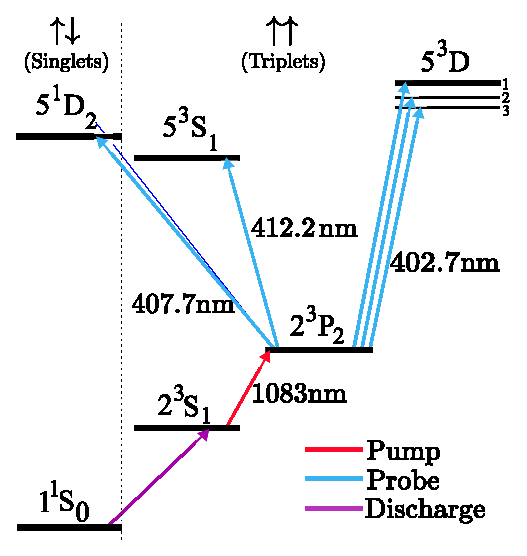
\includegraphics[width=\textwidth]{fig/Spectroscopy/level_diagram_tight_latex.eps}
% 	    \caption{A level diagram for the helium atom. The transitions measured in this work (blue), are driven by a tunable laser referred to in text as the 'probe'. The cooling transition (red) is referred to as 'pump' throughout the paper and populates the lower state of the target transitions.  The doubly forbidden $1\singlet S_0\rightarrow2\triplet  S_1$ transition is excited in a high voltage discharge cell. Transitions between the singlet and triplet manifolds (left and right of dotted line) are forbidden in the dipole approximation. The level splittings are not to scale.}
% 	    \label{fig:lvl_diag}
% 	\end{figure}

% \subsection{Detection scheme}\label{ssec:spec-detection}
% \begin{itemize}
% 	\item Setup - alignment
% 	\item Procedure
% 	\item Mechanism
% 	\item Calibrations
% 	\item Analysis
% \end{itemize}

% \subsubsection{Procedure}
% 	We use a micrometer translation mount on the final lens to align the beam on the Helium sample. We locate the transitions approximately by using the maximum available laser power at the predicted frequency, and then reducing the power and adjusting the frequency set point until the signal no longer saturates at the peak. We then scan the set point of the laser across the transition to obtain the transition signal.
% 	The beam was initially aligned by tuning the probe beam to the predicted value of the 53S1 transition and operating with the maximum available power. Although the uncertainy in wavemeter accuracy was larger than the transition linewidth, by operating well above the saturation intensity, the transition was broaded by tens of MHz and so the WM error was less significant. When scanning the beam pointing across the expected target region, approximate alignment was signaled by a dramatic loss of atom number. When the signal saturated, the power was lowered until the signal was just above the noise floor, and then scanning resumed. This process iterated a few times until the maximum attainable signal was below saturation - that is, when for fixed power one could not completely destroy the trap. Notice there are three kinds of saturation here: Atomic population saturation, detector saturation, and signal saturation when you run out of atoms. perhaps the term `dynamic range' would be more suited to the latter\ldots{} Something to think about.

% 	During the calibration shots, we also block the beam with a mirror mounted on an automatic translation mount. The profile and polarization of the beam are determined with lenses and waveplates prior to vacuum entry. The measurement sequence consists of measurement shots with each of the two magnetic field strengths followed by calibration shots, wherein the laser beam is blocked and switched off. We calibrate the wavemeter before each transition measurement. Analysis of the wavemeter stability suggests that calibration drift is not a significant source of error, as discussed in the supplementary materials.

% 	The method therefore consists of alternating measurement trials with control trials, wherein the laser beam is blocked before the fibre coupler with a flipper mirror. At the moment I use an interpolation, but I might want to try using a model-based estimate of the atom number. Either way, there is going to be some error in the number estimation. It's probably small. The difference between the interpolated, unperturbed atom number and the detected number in the measurement trials is affected by the quantum efficiency and the introduced uncertainty in atom number.

% 	The polarization of the light was fixed with the waveplates before the chamber. Can you tell handedness just by relative angle of waveplates? We hypothesized that the initial state of the atoms during the cooling phase was in the m=2 state, as the optics are configured to drive with a sigma+ beam during the in-trap cooling stage. I verified this by driving with plane-polarized light (in the atom frame - put some trap sim in to show where the field points), which is a linear combination of sigma+ and sigma- light. If there were atoms in initial states other than the m=2, then when driving to the 53S1 state, one would observe multiple peaks. Instead, only one peak was observed, which vanished when the probe beam was set to sigma+ light. (I think check the data).

% 	The measurements are taken at two different background field strengths. Therefore the detuning from cooling resonance is X and Y MHz in each stage, respectively. These values were calibrated independently by an RF spectroscopy technique. This allows empirical extrapolation to the field-free transition energy by correcting for the calculated Zeeman shift of the centre frequency of each measured line.


% % Peak intensity is ~ total power x 1e3 /m^2 for large beam
% \begin{table}
% \begin{tabular}{|c|c|c|c|c|}
% \hline
% Line & Beam waist (cm) & Beam power (mW) &  Peak intensity (W/m$^2$) & Exposure time (ms)\\
% \hline
% $5\triplet S_1$  & 4.1 &  2.73(1) & 3.1(2) & 100 \\
% $5\triplet D_1$  & 4.1 &  4.5(1) & 5.2(1) & 150\\
% $5\triplet D_2,3$& 4.1 &  8.6(1) & 9.9(1) & 250  \\
% $5\singlet D_2$  & 0.1 &  10(2) & 6.3E3 & 100 \\
% \end{tabular}
% \label{tab:spec-beamparams}
% \caption{Probe beam parameters}
% \end{table}
% \begin{table}
% \begin{tabular}{|c|c|c|c|c|}
% \hline
% Stage & Beam power & AOM detuning & Peak intensity & Transition detuning\\
% \hline
% \end{tabular}
% \label{tab:spec-pumpparams}
% \caption{Pump beam parameters}
% \end{table}

% \subsubsection{Data acquisition}
% 	\com{This probably goes in the Intro/BEC machine part}

% 	Following the laser interrogation, the remaining atoms are gradually outcoupled from the trap with a pulsed atom laser. At the beginning of each shot, the LabView control interface writes a line to the log file with the parameters \verb|timestamp, laser_setpt, shot_type| where \verb|shot_type| is either \verb|stage_1|, \verb|stage_2|, or \verb|calibration|. When importing the data into the processing scripts, the 

% 	 As the laser set point is fixed for sets of three shots (one per field setting), 


% \subsubsection{Mechanism of action}
% 	
% 	To drive the transitions from the 23P2 state to the states in the n=5 manifold, I use the probe beam to disturb the near-resonant optical molasses cooling stage of the experiment. This follows the MOT loading and precedes evaporative cooling, and operates with XYZ beam parameters for XXX ms, and then with ABC beam parameters for YYY ms. I calculate that during these stages, the excited-state population is ZZZ per cent, which are then susceptible to scattering photons from the probe beam.

% 	I used the evaporative cooling sequence as a transducer between scattering-induced heating of the cloud and the final condensed number. I will present a quantitative sketch of the mechanism below, but one can also take a heuristic understanding from the following argument:

% 	The evaporative cooling we use to achieve Bose-Einstein condensation has stringent tolerances on initial phase space density, which increases with number and at lower temperatures. Tuning a radio chirp to the spin-flip transition from a trapped to an untrapped state and sweeping down to lower energies, higher-energy atoms are removed, the cloud rethermalizes at a lower temperature, and the phase space density increases. Higher-energy atoms spend time further from the centre of a harmonic magnetic trap. So, scattering photons from the probe beam heat the cloud, leading widening the velocity distribution, which drives more of the atoms into resonance with the radio chirp. The final temperature is determined by the endpoint of the radio chirp. Resonance with the probe light manifests as a signal in a reduction of the final population of the condensate.

% 	As I said, an essential part of our BEC production is an optical cooling and spin-polarizing stage which precedes the loading of our magnetic trap. This ensures a nice large atom number and low temperature. This give us a nice big phase space density, a dimensionless number which compares the length scale of quantum interference, the de Broglie wavelength, with the interparticle spacing given by the particle density n.~So, disturbances to this initial condition by atom loss or heating will reduce the phase space density input to the evaporation stage. The Bose-Einstein condensation threshold occurs when the phase space density crosses about 2 - for comparison, atmosphere has a phase space density about one ten millionth of that. One can therefore think of the RF evaporation as a phase space amplifier in the following way:

% 	Evaporative cooling works by creating a resonance between trapped and untrapped magnetic states of atoms with a specific Zeeman splitting by exposing the cloud to radio frequency radiation. Energetic atoms travel up the magnetic field gradient, shown by the thickness of the purple lines, to the ellipsoidal shell defined by a fixed field strength at which the atoms resonate with the radio waves. The atoms are then transferred into free states and leave the trap, taking with an amount of energy greater than the ensemble average. This basically cuts out the upper tail of the Maxwell-Boltzmann distribution, driving down the atom number, but also the temperature once the cloud rethermalizes. If you get this right, you continuously increase the phase space density by making the cloud cooler and smaller, until you get to BEC. The endpoint of the RF chirp fixes an upper bound to the energy of the trapped atoms, and hence a temperature. Then the phase space density can be estimated by counting the number of atoms you have left. We measure this atom number using Helium's unique detectability - by applying broadband radio pulses to the trap we free about 0.5\% of the atoms at a time, creating a series of pulses of coherent matter waves, known as an atom laser. This resolves on our detector as a series of discrete particle detection events, which we sum up with an abacus. So by controlling our independent variable, the applied laser frequency, we have a gain mechanism that allows us to measure the dependent variable, which is the phase space density reduction by resonant scattering of photons from the probe beam.

% \subsubsection{Calibration measurements}

% 	After the probe is applied during the optical molasses cooling, we use a standard forced evaporative cooling procedure. At the end of the sequence the atoms are in the metastable $2^3S_1$ state which exhibits a 19.8eV ground state separation. This internal energy enables single-atom detection by a multi-channel plate and delay-line detector stack with an efficiency of 8 per cent\cite{Manning10} to determine the atom number loss. We use a pulsed atom laser \cite{Manning10,Henson18} to transfer atoms to the untrapped state and avoid detector saturation.


% 	A translation mount on the final lens gives us micrometer precision in the placement of the focal point on the beam, which we use to align the beam on the trap, threading a ten micron needle in the dark 20 micro-radian accuracy.


% 	\begin{table}
% 	\label{tab:aom_calibration}
% 	\begin{tabular}{|c|c|c|c|}
% 		\hline
% 		RF centre frequency & Calibrated field strength (G) & AOM frequency (MHz) & Detuning (MHz) \\
% 		\hline
% 		XXX & 18 & 138 & 0.5\\
% 		XXX & 11 & 133.6 & 2\\
% 		\hline
% 	\end{tabular}
% 	\end{table}
% 	AO offsets 138MHz and 133.6MHz ?
% 	cooling transition is split 25.55 MHz, and 16.002 in stage 2
% 	Therefore the beams are (ish) detuned 0.5 and 2MHz respectively

% \subsubsection{Analysis}
% 	In this section I describe the data processing method used for the peaks, using the $5\singlet D_2$ line as an example.

% \subsection{Findings}\label{ssec:spec-findings}

% \subsubsection{Results}

% 	\begin{figure*}
% 	  % \includegraphics[width=\textwidth]{fig/Spectroscopy/pub_lines_j1.eps}
% 	  \caption{Measured line profiles for the $\PStateManifold_2\rightarrow 5\triplet  S_1$ (left) and   $\PStateManifold_2\rightarrow 5\triplet  D_1$ (right) transitions, with Lorentzian fits. On the horizontal axis is the probe laser frequency $\nu$, relative to the theoretical prediction for the magnetic field-free splitting. The vertical axis is the response as measured by atom number loss relative to the calibration shots. Theoretical predictions (vertical bars) are Zeeman shifted from the zero-field value according to the field calibration, with uncertainty (horizontal bars) dominated by uncertainty in background field strength. Lines obtained by measuring against an 18G and 11G background field are shown in red and blue, respectively. }
% 	  \label{fig:simple_lines}
% 	\end{figure*}


% \subsection{Determination of transition energies}\label{ssec:spec-processing}


% \begin{figure}
% 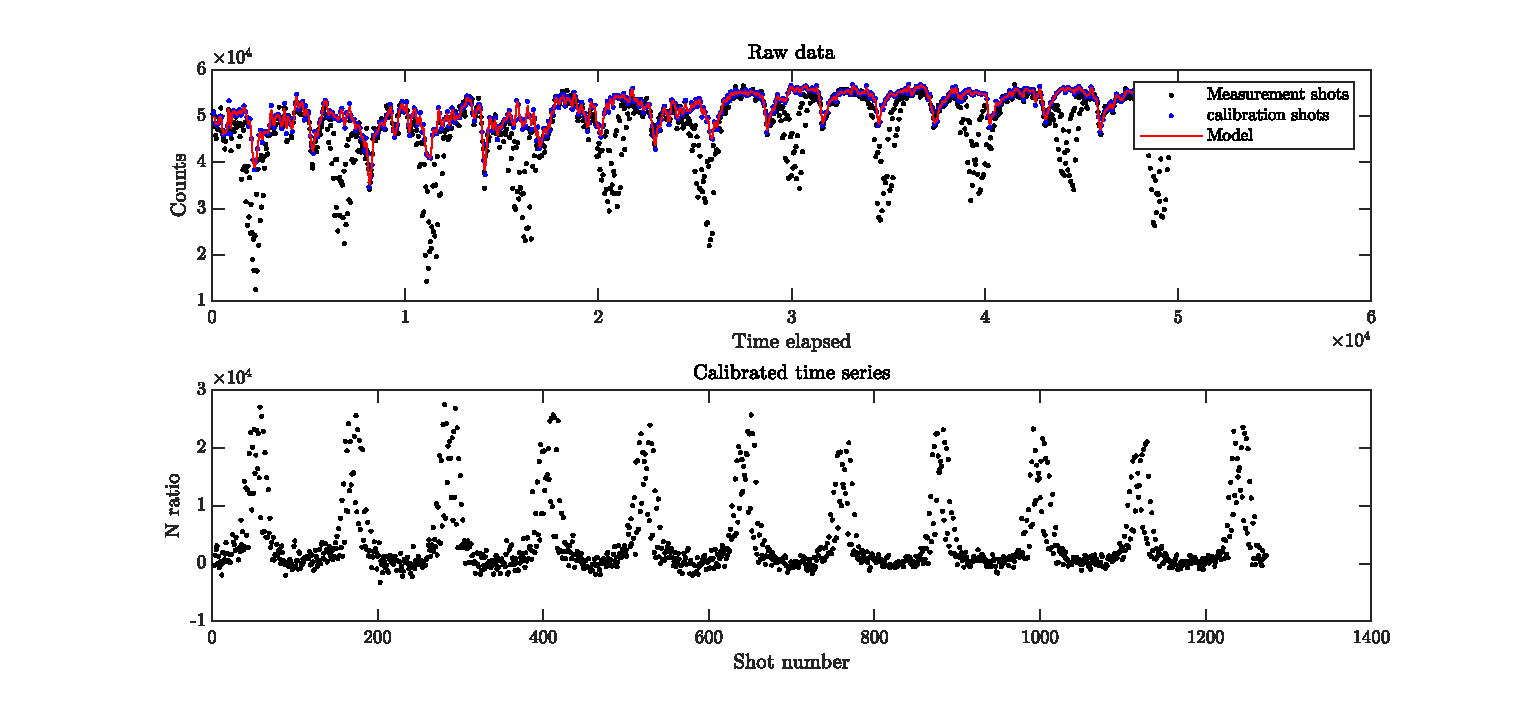
\includegraphics[width=\textwidth]{fig/spectroscopy/calib_model_51D2.eps}
% \label{}
% \caption{}
% \end{figure}

% \begin{figure}
% 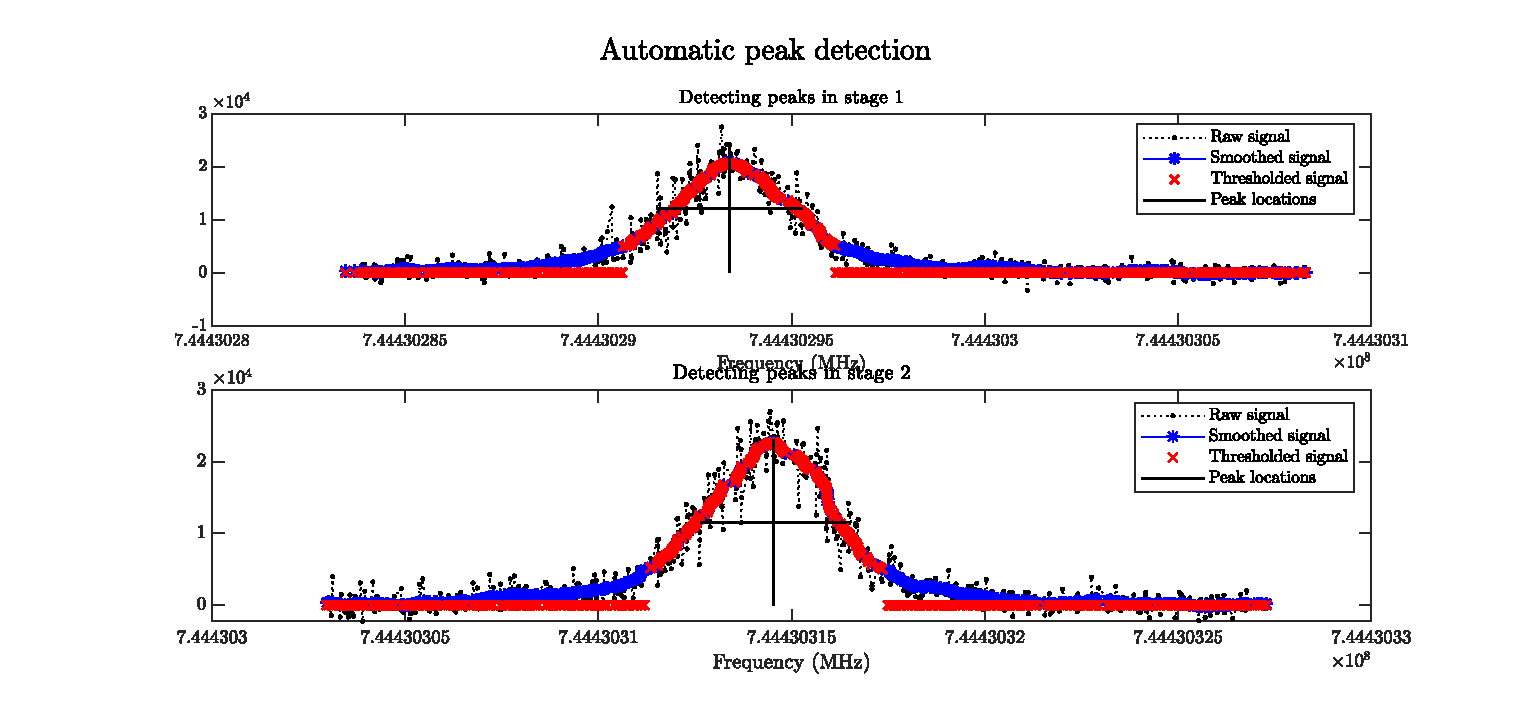
\includegraphics[width=\textwidth]{fig/spectroscopy/auto_peak_detect_51D2.eps}
% \label{}
% \caption{}
% \end{figure}

% \begin{figure}
% 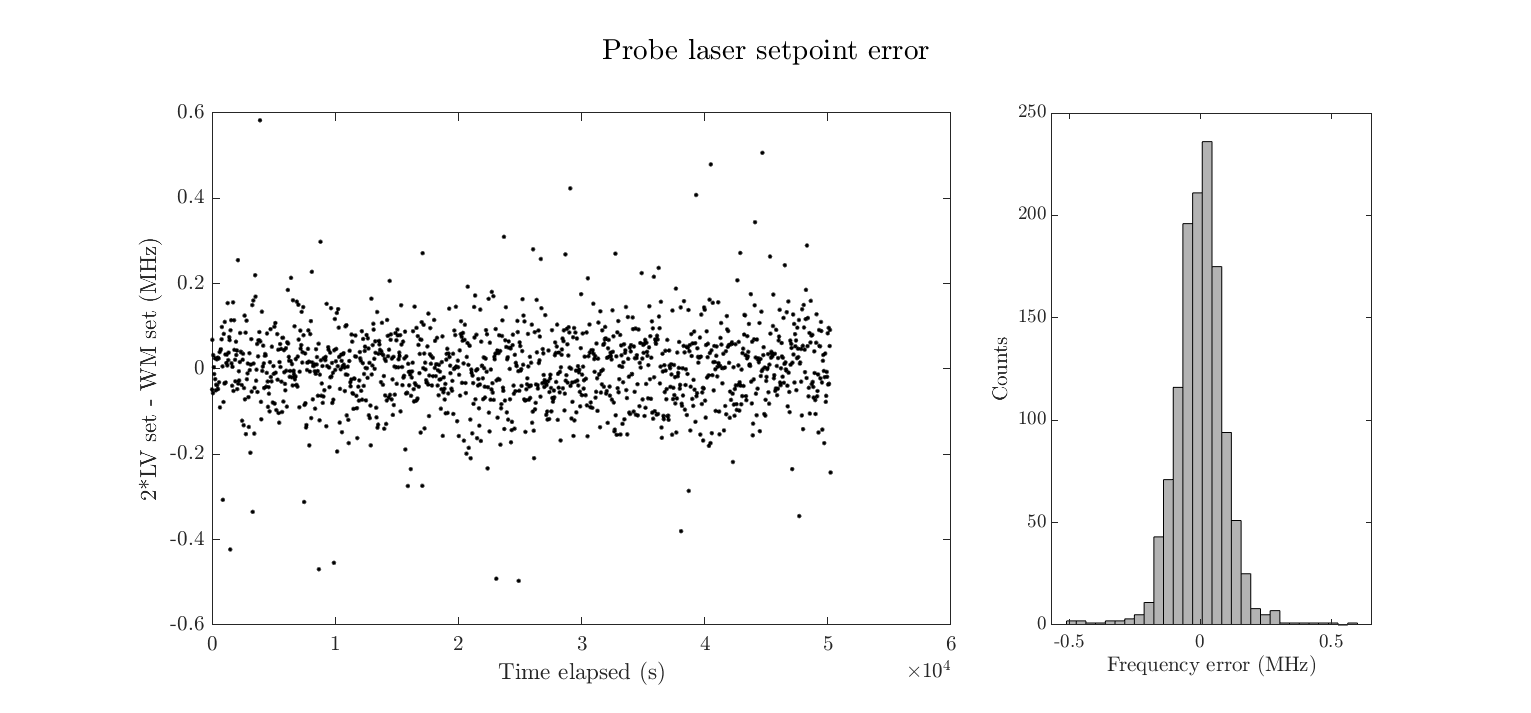
\includegraphics[width=\textwidth]{fig/spectroscopy/probe_set_err_51D2.eps}
% \label{}
% \caption{}
% \end{figure}

% \begin{figure}
% 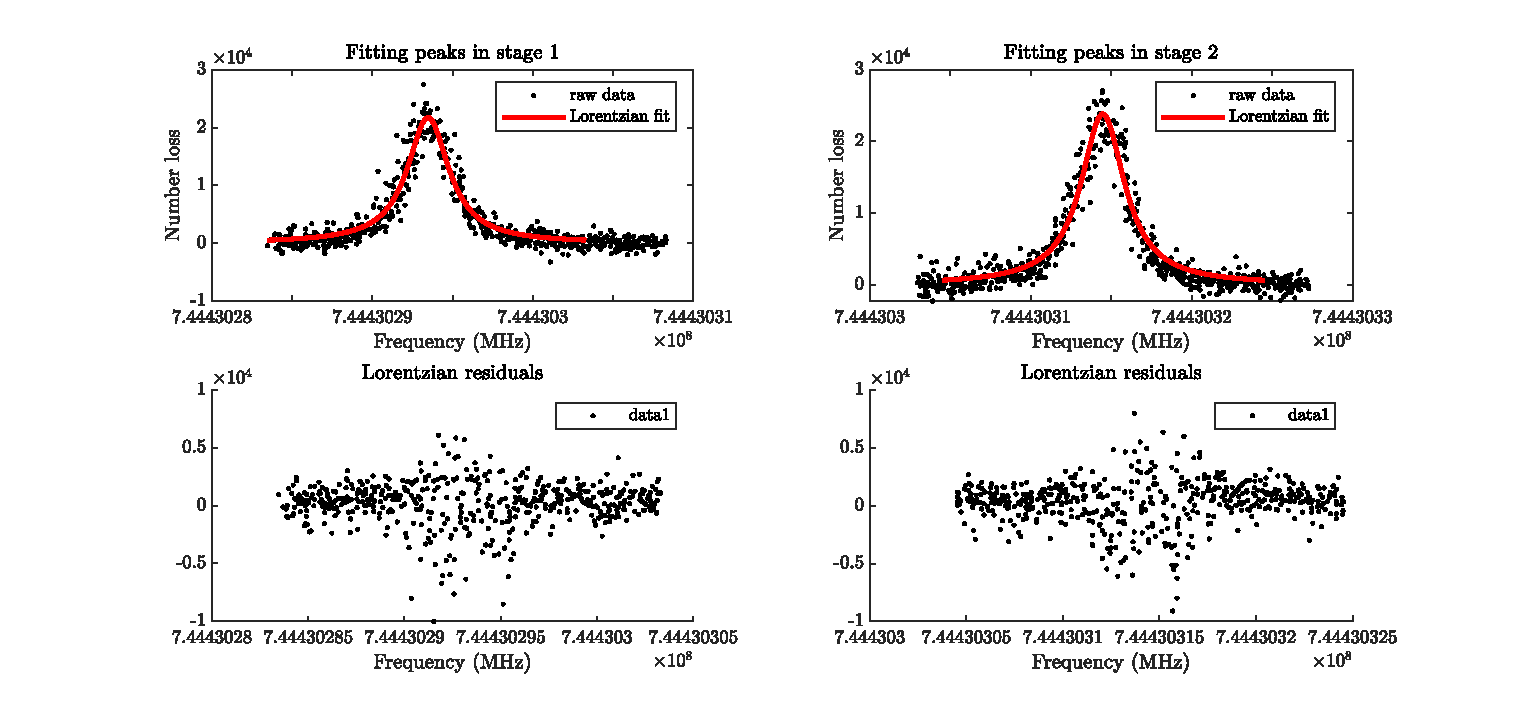
\includegraphics[width=\textwidth]{fig/spectroscopy/fitting_peaks_51D2.eps}
% \label{}
% \caption{}
% \end{figure}

% 	We empirically extrapolate to the field-free transition energy by correcting for the Zeeman shift in the observed lines. The exposure time and intensity varied among measurements to avoid saturation. 

% 	The table below displays the results of the measurements, including predicted linewidths. In the case of the 23S1-33S1, the measured Einstein A coefficient is also listed. These measurements are accurate to a few hundred parts per billion, and their accuracy is limited by the absolute accuracy of the wavemeter we used as a reference for the laser lock. Within the accuracy stated by the manufacturer, these results are consistent with the predictions of QED. Of the six lines measured, three have been resolved individually for the first time, and two have not been recorded elsewhere. The centre frequencies are obtained by fitting Lorentzian profiles to the atom loss spectra. Have a look at residuals; what are the expected broadening effects? What are the expected systematic errors? Error budget goes here also. 	

% 	Ah. The CG madness is only needed for the triplet D states. The singlet D and the triplet S have zero total angular momentum for the spin and orbital dof, respectively, so the basis is trivial and in these cases, we can use the linear extrapolation method with no worries. What about the 2 3P2? Oh - I missed a point, which is the presence of other nearby levels. For the singlet D, that's done, it's unique, as S=0. And for the triplet S, also, as L=0.  Not so for the 2 3P2. But they're several GHz away so that shouldn't be a problem at all. Well, then that's cleared up! Great. Now to write this nonsense up. Start concise in the paper, then we can expand it here. later.

% % A and Sum A from \cite{Drake07}
% % Triplet D: 8.3444E+02 1.3929E+07
% % 5 3S1 line 2.4738E+06 sum 9.2072E+06
% % 5 3DJ sum 1.6412E+07
% % 	Lines
% % 	J=1 3.2224E+05
% % 	J=2 2.8999E+06
% % 	J=3 1.1601E+07
% % 5 1D FROM 2 3P1 402.7151538 nm
% % the 2 3P J=1-2 interval is 2291.177 MHz from Zheng
% % line 8.3444E+02 sum 1.3929E+07
			
% % Two-peak results STAGE 1:

% % Widths: [4.30,5.73,3.03,3.14]
% % Two-peak results STAGE 2:
% % Centres: [744396208.29,744396204.67,744396182.37,744396224.64]
% % Widths: [4.94,4.26,3.91,3.60]

% % Centres_1: [744396195.49,744396191.21,744396160.46,744396223.01]
% % Centres_2: [744396208.29,744396204.67,744396182.37,744396224.64]

% % 3S_1 727303244.61
% % 3D_3 744396209.66
% % 3D_2 744396228.89
% % 3D_1 744396512.43
% % 1D_2 744430344.53

% \begin{table*}
% 	\begin{tabular}{|c||c c|c|c|c|c|}
%     \hline
%         $|e\rangle$ & $f_\textrm{meas,1}$ & $f_\textrm{meas,2}$ & $f_{\textrm{field-free}}$   & $\Delta_\mathrm{theory}$ & $\textrm{FWHM}_\textrm{obs.}$ & $\textrm{FWHM}_\textrm{pred.}$  \\
%     \hline\hline
%         $5^3\mathrm{S}_1$    & 727,303,223.89 &				& 727,303,249(5)   &   4.4    &  3.12(40)& 9.21\\ % A = 
%                              & 727,303,234.04 &				&		& 			 & 		&	\\
%         \hline
%         $5^3\mathrm{D}_1$    & 744,396,453.41 &				& 744,396,496(21) & -16  &  5.79(62) & 16.4\\
%                              & 744,396,477.82 &				& 		& 			 & 	&	\\
%         \hline
%         $5^3\mathrm{D}_2$    &  744,396,191.21 & 744,396,223.01  & 744,396,217(22)  &  -12 & 4.18(50)  &16.4\\
%                              &  744,396,204.67 & 744,396,224.64 & 		& 			 &  &	\\
%         \hline
%         $5^3\mathrm{D}_3$    & 744,396,160.46 & 744,396,195.49 & 744,396,201(21) &  -8.7 & 4.04(12)   &16.4\\
%             			     & 744,396,182.37 & 744,396,208.29  & 		& 			 & 		&\\
%         \hline
%         $5^1\mathrm{D}_2$    & 744,430,295.37 &				& 744,430,347(21) &  2.5  & 3.21(13)  & 13.9\\
%                              & 744,430,316.37 &				& 		& 			 & 		& \\
%         \hline
% \end{tabular}
% \label{tab:spec-results}
% \caption{Summary of results (all in MHz) For each transition. The measured frequencies are obtained in an ambient magnetic field of strength 18G (top row) and 11G (bottom row). After correcting for the AOM and vapor cell shifts we extract the centre frequencies $f_{meas}$ from Lorentzian fits with statistical error at the $~ 10\textrm{kHz}$ level. For the $5\triplet D_2$ and $5\triplet D_3$ states, each line shows the pair of transitions corresponding to the magnetic quantum number of the upper state $m_u=1$ and $m_u=2$, respectively. After correcting for Zeeman shifts, the field-free energies $f_{\textrm{field-free}}$ are obtained, and shown with statistical error in parentheses. We show the difference $\Delta_\mathrm{theory}$ between our measurements theoretical predictions \cite{Drake07}. Observed line widths are the mean full width at half maximum $\textrm{FWHM}_\textrm{obs.}$ of a Lorentzian fit to each line, with theoretical predictions $\textrm{FWHM}_\textrm{pred.}$ from \cite{Drake07}.}
% \end{table*}
% 	\begin{figure}
% 	  % \includegraphics[width=\textwidth]{fig/Spectroscopy/pub_lines_5D1.eps}
% 	  \caption{Line profile for the spin-forbidden $\PStateManifold_2\rightarrow 5\singlet D_2$ transition, presented similarly to figure \ref{fig:simple_lines}.}
% 	  \label{fig:3D_1_line}
% 	\end{figure}


% 	\begin{figure}
% 	  % \includegraphics[width=\textwidth]{fig/Spectroscopy/pub_lines_5D2_3.eps}
% 	  \caption{Line profiles for the $\PStateManifold_2\rightarrow 5\triplet  D_{2}$ and $\PStateManifold_2\rightarrow 5\triplet  D_{3}$ transitions, driven by a mixure of $\sigma^-$ and $\pi$- polarized light and presented similarly to figure \ref{fig:simple_lines} and \ref{fig:3D_1_line}. The large central peak is the overlap of two peaks, the transitions to the XXX and YYY lines, which are nearly degenerate for the entire operational range of our background magnetic field.}
% 	  \label{fig:3D_23_lines}
% 	\end{figure}
% 	Figure 2 shows the spectra measured using this technique. Table I summarizes the results of our measurements. An account of our error budget is given in the supplementary materials, and summarized in Table II.  While we are able to resolve the $5\triplet  D_1$ peak, the $5\triplet  D_2$ and $5\triplet  D_3$ resonance are sufficiently close together to cause significant quantum interference effects \cite{Marsman15}, and require special treatment to obtain the zero-field values. 

% \subsubsection{Error budget}

% 	The statistical error in the centre frequency of our Lorentzian fits is less than a MHz, fixing these transitions to some parts per billion, with MHz differences from theory. The last measurement of the 2\textsuperscript{3P-5}3D gap could not resolve the fine structure splitting, about 300MHz, but we resolve them with excellent visibility. To give credit where credit is due, the last measurement of these transitions used a discharge cell submerged in liquid nitrogen, passed through a window to an in-vacuum diffraction grating and illuminating a phosphor screen with lines whose splitting was measured with a ruler against a Mercury reference. Still, they were wrong.

% 	But, our ultimate accuracy is limited by the wavemeter to 20MHz in the worst case, or 4MHz when close enough to the calibration line. Unfortunately, we don't have the precision required to compete with the state of the art, but had we a frequency comb reference then we'd be in the game for tests of fundamental physics. Still, we correct the previous values by thirteen gigahertz, update four values in the NIST database, and add a new line to boot. We conclude that within our experimental uncertainty, QED is correct.

% 	The AC Stark effect from the probe beam varies between the measurements, but in all cases is calculated to be less than 1MHz, in agreement with an empirical determination described in the supplementary materials. The recoil shift is ambiguous in sign because of the counterpropagating pump beams, but the shift is at least an order of magnitude less than the absorption linewidth.

% 	\begin{table}[h]
% 	\begin{tabular}{|c|c|c|}
% 	    \hline
% 	        Source & Shift (MHz) & Unc. (MHz)  \\
% 	    \hline\hline
% 	        AC Stark (Pump) & $<$0.1 & -\\
% 	        AC Stark (Probe) & $<$1 & -\\
% 	        DC Stark & $<$0.1 & - \\
% 	        Mean field & $<$0.1 & -\\
% 	        Recoil & $\pm0.218$ & 1 \\ % assume angle accurate to 1deg
% 	        Wavemeter & 0 & Variable \\
% 	        Doppler & XX & YY \\
% 	        Pump lock & N/A & 0.3 \\
% 	        Probe lock & -190MHz & 0.1\\
% 	        Cs cell & -1.9 & 4 \\
% 	    \hline
% 	        Total & -1.9&4.1+WM\\
% 	    \hline
% 	\end{tabular}
% 	\caption{Error budget for the measured lines. }
% 	\end{table}

% \subsubsection{Discussion}

% 	We improve on previous measurements with an order of magnitude greater precision and report the first observation of the spin-forbidden $2\triplet  P_2\rightarrow5\singlet D_2$ transition in Helium. Our measurements constrain the $5\triplet  D$ and $5\singlet D$ ionization energies of $^4$He to 150 parts per billion, and the $5\triplet  S$ $5^3S$ to 28 parts per billion. The theoretical transition energies agree with the observed values within experimental error.

% 	We performed multilevel laser absorption spectroscopy of excited states with ultracold atoms in hard vacuum. Our measurements agree with current predictions within our error budget. A $93\sigma$ difference between Martin's measurement\cite{Martin60} and predictions \cite{Morton06} of the $\PStateManifold_2 \rightarrow \UpperS$ and $\PStateManifold_2 \rightarrow \UpperStateManifold$ intervals are resolved by this work.  Our measurements constrain the $5^3D$ and $5^1D$ ionization energies of 4He to 150 parts per billion, and the $5^3S$ to 28 parts per billion. This work provides four contributions to the NIST database of atomic spectral lines. 

% 	In Martin's original paper, he only quotes measurements from $\PStateManifold_2-5D$, indicating that his equipment did not have the resolving power to distinguish the fine structure of the $5D$ state. Martin's measurements were made using a nitrogen-cooled Helium discharge lamp fed through an in-vacuum prism onto photographic plates where line separations were measured with a ruler. 

% 	The apparatus used for this experiment is presently being upgraded to operate with $^3$He - $^4$He mixtures. This technique could be employed, along with an improved frequency reference such as a clock-stabilized frequency comb, to constrain the charge radius difference for comparison with other transitions.



% \section{Detection of the forbidden $2\triplet  S_1\rightarrow3\triplet  S_1$ transition}\label{sec:forbidden}

% 	After our measurement of the 2P-5L transitions, our eyes turned to the 427nm transition. To our knowledge, nobody had measured it. We found that we required ten orders of magnitude greater sensitivity in order to detect this transition - a few mW over a few ms wasn't going to cut it. After discussion we decided that the most promising method might be to look for heating or loss by directly illuminating a BEC - having found previously that weak trap lifetimes can in fact be several minutes. However, before we embarked on the measurement, I performed some simple calculations to estimate the order of magnitude of the best signal-to-noise ratio we could expect.

% 	We determined that this SNR would be sufficient to warrant making an attempt at the measurement.

% 	RECOUNT CALCULATION * 3 level measurement * Clebsch-gordan coefficients
% 	and net transition rates * Collection efficiency monte carlo

% 	For this measurement, the data processing methods were the similar to the 5L transitions - a drift model was created to predict the undisturbed atom number in a given shot, based on atom number measurements from the calibration shots. Wait - did the outcoupled fraction get used, counting the number dropped versus the number left in the trap? Were these things tried? Talk to Kieran.

% 	This method allows for the extraction of the line centre and width, which determines the state lifetime. However, the state lifetime is dominated by a fast decay to the 3P state, the oscillator strength of which is many orders of magnitude larger. The oscillator strength - which is proportional to the Einstein A coefficient - of the transition can be obtained by another method, described in the next section.

% 	We develop a second method to determine the Einstein A coefficient of the specific forbidden transition. We perform time-dependent thermometry of the a thermal cloud (above the critical temperature) while alternating shots with and without the probe beam blocked. During these sequences, we use RF pulses as per standard procedure (although in this case the term `laser' is especially misleading as the source is incoherent) and fit a Gaussian profile to each pulse. During the 25 second hold time, the cloud heats at a rate of X K/sec.~This is possibly due to: Penning ionization, magnetic field noise, background collisions, majorana leaks? How does it depend on number? Anyway. With the probe beam applied, the calculated scattering rate of up to Y Hz corresponds to a peak additional heating rate of Y J/sec.

% 	We fit the time evolution of the temperature of the thermal cloud with a linear model and obtain the change in heating rate with respect to the probe-free shots. We can then back-calculate via the specific heat of a harmonically trapped Bose gas to determine the energy transfer rate (which should just be proportional I think, when above the critical temperature?), hence the photon scattering rate. And so lo and behold we can determine the A coefficient, and look, it's really weak! What a great job we did. I wonder whether Kieran's method is a bit sketch because does heassume a certain density distribution??

% 	Power \& curvature measurements - what actually drives Quadrupole
% 	transitions?
% \subsection{Proof-of-feasibility calculation}\label{ssec:forbidden-feasibility}
% \subsection{Two detection methods}\label{ssec:forbidden-methods}
% \subsection{Findings}\label{ssec:forbidden-findings}
% \subsubsection{Error budget}
% \subsubsection{Results}

% 	Isotope shifts \& better reference 
% 	Different target transitions?

% https://physics.stackexchange.com/questions/430532/why-are-there-no-transitions-between-orthohelium-and-parahelium





% 
% https://en.wikipedia.org/wiki/Proton_radius_puzzle
%  Contains some refs showing that theory-motivated fits can be a good idea
% \newcommand{\org}[1]{{\begin{color}[rgb]{1.0,0.5,0}{#1}\end{color}}}



\chapter{Precision measurement of the 413 nm tune-out point}
\markboth{\thechapter. MEASUREMENT OF THE 413 nm TUNE-OUT}{}
\label{chap:tuneout}

\blankfootnote{\noindent The contents of this chapter relate to the work published in \textbf{Measurement of a helium tune-out frequency: an independent test of quantum electrodynamics} by B. M. Henson$^\dagger$, {J. A. Ross}$^\dagger$, K. F. Thomas, C. N. Kuhn, D. K. Shin, S. S. Hodgman, Y. H. Zhang, L. Y. Tang, G. W. F. Drake, A. T. Bondy, A. G. Truscott, K. G. H. Baldwin, \href{https://www.science.org/doi/10.1126/science.abk2502}{\emph{Science} \textbf{376}} (2022) ({$^\dagger$\emph{Equally-contributing authors})}}


	\begin{flushright}
	\singlespacing
	{\emph{``Turn on\\
			Tune in\\
			Drop out"\\} 
	Tim Leary \cite{LearyNote}.}
	\end{flushright}
	\onehalfspacing
	\vspace{1cm}
	% \end{adjustwidth}

	



	\noindent{Nothing} in the universe is truly motionless, as imposed by the ineradicable zero-point energy and uncertainty principle.
	And yet, atoms may be unmoved by an electric field if the latter oscillates at a \emph{tune-out} point.
	In vacuum conditions, the specification of the wavelength, frequency, or photon energy of light are all equivalent. 
	Thus, I use the encompassing term `tune-out point' where the context does not favour any particular unit of measurement.
	However, in keeping with the tendency in metrology, the quantity of interest in this chapter is the tune-out \emph{frequency}, or simply \emph{tune-out} for brevity. 
	In the publication pertaining to this chapter (Ref. \cite{Henson22}) we introduced the notation $L-U_1/U_2$ to specify a tune-out point by the occupied state $L$ followed by the two transitions $U_1$,$U_2$ which dominate the polarizability at the specified tune-out. 
	This chapter concerns the measurement of the frequency of the $\MetastableState-2\triplet P/3\triplet P$ tune-out point near 413 nm (726 THz) \cite{Henson15,Mitroy13} and a comparison with state-of-the-art atomic structure calculations as a test of quantum electrodynamics.
	Interestingly, the tune-out point is usually determined by the position and strength of the nearest transition frequencies. 
	However, in this case the tune-out is principally controlled by the $2\triplet P$ and $3\triplet P$ levels (with transitions at 277 and 771 THz, respectively) despite the $3 \triplet S_1$ being only $701$ THz away. This is because the  $\MetastableState \rightarrow 3^{3\!}S_1 $ transition is extremely weak\footnote{We detected this transition during the laser spectroscopic campaign which included the present and prior chapters. As reported in Ref. \cite{Thomas20}, this is at present the weakest transition detected in a neutral atom.}.

	As this work constitutes the most detailed work undertaken in the course of study, and the longest chapter, a brief mention is warranted of the way ahead.
	Section \ref{sec:TO_bg} includes a detailed definition of a tune-out point with aid of semiclassical models along the way. This section also discusses the motivation for the work and a short summary of the theoretical progress made in parallel to the experimental measurement, which is reported in section \ref{sec:trap_freq_measure}. The foci of section \ref{sec:trap_freq_measure} are the description of the physical process underpinning the probe and measurement methods, including a fine-grained discussion of the effects of the frequency and polarization of the probe laser at the interaction zone. Having established the working principles of the measurement, section \ref{sec:TO_analysis} gives an end-to-end account of the data analysis. This section covers the criteria for diagnosing failure modes and discarding aberrant data files, the extraction of a final measured value and quantifying its statistical confidence, and some sanity checks to assure ourselves that our model maps well onto the ground truth. Section \ref{sec:systematic_effects} enumerates the systematic effects that we quantified in order to determine the ultimate accuracy of the measurement. Finally, section \ref{sec:TO_discussion} summarizes the findings of the experiment, including the establishment of a handful of figures-of-merit and a claim to a new sensitivity record.

	
\section{Background}
\label{sec:TO_bg}

\subsection*{Feynman's jewel}
	% \com{Keeping the phrasing from the paper; at the final stages it was written largely by myself with Kieran's help}
	Quantum electrodynamics describes the interaction between matter and light, an interplay so ubiquitous that the theory is regarded a cornerstone of modern physics.
	QED has yielded extraordinarily accurate predictions about fundamental processes such as spontaneous emission rates of photons from atoms and the anomalous electron magnetic moment \cite{Aoyama15}.
	However, despite withstanding decades of stringent testing against high-precision measurements, recent results in atomic spectroscopy have revealed discrepancies between experiment and theory.  
	With the precision of atomic spectroscopy approaching the part-per-trillion level, the `proton radius puzzle' has emerged, wherein determinations of the proton radius from spectroscopic measurements (of muonic \cite{Pohl10} and eletronic hydrogen \cite{Bezginov19,Beyer17}, and of muonic deuterium \cite{Pohl16}) disagree by up to five standard deviations with other approaches (electron-proton scattering \cite{Zhan11} and hydrogen spectroscopy\cite{Fleurbaey18}). 


	Helium is an exemplary system for complementary tests of QED thanks to its simple two-electron structure, which makes high-precision predictions tractable and testable. 
	Notably, helium presents a nuclear `puzzle' of its own: precision measurements of the isotope shifts of the \(\MetastableState \rightarrow \LowerStates \) \cite{Zheng17} and \(\MetastableState \rightarrow \SingletState \) \cite{Rengelink18} transitions disagree by two standard deviations in the derived nuclear radius shift $r(^4\textrm{He})^2-r(^3\textrm{He})^2$. 
	Further, recent measurements of the ionisation energy for the helium $2^{1\!}S_0$ state \cite{Clausen21} confirm similar discrepancies in the Lamb shift to those recently revealed theoretically \cite{Patkos21}.
	These puzzles raise the possibility that QED itself may be a flawed jewel \cite{Hill17} - and that some new physics may be within experimental reach in the atomic physics laboratory. 

	The tune-out frequency, where an atom feels no force resulting from applied laser light, is an observable that tests QED independently of the conventional measurement of energy level differences.
	We selected the $\MetastableState-2\triplet P/3\triplet P$ tune-out as our target quantity because the nearest two transitions are separated by more than an octave, and thus the atomic polarizability must vary slowly with optical frequency near the tune-out. 
	Therefore, this tune-out is especially sensitive to higher order QED effects. 
	We achieve a 15-fold improvement in the precision over the sole previous measurement (which was also undertaken in the ANU \mhe lab \cite{Henson15}) and make a definitive comparison with theory thanks to a new theoretical prediction of the \(\TO\) tune-out (summarized in section \ref{sec:to_theory}).
	The experimental value of 725\,736\,700\,$(40_{\mathrm{stat}},260_{\mathrm{syst}})$~MHz is within \({\sim} 2.5\sigma\) of the predicted frequency (725\,736\,053(9)~MHz),   resolving contributions from QED effects (\({\sim} 30 \sigma\)) and probes finite-wavelength retardation corrections (\({\sim} 2 \sigma\)) for the first time, albeit with lower confidence.


\subsection*{Tune-out points}
\label{sec:TO_points}
\begin{figure}
		\centering
		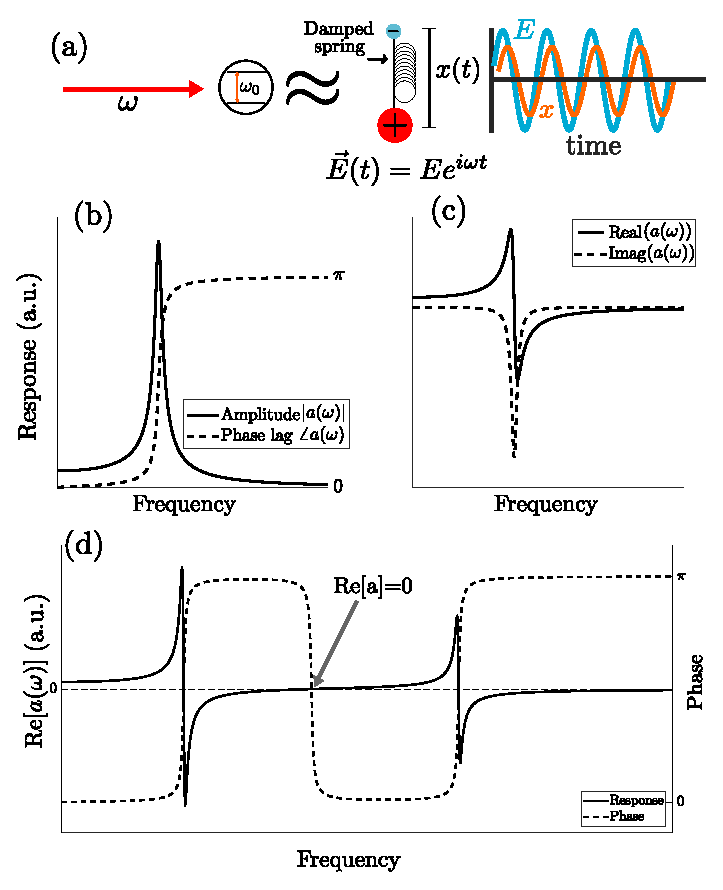
\includegraphics{fig/tuneout/lorentz_model}
		\caption{(a) Illustration of the Lorentz oscillator model of polarizability, wherein the dipole moment of atom in an off-resonant light field is approximated by a periodically driven mass-spring system. The response function (b) has a peak at the resonant frequency $\omega_0$, about which the phase of the response flips from 0 to $\pi$. The spectrum (c) shows that at the zero-crossing of the phase, the steady-state amplitude (real part) of the response is zero but the imaginary part is negative, indicating absorption of energy from the driving force (resonance). A multi-level atom can be approximated by the superposition of such oscillators which give rise to multiple resonances (d). Between the resonances there is also a sign-flip of the phase, coincident with a zero-crossing of the real part. The position of these 'tune-out' points depends on the positions and relative strengths of the resonances.}
		\label{fig:lorentz}
	\end{figure}
	
	Recall from chapter \ref{chap:theory} that an atom in an oscillating electric field experiences an energy shift.
	The magnitude of this shift is proportional to the real part of the dynamic polarizability $\alpha(f)$, a fundamental atomic property determined by the frequency $f$ of the oscillating electric field, the spacing of energy levels, and the strengths of the respective dipole matrix elements.
	This can be illustrated by the classical Lorentz model which approximates the atomic dipole moment by a fixed positive charge plus a negatively-charged particle attached to the `nucleus' by a spring (illustrated in Fig. \ref{fig:lorentz})\footnote{An equivalent model can be constructed using an LC circuit.}.
	The object of ultimate interest is the equation of motion, which in the Lorentz model is 
	\begin{equation}
		\ddot{x} + \Gamma \dot{x} + \omega_0^2x = -e\vec{E}/m.
	\end{equation}
	Here, $m$ is the mass of the `electron' and the spring has resonant frequency $\omega_0$ and damping rate $\Gamma$, as illustrated in Fig. \ref{fig:lorentz}.
	The general solution for the equation of motion has the form $x(t) = a(\omega)|\vec{E}|e^{i\omega t}$, whose frequency spectrum has a Lorentzian profile,
	\begin{equation}
		a(\omega) = -\frac{e}{m}\frac{1}{(\omega_0^2-\omega^2)+i\Gamma\omega},
	\end{equation}
	where the real part gives the steady-state amplitude of the induced oscillation, and the imaginary part relates to the exchange of energy from the electric field.
	In fact, a real atom possesses many resonances and to first order (in the linear-response regime) the total response is the sum over all resonances, as in $a(\omega) = \sum_i A_i a_i(\omega)$. 
	Thus there generally exist points in the spectrum where the real part of $a(\omega)$ vanishes, which are determined by the resonant frequency and oscillator strength of each possible transition from the current state of the atom.
	
	In the quantum picture a similar correspondence holds: The real part of the polarizability $\alpha(\omega)$ gives the energy shift as a result of a perturbing light beam, and the imaginary part fixes the photon scattering rate  via $\Gamma_{sc} = \textrm{Im}(\alpha)I/(\hbar\varepsilon_0 c)$ in a monochromatic light field with intensity $I$. 
	For a multilevel atom in the state $i$ under the dipole- and rotating-wave approximations \cite{Grimm00} the Stark shift is
	
	\begin{align}
		\Delta E &= -\frac{1}{2\epsilon_0 c}\mathrm{Re}(\alpha(f))\\
		 	&= -\sum_{j\neq i}\frac{|\bra{j}\hat{\mu}\cdot\mathrm{\textbf{E}}\ket{i}|^2}{E_i-E_j}
			% &= -\sum_{j\neq i}\frac{F_{ij}?}{E_i-E_j},		 	
		\label{eqn:dipole_shift}
	\end{align}
	
	\noindent where the $E_i$ are the unperturbed energies, and $\hat{\mu}\cdot\mathrm{\textbf{E}}$ is the dipole interaction energy.
	In the quantum-mechanical framework the strength of these resonances is characterized by the oscillator strengths $f_{ij}$, which are proportional to the (squared) matrix elements $|\bra{j}\hat{\mu}\cdot\mathrm{\textbf{E}}\ket{i}|^2$.
	A ‘tune-out’ frequency (labeled $f_\mathrm{TO}$) occurs between transition frequencies at the point where the contributions to the dynamic polarizability\footnote{For brevity, and as we are concerned solely with the real part of the polarizability, we will simply use the notation $\alpha(f)$ to refer to the \emph{real} part of the polarizability.} $\alpha(f)$ from transitions below that frequency are balanced by those above it (i.e. $\alpha(f)=0$) \cite{LeBlanc07}. 
	This balance point, illustrated in Fig. \ref{fig:he_polz} is therefore fixed by the strength (via the numerator in the RHS of Eqn \ref{eqn:dipole_shift}) and frequency (via the denominator) of every transition in the atomic spectrum and thus provides a precise constraint on the ratio of transition dipole matrix elements. 
	The frequency-dependend polarizability for \mhe~is also shown in Fig. \ref{fig:he_polz} spanning just under 2.5 octaves.

	\begin{figure} 
		\centering
		\includegraphics[width=\textwidth]{fig/tuneout/composite_polz_fig}
		\caption{Tune-out in atomic helium:
		(A) Atomic energy level shift of the dominant state (manifolds) about the tune-out.  When an optical field of frequency $f$ (arrows) is applied to the atom the individual
		levels shift dependent on the difference between $f$ and the transition frequency. At the tune-out frequency $f_{\mathrm{TO}}$ (middle right), the shifts to the $\MetastableState$ state energy cancel.
		Energy spacing and shifts not to scale.
		(B) Theoretical frequency dependent polarizability of $\MetastableState$ helium, for a constant light polarisation, indicating that the polarizability vanishes near 726~THz, - the tune-out frequency measured in this paper. 
		Vertical dotted lines show, from left to right, the transitions to the  $\TOLowerStateManifold$, $\TOUpperStateManifold$,$4^{3\!}P$ manifolds. Inset shows the approximately linear polarizability with frequency about the tune-out.
		}
		\label{fig:he_polz} 
	\end{figure}



\subsection{Polarizability near $\fto$}
\label{sec:polz_linearization}

	% % in \cite{LeKien13}
	% % [17,18,20] scalar and tensor polz calculated for Sr and [21,22] For Cs motivated by calculation of magic wavelengths
	% % [16] variety of ways to calculate polarizabilities
	% % [17-19] magic wavelengths are those for which both upper and lower states of a transition are shifted by equal amounts 
	% % [23,24] tune-out wavelength searches for alkali-metal atoms
	% % [25] there are three components, scalar tensor and vector
	% % [33] calc sof SVT polz for Rb
	% % [37] imaginary part of polz is related to the scattering rate

	% The time-dependent polarization of an atom in response to a time-varying electric field is governed by the dynamical polarizability \cite{LeKien13}.
	
	The atomic polarizability has a complex profile, as shown in Fig. \ref{fig:he_polz}, but as we are concerned with measurements in a small region around a tune-out point, we can simplify the analysis below by linearizing the polarizability with respect to frequency. This assumption breaks down if one were to make measurements over much wider frequency intervals, and the magnitude of the loss of accuracy is quantified in section \ref{sec:systematic_effects}.
	In the rest of this section, I describe how the tune-out depends on the frequency and polarization of the laser light, and how this allows us to select a single figure of merit for comparison with theoretical clculations.

	Consider the interaction of an atom with a (real-valued) electric field with the form
	\begin{equation}
		\mathbf{E} = \frac{1}{2}\left(\vec{\mathcal{E}}e^{-2\pi i f t}+\vec{\mathcal{E}}^*e^{2\pi i f t}\right),
	\end{equation}
	where $\vec{\mathcal{E}}=\mathcal{E}\hat{\mathbf{u}}$ is the electric field envelope with magnitude $\mathcal{E}$, polarization vector $\mathbf{u}$ (which may be complex), and oscillation frequency $f$.
	Hereafter in this section, we will consider the atomic reference frame defined by a quantization axis $z$. For a far-off-resonant light field, the Stark shift will be small compared with the fine-structure level splitting. 
	In this case, and working in the dipole appoximation \cite{LeKien13}, the interaction energy between the atomic dipole $\mathbf{d}$ and the light field is captured by the operator
	\begin{equation}
		\Delta E_\mathrm{Stark} = -\frac{1}{2}\left(\mathcal{E}\mathbf{u}\cdot\mathbf{d}e^{-2\pi i f t} - \mathcal{E}^*\mathbf{u}^*\cdot\mathbf{d}e^{2\pi i f t}\right),
	\end{equation}
	which, after a lengthy derivation \cite{LeKien13} can be written as
	\begin{align}
		\Delta E_\mathrm{Stark} &= -\frac{1}{2\epsilon_0 c} \mathrm{Re}(\alpha(f)) I
	\end{align}
	where $I= \frac{\epsilon_0 c}{2} |E|^2$ is the electric field intensity and
	\begin{equation}
		\alpha(f) = \alpha^S + C\alpha^V \frac{m_J}{2J} + D\alpha^T\frac{3m{_J}^{2}-J(J+1)}{2J(2J-1)}
		\label{eqn:full_polz}
	\end{equation}
	% note I = c \epsilon_0 |E|^2/2 so the first line is just Re(a)E^2/4
	is the frequency-dependent polarizability for an atom in a state with total angular momentum $J$ (and a $z$-component of $m_J$).  
	The frequency-dependent scalar, vector, and tensor polarizabilities are $\alpha^S$, $\alpha^V$, and $\alpha^T$, respectively, and the coefficients $C=2\mathrm{Im}(\mb{u}_{x}^{*}\mb{u}_{y})$ and $D= 3|\mb{u}_z|^2-1$ depend on the polarization vector $\mathbf{u}$. More will be said about the polarization effects in section \ref{sec:polz_dep}, but for now let us return to the frequency-dependent effects.
	From the preceding equation \ref{eqn:full_polz} one then obtains the polarizability for the $2\triplet S_1(m_J=1)$ state:
	\begin{equation}
		 \alpha(f) = \alpha^S(f) + \frac{1}{2}\left(C\alpha^V(f)  + D\alpha^T(f)\right).
		 \label{eqn:master_polz}
	\end{equation}
	% in this eqn, D = 3 |u_z|^2 -1, opposite to the Le Kien convention
	Expanding the preceding equation about some frequency $f_0$ near $\fto$ we and truncating the Taylor expansion we have
	\begin{align}
		 \alpha(f)  \approx & \alpha^S(f_0) + (f-f_0)\frac{d\alpha^S}{df}\Bigr|_{f=f_0} \\
		 &+ \frac{C}{2}\left(\alpha^V(f_0) + (f-f_0)\frac{d\alpha^V}{df}\Bigr|_{f=f_0} \right)\\
		 & +\frac{D}{2}\left(\alpha^T(f_0) + (f-f_0)\frac{d\alpha^T}{df}\Bigr|_{f=f_0} \right) + \cdots
	\end{align}
	It is expected on theoretical grounds that the vector and tensor polarizabilities are nearly constant over the scan ranges we use in this experiment (and we can check this experimentally - indeed we do find that the gradient of the fits $\propto d\alpha /d f$ is independent on the polarization, thus only the $\propto d\alpha^S /d f$ is significant).	Hence, we can drop the respective derivative terms and arrive at

	\begin{align}
		 \alpha(f)  \approx & \alpha^S(f_0) + \frac{d\alpha^S}{df}\Bigr|_{f=f_0} (f-f_0) + \frac{C}{2}\alpha^V(f_0) + \frac{D}{2}\alpha^T(f_0).
		 \label{eqn:polz_taylor}
	\end{align}
	The condition that $\alpha(\fto)=0$ implies
	\begin{align}
		 \frac{d\alpha^S}{df}\Bigr|_{f=f_0} (\fto-f_0) \approx & -\alpha^S(f_0) - \frac{C}{2}\alpha^V(f_0) - \frac{D}{2}\alpha^T(f_0).
	\end{align}
	We can simplify this result by setting $f_0$ to be the tune-out for the scalar polarizability, i.e. $f_0=\fto^S$ s.t. $\alpha^S(\fto^S)=0$, thus arriving at
	\begin{align}
		 \fto \approx & \fto^S - \frac{C}{2}\beta^V(\fto^S) - \frac{D}{2}\beta^T(\fto^S)
		 \label{eqn:redpolz}
	\end{align}
	\begin{equation}
		\beta^X(f) = \alpha^X(f)\left(\frac{d\alpha^S}{df}\Bigr|_{f=f_0}\right)^{-1}
	\end{equation}
	for $X\in\{V,T\}$.

	The main conclusions of the preceding calculations is that the polarizability is well-approximated by the linearized equation (\ref{eqn:polz_taylor}) for experimentally relevant detunings from the tune-out. The change in polarizability with respect to frequency is dominated by the scalar term $\alpha^S(f)$, but the zero-crossing of the total polarizability $\alpha(f)$ is modified by the polarization-dependent terms ($\frac{C}{2}\beta^V(\fto^S)$ and $\frac{D}{2}\beta^T(\fto^S)$). Therefore, the tune-out frequency depends on the polarization of the laser beam (Eqn. (\ref{eqn:redpolz})), and so we need to establish some terminology to relate the beam parameters to the atomic dipole response. As we will see below, this also permits us to define a single measurable quantity that can be compared directly with theory.

	% Tang: When A cos \theta_k is adjusted from -1 to 1 the TO shifts by 0.4-6 pm 
	% We must specify a quantity in order to make an unambiguous comparison with theoretical calculations, and thus far we have only manifold of possible values subject to the constraint that $\mathbf{u}^*\cdot\mathbf{u}=1$.
	% We can do this in such a way that eliminates the large effect of $\alpha^V$ by exploiting the interrelationship between the components of $\mathbf{u}$.

	% could continue by expanding about \fto^S and then finding a more general condition for \fto in terms of \fto^S and the other alphas, more like in paper. But what is the point here, really? Time to work thorugh the polz at last...





\subsection{Polarization dependence of the tune-out}
	\label{sec:polz_dep}
	We can now turn attention back to the $C$ and $D$ coefficients. These are most easily expressed in terms of the polarization vector $\mathbf{u}$ and have the form
	\begin{align}
		C &= 2\mathrm{Im}(\mathbf{u}_{x'}^*\mathbf{u}_{y'}),\\
		D &= 3|\mathbf{u}_{z'}|^2-1,
	\end{align}
	where each element can be decomposed as $\mathbf{u}_{x'} = u_{x'} e^{i\phi_{x'}}$, etc.
	The dashed coordinate labels correspond to the atomic reference frame defined by $\hat{z'} = \mathbf{B}/|\mathbf{B}|$, see Fig. \ref{fig:polz_figure}.
	However, the magnetic field vector at the interrogation zone is not necessarily perfectly aligned with the laser beam axis and thus we need a means to translate between different coordinate systems.
	Therefore, before we return to the tune-out equation \ref{eqn:redpolz} we take a short detour here to build up the language necessary to discuss the role of polarization in determining the tune-out frequency.
	The bulk of this section is devoted to introducing the detailed theory of light polarization. For an operational reading of this section, one can consult Fig. \ref{fig:polz_figure} and skip ahead to section \ref{ssec:connection_to_experiment}

% \subsubsection{Theory of light polarization}
	

	\begin{figure}
	\centering
	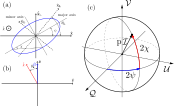
\includegraphics[width=\textwidth]{fig/tuneout/polz_diags}
	\caption{Aspects of light polarization in relation to the experiment. The polarization vector traces out an ellipse in the plane transverse to the light wavevector $\mathbf{k}$, depicted in (a). The ellipse traced in the plane normal to the propagation vector $\hat{k}$ is characterized by the angle $\psi$ between the major axis and the horizontal, and the angle $\chi$ determines the ellipticity (i.e. degree of circular polarization). The lab frame ($\hat{x}_L$) is rotated by an angle $\theta_L$ with respect to the atomic frame.  The light wave-vector is also potentially misaligned with the magnetic field vector, which defines the quantization axis of atomic angular momentum, as shown in (b). Such a possible misalignment factors into the transformation through the angle $\theta_k$. The polarization state can be treated as a real vector on the Poincar\'{e} sphere (c), on which the relationships between the elliptical angles are marked ($\chi$, the degree of circular polarization, gives the elevation angle in red. $\psi$ gives the polar angle, shown in blue). The position of the Stokes vector specifies a polarization state in terms of the Stokes parameters ($\st{Q,U,V}$), as described in the text. For example, circularly polarized light has an angle $\chi=\pi/4$ and thus an elevation angle $\pi/2$, thus living on the `north' or `south' poles of the Poincar\'{e} sphere ($|\st{V}|=1$). 
	}
	\label{fig:polz_figure}
	\end{figure}

	\subsubsection{Theory of polarized light}

	A monochromatic electric field takes on a classical state as
	\begin{equation}
		\vec{E}(\mathbf{r},t) = \mathcal{E}(\mathbf{r},t)\hat{\mathbf{u}}(\mathbf{r}),
		\label{eqn:lightfield}
	\end{equation}
	where $\hat{\mathbf{u}}$ is the unit polarization vector. The electric field propagates in the direction of the Poynting vector $\mathbf{S} = \mathbf{E}\times\mathbf{B}$, and hence we have $\hat{\mathbf{u}}\perp\mathbf{S}$ and $\hat{\mathbf{u}}\perp\vec{k}$, where $\vec{k}$ is the wave-vector of the light. Therefore, if we fix $z'$ as the propagation direction (i.e. along the beam axis, which we will relate the dashed coordinates to the lab frame shortly) then we can write the electric field in the coordinates $(x',y',z')$ as 
	\begin{equation}
		\vec{E}(\mathbf{r},t) = \begin{bmatrix}u_{x'}e^{i\phi_{x'}}\\
												u_{y'}e^{i\phi_{y'}}\\
												0
												\end{bmatrix}e^{i(kz'-2\pi f t)}.
	\end{equation}
	One can then consider the first two components, also known as the \emph{Jones vector} which captures the amplitude and relative phases in the $x'$ and $y'$ direction.
	We can write the Jones vector as a scalar multiplied by a unit-length vector $\hat{\mathbf{j}}$, and following a rotation by an angle $-\phi_x'$ we obtain
	\begin{align}
		\mathbf{j} &= |E|~\hat{\mathbf{j}}e^{-2\pi i f t},~\mathrm{where}\\
				\hat{\mathbf{j}}&= \begin{bmatrix}u_{x'}\\
								u_{y'}e^{i(\phi_{y'}-\phi_{x'})}\end{bmatrix}
	\end{align}
	and $u_{x'}={E_{x'}}/{|E|}$ (and similarly for $y'$).
	As the polarization vector precesses in time (as per the $t$-dependence in Eqn. \ref{eqn:lightfield}) it traces out a locus in the $x',y'$ plane normal to $\vec{k}$.
	For purely-polarized monochromatic light this locus is an ellipse, or rather the Lissajous figure whose $x'$ ($y'$) amplitude is given by $u_{x'}$ ($u_{y'}$) and the relative phase is $\phi_{y'}-\phi_{x'}$.
	Thus we have, for example, circularly polarized light when $u_{x'}=u_{y'}$ and $\phi_{y'}-\phi_{x'}=\pi/2$, or $\hat{\mathbf{j}} = (1,i)/\sqrt{2}$. On the other hand, if $\phi_{y'}-\phi_{x'}=0$ the light is linearly polarized along the axis given by $(u_{x'},u_{v'})$. 
	Up to a factor corresponding to the global phase, the Jones vector notation can be used to express the common polarization states of light in the following forms:

	
	\begin{minipage}{0.5\textwidth}
	\begin{align*}
	\mathbf{h} &= \begin{bmatrix}1\\0\end{bmatrix} \\
	\mathbf{d} =& \frac{1}{\sqrt{2}}\begin{bmatrix}1\\1\end{bmatrix} \\
	\mathbf{l} =& \frac{1}{\sqrt{2}}\begin{bmatrix}1\\i\end{bmatrix} 
	\end{align*}
	\end{minipage}
	\begin{minipage}{0.5\textwidth}
	\begin{align*}
		\mathbf{v} &= \begin{bmatrix}0\\1\end{bmatrix}\\
		\mathbf{a} =& \frac{1}{\sqrt{2}}\begin{bmatrix}1\\-1\end{bmatrix}\\
		\mathbf{r} =& \frac{1}{\sqrt{2}}\begin{bmatrix}1\\-i\end{bmatrix},
	\end{align*}
	\end{minipage}
	\hfill

	% \begin{tabular}{c c}
	% 	\centering
	% 	$\mathbf{h} = \begin{bmatrix}1\\0\end{bmatrix}$ & $\mathbf{v} = \begin{bmatrix}0\\1\end{bmatrix}$\\
	% 	&\\
	% 	$\mathbf{d} = \frac{1}{\sqrt{2}}\begin{bmatrix}1\\1\end{bmatrix}$ & $\mathbf{a} = \frac{1}{\sqrt{2}}\begin{bmatrix}1\\-1\end{bmatrix}$\\
	% 	&\\
	% 	$\mathbf{l} = \frac{1}{\sqrt{2}}\begin{bmatrix}1\\i\end{bmatrix}$ & $\mathbf{r} = \frac{1}{\sqrt{2}}\begin{bmatrix}1\\-i\end{bmatrix}$,
	% \end{tabular}
	% \end{table*}
	\noindent where the row-wise pairs correspond to the orthogonal pairs of horizontal/vertical, diagonal/antidiagonal, and left/right-circular polarization, respectively.
	Indeed any $\hat{\mathbf{j}}$ can be written as a linear combination of any row-wise pair of these vectors with complex coefficients.
	We can take a moment to notice that $\hat{\mathbf{j}}$ is a two-dimensional complex vector of length 1, and thus inhabits the same space as any two-level quantum system - i.e. a qubit.
	The coherence matrix\footnote{Elsewhere called the coherency matrix.} can thus be defined through the outer product
	\begin{align}
		\mathbf{\chi} &= \mathbf{j}^\dagger\otimes\mathbf{j} \\
		 &= \st{I} \begin{bmatrix} u_{x'}^2 & u_{x'} u_{y'} e^{-i(\phi_{x'}-\phi_{y'})} \\ u_{x'} u_{y'} e^{i(\phi_{x'}-\phi_{y'})} & u_{y'}^2\end{bmatrix},
	\end{align}
	where $I=|E|^2$ (which, up to some physical constants, is the intensity of the light field), and the off-diagonal elements are called the \emph{coherences}. 
	The outer product also maps the conventional polarization basis vectors to their respective matrix forms:

	\begin{minipage}{0.5\textwidth}
	\vspace{0pt}
	\begin{align*}
		{H} &= \begin{bmatrix}1&0\\0&0\end{bmatrix} \\
		{D} =& \frac{1}{{2}}\begin{bmatrix}1&1\\1&1\end{bmatrix}\\
		{L} =& \frac{1}{{2}}\begin{bmatrix}1&-i\\i&1\end{bmatrix}
	\end{align*}
	\end{minipage}
	\begin{minipage}{0.5\textwidth}
	\vspace{0pt}
	\begin{align*}
		{V} &= \begin{bmatrix}0&0\\0&1\end{bmatrix}\\
		{A} =& \frac{1}{{2}}\begin{bmatrix}1&-1\\-1&1\end{bmatrix}\\
		{R} =& \frac{1}{{2}}\begin{bmatrix}1&i\\-i&1\end{bmatrix}.
	\end{align*}
	\end{minipage}
	% \hfill

	% \begin{table*}[!h]
	% \centering
	% \begin{tabular}{c c}
	% 	${H} = \begin{bmatrix}1&0\\0&0\end{bmatrix}$ 					& ${V} = \begin{bmatrix}0&0\\0&1\end{bmatrix}$\\
	% 	&\\
	% 	${D} = \frac{1}{{2}}\begin{bmatrix}1&1\\1&1\end{bmatrix}$ &$ {A} = \frac{1}{{2}}\begin{bmatrix}1&-1\\-1&1\end{bmatrix}$\\
	% 	&\\
	% 	${L} = \frac{1}{{2}}\begin{bmatrix}1&-i\\i&1\end{bmatrix}$ & ${R} = \frac{1}{{2}}\begin{bmatrix}1&i\\-i&1\end{bmatrix}$.
	% \end{tabular}
	% \end{table*}
	
	The coherence matrix contains the full polarization information for a classical light-field and can be written in the Pauli basis as $\mathbf{\chi} = \sum_{i=0}^3 a_i\sigma^{i}$, where

	% \begin{table*}[!h]
	% \centering
	% \begin{tabular}
		% $\sigma_0 = \begin{bmatrix}1&0\\0&1\end{bmatrix}$, & $\sigma_1 = \begin{bmatrix}0&1\\1&0\end{bmatrix}$,\\
		% $\sigma_3 = \begin{bmatrix}0&-i\\i&0\end{bmatrix}$, and & $\sigma_3 = \begin{bmatrix}1&0\\0&-1\end{bmatrix}$.
	% \end{tabular}
	% \end{table*}

	\begin{minipage}{0.5\textwidth}
	\vspace{0pt}
	\begin{align*}
	\sigma_0 &= \begin{bmatrix}1&0\\0&1\end{bmatrix}\\
	\sigma_2 &= \begin{bmatrix}0&1\\1&0\end{bmatrix}
	\end{align*}
	\end{minipage}
	\hfill
	\begin{minipage}{0.5\textwidth}
	\vspace{0pt}
	\begin{align*}
		\sigma_1 &= \begin{bmatrix}1&0\\0&-1\end{bmatrix}\\
		\sigma_3 &= \begin{bmatrix}0&-i\\i&0\end{bmatrix}.
	\end{align*}
	\end{minipage}
	% \hfill


	% \begin{table*}[!h]
	% \centering
	% \begin{tabular}{c c}
	% 	$\sigma_0 = \begin{bmatrix}1&0\\0&1\end{bmatrix}$ 					&  $\sigma_1 = \begin{bmatrix}1&0\\0&-1\end{bmatrix}$\\
	% 	&\\
	% 	$\sigma_2 = \begin{bmatrix}0&1\\1&0\end{bmatrix}$ & $\sigma_3 = \begin{bmatrix}0&-i\\i&0\end{bmatrix}.$ \\
	% \end{tabular}
	% \end{table*}
	thus the coherence matrix can generally be written in the form $\chi = \frac{p\st{I}}{2}\left(\mb{1} + p\mathbf{s}\cdot\mathbf{\sigma}\right)$ where $\mathbf{s}=(\st{Q},\st{U},\st{V})\in\mathbb{R}^3$ and $|\mathbf{s}|=1$, analogous to the expression of a qubit state as a Bloch vector, where $\mb{1}=\sigma_0$ is the identity matrix\footnote{Note that the subscript indices differ from the Bloch sphere convention, opting instead for the convention consistent with the Stokes parameters.}.
	Note also that, as for the density matrix in the context of quantum states, the coherence matrix can be used to deal with statistical mixtures of polarization states. In this case, the purity $p\leq1$ can be introduced as a multiplying factor of the length of the (unit) Stokes vector $\mb{s}$. Fully incoherent light has $p=0$ and corresponds to the zero vector in the Stokes picture. Partially coherent light, for example an equal statistical mixture of $\mb{a}$ and $\mb{r}$, has a nonzero Stokes vector ($\frac{1}{2}(\mb{a}+\mb{r})=\frac{1}{2\sqrt{2}}(2,-(1+i))$) which lies inside the Poincar\'{e} sphere, while purely-polarized light lives on the surface of the sphere.
	
	By convention, the full form of the Stokes vector is $\mathbf{S} = (p\st{I},\st{Q},\st{U},\st{V})$ where $I$ corresponds to the beam intensity and the latter three components are the degrees of linear polarization ($\st{Q}$=$\pm$1 for horizontally and vertically polarized light), (anti-) diagonal polarization (accordingly, $\st{U}=\pm1$), and circular polarization (where we pick $\st{V}=\pm1$ for left- and right-circular polarization in the frame defined by the beam axis). Hereafter, we consider the case of purely-polarized light with $p=1$.
	Further, in the coherence matrix picture, the degree of polarization along vector $P$ (expressible as a linear combination of $\{H,V,D,A,R,L\}$) is given by the inner product Tr($\chi P$), as the algebra of the inner product is preserved under the linear action of the tensor product. 
	Completing the analogy, the pairs of orthogonal polarization are related by the transformation $\mathbf{s}\rightarrow-\mathbf{s}$ (just as orthogonal states of a qubit are at antipodal points on the Bloch sphere).
	
	The Stokes vector is illustrated on the Poincar\'{e} sphere, in relation to the polarization ellipse, in Fig. \ref{fig:polz_figure}.
	Notice that in taking the outer product, the factor $e^{\pm2\pi i f t}$ has vanished - the coherence matrix, just as for the density matrix, discards the global phase information by construction. 
	This can be a problem in applications concerning the coherent nature of laser light, wherein the Jones calculus is preferred for its preservation of phase information.
	However, in our case we are concerned with the time-averaged behaviour of the atom-light interaction (c.f. section \ref{sec:atoms_and_light}) and so this loss is not critical.
	For our treatment, we are considering purely polarized light in the experimental context of applying wave-plates after the output from a polarizing beamsplitter, and can do without this parameter.


\subsubsection*{Connection to experiment}
	\label{ssec:connection_to_experiment}

	A full definition of the Stokes parameters in terms of the unit electric field polarization vector $\mb{u}$ the $x',y'$ basis is:

	\begin{align}
	    \mathcal{I} &= |\mathbf{u}_{x'}|^2 + |\mathbf{u}_{y'}|^2 \\ 
	    \mathcal{Q} &= |\mathbf{u}_{x'}|^2 - |\mathbf{u}_{y'}|^2 \\
	    \mathcal{U} &= 2 \text{Re} \left(\mathbf{u}_{x'} \mathbf{u}_{y'}^*\right) \\
	    \mathcal{V} &= -2 \text{Im}\left(\mathbf{u}_{x'} \mathbf{u}_{y'}^*\right)
	\end{align}
	Which allows an expression in the form
	\begin{equation}
		\mathbf{S} = A \mathcal{J},
	\end{equation}
	where
	
	\begin{equation}
		A=\begin{bmatrix}
		 1 & 0 & 0 & 1 \\
		 1 & 0 & 0 & -1 \\
		 0 & 1 & 1 & 0 \\
		 0 & -i & i & 0 \\
		\end{bmatrix}
	\end{equation}
	and 
	
	\begin{align}
		\mathcal{J} &= \mathbf{j}^*\otimes\mathbf{j}\\
					&= (u_{x'}^2,u_{x'}u_{y'}e^{-i(\phi_{y'}-\phi_{x'})},u_{x'}u_{y'}e^{i(\phi_{y'}-\phi_{x'})},u_{y'}^2)^\mathrm{T},
	\end{align}
	Therefore the electric field components can be recovered, up to a global phase, via
	\begin{align}
		 \mathcal{J} &= A^{-1} \mathbf{S}\\
					 &= \frac{1}{2}\begin{bmatrix} 
					 				\st{I}+\st{Q}\\\st{U}+i\st{V}\\\st{U}-i\st{V}\\\st{I}-\st{Q}
								 	\end{bmatrix}.
	\end{align}
	thus the electric field components and their relative phase can be recovered through
	\begin{equation}
		 u_{x'} = \sqrt{\frac{\st{I}+\st{Q}}{2}},~u_{y'} = \sqrt{\frac{\st{I}-\st{Q}}{2}},~\phi_{y'}-\phi_{x'} = \mathrm{arctan}(\st{V}/\sqrt{1-\st{V}^2}),
	\end{equation}
	noting that, as expected, we are unable to retrieve the global phase information. For purely-polarized light, whose amplitude is obtained by $\sqrt{\st{I}}$, the real three-dimensional Stokes vector only contains enough parameters to specify the Jones vector. 
	However, we introduce the Stokes parameters for their utility in capturing the polarization-dependence of the atomic polarizability.


	We can now examine the $C$ and $D$ coefficients directly.
	Writing out the coefficient $C=2\mathrm{Im}(u_{x}^*u_y)$ we see it can be obtained by 
	\begin{equation}
	C=2\mathrm{Im}(u_{x}^*u_y) = -\mathrm{Tr}(\sigma_3\chi) = -\st{V}.
	\end{equation}
	That is, it gives the fourth stokes parameter, the degree of (right-) circular polarization in the atomic frame (indeed this follows directly from the definition of $\st{V}$).
	The $D$ coefficient can be seen to depend on the length of the polarization vector along the $z$ axis in the atomic frame, and can be shown \cite{Henson22} to depend on the second Stokes parameter $Q$ through
	\begin{equation}
		D = \frac{3}{2}\sin^2(\theta_k)(1+\st{Q}) - 1,
	\end{equation}
	where $\theta_k$ is the angle between the magnetic field pointing $\hat{b}$ and $\mathbf{k}$.
	The linearized tune-out equation thus reads
	\begin{align}
		 \fto = & \fto^S + \frac{\st{V}}{2}\beta^V - \frac{1}{2}\beta^T \left(\frac{3}{2}\sin^2(\theta_k)(1+\st{Q}) - 1\right)
		 \label{eqn:fto_stokes_eqn}
	\end{align}
	in terms of the Stokes parameters in the atomic reference frame. 

	% From which it follows that, in the case of purely-polarized light, one can write
	% \begin{equation}
	% 	\mathbf{j} = \frac{1}{\sqrt{2}}j (\iota + Q\mathbf{h}+V\mathbf{d}+V\mathbf{l}),
	% \end{equation}
	% where $\iota = (1,1)^\mathrm{T}$. 



\subsubsection{Magic wavelengths}
	% \rev{Similarly, `magic' wavelengths (where the light shift of a \emph{transition}, rather than a \emph{level}, cancels) have yielded absolute and relative determinations of DMEs \cite{Herold12,Leonard15}. However, calculations of these wavelengths are not currently competitive in accuracy with experiments \cite{Jasmeet17}, even for helium \cite{Zhang21}, whereas the tune-out wavelength of interest here is amenable to such a comparison.}
	It bears noting that tune-out points are associated with \emph{states} of the atom, where the stark shift $\Delta E_\mathrm{S} =0$.
	A distinct but related concept is `magic wavelengths' which are associated with \emph{transitions} between states and are defined by the point where the differential dynamic polarizability (or differential stark shift) vanishes: $\Delta E_\mathrm{S,U}-\Delta E_\mathrm{S,L} = 0$. 
	Magic wavelengths have attracted a great deal of interest for their utility in constructing optical lattice clocks \cite{Takamoto05,Derevianko11}, decoupling the clock transition frequency from the intensity of the trapping beams.
	% A major technical issue in atom- and ion-based frequency references is the calculation of the Stark shift due to black-body radiation from the vacuum chamber containing the test system \cite{Fasano21}.
	% Precision measurements of magic wavelengths constrain models of the polarizability over large spectral ranges and thus serve to characterize and help suppress black-body shifts in these systems \cite{Chanu20,Fasano21}.			
	% While magic wavelengths are presented by Nature to the scientist, it is also possible to emulate the effect of a magic wavelength by using an additional laser to counteract the Stark shift from a trapping or probe beam \cite{Hilton19}.
	% Recent progress has also overcome the higher-order effects beyond the electric dipole (namely the magnetic dipole, electric quadrupole, and hyperpolarizability effects) by precisely tuning the magic-wavelength trap to a `magic intensity' and achieving a Stark-shift cancellation to the $10^{-19}$  level in a Strontium latttice clock \cite{Ushijima18}.
	% Precision frequency measurements using neutral atoms (and ions \cite{Chanu20}) in optical lattices continue to provide constraints on possible variations in fundamental constants across space and time \cite{Uzan03,Blatt08,Huntemann14} and have been identified as compact detectors for gravitational waves \cite{Kolkowitz16} and dark matter candidates \cite{Derevianko14}.
	% Further, matter-wave guides built using magic wavelengths provide advantages for atom-interferometric gradiometry of gravitational and electromagnetic fields \cite{Akatsuka17}
	% Finally, magic (and indeed tune-out) wavelengths have recently been reported for ultracold diatomic molecules, thus extending the suite of control options available at the frontier of ultracold matter sciences \cite{Bause20}.


	Magic wavelengths are, of course, also of interest for their potential use in tests of basic atomic structure theory.
	However, most magic wavelength measurements to date have been made using heavy elements like strontium \cite{BilickiThesis}, barium \cite{Chanu20}, mercury \cite{Yi11}, rubidium \cite{Herold12}, and cesium \cite{Yoon19}, whose complex internal structure restricts the accuracy with which these wavelengths can be predicted.
	For instance, while current predictions of magic wavelengths in heavy elements are yet to reach parts-per-million precision, calculations for helium are already at this level \cite{Wu18,Zhang21_magic}.
	
	Highly precise measurements of magic wavelengths have been used to determine transition matrix elements in rubidium to a relative accuracy better than $10^{-3}$ \cite{Herold12}.
	For comparison, tune-out measurements in rubidium have yielded the ratio of oscillator strengths (rather than their absolute values) with accuracy at the $10^{-4}$ level \cite{Leonard15}.
	
	While the contribution of QED effects are included for helium magic wavelengths, their contribution is generally smaller than the theoretical uncertainty associated with the individual energy levels and thus are not yet ready for comparison with experiments.
	However, a very recent work identified the 1335 nm magic wavelength as a candidate for tests of atomic structure theory due to its sensitivity to the finite nuclear mass, and relativistic and QED effects \cite{Zhang21_magic} (contributing to the wavelength at the level of 232, 247, and 21 ppm respectively).
	A measurement of this wavelength to 0.01 nm precision (fractional error $\sim10^{-5}$) would suffice to check the predicted QED contributions.
	
	Indeed, magic wavelengths have already found use in tests of QED with helium, albeit through their role as dipole traps for precision measurements of forbidden transition energies \cite{Rengelink18}.
	A further application to helium was recently proposed wherein one would use a 1265 nm magic wavelength optical trap while another 934 nm magic wavelength beam provides the first of two photons for dichroic excitation of the forbidden $2\triplet S_1\rightarrow 3\triplet S_1$ transition near 427.7 nm \cite{Thomas20, Zhang21_forbidden}.
	This would reduce the effect of the main systematic uncertainty (the AC Stark shift) from 5 MHz to below 100 kHz.

	%% From Li-Yan's document (helium.pdf); the dynamic polarizability is $\alpha_1(\omega) = \sum_n \frac{f_{0n}}{\Delta E_{0n}^2 - \omega^2}$ in terms of all those oscillator strengths


	% \subsection{Other TO measurements}
	% 	\begin{itemize}
	% 	\item \todo{Read these past measurements}
	% 	\end{itemize}
	
	
	
	% As a test of QED, a tune-out frequency is advantageous because it is a null measurement, which does not require calibration of the light intensity or a measurement of excitation probability. These factors have previously limited the precision of direct transition strength measurements \cite{Boloufa09,Vogt07,Thomas20}. In comparison, previous tune-out measurements have been successful in measuring QED effects \cite{Leonard15,Holmgren12,Schmidt16,Herold12,Henson15}.
	% 2015 safranova theoretical identification of TO wavelengths in Strontium, check their accuracy
	% 	Ref for extracting transition rates
	% 	https://journals.aps.org/pra/abstract/10.1103/PhysRevA.92.040501

	% 2011 TOs for alkali metals, v early theory work
	% 	https://journals.aps.org/pra/abstract/10.1103/PhysRevA.84.043401
	% 2013 Cheng calculations of TOs for alkali-earth metals
	% 	https://journals.aps.org/pra/abstract/10.1103/PhysRevA.88.022511
	% 2013 Jiang prediction of TO wavelengths for potassium
	% 	https://journals.aps.org/pra/abstract/10.1103/PhysRevA.87.032518
	% 2016 Wang tune-outs in R, high precision measurements to 790.018187(193) and 790.032602(193) nm
	% 	Agree with theory (Leonard 15)
	% 	https://journals.aps.org/pra/abstract/10.1103/PhysRevA.94.052510
	% 2016 Schmidt 790nm tuneout in Rb by KD scattering of a BEC
	% 	790.01858(23) nm with sub-pm accuracy
	% 	https://journals.aps.org/pra/abstract/10.1103/PhysRevA.93.022507
	% 2016 Dammalapati calcs of magic and TOs for francium
	% 	https://journals.aps.org/pra/abstract/10.1103/PhysRevA.93.043407
	% 2017 Trubko Potassium TO 768.9701(4) nm using atom interferometry
	% 	 Ratio of oscillator strenghts inferred 2.066(11), ratio of line strenghts 1.9977(11)
	% 	https://journals.aps.org/pra/abstract/10.1103/PhysRevA.95.052507
	% 2017 Kao Dysprosium TO measurement, reported to the percent level, using kapitza-dirac diffraction
	% 	https://www.osapublishing.org/oe/fulltext.cfm?uri=oe-25-4-3411&id=359890 
	% 2017 Leonard high precision Rb tune-out measurement
	% 	erratum: Actual value = 790.032 326(32) nm, matrix element ratio 1.992 17(3)
	% 	theoretical value 790.0315(7) (after correction)

	% 2018 Tang predictions of Thallium TO and magics
	% 	https://journals.aps.org/pra/abstract/10.1103/PhysRevA.98.062511
	% 2019 Copenhaver 7Li tune-out measurement with atom interferometry
	% 	 3329.5(1.4) MHz for the tensor-shifted tune out  with σ± light polarization and 3310.6(4.9) MHz with scalar polz
	% 	 good ref for distinction between terms
	% 	https://journals.aps.org/pra/abstract/10.1103/PhysRevA.100.063603
	% 2020 Decamps 671nm TO for 7Li by atom interferometry
	% 	Can be corrected (via tensor terms) to agree with Copenhaver et al
	% 	https://journals.aps.org/pra/abstract/10.1103/PhysRevA.101.033614
	% 2020 Jian tune-out wavelength for 133Cs
	% 	Calculation - check precision, and note that tensor part is very very small in this case
	% 	https://journals.aps.org/pra/abstract/10.1103/PhysRevA.102.042823
	% 2021 Jiang tuneouts for Ba+ ions
	% 	Precision looks quite good
	% 	Sensitive to QED?
	% 	https://journals.aps.org/pra/abstract/10.1103/PhysRevA.103.032803
\subsection*{QED prediction of the tune-out point}
\label{sec:to_theory}
	% theory work
	Following the first prediction \cite{Mitroy13} and measurement  of the metastable helium  tune-out near 413 nm \cite{Henson15}, a vigorous campaign of theoretical studies \cite{Zhang16,ManaloThesis,Drake19,Zhang19, Pachucki19} has reduced the uncertainty in the predicted frequency, which previously limited comparison with experiment. In parallel with work at ANU, our collaborators\footnote{Namely Gordon Drake and Li-Yan Tang, with assistance from Aaron Bondy and Yong-Hui Zhang.} improved on the state-of-the-art calculation \cite{Zhang19} of the tune-out frequency.

	These calculations were performed using the non-relativistic QED method (nr-QED) and improve the precision by an order of magnitude (compared to the previous prediction \cite{Mitroy13}) with a total uncertainty at the level of 9 MHz (relative error $1.2\times10^{-8}$) . 
	The results are presented in Table~\ref{tab:theory} with a summary explanation here. A more detailed description is in the full manuscript \cite{Henson22}.
	
	\begin{table}[t]
	\centering
	%\vbox{\hsize 5.2in \noindent
	% \begin{ruledtabular}
	\begin{tabular}{l r r}
	\hline\hline
	Quantity    &Value (MHz) & Uncertainty (MHz) \\
	\hline
	\multicolumn{3}{c}{\textbf{Nonrelativistic and Relativistic terms}} \\
	Nonrelativistic (NR) & 725\,645\,115& 2       \\
	NR + relativistic scalar $(\alpha^{\rm S})$    & 725\,742\,216&6   \\
	Relativistic tensor $(-\frac12\alpha^{\rm T})$ &   1\,755& \\
	\hline
	Total non-QED        & 725\,743\,950&6     \\
	\hline
	\multicolumn{3}{c}{\textbf{QED terms}} \\
	QED $\alpha^3$       &       -7\,298& 1       \\
	QED $\alpha^4$       &          -127& 6       \\
	\hline
	Total QED            &         -7\,425& 8     \\
	\hline
	Retardation          &          -477 &        \\
	Nuclear size         &             5&          \\
	\hline
	Grand total          & 725\,736\,053& 9       \\
	Experiment           & 725\,736\,700& 260 \\
	\hline
	Difference           &          -647& 260\\
	\hline\hline
	\end{tabular}\\
	\caption{\label{tab:theory}Summary of theoretical contributions to the helium $\TO$ manifold tune-out frequency near 725.7 THz.}
	\label{tab:theory}
	% \end{ruledtabular}
	\end{table}

	The entries from nonrelativistic, relativistic, and QED contributions are not strictly additive because changing one effect, such as the relativistic correction, changes the tune-out frequency at which the other effects are evaluated.  Thus the first entry is the nonrelativistic tune-out frequency with finite nuclear mass effects included.  The next entry is the scalar part of the relativistic correction arising from the higher terms in the Breit interaction.  The entry from the spin-spin interaction (1755~MHz) is entirely responsible for the tensor part of the tune-out frequency (excluding the Schwinger radiative correction term $\alpha/\pi$).  These terms determine the nonrelativistic and relativistic part of the tune-out frequency.  The remaining terms are small enough that they can be added linearly.  The leading QED correction of order $\alpha^3$ ($-7298(6)$ MHz) includes the anomalous magnetic moment correction (8 MHz).  The terms of order $\alpha^4$ include only the radiative corrections.  The dominant source of uncertainty is thus the remaining nonradiative terms not included in the calculation, but which were previously computed for the $2^3S_1$ state energy \cite{Pachucki06}.  The remaining terms are the retardation correction of $-477$ MHz and a finite nuclear size correction.
	 % by accounting for finite nuclear size and mass, relativistic, QED, negative energy states, and finite wavelength retardation effects \cite{Drake19, Pachucki19,Henson22}. 
	% The interaction of an isolated atom with a freely propagating laser field is regarded as a zero in the coherent Rayleigh scattering cross section, rather than as a zero in the dynamic polarizability as is the case for an atom in an optical lattice. The two formulations are identical in lowest order, but not when retardation (finite wavelength) effects are taken into account. For convenience I will continue to use the $\alpha_(\omega)$ notation to denote a zero in the Rayleigh scattering cross section.

	% The nr-QED method considers the nonrelativistic Schr\"odinger equation and includes terms for the Breit interaction by perturbation theory \cite{BetheSalpeter,Piszczatowski15,Puchalski16,Puchalski20}.  The dynamic polarizability is expressed to second order in the interaction with a monochromatic oscillating electromagnetic field, and contributions from relativistic and QED effects enter through an additional perturbation.  
	% The included relativistic corrections are the spin-independent terms, the orbit-orbit interaction, the spin-dependent spin-spin interaction, and the Darwin term (see \cite{Henson22} for definitions and calculation of the aforementioned terms).
	% QED corrections are included in the form of effective operators up to fourth order in $\alpha$ \cite{Yerokhin10}, including the Araki-Sucher terms \cite{Araki57,Sucher58} ($\alpha^3$) and radiative QED terms ($\alpha^4$). The remaining nonradiative terms, amounting to about 5\% of the contributions from the radiative terms for the $2^3S_1$ state \cite{Piszczatowski15,Pachucki06}, result in an uncertainty of about 6MHz and are considered the dominant uncertainty.	A significant contribution of the theoretical work is the inclusion of retardation corrections recently derived by Pachucki and Puchalski \cite{Pachucki19,Drake19}.  These additions represent a reformulation of the problem as a zero in the coherent Rayleigh scattering amplitude for an atom in free space, instead of a zero in the frequency-dependent polarizability for an atom in an optical lattice \cite{Pachucki19,Drake19}. 






\section{Measurement technique}
\label{sec:trap_freq_measure}
	


	\begin{figure}
	\begin{minipage}{0.5\textwidth}
	\vspace{0pt}
	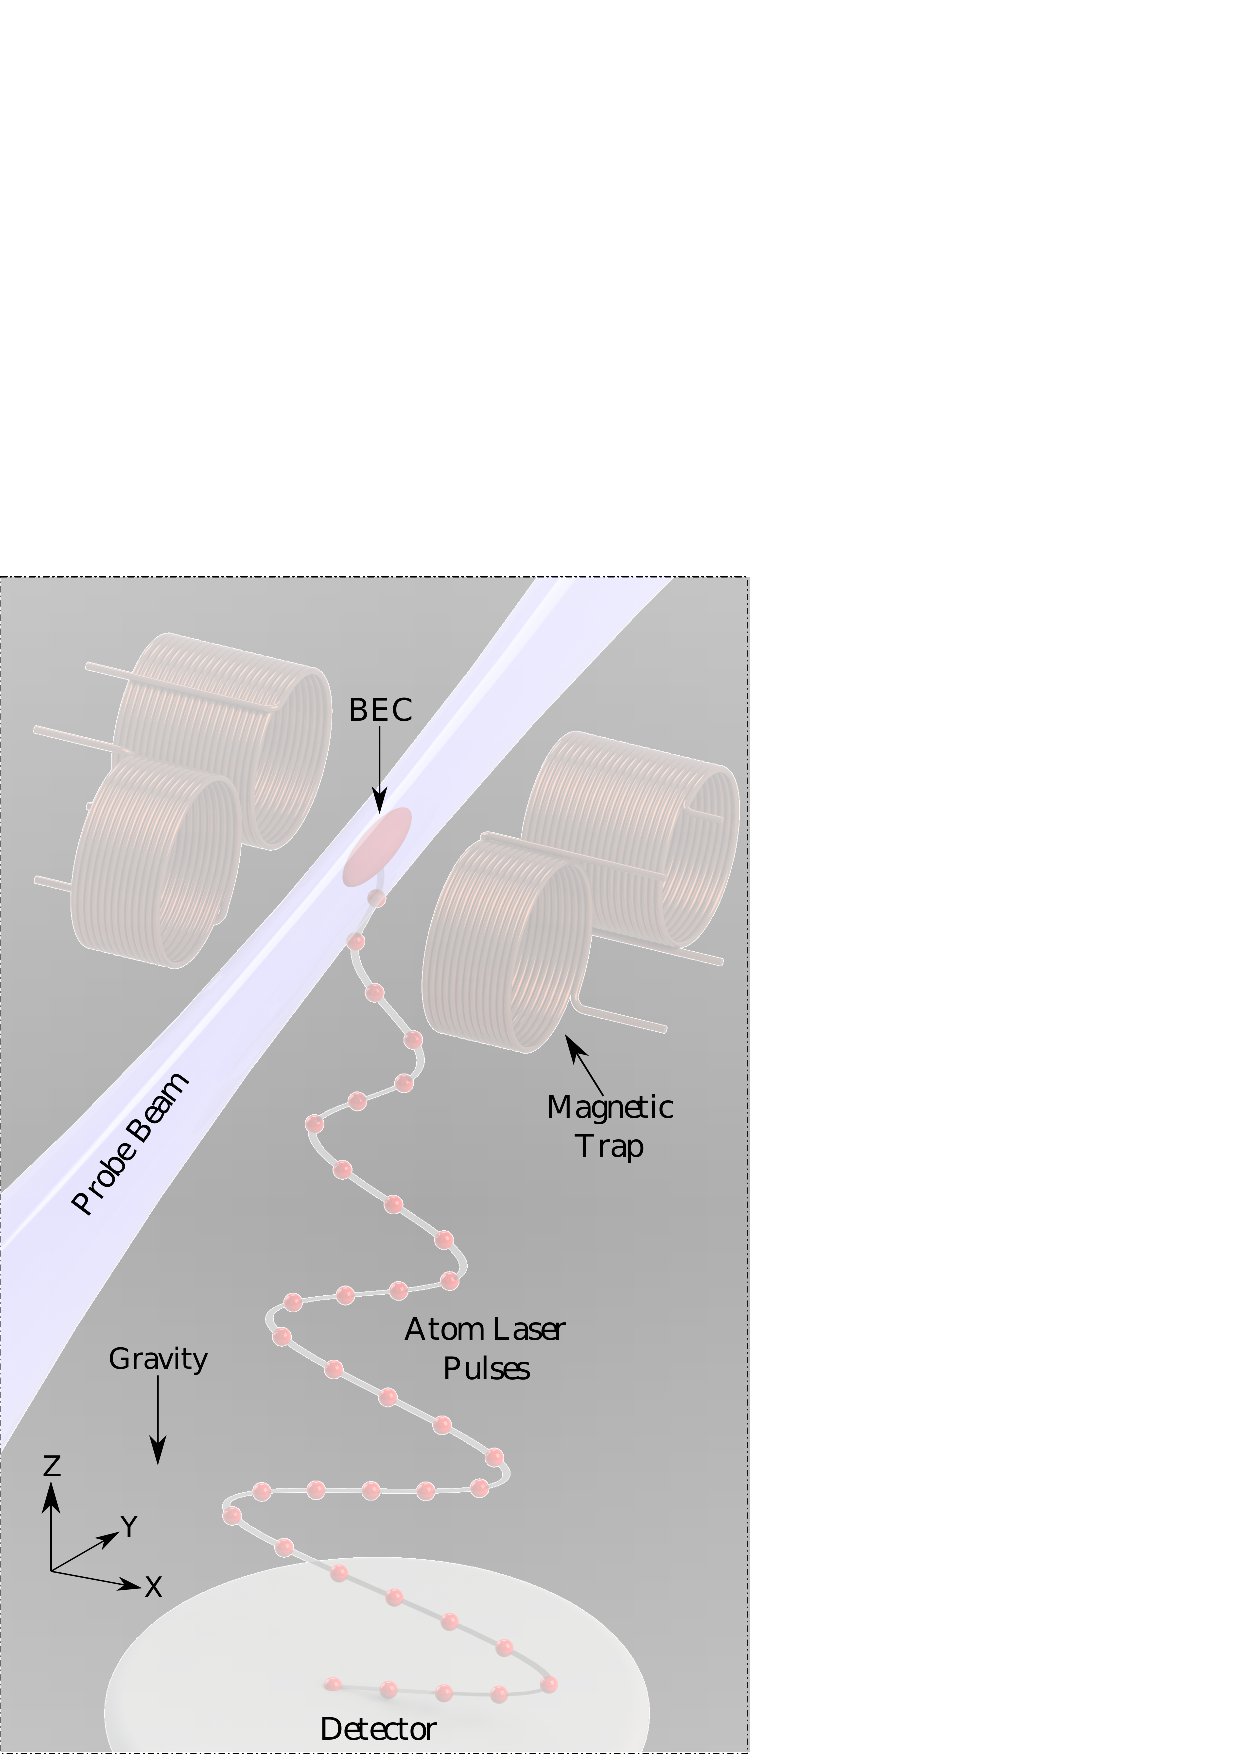
\includegraphics[width=\textwidth]{fig/tuneout/exp_schematic.png}
	\end{minipage}
	\hfill
	\begin{minipage}{0.5\textwidth}
	\vspace{0pt}
	\caption{
	Schematic of the physical system used to determine the tune-out frequency as a function of laser frequency. A magnetically trapped BEC of metastable helium atoms is illuminated with a probe laser beam with an adjustable (optical) frequency. The probe beam is aligned with the weak axis of the trap and oscillations are induced in the BEC centre of mass. The oscillation direction is horizontal and transverse to the laser beam, aligned with the axes of the BiQUIC coils.  A sequence of atom laser pulses (red spheres) is outcoupled from the BEC to sample the oscillation. The oscillation frequency is reconstructed by the anti-aliasing procedure described in section \ref{sec:trap_freq_meas}
	The lab-frame coordinate axes show the oscillation direction $y$, transverse to the beam axis $x$.
	}
	\label{fig:exp_schematic} 
	\end{minipage}
	\end{figure}

	Having defined a tune-out, we now turn our attention to the means we employed to determine the 413 nm tune-out using our apparatus. 
	This section provides a physical description of the measurement technique and establishes the important roles played by the frequency and polarization of the probe beam.
	To determine a tune-out point is essentially to measure the frequency where the optical dipole potential  vanishes.
	In our measurement, we quantified the shift in the oscillation frequency of a harmonically trapped BEC when the magnetic trap was overlapped with a power-stabilized probe laser beam (see Fig. \ref{fig:exp_schematic} and Section \ref{sec:spec_laser}). 
	This is in contrast to previous works (eg. \cite{Rengelink18}) wherein magic-wavelength optical traps were used in conjunction with a resonant probe beam. 
	The main motivations for the use of a magnetic trap are that it permits the pulsed outcoupling method, enabling the highly accurate trap frequency determinations which underpin this measurement. Furthermore, the magnetic field is easily configured to be extremely harmonic at length scales much larger than the BEC or its in-trap motion.

	The position-dependent potential energy in this hybrid trap is the sum of both the harmonic magnetic potential and a Gaussian optical potential,
	\begin{equation}
		U_\mathrm{net} = U_{\mathrm{trap}} + U_\mathrm{dip},
	\end{equation}
	where the magnetic trapping potential takes the form
	\begin{equation}
		U_\mathrm{trap} = \frac{m}{2}\left(\omega_{x}^{2}x^2+\omega_{y}^{2}y^2+\omega_{z}^{2}z^2 \right)
	\end{equation}
	where the $\omega_i$ terms are the oscillator frequencies of the harmonic magnetic trap, and the dipole potential is given in general by  \cite{Grimm00}
	\begin{align}
	    U_{\mathrm{dip}}=-\frac{1}{2 \epsilon_{0} c} \operatorname{Re}(\alpha) I(\rvec),
	\end{align}
	where $I(\rvec)$ is the local intensity of the electric field, $c$ is the speed of light and $\epsilon_0$ is the permittivity of free space.
	For a Gaussian beam which is aligned with the weak ($x$) axis of the trap and focuses $P$ watts of power to a spot size $w_0$, the intensity profile is 
	\begin{equation}
	    I_{\mathrm{dip}} =
	        \frac{2 P}{\pi w_0^2} \left(\frac{w_0}{w(x)}\right)^2 \exp\left( -\frac{1}{2} \frac{(y^2+z^2)}{w(x)^2} \right)
	 \end{equation}
	 where $w(x) = w_0\sqrt{1+(x/x_R)}$ is the waist size at a position $x$ along the beam axis and $x_R$ is the Rayleigh length. 
	 In the small-amplitude oscillation limit we can consider the total potential to be harmonic and retain only the terms up to second order in a Taylor expansion. If we further assume that the trapped BEC oscillates in the $y$ direction only then we can write the potential along the direction of motion as
	 \begin{equation}
	 U_\mathrm{net} \approx -\frac{\mathrm{Re}(\alpha)  P}{\pi 
   c {w_0}^2 \epsilon} + \left(\frac{2 \mathrm{Re}(\alpha)  P}{\pi  c {w_0}^4 \epsilon }+\frac{m {\omega_y}^2}{2}\right) y^2
	 \end{equation}
	 when evaluated about $x=z=0$.
	 Noting that the restoring force for a harmonic oscillator is given by $F_y = -\partial_y U_\mathrm{net} = -k_\mathrm{net} y$, we can identify the perturbed trapping frequency via the spring constant $k_y$:
	 \begin{align}
	 	\Omega_\mathrm{net} &= \frac{1}{2\pi}\sqrt{\frac{k_\mathrm{net}}{m}}\\
	 	&= \frac{1}{2\pi}\sqrt{{\omega_y}^2+\frac{4 P \mathrm{Re}(\alpha)}{\pi m c \epsilon w_{0}^4}}
	 \end{align}
	wherein we can identify the trap and probe frequency contributions by setting $P=0$ and $\omega_y=0$, respectively. 
	We thus obtain 
	\begin{equation}
		\Omega_\mathrm{probe} = \frac{1}{2\pi}\sqrt{\frac{4 \mathrm{Re}(\alpha)  P}{\pi m c \epsilon w_{0}^4}}
		\label{eqn:omega_probe}
	\end{equation}
	and have the relation
	\begin{align}
		\Omega_\mathrm{net}^2 &= \Omega_\mathrm{trap}^2 + \Omega_\mathrm{probe}^2\\
		&= \Omega_\mathrm{trap}^2 + \frac{4P}{\pi m c \epsilon w_{0}^4}\mathrm{Re}(\alpha)
		\label{eq:delta_omega_squared}
	\end{align}
	which shows that the squared shift in trapping frequency $\Omega_\mathrm{probe}^2 = \Omega_\mathrm{net}^2 - \Omega_\mathrm{trap}^2$ is linear in the probe power and the polarizability.
	Note the $\Omega$ terms have units 1/time - the trapping frequencies $\omega_i$ are angular frequencies with units Rad Hz. Thus, $\Omega_\textrm{trap} = \omega_y/2\pi$.
	
	\begin{figure}
	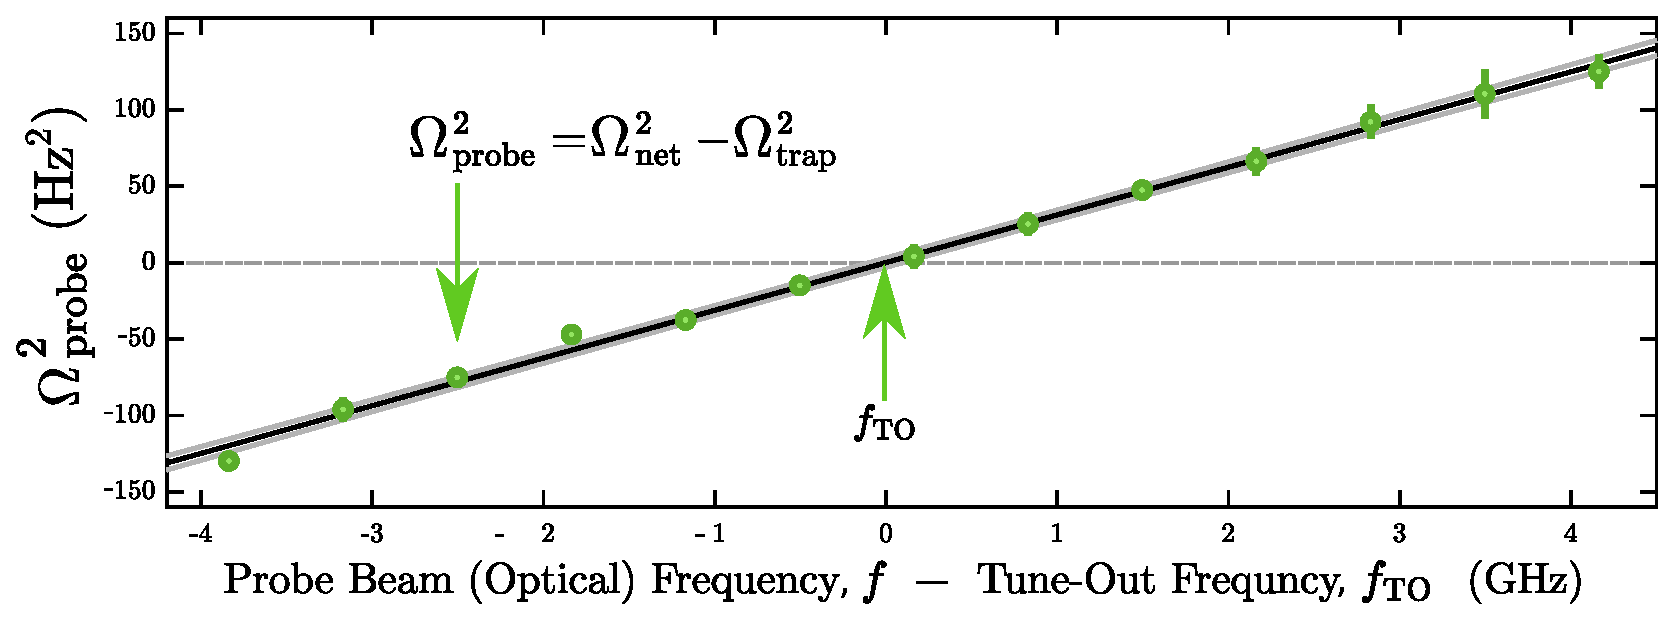
\includegraphics[width=\textwidth]{fig/tuneout/freq_scan}
	\caption{
	Determining the tune-out frequency for fixed polarization. The squared probe beam trap frequency (response) is found by comparison to a measurement of the unperturbed trap frequency. We repeated these measurements over a small frequency interval and extract the tune-out by finding the \textit{x}-intercept of the response. Also shown is the linear fit (black solid line) with light grey lines showing the \(1\sigma\) confidence intervals about the expected value of the mean. All error bars on points represent the standard error in the mean.
	}
	\label{fig:freq_scan} 
	\end{figure}

	An immediate corollary of Eqn. \ref{eq:delta_omega_squared} is that if the probe beam power is stabilized then $\Omega_\mathrm{probe}^2$	is linear solely in $\mathrm{Re}(\alpha)$. 
	It then follows that ascertaining the frequency at which $\Omega_\mathrm{probe}=0$ constitutes a determination of the tune-out point.
	Figure \ref{fig:freq_scan} shows the linear variation of experimentally-determined values of $\Omega_\mathrm{probe}^2$ versus the probe beam frequency $f$, demonstrating that this approximation holds in practise. 
	Indeed, we found that including a quadratic term in a fit to $\Omega_\mathrm{probe}^2(f)$ yielded an estimate of the zero-crossing frequency that was not statistically distinguishable from the zero-crossing estimate obtained from a linear fit.
	Section \ref{sec:implementation} provides more information about the experimental methods we used to obtain these measurements.





\subsection{Experimental implementation}
	\label{sec:implementation}
	We implemented such a hybrid trap using the BiQUIC machine and the tunable laser system described in chapter \ref{chap:apparatus}, especially section \ref{sec:spec_laser}. 
	The beam was tightly focused down to a waist of order 10 $\mu$m at the magnetic trap centre, then aligned with the weak axis of the harmonic magnetic trap as illustrated in Fig. \ref{fig:exp_schematic}.
	The laser system delivers up to 150 mW of power to the vacuum chamber when operating at the wavelengths relevant to this measurement. 
	We then scanned the laser wavelength $\pm4$ GHz about the tune-out in 13 steps ($\sim666.7$ MHz intervals), depicted in Fig. \ref{fig:freq_scan} .	
	This range is chosen in order to minimize the nonlinearities that are present when the optical potential is strong (see the discussion of systematic effects in section \ref{sec:systematic_effects}) while still presenting a sufficient signal-to-noise for interpolation of the linear response.
	
	For a given magnetic or hybrid (magnetic and optical) trap, the trap frequency can be determined by repeatedly sampling the momentum during a single shot using a pulsed atom laser. 
	The trap frequency measurement technique is discussed briefly in the next section, and in more detail in the next chapter (specifically section \ref{sec:n0_cal}). 
	First, I describe the experimental sequence used to realize the test conditions.
	Each measurement began with the production of a BEC of $(6\pm1)\times10^5$ \mhe~atoms\footnote{The variation in atom number reflects the range of atom numbers used in all runs. Generally the atom number in a given data collection run has a standard deviation of no more than 10\% of the mean.} cooled to $\sim80$ nK ($T/T_c\approx 0.1$) to reduce damping via coupling to the thermal part.
	Just prior to the frequency measurement we applied a 50~$\mu$s current pulse to a small coil near the BEC, inducing oscillation in the $y$-axis with initial amplitude (velocity) of $\approx30~\mu$m ($15$ mm/s).
	About 1\% of the atoms in the BEC were outcoupled every 8ms by a 5$\mu$s pulse of RF radiation (resonant with the trap centre at 1.7 MHz), creating a pulsed atom laser.
	The outcoupled atoms are in the $m_J=0$ state which is unaffected by magnetic fields, including the trap, and thereafter freely fall the 852~mm to the MCP-DLD (section \ref{sec:DLD}).
	From the time-of-flight data we reconstruct the initial velocity of each atom.
	The average velocity of atoms in a given pulse is an estimate of the centre-of-mass velocity of the BEC at the time the pulse was applied.
	The in-trap oscillation thus resolves as a variation in the centre-of-mass position on the detector, as shown in Fig. \ref{fig:trap_freq_eg}.
	The underlying trap frequency is then determined by means of the anti-aliasing technique described in the next section and in section \ref{sec:n0_cal}.
	Ultracold clouds below the condensation temperature were used because thermal clouds are more strongly damped in their oscillation, which is the dominant limitation for the precision of the trap frequency measurement described below (see e.g., \cite{Henson22_PAL}). 
	This is a major factor in the improved precision of this measurement over the previous one \cite{Henson15}, thus while thermal clouds can certainly be used, they would compromise the accuracy of the measurement.
	% We gradually increased the RF power during the pulses to maintain a good signal-to-noise ratio for later pulses, which would otherwise be hampered by the geometric decay of the pulse population.
	% A fit using a model of the form $y = A \exp(-t/\tau)\sin(\omega_\mathrm{net}+\phi)$ to 130 samples of the mean velocity (see fig \ref{}) thus determines the trap frequency to within 10~mHz in a single experimental cycle. 

\subsubsection{Measuring the trapping frequency}
	\label{sec:trap_freq_meas}

	The oscillation frequency can be determined by fitting a damped sine wave to the centre-of-mass velocity as a function of time, as shown in Fig. \ref{fig:trap_freq_eg}.
	The sampling rate of the pulsed atom laser is limited by the velocity width of the BEC in the vertical axis (\(\sim40\)~mm/s, which corresponds to a temporal width at the detector of \(\sim\)4~ms) along with the vertical oscillation amplitude. This presents a challenge for measuring the trap frequency as the oscillation is much faster than the sampling rate. 
	Thus the true oscillation frequency is \emph{aliased} to a frequency below the Nyquist frequency of the sampling (with an 8 ms period, the sampling rate is 125~Hz, and the Nyquist frequency is half this again, about 62 Hz).
	It is possible to reconstruct the true trapping frequency using an anti-aliasing technique which I describe in more detail in section \ref{sec:n0_cal}.
	We find that our magnetic trap is extremely stable, with characterisic frequencies of $(\omega_x,\omega_y,\omega_z)= 2\pi\times(55.4(3),426.6(1),428.41(4))$ Hz (where the values in brackets represent the standard deviation all measurements, which is larger than the typical variation within a single run).
	\begin{figure}
	\centering
		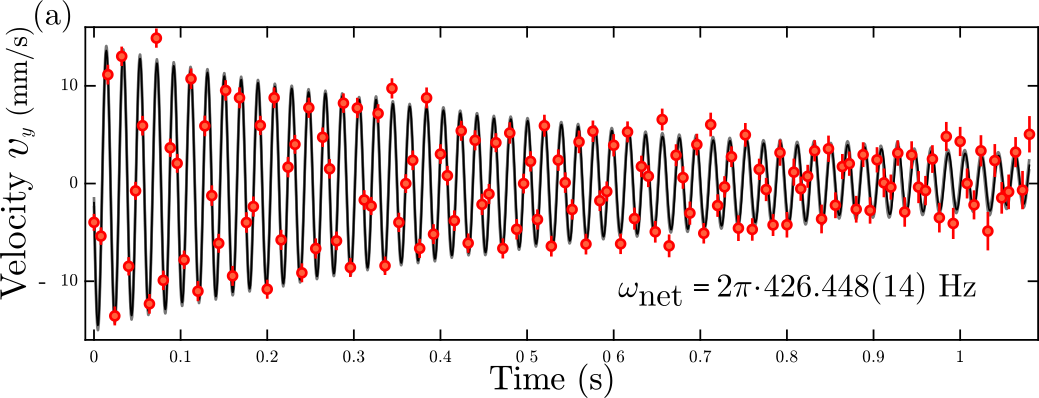
\includegraphics[width=0.8\textwidth]{fig/tuneout/trap_freq_eg}
			\caption{ Determining the trap frequency. The mean velocity of each pulse in the \textit{y}-direction ($v_y$) is used to trace out the oscillation over time (red points) and extract the oscillation frequency with a damped sine wave fit (solid line) for each realization of a BEC. The fitted frequency parameter is used to obtain the underlying trap frequency, as described in the surrounding text. A single experimental realization is shown.}
			\label{fig:trap_freq_eg}
	\end{figure}	
	
	The trap frequency measurement alternates between the combined trap and a purely magnetic trap to account for any drift in the magnetic trapping frequencies. 
	This calibration permits a determination of $\omega_\mathrm{probe}$ in two shots (about 50 seconds). 
	Given a measurement of the frequency $\omega_\mathrm{net}$ of the combined potential, the trap frequency $\omega_\mathrm{trap}$ (at the time of the interrogation) is predicted  by evaluating an interpolated model of the calibration frequency (smoothed by a Gaussian kernel with $\sigma=60$~s).
	This was done to correct for drifts of the magnetic trap frequency and to reduce noise. 
	The calibration data can also be used to obtain an estimate of the error in the trap frequency, which combines (true) trap frequency variation along with measurement error. 
	% We found that the underlying trap frequency had a standard deviation of 30 mHz across the longest data run, and that the overlapping Allan deviation at the 90s timescale (the smallest determinable given the experiment cycle time) was 18 mHz. 
	% These contribute fractional errors of 70 and 43 ppm, respectively.
	

		

	% To illustrate how we obtain the trapping frequencies, consider an undamped harmonic oscillator in one dimension. The centre-of-mass momentum $p(t) = A \cos(2\pi f t))$ oscillates at a frequency $f$ Hz, and the centre of mass of a pulse outcoupled at time $t'$ lands on the detector at a position $x'(t+\tau) = p(t')\tau/m$, where $\tau$ is the time of flight of the centre of mass. Sampling the cloud motion with a sampling period T starting at initial time $t_0$ produces a series of pulses whose centres of mass land at $\{x_n = (A\tau/m) \cos(\omega(t_0+nT))\}$. The sampling frequency $f_s=1/T$ determines the \emph{Nyquist frequency} $f_N=f_s/2$, which is the maximum frequency that can be reconstructed unambiguously from such a sampling regime. When $f>f_N$ the signal manifests as a lower-frequency oscillation known as the \emph{alias} of the signal. The aliased frequency $f_a$ is

	% \begin{equation}
	%  f_a =
	%   \begin{cases}
	%    \frac{Z_N f_s}{2} - f & \text{if } Z_N \text{ even} \\
	%    f - \frac{(Z_N-1)f_s}{2}       & \text{if } Z_N \text{ odd},
	%   \end{cases}
	%   \label{eqn:Z_N}
	% \end{equation}
	
	% where $Z_N = \lceil{f/f_N}\rceil$ is the Nyquist zone number, as described in numerous RF engineering references\footnote{Some good tutorials are presented \href{https://www.analog.com/media/en/training-seminars/tutorials/MT-002.pdf}{here} and \href{https://www.taborelec.com/Multi-Nyquist-Zones-Operation-Solution-Note}{here}.}. While it is not possible to determine $Z_N$ for a signal with an unknown (and not necessarily stationary) $f$ from samples taken at a fixed $f_s$, one can vary $f_s$ and determine both $Z_N$ and $f$.
	





% \subsection{


\subsubsection{Measuring polarization}

	% \newcommand{\Tr}[1]{\mathrm{Tr}}
	% The similarity between the Stokes and Bloch pictures extends even further indeed, permitting us to determine the Stokes parameters in the laboratory frame with simple measurements.
	% The action of a polarizing beamsplitter (PBS) introduces another degree of freedom which specifies the optical path.
	% For a $V$-transmitting PBS the (transmitted, reflected) intensities can be written as $\frac{1}{2}$(1+Tr($\sigma_1\chi$),1-Tr($\sigma_1\chi$)).
	We can measure the polarization of the light beam by use of a polarizing beamsplitter (PBS) and quater-wave plate.
	For our measurements we used a rotating Glan-Thompson polarizer with a high extinction ratio $>10^{5}$ in the transmitted component. 
	The calcite crystal in this type of polarizer internally reflects the $p$-polarized component (parallel to the \emph{plane of incidence} spanned by $\hat{k}$ and the normal to the optical surface) at the crystal interface, which leaves the $s$-polarized (parallel to the reflective surface) to exit through the transmitting port.
	That is, when the reflecting surface is vertical in the laboratory, the vertically-polarized component is transmitted, and the horizontally-polarized component is reflected.
	The fraction $p_T$ of optical power transmitted and reflected by the PBS are given by the projections $p_T=\Tr(\mathrm{V}\chi)=\frac{1-\st{Q}}{2}$ and $p_R=\Tr(\mathrm{H}\chi)=\frac{1+\st{Q}}{2}$, respectively. 
	Therefore one has $\st{Q} = \Tr(\sigma_1\chi) = p_R - p_T$. In terms of the absolute powers $P_T$ and $P_R$ measured at the beamsplitter ports, one must normalize by the total power and find 
	\begin{equation}
		p_R - p_T = \frac{P_R-P_T}{P_R+P_T}.
	\end{equation}
	which is commonly known as the \emph{contrast}.
	If one rotates the polarizer relative to the beam\footnote{This is usually much easier than rotating the lab relative to the polarizer.} by an angle $\theta$, this is equivalent to transforming the Stokes vector by matrix multiplication with
	\begin{equation}
		R(\theta) = \begin{bmatrix}
					1 & 0 & 0 & 0 \\
					0 & \cos(2\theta) & \sin(2\theta) & 0 \\
					0 & -\sin(2\theta) & \cos(2\theta) & 0 \\
					0 & 0 & 0 & 1
					\end{bmatrix}.
	\end{equation}
	The framework for considering the action of linear-optical elements by expressing them in such 4$\times$4 matrices which act on the Stokes vector is known as the Mueller calculus. Accordingly, the preceding matrix is (an example of) a Mueller matrix. 
	This allows a quantification of the observation that the maximum contrast occurs when the reflecting port of the polarizer is aligned (or orthogonal) with the major axis of the polarization ellipse.
	Denoting, then, the maximum and minimum transmitted powers, the maximum contrast (also called the \emph{visibility}) is $(P_\textrm{max}-P_\textrm{min})/(P_\textrm{max}+P_\textrm{min})$, where $P_\textrm{max}$ (resp. $P_\textrm{min}$) is the maximum (minimum) power transmitted over all polarizer angles $\theta$, which occurs when $\theta=\theta_\textrm{max}$ (resp. $\theta=\theta_\textrm{min}$). 
	Due to energy conservation considerations we should have $p_\textrm{max} = 1 - p_\textrm{min}$. 
	Further, if the major axis of the ellipse is at some angle $\theta_L$ from the laboratory $x$-axis, then the transmitted power will be minimized when the polarizer angle is at $\theta_L/2$ relative to the horizontal, c.f. the trigonometric terms in $R(\theta)$.
	Therefore we can obtain the laboratory $\st{Q}$ component via 
	\begin{equation}
		\mathcal{Q_{L}} =\frac{P_{\mathrm{max}}-P_{\mathrm{min}}}{P_{\mathrm{max}}+P_{\mathrm{min}}} \cos(2\theta_{\mathrm{min}}).
	\end{equation}
	We see also that the rotation matrix $R(\theta)$ does not mix the linear polarization components with $\st{V}$; the relative phases of the orthogonal oscillations are invariant.
	However, a similar argument to that just given can show that 
	\begin{equation}
		\mathcal{U_{L}} =\frac{P_{\mathrm{max}}-P_{\mathrm{min}}}{P_{\mathrm{max}}+P_{\mathrm{min}}} \sin(2\theta_{\mathrm{min}}),
	\end{equation}
	and so it follows from $|\mathbf{s}|=1$ that
	\begin{equation}
		\mathcal{V_{L}}^2 =\frac{4 P_\textrm{max}P_\textrm{min}}{(P_\textrm{max}P_\textrm{min})^2},
	\end{equation}
	which determines the degree, but not handedness, of the circular polarization in the lab frame.
	However, as we will see in section \ref{sec:fitting}, the sign of $\st{V}$ need not be determined directly as either sign can be made consistent with the tune-out equation within our analytical procedure.


	% In combination with a half- and quarter-wave plate pair, one can determine the polarization state of the light in a process similar to quantum state tomography of the qubit.
	% The general operator for a waveplate whose fast axis makes an angle $\theta$ with the horizontal, and which has a phase difference $\phi$ between the fast and slow axes, has the form
	% \begin{equation}
	% \mathrm{WP}(\theta,\phi)=\begin{bmatrix}
	% 						 1 & 0 & 0 & 0 \\
	% 						 0 & \cos ^2(2 \theta )+\cos (\phi ) \sin ^2(2 \theta ) & \cos (2 \theta ) (1-\cos (\phi )) \sin (2 \theta ) & \sin (2 \theta ) \sin (\phi ) \\
	% 						 0 & \cos (2 \theta ) (1-\cos (\phi )) \sin (2 \theta ) & \cos (\phi ) \cos ^2(2 \theta )+\sin ^2(2 \theta ) & -\cos (2 \theta ) \sin (\phi ) \\
	% 						 0 & -\sin (2 \theta ) \sin (\phi ) & \cos (2 \theta ) \sin (\phi ) & \cos (\phi ) 
	% \end{bmatrix}
	% \end{equation}
	% when acting on the (full) Stokes vector $\st(I,Q,U,V)$. This is an example of a Mueller matrix, which can also be constructed for other linear-optical elements. Note that the action of the operation is purely on the last three dimensions, leaving the purity and intensity unchanged.
	% A half-wave plate has $\phi=\pi/2$ and thus has an action of the form
	
	% \begin{equation}
	% \mathrm{HWP}(\theta)=\begin{bmatrix}
	% 					 1 & 0 & 0 & 0 \\
	% 					 0 & \cos ^2(2 \theta )-\sin ^2(2 \theta ) & 2 \cos (2 \theta ) \sin (2 \theta ) & 0 \\
	% 					 0 & 2 \cos (2 \theta ) \sin (2 \theta ) & \sin ^2(2 \theta )-\cos ^2(2 \theta ) & 0 \\
	% 					 0 & 0 & 0 & -1 
	% \end{bmatrix}
	% \end{equation}

	% while a quarter-wave plate has $\phi=\pi/4$ and thus has a Mueller matrix of the form

	% \begin{equation}
	% 	\mathrm{QWP}(\theta)=\begin{bmatrix}
	% 						 1 & 0 & 0 & 0 \\
	% 						 0 & \cos ^2(2 \theta ) & \cos (2 \theta ) \sin (2 \theta ) & \sin (2 \theta ) \\
	% 						 0 & \cos (2 \theta ) \sin (2 \theta ) & \sin ^2(2 \theta ) & -\cos (2 \theta ) \\
	% 						 0 & -\sin (2 \theta ) & \cos (2 \theta ) & 0.
 % 	\end{bmatrix}
	% \end{equation}
	% Thus the HWP can be seen to rotate the Stokes vector about the $\st{V}$ axis, while the QWP operation generates a more complicated action which mixes all three polarization components.

	% We employ the so-called power ratio technique to determine the probe beam polarization parameters \(\mathcal{V_{L}},\mathcal{Q_{L}}\) in the laboratory basis\footnote{}. The polarization parameters can be obtained by the relations
	% Define the contrast (the relative difference between either output port, also known as the visibility) as
	% \begin{equation}
	% 	p = \frac{p_{\mathrm{max}}-p_{\mathrm{min}}}{p_{\mathrm{max}}+p_{\mathrm{min}}}
	% \end{equation}
	% For a $V$-transmitting PBS the contrast is 1 for $H$, $V$, $D$, and $A$ light, depending on the angle of the polarizer relative to $u_x$.
	% Notice that if the polarizer is fully transmitting when the angle $\theta_
	% Rotating the polarizer 
	% The plane of polarization for linear light (including D and A light) can be determined by using a half-wave plate, which rotates the Jones vector 
	% If the light is in the any of the D, A, L, or R states, Tr($\sigma_1\chi$)=0 and thus the contrast will be zero.

	% \begin{align}
	%      \mathcal{Q_{L}} &=\frac{p_{\mathrm{max}}-p_{\mathrm{min}}}{p_{\mathrm{max}}+p_{\mathrm{min}}} \cos(2\theta_{\mathrm{min}}), \\
	%      |\mathcal{V}_{\mathcal{L}}| &= \frac{2\sqrt{p_{\mathrm{min}}p_{\mathrm{max}}}}{p_{\mathrm{min}}+p_{\mathrm{max}}},
	% \end{align}
	% where \(p_{\mathrm{max}}\) (\(+p_{\mathrm{min}}\)) is the maximum (minimum) power transmitted. The angle $\theta_{\mathrm{min}}$ is the angle (relative to the beam $x$-axis)  of rotation at which the polarizer transmission is minimized. The handedness of the circular component, which fixes the sign of $\mathcal{V_L}$, can be determined using a rotating quarter wave plate technique. 

\subsubsection*{Polarization at the atoms}

	% Ultimately what I want is to make the transformation $S_L \rightarrow E_L \rightarrow E_A \righarrow S_A$; begin with the Stokes parameters in the lab frame. Then, convert to the electric field representation and perform a coordinate transformation; then perform another transformation to the Stokes parameters in the new frame. 


	The transformation of $\mathcal{Q}$ from the laboratory to the atomic reference frame is given by a rotation around the probe beam axis by the angle \(\mathcal{\theta_{L}}\),
	and hence can be written in terms of the lab-measured parameters as
	\begin{equation}
	 \mathcal{Q_{A}} =\frac{P_{\mathrm{max}}-P_{\mathrm{min}}}{P_{\mathrm{max}}+P_{\mathrm{min}}} \cos(2(\mathcal{\theta_{L}}+\theta_{\mathrm{min}})).
	 \label{eqn:q_transform}
	\end{equation}
	This can also be interpreted as the rotation around the beam axis which aligns the laboratory polarizer angle origin with the component of the magnetic field vector which is orthogonal to $\mathbf{k}$. 
	Note that the circular component of the light is unchanged by the coordinate transformation, thus let us denote \(\mathcal{V_{L}}=\mathcal{V_{A}}\) by  \(\mathcal{V}\) hereafter.
	However, the rotation between the coordinate axes in the lab and atom frames mean that the Stokes parameters in the atomic frame are given by their respective projections, quantified in trigonometric coefficients.
	Thus, the final form of the tune-out equation is
	\begin{align}
		 \fto(\st{Q},\st{V}) = & \fto^S + \frac{\st{V}}{2}\cos{\theta_k}\beta^V - \frac{1}{2}\beta^T \left(\frac{3}{2}\sin^2(\theta_k)(1+\st{Q}) - 1\right)
		 \label{eqn:tune_out_eq}
	\end{align}
	where $\st{Q}=\st{Q_A}(\st{Q_L},\theta_L)$ in the atomic frame, as defined in Eqn. \ref{eqn:q_transform}. 
	The tune-out value $\fto(\st{Q}=-1,\st{V}=0)= \fto^S + \frac{1}{2}\beta^T$ is the sole option that eliminates any dependence on $\theta_k$, and we can leave $\theta_L$ as a fit parameter.

\section{Determination of the tune-out frequency}

	We obtain \(f_{\mathrm{TO}}(-1,0)\) through three stages of measurements. 
	First, as described above, we fix the probe beam polarization $(\mathcal{Q_A},\mathcal{V})$ and frequency $f$, and then measure the atomic polarizability via the squared shift of the centre-of-mass oscillation frequency of a BEC in the combined optical dipole and magnetic potentials ($\Omega_\mathrm{probe}^{2}(f)$).
	Second, we take many such measurements while scanning the probe beam frequency and find the optical frequency where the polarizability is zero for this probe beam polarization (i.e. the tune-out frequency \(f_{TO}(\mathcal{Q_A},\mathcal{V})\)) . 
	Finally, we measure $\fto(\mathcal{Q_A},\mathcal{V})$ for many settings of the probe beam polarization and extract \(f_{\mathrm{TO}}(-1,0)\) through the procedure described in this section. 
	

\label{sec:TO_analysis}

\subsection{Exclusion criteria}

	An experiment this complex is susceptible to many potential failure modes, and it is prudent for the experimentalist to mitigate against them.
	To ensure the integrity of the data set used for analysis we complemented the aforementioned control systems with a veto checklist in the data preprocessing pipeline.
	This consisted of a software screening procedure which discarded any measurements where any of the following essential conditions failed to hold. These conditions result in a loss of only one shot per $10^{4}$ across the whole dataset of 43500 shots. 



	\textbf{Single-mode laser:}	On rare occasions we observed that the Ti:S laser would spontaneously run in a mode where multiple optical frequencies were resonant in the cavity and present in the output, a so-called multi-mode regime (strictly a \emph{temporal} multi-mode regime, as distinct from the case where multiple spatial modes are present in the beam profile). This behaviour would cause the wavemeter to provide inaccurate frequency measurements, and also fail to produce the desired test conditions at the interaction zone. We eliminated runs where this happened by recording the output of a scanning Fabry-Perot cavity (Thorlabs SA200-5B). We scanned the cavity over twice its full free-spectral range in a sawtooth manner by scanning the voltage across a piezoelectric actuator, which modulates the cavity length, at frequency of 20 Hz. 
	We recorded the piezo and photodiode voltage during the interrogation and also in a $\sim0.2$~s period before and after.
	The multimode condition was triggered when the separation between peaks detected in the photodiode voltage were less than the free-spectral range, indicating the presence of multiple optical frequencies.
	To detect these peaks we processed the voltage recordings from the photodiode at the output of the cavity using a peak-detection algorithm. The threshold for detection was a peak height that was $1.5\times10^{-3}$ times the peak transmission intensity, which could distinguish spurious (multimode) peaks from electronic noise (all multimode conditions we  observed had peak intensities some orders of magnitude larger than this).

	\textbf{Stable probe power:}		We employ a check on the probe beam power as measured by a photodiode that monitors a sample of the beam just before it enters the experimental chamber, as shown in Fig.~\ref{fig:tunable_laser}. This ensures that the power feedback system is operating at set point in all measurements used in the analysis. Restrictive thresholds are set on the mean ($<0.02$ fractional difference to set point), standard deviation ($<0.05$ of set point) and maximum difference between the mean and the set point ($<0.03$ of set point) of the power during interrogation.

	\textbf{Stable probe frequency:}		The probe beam frequency at each measurement is taken to be the average optical frequency returned by the wavemeter during the interrogation. Shots were rejected if the frequency records in the lock loop's log file had a standard deviation greater than $3$~MHz or a range greater than $5$~MHz. These thresholds were based on our observations of typical locked performance, wherein the wavemeter reading displayed excursions from the mean that were smaller than the aforementioned ranges.

	\textbf{High atom number:}		Shots with very low atom number would lead to inaccurate determinations of the trapping frequency because the damped-sine fit would not be able to fit to many points. We mitigated this by screening out shots with less than $2\times10^{5}$ detected atoms. We found that the choice of threshold introduces a negligible systematic shift in the final tune-out determination, hence we could use shots with a wide range of atom numbers.


	In the end, it is likely that most of the failed shots would have been detected by the outlier-removal step in the fitting procedure, and thus it is plausible that these exclusion rules were of marginal benefit. However, we did not compare the results of running the analysis with and without the exclusion.

\subsection{Regressing the tune-out against polarization}
 \label{sec:fitting}
	
	% In order to make a definitive comparison between experiment and theory we seek a single quantity, but the working above shows that the tune-out is not uniquely defined.
	% Also, we cannot directly measure \(\mathcal{\theta_{L}}\) or $\theta_k$ with sufficient accuracy.
	% Fortunately we can address both of these issues by judiciously choosing the tune-out for a specific polarization state such that the dependence on these parameters vanishes, which I describe in this section. 
	
	We measured the tune-out frequency for 75 (\(\mathcal{Q_{L}},\mathcal{V}\)) pairs, comprising a total of $736$ tune-out measurements.
	We then fit the linearized model (Eq.~(\ref{eqn:tune_out_eq})) to the data, regressing $\fto$ against the measured $\mathcal{Q_{L}}$ and $\mathcal{V}$ values using five free parameters: $f^{S}_{TO}$ (the frequency at which the scalar polarizability $\alpha^S(f)=0$), the angle $\theta_{\mathcal{L}}$ between the lab and atomic reference frames, the angle $\theta_{k}$ between the beam propagation vector $\hat{k}$ and the magnetic field pointing, and the reduced vector- and tensor-polarizabilities $\beta^V$ and $\beta^T$ (see section \ref{sec:polz_linearization}).
	We can then predict a value for $\fto(-1,0)$, despite the lack of precise knowledge of the magnetic field pointing, by evaluating the resulting model at \(\mathcal{Q_{A}}=-1,\mathcal{V}=0\) to find \(f_{\mathrm{TO}}(-1,0)\). 
	The statistical error in the calculated \(f_{\mathrm{TO}}(-1,0)\) is determined with a bootstrapping technique\footnote{In the bootstrap method, one applies an analysis procedure on subsets of the data. The variance of the resulting findings provides an estimate of the sample variance, quantifying the statistical error in the fit to the entire data set. Source code is available at \cite{bryce_bootstrap_error_code}.}. 
	Figure \ref{fig:full_tune_out} displays the $\mathcal{Q_{A}}$ value calculated from the measured $\mathcal{Q_{L}}$ using the fitted $\theta_{\mathcal{L}}$. The measured \(f_{TO}\) is displayed as a function of $\mathcal{Q_{A}}$, $\mathcal{V}$. Figure ~\ref{fig:full_tune_out} also shows the tune-out calculated using polarization measurements taken before and after the vacuum chamber.
	In Fig. \ref{fig:pol_TO}, the measurements are displayed by interpolating the tune-out measurements to the one-dimensional subspaces defined by $\st{V}=0$ (a) and $\st{Q}=0$ (b).
	\begin{figure}
	    \centering
	    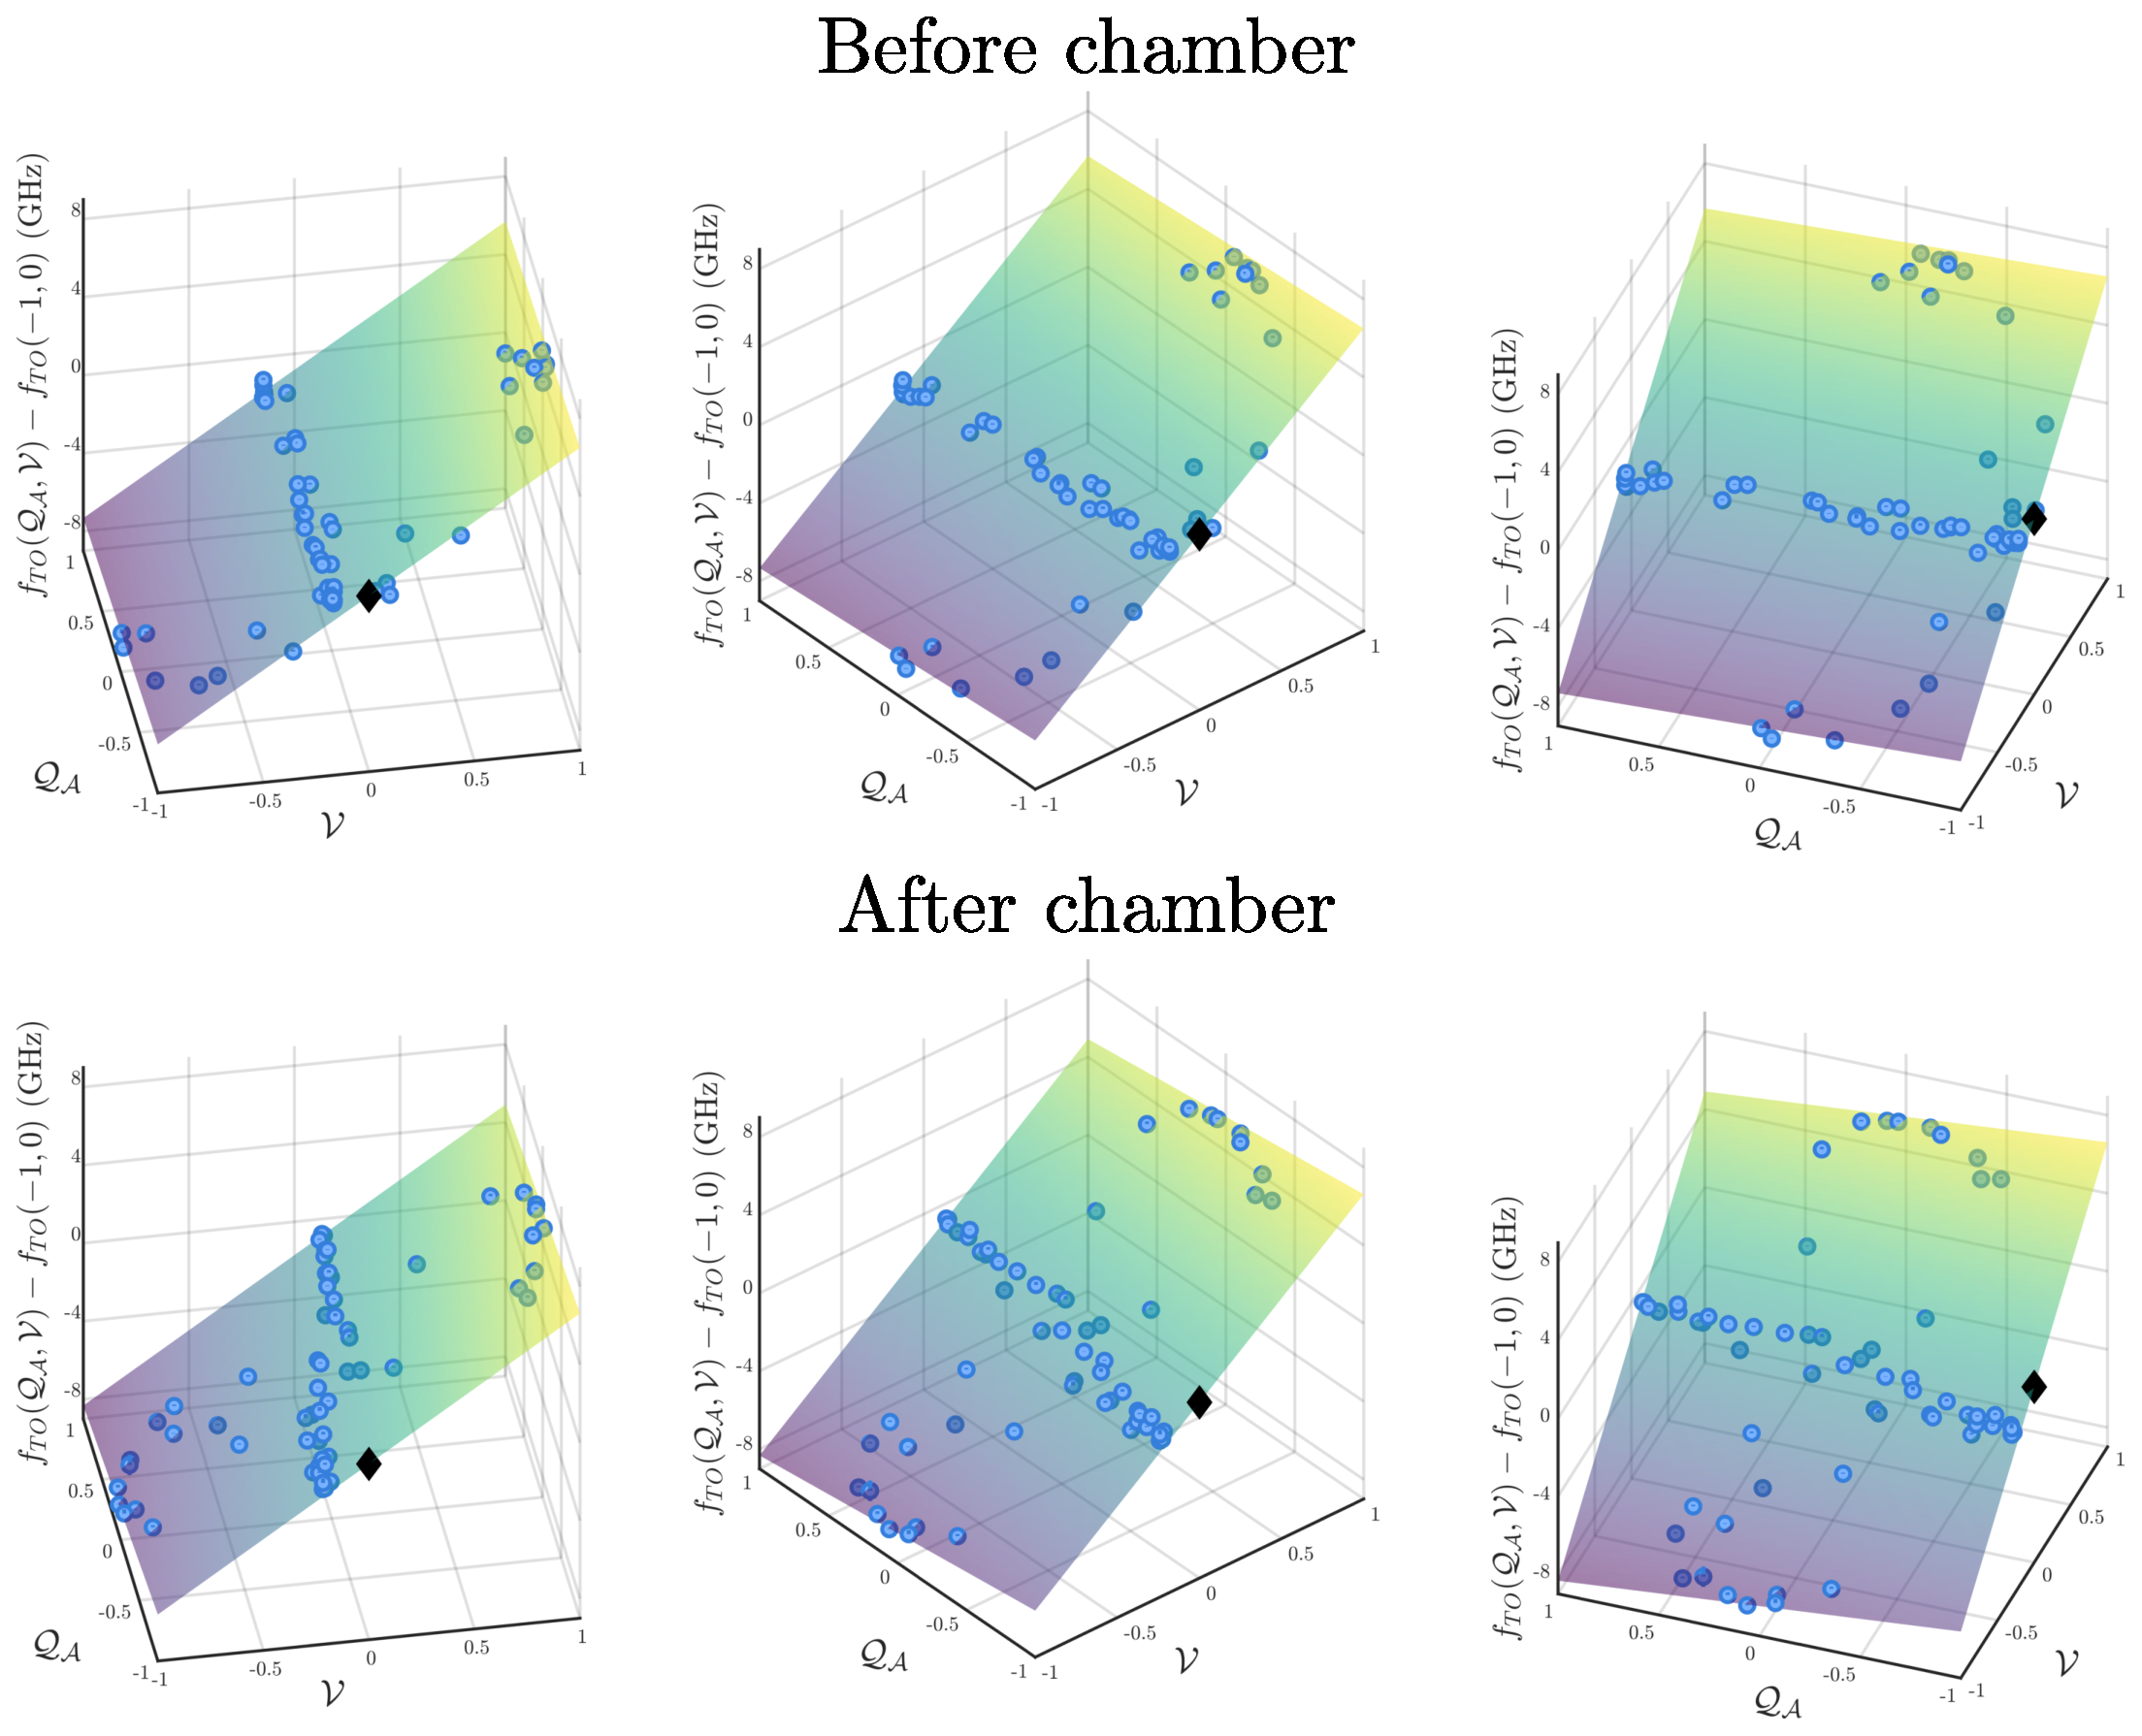
\includegraphics[width=\textwidth]{fig/tuneout/polz_pre_post}
	\caption{Visualizing the fit to $f_{TO}$ as a function of the polarization parameters $\mathcal{Q_{A}}$,\, $\mathcal{V}$  (see Eq.~(\ref{eqn:tune_out_eq})). The top row shows a fit using the polarization data taken before the vacuum chamber. The bottom row uses data taken after the vacuum chamber.  Each tuneout measurement is shown as a blue point. Note that (a-c) and (d-f) show, respectively, different viewing angles on the same data. The black diamond shows the value for \(f_{\mathrm{TO}}(-1,0)\) obtained in each case: \(f_{\mathrm{TO}}(-1,0)=725\, 736\, 810(40)\)~MHz in the top row, and \(f_{\mathrm{TO}}(-1,0)=725\, 736\, 610(40)\)~MHz in the bottom row. The other fit parameters are \(\beta^V \cos(\theta_k)=13240(70)\)~MHz, and \(\beta^T \sin^2(\theta_k)=1140(20)\)~MHz.}
	% top data:\(\beta^V \cos(\theta_k)=13240(70)\)~MHz, and \(\beta^T \sin^2(\theta_k)=1140(20)\)~MHz
	% bottom data: \(\beta^V \cos(\theta_k)=13012(100)\)~MHz, and \(\beta^T \sin^2(\theta_k)=550(100)\)~MHz
	\label{fig:full_tune_out}
	\end{figure}
	
	\begin{figure}
	\centering
	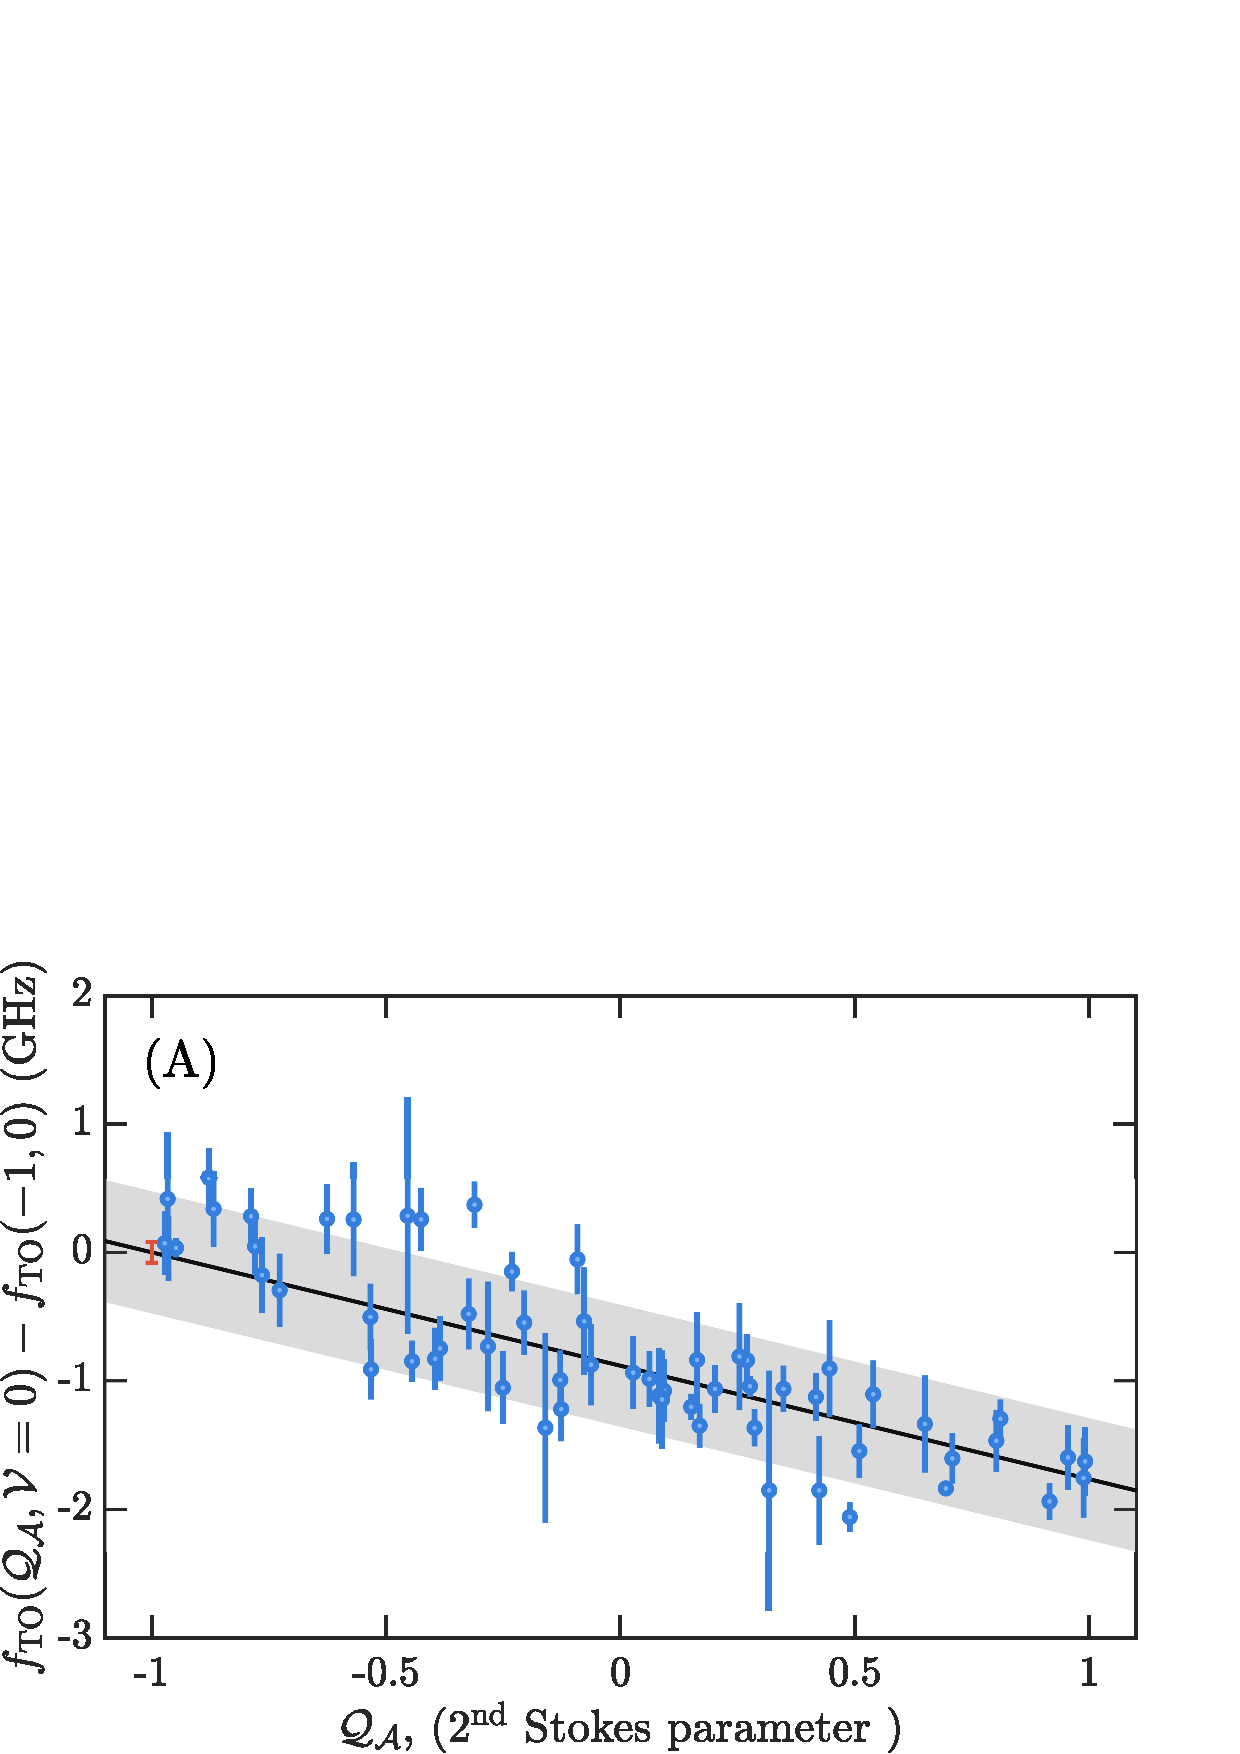
\includegraphics[width=\textwidth]{fig/tuneout/q_dep_1_min.pdf}
	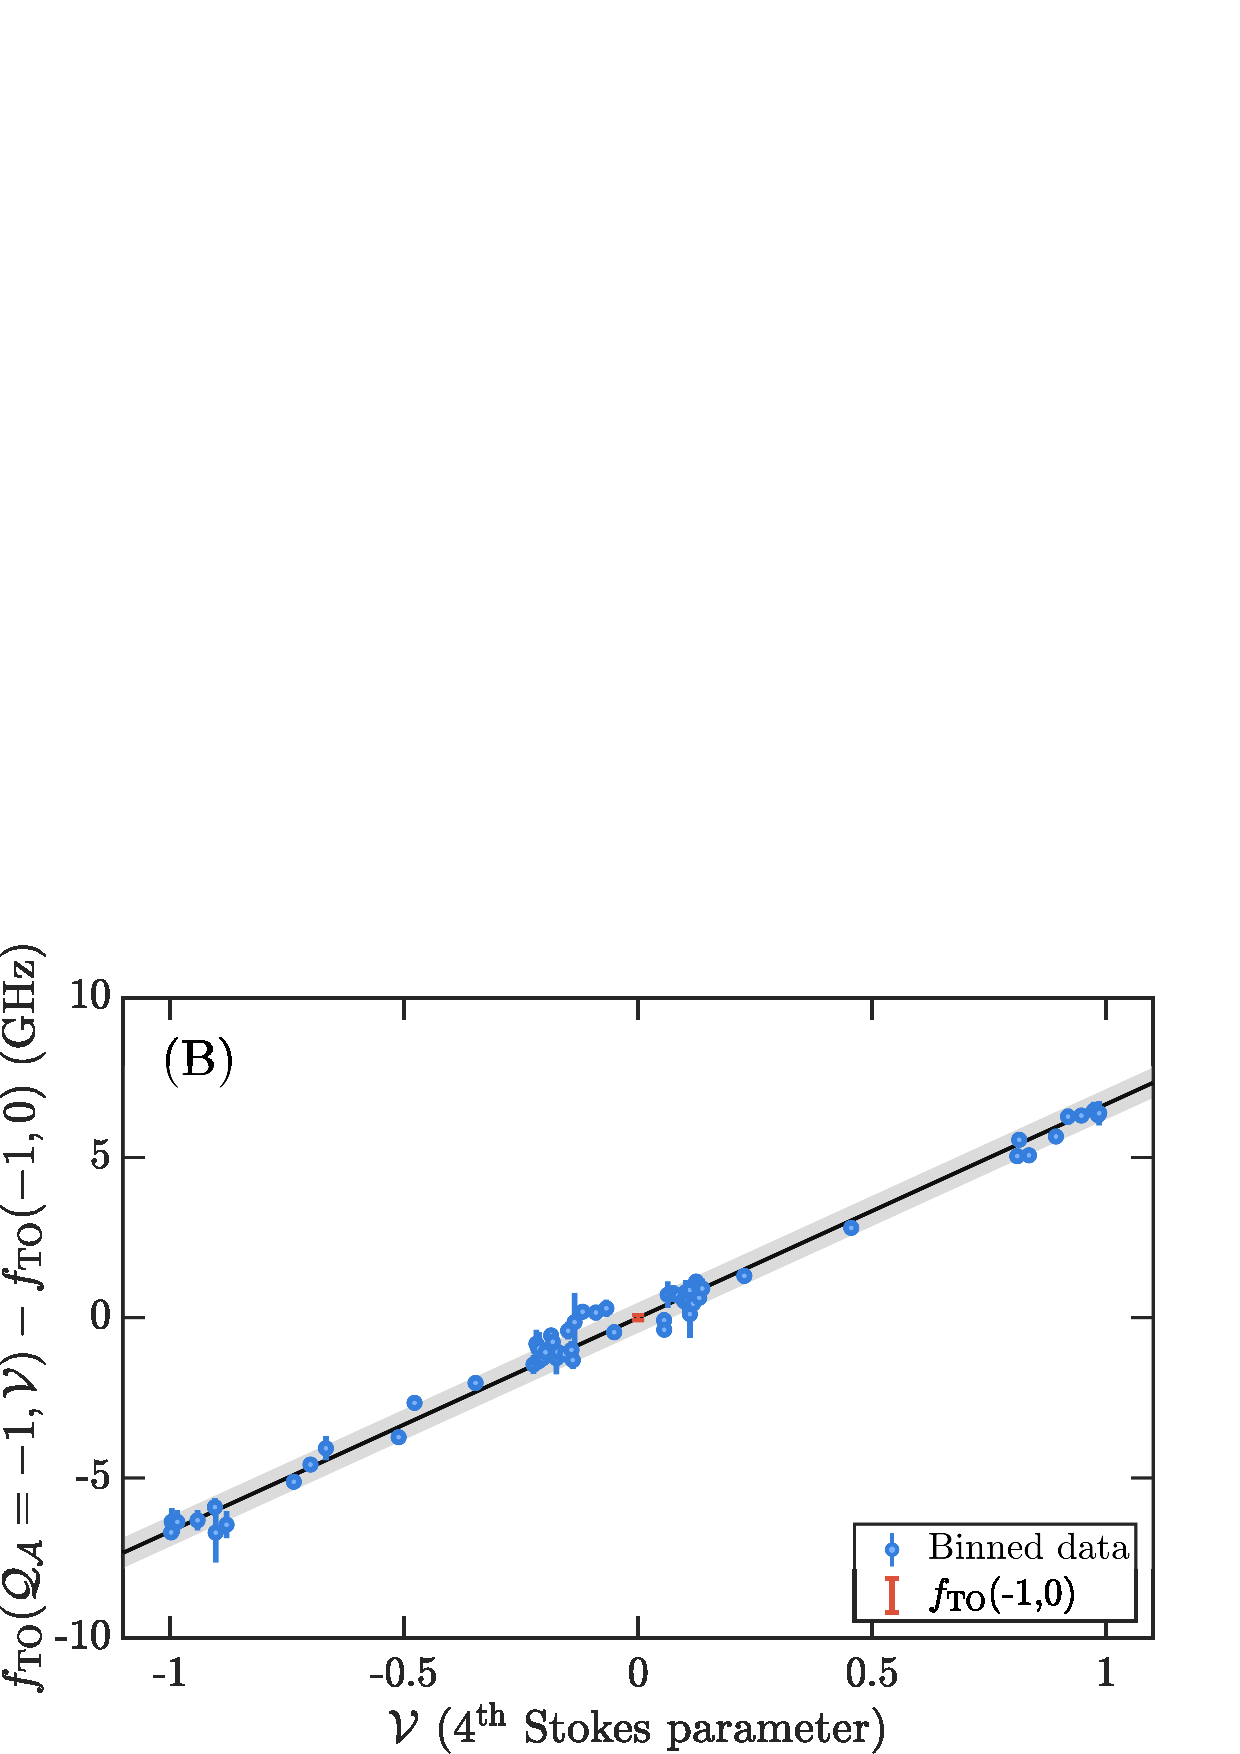
\includegraphics[width=\textwidth]{fig/tuneout/v_dep_1_min.pdf}
	\caption{
	Tune-out dependence on probe beam polarisation.
	% Evaluating the two-dimensional model along the one-dimensional sections defined by $\mathcal{V}=0$ (A) and $\mathcal{Q_{A}}=-1$ (B).
	 In (A), the data points show the $\omega_{TO}$ for each measurement after interpolating to the polarization state  ($\mathcal{Q_{A}},\mathcal{V}=0$). 
	Similarly, (B) shows the interpolation to  ($\mathcal{Q_{A}}=-1,\mathcal{V}$). 
	Error bars on the blue points are the estimated standard error in the mean value for a given polarization. The light-shaded and dark-shaded areas are the $1\sigma$ observation and confidence intervals, respectively. 
	The distinguished point is the predicted $\fto(-1,0)$, with the error bar indicating the (non-simultaneous) confidence interval.
	}
	\label{fig:pol_TO} 
	\end{figure}
	The preceding procedure amounts to finding the plane of best fit for trivariate data (i.e. triples of the form $(\st{Q},\st{V},f_{\mathrm{TO}}(\st{Q,V}))$), which requires only three parameters for complete specification. The use of five free parameters is an over-parametrization of the plane and thus the fit is overdetermined and cannot uniquely fix the fit parameters without additional measurements of at least one such quantity.	
	Further, the fit gives equal agreement between either polarity of \( \beta^T \), compensating by finding a different optimal value for $\theta_L$, and thus preventing a determination of \(f_{\mathrm{TO}}(-1,0)\). 
	To eliminate this issue, we constrain the sign of \( \beta^T \) using measurements and simulations of the magnetic field pointing and theoretical atomic structure calculations, both of which agree with the sign constraint \( \beta^T >0 \).
	We can also see here that the sign of $\st{V}$ is not critical; the cosine term can take on either sign, whereas the sine-squared term will be unchanged by a shift $\theta_k\mapsto\pi-\theta_k$.
	
	The presentation of the fit results in the remainder of this chapter include two distinct quantifications of statistical uncertainty intervals. The \emph{observation interval} quantifies the variance in data that is not explained by the predictor variables $\st{Q}$ and $\st{V}$ (\emph{i.e.} the noise around the mean value). This can also be interpreted as a measure of the expected variance of future observations at a given polarization value. In contrast, \emph{confidence intervals} quantify the uncertainty in the estimates of the model parameters. The  interval for a given confidence level $C$ denotes the range of values wherein a model parameter is expected to lie with a probability of $C$. 
	The confidence interval is similar to the standard error in that additional data can reduce the width of the confidence interval, whereas the observation interval quantifies the systematic variance and does not generally decrease with the addition of more data.
	The stated values for the fit parameters throughout this chapter are generally the 95\% confidence intervals, and when we predict the value of $f_\mathrm{TO}(-1,0)$, the relevant value is the mean value of tune-out measurements at this polarization value, and as such the relevant uncertainty interval is the confidence interval. The 1$\sigma$ observation interval ($C\approx 0.68$) is used to illustrate the variance of the data.

	The validity of the observation interval can be quantified by the reduced chi-squared ($\chi^2$) statistic, defined as follows.
	Given a model with input predictor- and outcome-data tuples $(x_i,y_i)$, the residuals are the difference $r_i=\hat{y}_i - y_i$ between the predicted value $\hat{y}_i$ and the true value. 
	If the estimated standard deviation of the model error (i.e. the 1$\sigma$ observation interval) is $\sigma_i$ (which may be defined at each $x_i$), then the chi-squared statistic is 
	\begin{equation}
	\chi^2 = \sum_i \left(\frac{r_i}{\sigma_i}\right)^2.
	\end{equation}
	The reduced chi-squared statistic is $\chi^2/d$, where $d$ is the number of error degrees of freedom (that is, the number of observations minus the number of fit parameters).
	If the model error estimates are accurate (and one has normally-distributed residuals) then the reduced chi-squared statistic, also written $\chi^2$/dof, will be close to 1.
	On the other hand, a $\chi^2$/dof much larger than 1 indicates the error term is too small or that the model is overfitted (i.e. underestimates the underlying noise); a $\chi^2$/dof less than 1 indicates the model error is too large. In both extreme cases, the model is unlikely to generalize well to new data, but when $\chi^2$/dof $\approx$1, the predictions are expected to be more reliable. The $\chi^2$/dof is given in figure captions where relevant.

	

	% \todo{The fit parameters are $f_{TO}(-1,0)=725\,736\,700\,(40)$~MHz, $\beta^V \cos(\theta_k)=13\,240\,(70)$~MHz, $\beta^T \sin^2(\theta_k)=1\,140\,(20)$~MHz (uncertainties represent only statistical uncertainty). }

	% Technically speaking the the filled areas around the trend line represent the 1$\sigma$ observation band and 1$\sigma$ confidence band - these concepts generalize the observation and confidence \emph{intervals} (which apply to point measurements on univariate data) to the case of multivariate data. I opt for uniform use of the term 'interval' rather than 'band' for simplicity, noting that the technically correct terminology should be clear from context.



	% \todo{Define also the chi squared stat}

	% Nonlin vs lin model:
	% pre window
	% - Predicted f_TO(-1,0): 725735619(-115,115) MHz
 %      - Using non-simultaneous prediction CI
 %    - Prediction interval: (-1167,1167) MHz
 %      - Using non-simultaneous prediction CI
 %    - Differs from prior method prediction 725736390 (47) by 771 MHz
 %    post
 %   - Predicted f_TO(-1,0): 725736868(-63,63) MHz
 %      - Using non-simultaneous prediction CI
 %    - Prediction interval: (-933,933) MHz
 %      - Using non-simultaneous prediction CI
 %    - Differs from prior method prediction 725736832 (31) by -36 MHz






	% \begin{figure}
	%     \centering
	%     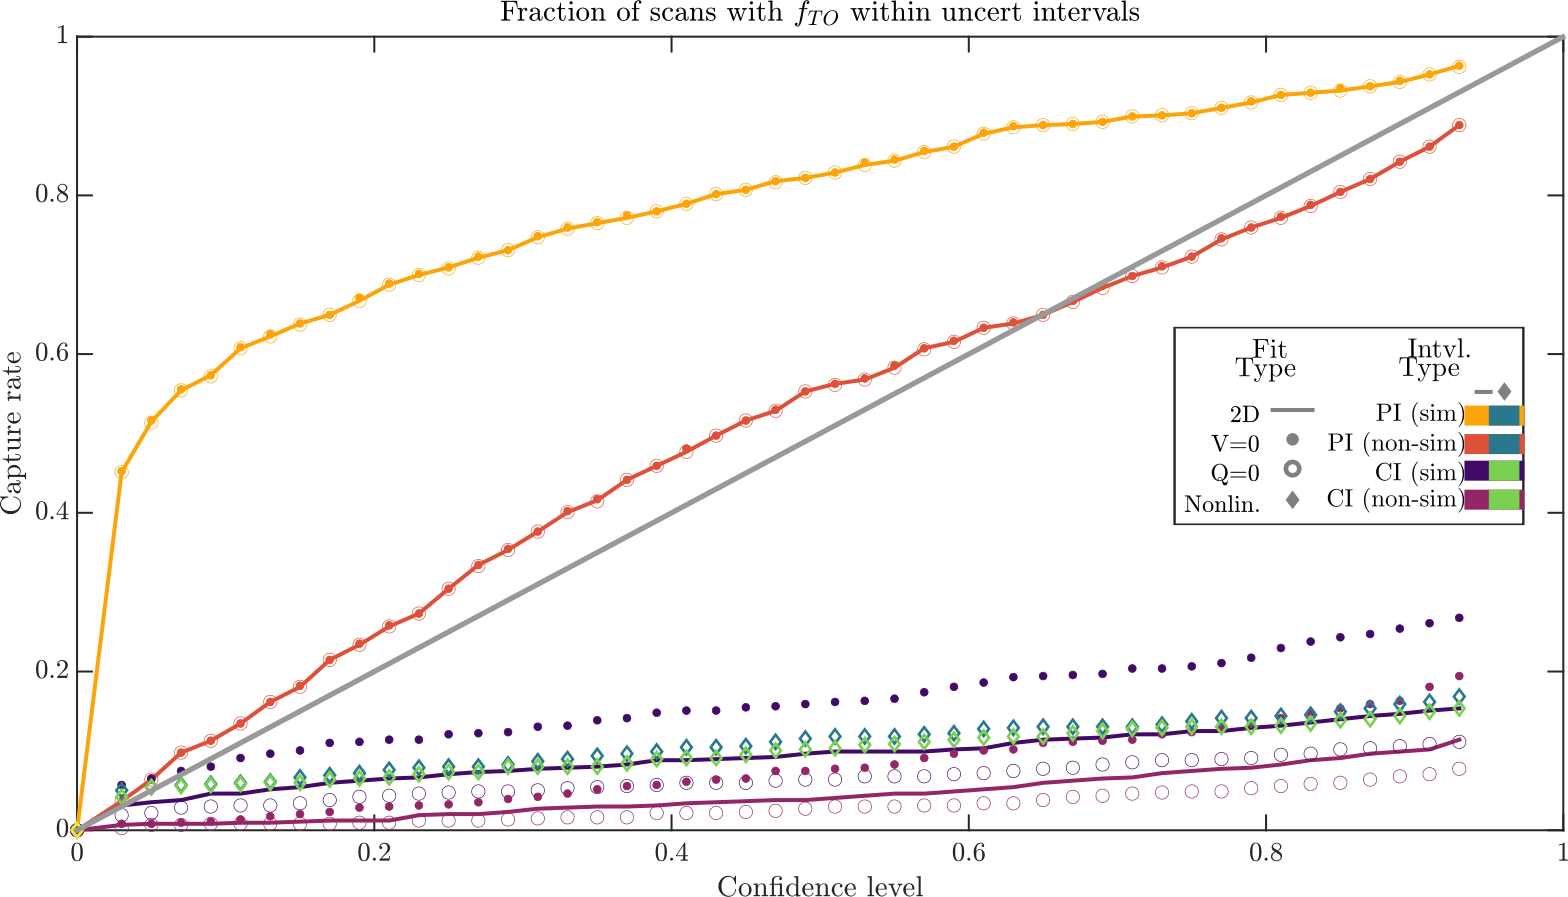
\includegraphics[width=\textwidth]{fig/tuneout/capture_rates}
	% \caption{Distinguishing variance from confidence with prediction bands.}
	% % top data:\(\beta^V \cos(\theta_k)=13240(70)\)~MHz, and \(\beta^T \sin^2(\theta_k)=1140(20)\)~MHz
	% % bottom data: \(\beta^V \cos(\theta_k)=13012(100)\)~MHz, and \(\beta^T \sin^2(\theta_k)=550(100)\)~MHz
	% \label{fig:full_tune_out}
	% \end{figure}


	% It is clear here that the estimated statistical error in the determined TO frequency for each scan is far less than spread between the the model and the data. (factor of 6 between SEWM of combined data and the sd of redisulas, will calc for each unbinned data pt) We attribute this to imperfections in the polarization measurement and variation of the magnetic field pointing.

	% The fit is weighted by the square of the uncertainty in each TO measurement $1/\sigma^2_{f_{TO}}$. The measured TO for each xx shot scan over wavelength for a given polarization is included in the fit as its own data point.
	% The fit is conducted with a global least squares prefitter that is constrained such that $-\pi/4<\theta_k<\pi/4$ and  $\beta^T>0$ which is then fed to an unconstrained fitter. 
	% In this way only a single parameter is required from theory, namely the sign of the tensor polarizability around the TO wavelength. This approach assumes that the tensor and vector polarization is approximately constant about the TO, consistent with theory [REF]\brycecom{from LYT}.

	% the frequency (wavelength) of light at which the atoms experience no perturbation is determined for some input probe polarization state and (ii) many of these measurement's (with varying degrees of circularity and linear orientation) are  combined and fit in Stokes space to determine the TO Scalar Minus Half Tensor (TOSMHT). The analysis for a given polarization state generally consists of hundreds of runs of the experiment grouped together to produce a measured TO for that polarization configuration.

	% and permits us to discern a peak potential energy of as little as 10$^{-35}$J. This is, to our knowledge, the smallest precision in a potential energy measurement reported to date \cite{Henson22}.  


\subsection{Validating linearity against theory}
 
We can use the values of the fit parameters to estimate the size of the polarization-dependent contributions to the measurement. That is, as a sanity check, we can make a low-precision comparison between theoretical predictions for the coefficients $\beta^V$ and $\beta^T$, and also compare the predicted and experimental value of the polarizability gradient $d\alpha/df$. These values are summarized in Tab. \ref{tab:param_compare} and the means by which we estimate them are given below. These values are not the primary interest of this work and accordingly we do not expect precise values to come from the experiment. However, we should expect that the range of values obtained from the experiment should at least include the theoretical prediction. 

%   - beta^V est 15070.4(-601.4,779.4)
%     - Theory val 12200.00
%     - Val ratio 1.24(-0.05,0.06)
%   - beta^T est 2635.0(-688.9,1201.3)
%     - Theory val 3400.00
%     - Val ratio 0.77(-0.20,0.35)


	First, we attend to an estimate of the gradient $d\alpha/df$, starting with its relation to the probe-beam induced shift $\Omega_\textrm{probe}^2$ in the (squared) trapping frequency (c.f. Eqn. \ref{eqn:omega_probe}),
	\begin{align}
	\frac{d~ Re(\alpha)}{d~f}&=A^{-1}\frac{d~\Omega_{\text{probe}}^2}{d~f},~\textrm{where}\\
	    A&=\frac{P}{m \epsilon_{0} c \pi^3  w_0^4}=\frac{1}{ \pi^2 m \epsilon_{0} c }\frac{I}{2 w_0^2}.
	    \label{eqn:da_df}
	\end{align}
	Figure \ref{fig:freq_scan} shows a response with a slope of approximately $d\Omega_\textrm{probe}^2/df \approx 30$ Hz$^2$/GHz, which is typical of the data collection runs. 
	We then need to compute the conversion factor, which in turn demands an estimate of the power and spot size of the laser beam at the interaction zone.
	We recorded of the probe beam power and profile obtained from measurements outside the vacuum chamber, but the vacuum window (through which the beam passes) subtly alters the beam profile and focal point.
	However, the arguments leading to Eqn. (\ref{eqn:omega_probe}) show that the tune-out is independent of the probe beam intensity (to first order) and therefore regular measurements of the beam profile were not necessary. 
	Hence, based on the measurements we did take of the profile through the course of the experiment, we adopt a conservative margin of error for the beam waist, using the range 15(5) $\mu$m. 
	Similarly we assume knowledge of the beam power at the trap to within about 20\%, i.e. $P\approx140(30)$ mW. The conversion factor $A=\frac{P}{m \epsilon_{0} c \pi^3  w_0^4}$ consistent with these values is $A\approx5(7)\times10^{45}$ kg A$^{-2}$  s$^{-6}$. 
	The uncertainty in this estimate is obtained by simple propagation of errors, and is dominated by the strong dependence on the beam waist that converts a 20\% error in $w_0$ into a $\sim140$\% uncertainty in $A$. 
	Note that Eqn. (\ref{eqn:da_df}) shows that the value $A$ must be positive if $d\Omega_{\textrm{Probe}}^2/df$ is positive (which it is in all shots included in the analysis), hence we can specify the uncertainty could be stated more strictly as $A=5^{+7}_{-5}\times10^{45}$.
	However, as this quantity is calculated for the purposes of a sanity-check, this detail is omitted from the remainder of the calculation.
	Thus the experimental value of the polarizability gradient is obtained by $d\Omega_{\textrm{Probe}}^2/df A^{-1}$ and has the value $5(7)\times10^{-54}~\textrm{C}~\textrm{m}^2~\textrm{V}^{-1}~\textrm{Hz}^{-1}$,
	 where the bracketed digit includes the statistical variation across all runs used in the analysis as well as the uncertainty due to imperfect knowledge of the beam parameters at the interrogation zone. 
	This value is included, with associated uncertainty interval, in Tab. \ref{tab:param_compare} and is broadly consistent with the theoretical value in that the theoretical value lies within the margins of error.
	The accuracy of this estimate is fundamentally limited by the quartic dependence on the beam waist, which was not precisely quantified as it is not a critical parameter for the purposes of measuring the tune-out frequency (Eqn. \ref{eqn:omega_probe} shows that the waist must only be stable, not precisely measured, to determine the tune-out frequency). However, as we discuss below in the context of the hyperpolarizability, the error induced by imperfect knowledge of the probe beam intensity is not significant.

	As for the polarization-dependent effects, our nonlinear fitting procedure returns $\beta^T\sin^2(\theta_k)=1140(20)$ MHz but, as noted above, unique values of $\beta^T$ and $\theta_k$ are not obtainable because the physical model is over-articulated (i.e. has more parameters than degrees of freedom due to physical constraints). 
	We can estimate the angle $\theta_k\approx 30^\circ$ from simulations of our magnetic trap, which is consistent with the fitted value of $25^\circ$. 
	Working with an estimate of $\theta_k = 27.5\pm(5)^\circ$, we determine the values shown in Tab. \ref{tab:param_compare}. 
	These calculations indicate effect sizes that are of the same order of magnitude as theoretical predictions, and whose uncertainty bounds also include the predicted value.
	Similarly, the theoretical value for $\beta^V$ is of comparable scale to the experimental value.
	The conclusion of the working in this section is that our linearized model for the tune-out is a good approximation for the system under relevant test conditions because our (approximate) inferences of relevant parameters agree with theoretical expectations.

	\begin{table}
	    \centering
	    \begin{tabular}{l c c c c c}
	        \hline\hline
	         Quantity & $d\alpha/df$ (C m$^2$ V$^{-1}$ Hz$^{-1}$) && $\beta^V$ (MHz) &&  $\beta^T$ (MHz)\\
	         \hline
	         Experiment & $5(7)\times10^{-54}$ &&  $1.5(1)\times10^4$ && $2.6^{+1.2}_{-0.6}\times10^3$\\
	         Theory & $1.78\times10^{-53}$ && $1.22\times10^4$ && $3.4\times10^3$\\
	         Ratio exp./thr. & 0.3(4) && 1.2(1) && \(0.8^{+0.4}_{-0.2}\)\\
	         \hline\hline
	    \end{tabular}
	    \caption{Comparison between the theoretical and experimentally-determined values for the gradient of the polarizability, and the reduced-vector and reduced-tensor polarizabilities. Note that the latter two are coupled via the fit model (through $\theta_k$) and hence this determination is not unique. Nonetheless, these comparisons show that the experimental values are generally consistent with the theoretical predictions. The parentheses denote the 1$\sigma$ uncertainty in the final digit. Uneven uncertainty intervals are quantified by the upper (superscript) and lower (subscript) values. All experimental values are within 2$\sigma$ of the predicted values.}
	    \label{tab:param_compare}
	\end{table}
\section{Systematic effects}
\label{sec:systematic_effects}

	
	

\subsection{Polarization}

	 The extraction of \(\fto(-1,0)\) needs an accurate determination of the probe beam polarization at the point of interaction with the atoms. 
	 As we did not have polarization optics mounted in vacuo, we inferred it from measurements outside the vacuum system. 
	 We estimated the contribution of two effects: the birefringence of the vacuum windows and the variation of polarization across the beam profile.
	 

\subsubsection{Birefringence}
	
	The polarization of the light may be altered as it passes through the final optical element: The glass window into the vacuum chamber.
	This means that the in-vacuum polarization may be different from the polarization set by the pre-insertion optics and measured prior to vacuum entry.
 	We estimated the size of this effect by measuring the probe beam polarization before it entered the vacuum system, and again after it exited through a second window\footnote{A portion of the probe beam escaped back through the in-vacuum mirror at the LVIS and then the insertion window for the horizontal trapping beam of the first MOT, making this possible.}.
 	We determined the error by running the $\fto(-1,0)$ analysis, as above, using both sets of polarization measurements (see Fig.~\ref{fig:full_tune_out}). 
 	We found that these values agreed within \(200\)~MHz, and hence used the average of the two as the final measured value and, and the difference is taken to be the uncertainty associated with the window birefringence. 

\subsubsection{Polarization across the beam}

	We also observed a small variation in the polarization across the transverse profile of the beam, as measured through a 1mm-diameter aperture.
	We determined that the mirrors in the pre-vacuum optics were the culprit.
	We characterized this by measuring polarization at several points across the beam.
	Using the polarization measured far from the beam axis produces a value of \(f_{\mathrm{TO}}(-1,0)\) that is up to \(400\)~MHz different from using the polarization at the beam center. 
	However, these contributions from differently-polarized light are weighted by their respective intensities, and accordingly the  weighted values produce a \(150\)~MHz uncertainty in $\fto$.

\subsection{Linearity} \label{sec:syst.subsec:lin}
	There are two instances in the preceding discussion where a linear approximation has been made in order to render the analysis tractable.
	Here I quantify the possible systematic shifts that could arise from these approximations.

\subsubsection{Linearity of the frequency shift}
	The first instance is the assumption that the perturbation $\Omega_\mathrm{probe}^2$ is linear with respect to the probe beam frequency, which leads to the use of linear regressions on the individual scans to obtain \(f_{\mathrm{TO}}(\st{Q,V})\).
	This is only approximately true: The polarizability is a nonlinear function of laser frequency at larger distances from $\fto$ (on the THz scale). 
	Nonetheless, quadratic (and higher) terms included in the fits to the laser scans were not significant.
	Using a theoretical model of the polarizability, we found that a linear fit spanning 4~GHz either side of the tune-out would return a zero-crossing only $-88(1)$~kHz from the true tune-out. 
	If we were to measure out 40 GHz either side of the tune-out, this shift would increase to $-9.6(2)$~MHz because the quadratic (and higher-order) terms become more significant, reducing the accuracy of the linear fit.
	However, these shifts are reduced to 0.6~kHz and 40~kHz in the 4~GHz and 40~GHz cases, respectively, by including a quadratic term.
	In comparison to the other systematic effects, this linearization introduces a negligible error.

	% Our analysis to obtain \(f_{\mathrm{TO}}(-1,0)\) assumes the perturbation $\Omega_\mathrm{probe}^2$ is linear with respect to the probe beam frequency. 
\subsubsection{Linearity of hybrid potential}
	We also made a linear approximation when deriving the relation $\Omega_{\text{net}}^2=\Omega_{\text{trap}}^2+\Omega_{\text{probe}}^2$, which was derived assuming the probe beam created a harmonic potential, ignoring higher-order derivatives of the Gaussian optical potential.
	The overlapping combination of harmonic traps is also harmonic, thus the equations of motion of an oscillating BEC are given by linear second-order ODEs.
	In contrast, a feature of oscillatory motion in anharmonic potentials is that the period of oscillation depends on the total energy (\emph{i.e.} on the amplitude).
	We checked for this by fitting the damped-sine model to different (contiguous) subsets of the atom laser pulses.
	While we did observe that the largest oscillations were 0.3 Hz slower than the smallest, there was no discernable effect on the zero crossing $\fto$.  
	Hence, again, this was found to be a suitable approximation.


\subsubsection{Linearity in the beam intensity}
	
	We measured \(\Omega_{\mathrm{probe}}\) as a function of probe beam power, with the polarization and frequency fixed, to constrain any shift with respect to probe beam intensity. A second-degree polynomial was sufficient to describe the response, illustrated in Fig.~\ref{fig:probe_beam_linearity}. 
	We deduced that using a linear fit at experimentally-relevant beam powers, rather than a quadratic fit, would lead to a  \(-24(30)\)~MHz change in the determined tune-out.

		\begin{figure}
	    \begin{minipage}{0.58\textwidth}
	    \vspace{0pt}
	    \includegraphics[width=\textwidth]{fig/tuneout/probe_beam_linearity}
	    \end{minipage}
	    \hfill
	    \begin{minipage}{0.4\textwidth}
	    \vspace{0pt}
	    \caption{Testing for nonlinear response versus power. We set the  probe frequency 20~GHz blue of $\fto$,  producing a strong potential, and fit the response against the laser power P with the model \( \Omega_{\mathrm{probe}}^2 = a  P - b P^2 \).  The fit parameters are \(a=\text{30.3(1)}\times 10^{-3}\text{~Hz}^2\text{W}^{-1}\), \(b= \text{0.06(2)} \times 10^{-6}\text{~Hz}^2\text{W}^{-2}\), and $\chi^2$/dof=0.992. Higher-order terms  were not statistically significant. The \(1\sigma\) (observation) confidence interval is shaded. 	    }
	    \label{fig:probe_beam_linearity}
	    \end{minipage}
	\end{figure}



\subsection{Hyperpolarizability}

	The working above also assumes that the metastable-state energy shift due to a nonzero polarizability is a linear function of the light field intensity. 
	We combined theoretical predictions and experimental measurements to obtain an estimate for this error.
	

	\begin{figure}[t]
	    \centering
	    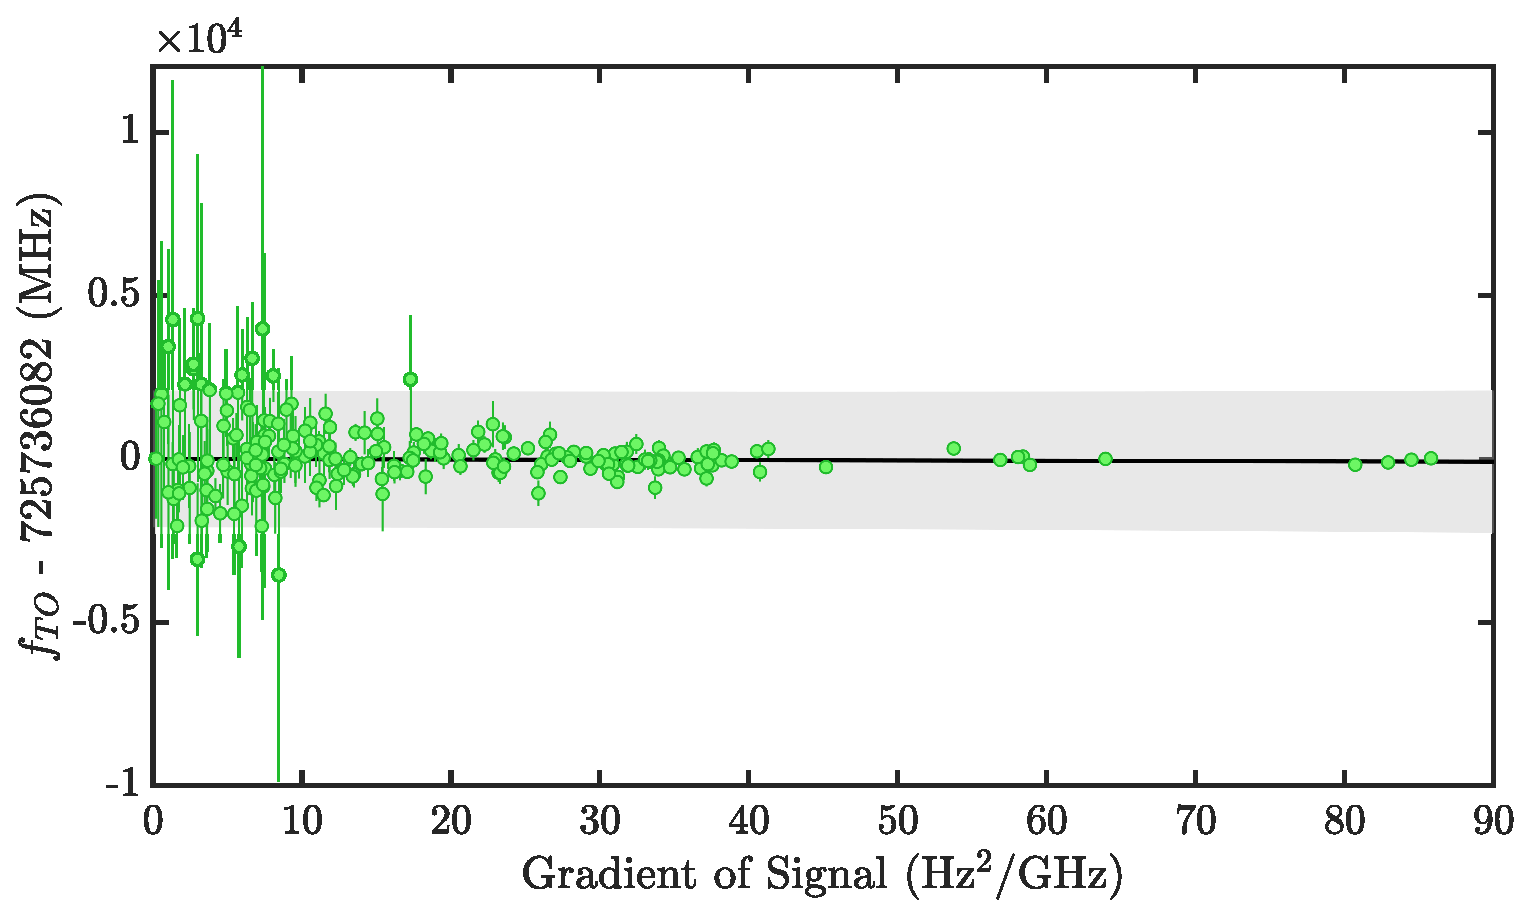
\includegraphics[width=\textwidth]{fig/tuneout/hyperpolz_graph_full}
		\caption{Measured tune-out dependence on probe beam intensity. The highest signal gradient (right) corresponds to a peak light field intensity of \(\sim4\times10^{8}\: \mathrm{W}\cdot \mathrm{m}^{-2}\). Error bars show the variance of binned data. The shaded region indicates the \(1\sigma\) observation interval, quantifying the variance in the data.  An uncertainty-weighted linear fit to the full data set data with parameters offset\(=725\,736\,082(3)\)~MHz and gradient -1(2) MHz/(Hz\(^2\)/GHz) is shown. 95\% confidence intervals in parameters are given in parentheses. This fit has $\chi^2$/dof=0.987 and determines that the gradient dependent tune-out shift is $30(50)$~MHz for the power used in the main measurement, which is statistically consistent with zero.
		    % former grad \(=-1.2(1.5)\)~MHz/(Hz\(^2\)/GHz)
		    }
	    \label{fig:hyperpolarizability}
	\end{figure}

    
\subsubsection{Theoretical treatment}

	The energy of an atom in the presence of an electric field \(E\) oscillating at a frequency \(f\) is 
	\begin{equation}
	\mathcal{E}=\mathcal{E}_0 - \frac{1}{2} \alpha(f) E^2 - \frac{1}{24} \gamma(f) E^4 + \ldots \, , \label{eqn:energy_shift}
	\end{equation}
	where \(\mathcal{E}_0\) is the energy of the unperturbed atom, \(\alpha(f)\) is the dynamic polarizability, and \(\gamma(f)\) is the (second) hyperpolarizability.  
	For a monochromatic light field, the time-averaged electric field amplitude is related to the intensity $I$ via
	\begin{equation}
	    E^2=\frac{2 I}{c \epsilon_0},
	\end{equation}
	where \(c\) is the speed of light and \(\epsilon_0\) is the permittivity of free space. 
	A tune-out measurement may be shifted due to the dynamic polarizability cancelling any contribution from the hyperpolarizability. 
	We can estimate this shift by noting that, by definition, \(\mathcal{E}=\mathcal{E}_0\) at the measured tune-out, and expanding the polarizability to first order about the tune-out.
	Thus Eq.~(\ref{eqn:energy_shift}) gives 
	
	\begin{equation}
	 (f-f_\mathrm{TO} ) = - \frac{1}{12} \gamma(f) \left(\frac{2 I}{c \epsilon_0}\right) \left(1\left/ \frac{\partial\alpha}{\partial f}\bigg|_{f=f_\mathrm{TO}} \right. \right).
	\end{equation}
	From the theoretical calculations, the dynamic hyperpolarizability  is $6.964\times10^{-58}$ $\mathrm{C}^4\mathrm{m}^4\mathrm{J}^{-3}$ (about $-1.12\times10^{7}$ a.u.) at the tune-out. The probe beam intensity in the experiment was less than $10^{9}\: \mathrm{W} \mathrm{m}^{-2}$ and thus a shift due to the hyperpolarizability is  constrained to be below 1.5~MHz, which is dominated by other systematic effects.

	% High precision atomic theory predicts that the dynamic hyperpolarizability at the tune-out is \(6.964\times10^{-58}\: \mathrm{C}^4\mathrm{m}^4\mathrm{J}^{-3}\), which is much larger than prior the prior prediction \(1.2\times10^{-58}\: \mathrm{C}^4\mathrm{m}^4\mathrm{J}^{-3}\) \cite{Grunefeld}/
	% Assuming the larger yields an estimate that the intensity-dependent shift is up to $2\times10^{-3}\: \mathrm{Hz} \mathrm{W}^{-1} \mathrm{m}^2$. 
	% Given the probe beam intensities used in this experiment were  $<10^{9}\: \mathrm{W} \mathrm{m}^{-2}$, the magnitude of this shift is $<1.5$~MHz and thus dominated by other systematic effects.
	% ($-2\times10^{6}$ atomic second hyperpolarizability units).

\subsubsection{Experimental treatment}

	We also constrained the effect of the hyperpolarizability using an independent experimental approach, by studying the effect of the light intensity on the the measured tune-out. 
	The gradient of \(\Omega_{\text{probe}}^2\) with respect to the laser frequency gives an indirect measurement of the intensity in the region of interaction, and the effect of beam power on the tune-out frequency (via this proxy) is shown in Fig.~\ref{fig:hyperpolarizability}.
	We evaluate the linear fit to the data at the experimentally-relevant gradient of $\approx 30$ Hz$^2$/GHz and find that the resulting shift is 30(50) MHz, which is statistically consistent with zero and with the (smaller) estimate made above on theoretical grounds.
	

\subsubsection{DC Electric Field}

	A worst-case estimate of any DC electric field background is $2~\text{kV}\cdot\text{m}^{-1}$. 
	We can use an approach similar to that of the hyperpolarizability  and find a worst-case shift of \(10^{-2}\)~MHz.

\subsection{Broadband Light}
	\label{sec:BBL}
	\begin{figure}
	    \centering
	    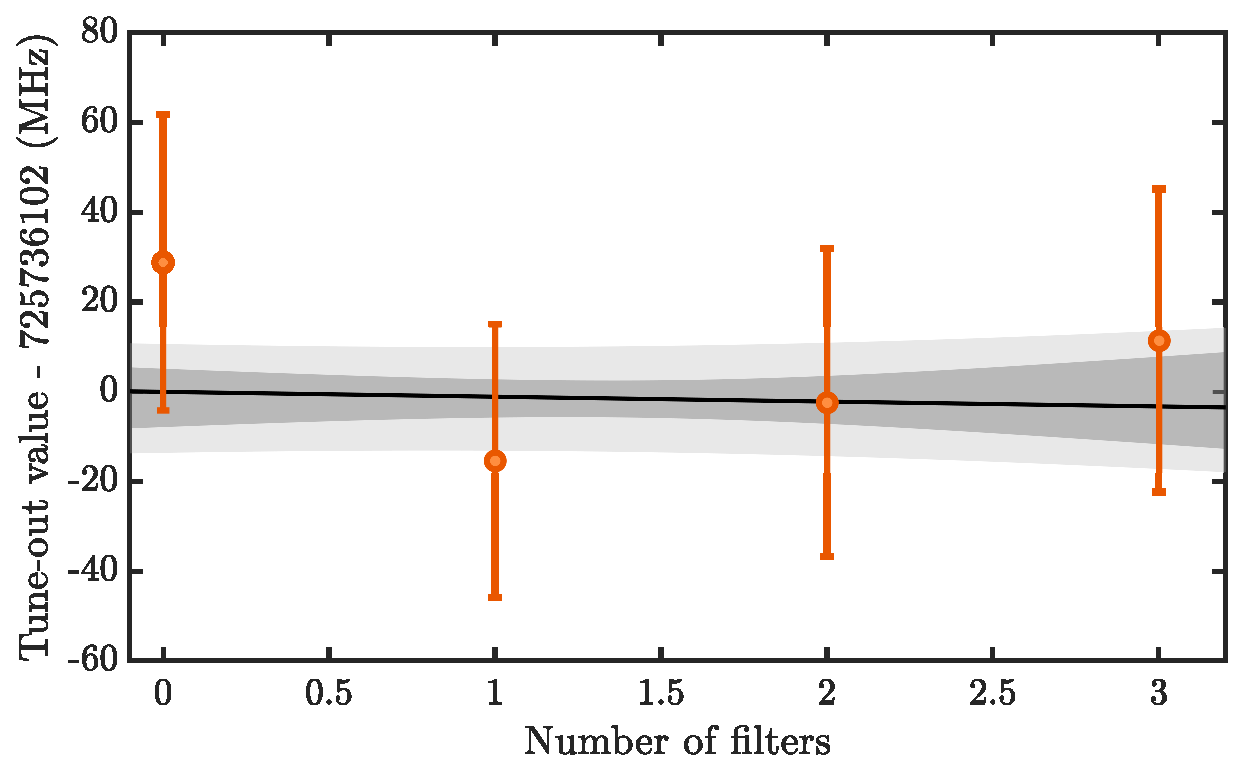
\includegraphics[width=\textwidth]{fig/tuneout/filt_dep_new}
	    \caption{The tune-out frequency as measured with fixed probe beam polarization and power, as a function of the number of filters in the beam path. The gradient of this dependence is -1(5)~MHz/filter, and hence zero within error. The linear fit has $\chi^2$/dof=0.6406. The light region shows the observation interval, and the dark region shows the confidence interval.
	    }
	    \label{fig:broadband light dependence}
	\end{figure}

	Broadband background light could be produced, for example, by  spontaneous emission in the Ti:S laser which is then amplified in the laser cavity. 
	In the presence of weak broadband light, the energy of the atom shifts by the (integrated) pointwise product of the spectral power density and the polarizability. 
	Because the magnitude of the polarizability increases superlinearly with the detuning from the tune-out ($|\alpha(f)| > \alpha'(f) (f-\fto)$ for large detunings), this effect puts a large weight on the tails of the laser line profile $g(f,\Gamma)$ and may shift the apparent tune-out from its actual value by contributing an energy proportional to $\int g(f,\Gamma)\alpha(f)~df$. 
	This places demanding constraints on the tolerable spectral background of the probe laser. 
	This has been a challenge for measurements in other species \cite{HolmgrenThesis}. 
	
	Our use of a frequency doubled laser system provides some protection from this because the doubling cavity suppresses broadband light that might originate in the Ti:S, unless it happens to have a wavelength equal to a multiple of the doubler's free spectral range. 
	Futher suppression is obtained by passing the probe beam through a series of optical filters: a 450~nm shortpass filter (Thorlabs FESH0450, optical density $>5$ between 450~nm and 1200~nm), a 415~nm band-pass filter (Semrock FF01-415/10-25, with a 27~THZ (15.3~nm) FWHM and optical density $>4$ between 250-399~nm and 431-1100~nm), and finally an angle-tunable filter with a 0.9~THz (0.5~nm) FWHM, which we centred on \(\sim 413\)~nm.

	In principle, one could use a spectrometer to measure the spectral power density of the background, but the requisite dynamic range to observe such small effects near a laser peak makes this unfeasible.
	Instead we used a scheme similar the one described in \cite{Leonard15}, and measure the tune-out as a function of the number of (progressively narrowing) filtering stages.
	We can then estimate the shift in the  final measurement. 
	As shown in Fig.~\ref{fig:broadband light dependence},  the measured tune-out frequency is independent of number of filters (within statistical error). 
	Therefore we take the standard deviation between the various filters (\(30\)~MHz)  as the uncertainty associated with the spectral background.
	 

	    % \caption{Measured tune-out frequency for a constant probe beam polarization as a function of the number of filters the probe beam light passes through. We find that the gradient of this dependence is \rev{-1(5) MHz/filter, with a fit $\chi^2$/dof=0.6406}, and hence zero within error.



	\begin{table}
	\centering
	% \begin{ruledtabular}
	\begin{tabular}{l|r|r}
	\hline\hline
	Term              & Value &  Uncertainty \\
	\hline
	Measured Value      & 725\,736\,810             & 40      \\
	Polarization        & & \\
	\, \, - Birefringence & -100                   & 200   \\
	\, \, - Beam Anisotropy & 0                   & 150   \\
	Method Linearity    & 24                   & 30       \\
	Hyperpolarizability           & -30                   & 50   \\
	Broadband Light     & 0                     & 30      \\
	DC Electric field   & 0                     & \(\ll 1\) \\
	Wave-meter          & 0                     & 4    \\
	\hline
	Total               &  725\,736\,700            &  260\\
	\hline\hline
	\end{tabular}
	% \end{ruledtabular}
	\caption{Contributions to measured tune-out frequency with associated systematic uncertainties (MHz). The measured value is found using only polarization data measured after the vacuum chamber. The polarization row gives the average of the tune-out frequencies calculated using polarization data pre and post vacuum chamber relative to the measured value (equivalent to assuming the shift from one window is half of the shift calculated using the measurements after both windows), and the uncertainty is equal to the difference between these values. Note that uncertainties are added in quadrature.}
	\label{tab:results}
	\end{table}
% \subsection{Magnetic Field Pointing}
	
% 	Although we do not need perfect knowledge of the magnetic field orientation to employ the preceding method, the field pointing could drift during the months-long data acquisition period, and thus presents a potential source of systematic error.
% 	To constrain this effect, we simulated the magnetic trap \cite{Dall07_laser} and field stabilization system \cite{Dedman07} used in these experiments \footnote{The source code is available at \cite{mag_trap_simulator}.}.
% 	Such a systematic shift can be divided into two contributions: the short-time variation in field pointing due to an atom's motion within the trap during the interrogation, and any long-term drift due to imperfections in the field control system.
% 	In the trap configurations used in this experiment, the magnetic field at the trap centre subtends a  $5.9 \degree $ angle relative to the long axis of the chamber, with which the probe beam is aligned, and a $0.019 \degree$ angle relative to the horizontal plane. 
% 	Our simulations show that the polar angle of the magnetic pointing varies as $0.019 + 0.88 s \degree$, relative to the $x$ axis, where $s$ is the displacement in m.

	A summary of the systematic shifts is shown in Tab. \ref{tab:results}. 
	The main limiting factor in the accuracy of our value for $\fto$ is  the polarization of the laser light. 


\section{Discussion}
\label{sec:TO_discussion}
	Figure~\ref{fig:contributions} shows a comparison of contributions to the theoretical value of the tune-out and the uncertainties in both the experimental and theoretical determinations.
	The combined theoretical and experimental uncertainties yield a  \(\sigma{\sim} 260\)~MHz precision which is much smaller than the contribution of QED effects (\({\sim} 30 \sigma\)), and thus our measurement validates these calculations.
	The retardation correction to the dipole interaction is slightly larger than the combined uncertainty (\({\sim} 2 \sigma\)), but the contribution of finite nuclear size effects (\(5\)~MHz) are not resolvable at this precision. 
	 
	This is the first measurement with sufficient precision to probe the retardation correction, which is significant as they are typically omitted from calculations of the frequency-dependent polarizability \cite{Drake19, Pachucki19}. 
	Overall, we find a \({\sim} 2.5 \sigma\) difference between experiment and theory, including an estimate of the uncertainty due to terms excluded from the theoretical calculation.  
	Notably, if we ignore the retardation correction (as proposed in Ref.~\cite{Pachucki19} and implemented in tune-out frequency calculations for the first time in this work), then the difference is only \({\sim} 0.5 \sigma\).  
	The retardation contribution could be subject to a more stringent test if the measurement precision could be improved by an order of magnitude (see section \ref{sec:TO_conc} for comments towards this).
	
	\begin{figure}[t]
	    \centering
	    \includegraphics[width=\textwidth]{fig/tuneout/contribution_bar_chart_v7.png}
	    \caption{Theoretical contributions to the tune-out value in comparison to uncertainties in the theoretical and experimental determinations of the \(\TO\) tune-out frequency.}
	    \label{fig:contributions}
	\end{figure}


	
	Using this method we can infer the peak value of the energy shift induced in the atoms by the probe beam. 
	Through Eq.~(\ref{eqn:omega_probe}), a measurement of the shift in trap frequency determines the curvature of peak of the Gaussian optical potential energy surface. 
	Along with knowledge of the beam spot size at the focus, the inferred curvature completely specifies the geometry of the optical potential. 
	We typically achieve an uncertainty in the tune-out of approximately 1.2~$\text{GHz}$ per $\sqrt{N_\text{shots}}$, where \(N_\text{shots}\) refer to the number of BEC's used (including calibration and probe beam measurements). 
	A single scan takes approximately 700~s (12~minutes) and consists of 26 trap frequency measurements (BEC productions). 
	As such, one full scan (26 trap frequency measurements) gives an uncertainty of $\sim 1.2\;\mathrm{GHz}/\sqrt{26}=235$~MHz\footnote{The number of measurements taken to find the tune-out for a given polarization varies from 50 to a few thousand for the data presented here.}.
	Thus, we can indirectly measure the absolute energy shift in the $\MetastableState$ state with a sensitivity of $1.7\cdot10^{-33}\mathrm{J}/\sqrt{\mathrm{sec}}$, where the time is the probe beam interrogation time. 
	In the case of the measurement with the lowest frequency uncertainty in $f_\textrm{TO}$, (30~MHz), the minimum potential energy peak we can thus discern is approximately $10^{-35}\mathrm{J}$ ($U/k_B=3$~pK).

\subsection{Improvements upon past measurements}

	The past measurement of this tune-out frequency \cite{Henson15} obtained a 4 GHz uncertainty in the determined value of $\fto = 725.7249$ THz (6ppm). This was comprised of a 1.5 GHz statistical uncertainty and a 3.5 GHz systematic uncertainty. 
	The 263~MHz total uncertainty presented here amounts to relative precision of 0.4ppm, a 15-fold improvement. 
	The 40~MHz statistical error in the new measurement is 40-fold smaller than that of previous measurement, due mainly to three factors mentioned below. This is significant progress, but the ultimate precision is limited by the systematic uncertainty of 260 MHz (which is improved roughly 14-fold over the prior measurement).	There are two main factors underpinning the improved systematic uncertainty.

	\begin{itemize}	
		\item \textbf{Purity of probe laser light:} In conventional spectroscopy, one is typically interested in the resonances (i.e. peaks) in some spectrum. In this setting, the finite linewidth of the system's response provides some insurance against the possibility that the probe beam could be polluted by spectral power at wavelengths other than the desired driving frequency. The nature of the tune-out measurement is the opposite: Because the polarizability increases with detuning from the tune-out, spectral impurities become more problematic the further detuned they are. This was the leading systematic effect in the previous work \cite{Henson15}. Recalling section \ref{sec:BBL}, this effect is constrained to the level of 30~MHz in the present work, nearly 120-fold better than the first measurement. The use of a frequency-doubling cavity was a significant factor here. The cavity modes act as narrow filters (limited by the finesse of the cavity), and the nonlinear gain medium results in a quadratic increase in the suppression of off-resonant light.
		\item \textbf{Characterisation of polarization effects:}  The atomic tune-out point depends strongly on the polarization of the electric field with respect to the atom's quantization axis (see e.g. section \ref{sec:polz_dep}, especially Eqn. \ref{eqn:fto_stokes_eqn}). Accordingly, this work paid careful attention to measuring this dependence in order to obtain a single measured  value ($\fto(-1,0)$). In contrast, the previous measurement used only linearly-polarized light, and the direction of polarization relative to the atomic quantization is not known. As can be seen from Fig. \ref{fig:pol_TO}, this amounts to some 5 GHz in systematic uncertainty. However, the previous analaysis did not account for the dependence on the polarization of the laser.  The 4 GHz total uncertainty that was included in the prior measurement (mainly due to the prior point) can be combined with this estimate to re-evaluate the the total systematic error of the prior work at the level of 9 GHz, which is comparable to the 11 GHz difference between the measurements. 
	\end{itemize}	

	Despite a more thorough examination of the latter point in this chapter, the polarization of light remains the leading source of uncertainty. The main contribution, as discussed in section \ref{sec:systematic_effects}, is that the polarization of the light \emph{at the atoms} is not directly measurable. The improvement in statistical precision is a result of three technical differences:

	\begin{itemize}
		\item \textbf{Laser power:} The present measurement applied a 150 mW probe beam at the point of vacuum entry, whereas the original measurement used a 3 mW laser diode (subject also to losses when passing through the focusing optics). 
		\item \textbf{Probe wavelength precision}: The High Finesse WS-8 wavemeter, obtained especially for this measurement, affords a locking of the probe beam with $\approx$175-fold greater accuracy. Moreover, the day-to-day drift of the wavemeter in the previous measurement was up to 350 MHz \cite{HensonHonsThesis}, larger than the drifts relevant to the present measurement by a similar factor. 
		\item \textbf{Optical dipole potential determination:} Previously, the optical potential was detected by modulating the net trapping potential with a probe beam and using a `lock-in' technique \cite{HensonHonsThesis} based on Fourier analysis of the outcoupling signal of a continuous atom laser. The idea is that the outcoupling efficiency would be modulated at the probe beam modulation frequency, and the phasor of the response would cross zero amplitude (with a phase flip) at the tune-out point. However, this signal exhibited a very high variance and thus the final linear fit to determine the tuneout was subject to significant statistical uncertainty. In contrast, the method employed in this work provides trap frequency measurement accurate to a few dozen ppm \cite{Henson22_PAL}, drastically improving the accuracy of $\fto$ as determined by the fitting procedures.
	\end{itemize}

	The effect of these factors can be seen in the following description of the sensitivity of the new method.
	The gradient of the linearized tune-out ecd dcdquation is
	\begin{equation}
		\frac{\partial \Omega_\textrm{net}^{2}}{\partial f} = \frac{4P}{\pi m c \epsilon w_0^4}\frac{\partial \textrm{Re}(\alpha(f))}{\partial f}
	\end{equation}
	Without loss of generality (within the assumption of linearity), we consider the problem of determining the detuning $\delta = f-\fto$ given a measurement of $\Omega_{net}$ at some laser frequency $f$.  Noting that the underlying trap frequency $\Omega_\textrm{trap}$ is known to within some parts in $10^5$, let us assume the uncertainty $\Delta$ in $\Omega_\textrm{net}$ is $\Delta_{\Omega_{net}^2}\approx\Delta_{\Omega_{probe}^2}$. We can then write
	\begin{equation}
		\Delta_{\delta} = \frac{\pi m c \epsilon w_0^4}{4P\alpha'}\Delta_{\Omega_{\textrm{probe}}^{2}},
	\end{equation}
	where $\alpha'$ is shorthand for the gradient with respect to frequency. It is evident that increasing laser power has a favourable effect on the precision. The improved wavelength precision reduces the systematic error in the means of generating the perturbing potential, and the improved trap frequency measurement reduces the systematic uncertainty in the actual response of the system, which both lead to improvements in $\Delta_{\Omega_{\textrm{probe}}^{2}}$


\subsection{Comparison With Previous Oscillator Strength Ratio Measurements}
	
	We can extend the approach taken in Ref. \cite{Mitroy13} to a three-level atom (c.f. section \ref{sec:TO_points}) and write the polarizability of an atom in the state $\ket{1}$ as 
	\begin{equation}
	\alpha_1(f) = \frac{\mathcal{F}_{12}}{E_{21}^2-h^2 f^2}+\frac{\mathcal{F}_{13}}{E_{31}^2-h^2 f^2}
	\end{equation}
	where $\mathcal{F}_{12}$ and $\mathcal{F}_{13}$ are the oscillator strengths, $E_{12}$ and $E_{13}$ are the excitation energies of the dominant transitions, $f$ is the photon frequency, and \(h\) is Planck's constant. The condition $\alpha(\fto)=0$ implies that
	\begin{equation}
		 \frac{\mathcal{F}_{12}}{E_{21}^2-h^2 \fto^2} = -\frac{\mathcal{F}_{13}}{E_{31}^2-h^2 \fto^2},
	\end{equation}
	and hence
	\begin{equation}
		\frac{\mathcal{F}_{13}^2}{f_{12}^2} = \left(\frac{E_{31}^2-h^2 \fto^2}{E_{21}^2-h^2 \fto^2}\right)^2.
	\end{equation}
	The fractional sensitivity of the ratio $X=\frac{\mathcal{F}_{13}^2}{\mathcal{F}_{12}^2}$ to the tune-out is
	\begin{align}
	    \frac{\delta X}{X} &= \frac{1}{X} \cdot  \frac{\partial X} {\partial f_{TO}} \delta f_{TO} \\
				    &=\frac{2  h^2 f_{TO} (E_{12}^2-E_{13}^2)}{(E_{12}^2-h^2 f_{TO}^2) (-E_{13}^2 + h^2 f_{TO}^2 )} \cdot \delta  f_{TO}\\
				    & = \frac{-2 f_{TO}^2 (f_1^2-f_2^2)}{(f_1^2-f_{TO}^2)(f_2^2-f_{TO}^2)} \frac{\delta  f_{TO}}{f_{TO}}
	\end{align}
	where $f_i=E_{1i}/h$.
	Given the dominant transition manifolds at 276.7465 THz (\(\MetastableState \to \TOUpperStateManifold \)) and 770.7298 THz (\(\MetastableState \to \TOLowerStateManifold\)), as well as our value for the tune-out frequency of \(f_{TO}=725.73670\) THz, we reach a fractional uncertainty in the oscillator strength ratio of 6~ppm.
	We can compare our measurement to others in the literature by using frequency of the dominant transitions and the measured tune-out value to estimate the sensitivity to the ratio of transition strengths. 
	We find that our measurement improves against the previous record of 15~ppm, reported in Ref.~\cite{Leonard15}. 
	We note that the relative uncertainty in $X$ equals the relative uncertainty in the ratio of transition matrix elements, which were the quantity calculated in Ref.~\cite{Leonard15}.
	We further note that this method is approximate and neglects the contribution from the DC polarizability, however this is a small effect and not needed for such coarse comparison of sensitivity. 
	Thus, we claim that our measurement of the $\TO$ tune-out wavelength produces the most precise constraint of relative transition rates in any atomic system to date. 


\subsection{Conclusion}
	\label{sec:TO_conc}
	Our experimental determination of 725\,736\,700\,$(40_{\mathrm{stat}},260_{\mathrm{syst}})$ MHz has a relative precision of $4\times 10^{-7}$, constituting the most precise measurement of atomic transition rate ratios to date \cite{Mitroy13}, and is 2.5$\sigma$ larger than the theoretical prediction. 
	This measurement determines the ratio of oscillator strengths to 6 ppm, which is a factor of two improvement on the previous record. 
	Furthermore, our novel method for measuring the dipole potential is able to discern a peak potential energy of as little as 10$^{-35}$ J. This is, to our knowledge, the highest precision in a potential energy measurement reported to date \cite{Henson22}.
	 
	In future precision measurements of tune-out points, significant improvements would follow from more precise calibration of the light polarization.
	One solution would be to use in-vacuum optics and systematically vary the angle of the beam axis relative to the magnetic field.
	These improvements would allow for independent tests of the scalar, vector, and tensor polarizabilities, thus yielding more information about the structure of the helium atom and QED itself.

	The method above could be used to measure other tune-out frequencies in helium or other species.
	It could also serve as a means to investigate other issues relating to QED. 
	If a future measurement could be made with MHz-level precision,  this tune-out could be used to calculate the nuclear charge radius of helium. 
	Thus this method, and its future improvements, may continue to  clarify the `jewel of physics.'

\vfill


\begin{flushright}
\singlespacing
{\emph{
``Imagination reaches out repeatedly trying to achieve some \\
higher level of understanding, until suddenly I find myself \\
momentarily alone before one new corner of nature’s \\
pattern of beauty and true majesty revealed. \\
That was my reward."}\\ 
- Richard P Feynman\footnote{Nobel banquet speech, 1965}}
\end{flushright}
\onehalfspacing




% \section{Note stash}



% \subsubsection*{Calculation of \(C\) and \(D\)}
% 	Consider light propagating along the \(z-\)axis (\textit{i.e.} light vector \(\vec{k} = \left(0,0,1\right)\)), the Jone's vector of this light is given by:
% 	\begin{align}
% 	    \vec{u} &= \begin{pmatrix}
% 	    u_{0,x} \\
% 	    u_{0,y} e^{i \phi_y} \\
% 	    0
% 	\end{pmatrix}.
% 	\end{align}
% 	By definition the stokes parameters are defined as follows (in order from first to fourth):
% 	\begin{align}
% 	    \mathcal{I} &= |u_x|^2 + |u_y|^2 \\ 
% 	    \mathcal{Q} &= |u_x|^2 - |u_y|^2 \\
% 	    \mathcal{U} &= 2 \text{Re} \left(u_x u_y^*\right) \\
% 	    \mathcal{V} &= -2 \text{Im}\left(u_x u_y^*\right)
% 	\end{align}
% 	where \(\vec{u} = (u_x,u_y,u_z)\). Note we only wish to consider that normalised Jones vector/ Stokes parameters, hence \(\mathcal{I}=1=u_{0,x}^2+u_{0,y}^2\). Let the plane formed by the light vector \(\vec{k}\) and the magnetic field vector at the atoms (the quantization axis) \(\vec{b}\) be the \(y-z\) plane, hence if the angle between the light vector and the magnetic field is \(\theta_k\) then:
% 	\begin{align}
% 	        \vec{b} &= \begin{pmatrix}
% 	    0 \\
% 	    \sin(\theta_k) \\
% 	    \cos(\theta_k)
% 	\end{pmatrix}.
% 	\end{align}
% 	Now if the polarisation is rotated by an angle \(\theta_\varepsilon\) the Jone's vector becomes 
% 	\begin{align}
% 	    \vec{u} &= \begin{pmatrix}
% 	    \cos(\theta_\varepsilon) u_{0,x} -\sin(\theta_\varepsilon) u_{0,y} e^{i \phi_y}\\
% 	    \sin(\theta_\varepsilon) u_{0,x} +\cos(\theta_\varepsilon) u_{0,y} e^{i \phi_y} \\
% 	    0
% 	\end{pmatrix}.
% 	\end{align}
% 	Now to align with equations \ref{eqn:C} and \ref{eqn:D} we want to rotate the axes such that the B-field is pointing along the \(z\)-axis, this corresponds to a rotation matrix of:
% 	\begin{align}
% 	    R_k &= \begin{pmatrix}
% 	 1& 0 & 0 \\
% 	 0 & \cos(\theta_k) & -\sin(\theta_k) \\
% 	 0 & \sin(\theta_k) & \cos(\theta_k)
% 	\end{pmatrix}.
% 	\end{align}
% 	applying this we get the Jone's vector in the B-field's frame of reference (denoted \(\vec{u}'= R_k \vec{u}\) as
% 	\begin{align}
% 	    \vec{u}' &= \begin{pmatrix}
% 	    \cos(\theta_\varepsilon) u_{0,x} -\sin(\theta_\varepsilon) u_{0,y} e^{i \phi_y}\\
% 	    \cos(\theta_k) \left[\sin(\theta_\varepsilon) u_{0,x} +\cos(\theta_\varepsilon) u_{0,y} e^{i \phi_y}\right] \\
% 	    \sin(\theta_k) \left[\sin(\theta_\varepsilon) u_{0,x} +\cos(\theta_\varepsilon) u_{0,y} e^{i \phi_y}\right] 
% 	\end{pmatrix}.\label{eqn:Jones_mag}
% 	\end{align}
% 	Note that in this notation equations \ref{eqn:C} and \ref{eqn:D} are
% 	\begin{align}
% 	    C &= 2 \text{Im}({u'_x}^* u'_y),\\
% 	    D &= 3|u'_z|^2 -1
% 	\end{align}
% 	as they have the B-field along the \(z\)-axis. Combining this with equation \ref{eqn:Jones_mag} we obtain
% 	\begin{align}
% 	    C&=2\cos(\theta_k)\text{Im}\left(\cos(\theta_\varepsilon)^2 u_{0,x} u_{0,y} e^{i \phi_y} -\sin(\theta_\varepsilon)^2 u_{0,x} u_{0,y} e^{-i \phi_y}\right)\\
% 	    &= 2\cos(\theta_k)\text{Im}\left(u_{0,x} u_{0,y} e^{i \phi_y}\right)\\
% 	    &= \cos(\theta_k)2\text{Im}\left(u_x^* u_y\right)\\
% 	    &= -cos(\theta_k) \mathcal{V}\\
% 	    D&=3\sin(\theta_k)^2 \left[\sin(\theta_\varepsilon)^2 u_{0,x}^2 +\cos(\theta_\varepsilon)^2 u_{0,y}^2 + 2\sin(\theta_\varepsilon)\cos(\theta_\varepsilon)u_{0,x}u_{0,y} \cos(\phi_y)\right] -1\\
% 	    \begin{split}&=\frac{3}{2}\sin(\theta_k)^2 \large[\sin(\theta_\varepsilon)^2 u_{0,x}^2 + (1-\cos(\theta_\varepsilon)^2) u_{0,x}^2 +\cos(\theta_\varepsilon)^2 u_{0,y}^2+\\&\quad\quad\quad(1-\sin(\theta_\varepsilon)^2) u_{0,y}^2 + 4\sin(\theta_\varepsilon)\cos(\theta_\varepsilon)u_{0,x}u_{0,y} \cos(\phi_y)\large]-1\end{split}\\
% 	    \begin{split}&= \frac{3}{2}\sin(\theta_k)^2 \large[-(\cos(\theta_\varepsilon)^2 u_{0,x}^2-2\sin(\theta_\varepsilon)\cos(\theta_\varepsilon)u_{0,x}u_{0,y} \cos(\phi_y)+ \sin(\theta_\varepsilon)^2 u_{0,y}^2) \\&\quad \quad + (\sin(\theta_\varepsilon)^2 u_{0,x}^2 + 2\sin(\theta_\varepsilon)\cos(\theta_\varepsilon)u_{0,x}u_{0,y} \cos(\phi_y) + \cos(\theta_\varepsilon)^2 u_{0,y}^2) + u_{0,x}^2 + u_{0,y}^2 \large]-1\end{split}\\
% 	    &=\frac{3}{2}\sin(\theta_k)^2 \left[-|u_x|^2 + |u_y|^2 + 1 \right] - 1\\
% 	    &=3 \sin^2\left( \theta_k \right) \left(\frac{1}{2} -  \frac{\mathcal{Q}}{2}\right) -1 
% 	\end{align}
% 	where we have used the fact that we are using the normalised Jones vector, hence \(u_{0,x}^2 + u_{0,y}^2 = 1\). 

% 	Consider the polarisation ellipse (the ellipse that the electric field traces out) see figure \ref{fig:ellipse}. Using the ellipse notation we can write
% 	\begin{align}
% 	    \mathcal{Q} &= \cos(2\psi) \cos(2\chi)\\
% 	    \mathcal{V} &= \sin(2\chi)
% 	\end{align}
% 	Next note that the power of a light field is proportional to its electric field amplitude squared so \(p_{min} \propto b^2\) and \(p_{max} \propto a^2\), where \(p_{min}\) and \(p_{max}\) are the minimum and maximum power transmitted through a linear polariser respectively. By trig laws we have 
% 	\begin{align}
% 	\cos(2\chi)&=\cos(\chi)^2-2\sin(\chi)^2\\
% 	&= \left(\frac{a}{\sqrt{a^2+b^2}}\right)^2 - \left(\frac{b}{\sqrt{a^2+b^2}}\right)^2 \\
% 	&= \frac{a^2-b^2}{a^2+b^2}\\
% 	\Rightarrow \mathcal{Q}&=\frac{p_{max}-p_{min}}{p_{max}+p_{min}} \cos(2\theta_\varepsilon)\\
% 	\sin(2\chi) &= 2\sin(\chi)\cos(\chi)\\
% 	&=2 \frac{a}{\sqrt{a^2+b^2}} \frac{b}{\sqrt{a^2+b^2}}\\
% 	&=\frac{2ab}{a^2+b^2}\\
% 	\Rightarrow |\mathcal{V}| &= \frac{2\sqrt{p_{min}p_{max}}}{p_{min}+p_{max}}
% 	\end{align}


	


 
 %Table here

% \subsubsection{Polarization in the Atomic Reference Frame}

% 	\subsubsection{Simplified Explanation}

% 	It can be helpful to consider this process for a simplified system with only linear polarization. In this case the measured tune-out will depend sinusoidally on the angle of the input polarization (\(\theta_{\mathcal{L}}\)). The above method is equivalent to using a sinusoidal fit in order to extract the maximum tune-out value in this dependence, corresponding to the \(f_{\mathrm{TO}}(-1,0)\). The choice of taking the maximum is equivalent to constraining \( \beta^T \). The above method is a natural extension of this simplified approach to also account for the circular component of the light field.


% Magnetic field

% Thermal Hyperpolarizability Shift

% Mean Field

% \hline
% \multicolumn{3}{c}{Theory}\\
% \hline
% Hyp. Polz           & $< 1.5$                   & 0.5     \\
% Magnetic field      & $< 2$                     & 0.01     \\
% DC Stark Shift      & $\ll 1$                   & 0.1    \\
% Thermal Hyperpolarizability Shift & $\ll 1$     & 0.1     \\
% Mean Field          & $\ll 1$                   & 0.1   \\






% 	To estimate the polarization we set up a Rochon prism after the beam exited the vacuum chamber through the LVIS hole and calculated the circularity of the light.




% \subsubsection{Alignment of probe beam}

% 	Alignment We employed three stages of successively increasing precision
% 	to align the probe beam with the magnetic trap, using a 2W? 532nm laser,
% 	followed by a 300mW 450nm beam, and finally using the tunable laser at
% 	approx 405nm?.
% 		The first beam was used for coarse alignment by scanning
% 	the vertical position of the focusing lens and dropping the BEC onto the
% 	phosphor detector.
% 		This technique has been used previously to align
% 	beams - reason being that the repulsive dipole potential of the 532nm
% 	beam creates a fissure in the BEC as the fallinc condensate diffracts
% 	around the beam.
% 		The effect is weak but visible as a dark stripe through
% 	the BEC - at least, ideally.
% 		Sadly, our ingenuity held us back (yet
% 	again).
% 		We used a pickoff plate - a large spherical optic which is
% 	weakly reflective at the target wavelength - for initial scans,
% 	deflecting a fraction of the beam onto a CCD (as described in the Laser
% 	System chapter).
% 		Unfortunately, Bryce dropped this optic at point point
% 	and the rim of the glass lost a chip.
% 		We did not notice for quite some
% 	time that this had altered the strain distribution on the transmitting
% 	surface of the optic, and actually completely destroyed the beam
% 	profile.
% 		How did we find this out, again? This led us to replace the
% 	optic with a mirror on a hinged mount, so we could remove the mirror and
% 	return it to a controllable position.
% 		Once we removed the damaged optic,
% 	we were quite quickly able to find a signal in the disturbed BEC.
% 		I
% 	think we eventually used the atom laser for a better visible signal -
% 	although the phosphor had a better dynamic range, the brightness
% 	difference was hard to see by eye, but integrating over several PALs
% 	gave us a density profile we could use.
% 		We aligned the beam with the
% 	fall path of the condensate by ensuring the destruction was in the
% 	centre of the falling condensate, and then raising the beam step by step
% 	until the signal vanished.
% 		At this point we figured we'd overshot the
% 	trap, so stepped back down and changed to another beam after marking
% 	beam position on the CCD.
% 		We then changed to the high power 450nm beam
% 	because it would produce a strong polarization response in the condensed
% 	atoms.
% 		We then ran successive trap frequency measurements while
% 	adjusting the beam position, looking for disturbances in the oscillation
% 	frequency under the same mechanism by which our measurement method
% 	works.
% 		When this signal reached a maximum with respect to position, we
% 	iterated adjustments in lens position along the beam axis with
% 	adjustments in pointing (as imperfectly aligned optics would couple
% 	these degrees of freedom).
% 		When this signal was maximized, we switched
% 	to the probe beam at 405nm.
% 		At this wavelength the atomic polarizability
% 	is positive so the beam is attractive.
% 		We therefore adjusted the
% 	sequence by switching off the beam at XXX ms after the trap release.
% 	When the beam was aligned we observed a second peak in the detection
% 	rate (picture), from the release of atoms trapped in the beam.
% 		We
% 	iterated this alignment procedure until the number of trapped atoms
% 	saturated - assuming this to be pointing at the BEC.
% 		Then we switched to
% 	alternating shots measuring the trap frequency, as in our measurement
% 	method, and adjusted the lens configuration until the frequency
% 	difference between the measurement and reference shots reached a
% 	maximum.
% 		Then, because the optical dispersion would be such that the
% 	beam pointing and focus would vary with wavelength, we repeated this
% 	procedure after taking steps of a few nm at a time towards the tuneout
% 	wavelength, eventually settling within a few MHz of the transition on
% 	the assumption that a few ppb change in frequency wouldn't bother us.
% 		We
% 	measured the distance from the focus lens to the chamber centre with
% 	reference to a technical diagram, and positioned the CCD at this
% 	distance away from the focus lens (including the reflection off the
% 	alignment mirror) but of course the beam before the focus lens would not
% 	have been perfectly collimated which might have affected the outcome.



	% The gradient of the line was found to vary, and in some cases invert in sign.
	% 	While initially puzzling, this turned out to be a useful validation of the trap frequency picture came from the inadvertent observation of a change of sign of the trap frequency change.
	% 	This was eventually ascribed to the sign change in the second derivative of a Gaussian function, which shows that the small-amplitude oscillation picture described above is actually quite accurate despite all the approximations (like, how big is the BEC?).
	% 	(PIC)
% % \hypertarget{quantum-depletion}{%
% \section{Quantum depletion}\label{quantum-depletion}}
\chapter{Quantum depletion of a harmonically trapped Bose gas}
\label{chap:QD}

\begin{adjustwidth}{3cm}{0cm}
\begin{flushright}
\emph{``Do not be content with the answer that is almost right; seek one that is exactly right...
	The Way is a precise Art.
	Do not walk to the truth, but dance."} - Eliezer Yudkowsky\footnote{\url{http://yudkowsky.net/rational/virtues/}}
\end{flushright}
\end{adjustwidth}


\section{Introduction} 
	One of Bogoliubov's seminal cotributions was to formalize the role of Bose-Einstein condensation in the physics of superfluidity \cite{Bogolubov47}.
	the mechanism underlying superfluid formation is the Bose-Einstein condensation of collective excitations.
	
	By transforming from the picture of a homogeneous system of interacting bosons to that of a free Bose gas of non-interacting quasiparticles, Bogoliubov showed that the macroscopically-occupied quasiparticle ground state corresponds to the superfluid part of the Landau two-fluid model.
	The population of excited quasiparticle modes then makes up the normal component of the fluid.
	
	This foundational theory is of broad relevance because the BEC and BCS regimes of superconductivity are characterized by superfluids of molecular dimers and of Cooper pairs, respectively.
	  

	In a bose gas, the collective excitations are constituted by oppositely-moving particles \cite{Vogels02}.
	
	Repulsive interactions between constituent particles lead to a zero-point population of quasiparticle modes, known as the quantum depletion, which persists even at zero temperature.
	
	The quantum depletion presents as an occupation of single particle modes with large momentum $p$ that decays like $p^{-4}$.
	In liquid helium, the depleted fraction is large (of order 90\% of the fluid) due to the strong interparticle interactions, but is generally very small in weakly-interacting dilute gases.
	Bogoliubov's theory makes accurate predictions of the total depleted population in ultracold atomic Bose-Einstein condensates (BECs) \cite{xu06,lopes17_depletion} and exciton-polariton condensates in solid substrates \cite{pieczarka20}.
	Therefore, detailed study of the quantum-depleted tails of the momentum distribution in ultracold gases is an attractive test for the Bogoliubov theory.

	This has been challenging to date because the tails are usually beneath the noise floor of optical imaging techniques, wherein the momentum spectrum is mapped onto the far-field density distibution following ballistic expansion.
	The use of Feshbach resonances to enhance the quantum depletion in strongly-interacting Bose gases has garnered recent attention \cite{Makotyn14,Fletcher17,Eigen18}.
	Measurements of the momentum distribution in these settings \cite{Makotyn14,Eigen18} found tails that deviate from the power-law behaviour, and a handful of theories have emerged \cite{Kira15_coherent,Colussi20,Smith14} in effort to understand this finding.
	
	While the particulars are still under debate, the general picture is that three-body interactions play important roles in the dynamical response of the gas to a switch to a large scattering length.
	In contrast, another meaurement in the a weakly interacting regime reported unexpectedly large momentum tails in the far-field density of a helium BEC released from a harmonic optical trap \cite{Chang16}.
	
	This is particularly surprising because conventional wisdom argues that the density decreases adiabatically during expansion, justifying treatment with a hydrodynamic approximation wherein the tails are predicted to vanish \cite{Qu16}.
	

	These observations are also in conflict with quantitative predictions of the tail shape drawn from the theory of contact interactions developed by Tan \cite{Tan08_energetics,Tan08_momentum,Tan08_virial}.
	The thermodynamic quantity called the \emph{contact} characterizes how s-wave contact interactions modify the short-range pair correlation function.
	
	The dual manifestation of this modification is that the contact determines the amplitude of the power-law decay of the momentum density in terms of the gas density and s-wave scattering length, which fully determine collisional dynamics in ultracold dilute gases.
	
	Two central properties of the contact, known as the adiabatic sweep theorem and generalized virial theorem \cite{Tan08_momentum,Tan08_virial}, have been verified via radio spectroscopy \cite{Baym07,Punk07,Braaten10} of degenerate Bose \cite{Wild12} and Fermi gases \cite{Stewart10,sagi12}.
	
	While the Bogoliubov prescription breaks down in strongly-correlated systems \cite{Lopes17_quasiparticle}, Tan’s theory applies for arbitrary spin mixtures at any density, temperature, and geometry, and so both theories are expected to agree in the weakly interacting regime.

	Thus, it is surprising that the prior work reported such strong tails as this apparently contravenes both the Tan and Bogoliubov theories in the weakly-interacting regime where both have otherwise been demonstrated to be accurate.
	One possible implication of this finding would be that some feature of harmonically trapped helium condensates violate the minimal assumptions of both theories, which would warrant further study.
	On the other hand, far-field measurements in general might not provide a straightforward means of examining the quantum depletion even in weakly interacting gases.
	As far-field measurements play a central role in study of ultracold gases, it is important to verify the anomaly and understand its origin in order to glean further insight.

	To this end, we revisit the measurement of the momentum distribution of a helium condensate expanding from a harmonic trap.
	
	We conducted experiments using a different apparatus, covering a range of densities twice as large as the prior work and using a magnetic trap in place of an optical dipole trap which ensures perfect spin-polarization of the condensate.
	
	We observe tails in the large-momentum part of the condensate wavefunction whose population is controllable in a manner consistent with the Tan and Bogoliubov theories.
	However, we show that not much can be said with certainty about the $p^{-4}$ decay due to inherent difficulties one faces when analysing power-law distributions in general.
	
	We describe, in detail, the limitations of inference of power-law parameters from empirical data with particlar emphasis on the relation between our findings and the results reported in \cite{Chang16}.
	
	Our measurements are complemented by simulations of the time-dependence of the momentum distribution using a stochastic Time-Adaptive Bogoliubov (STAB) method in the positive-P framework \cite{Deuar11,Kheruntsyan12}.
	
	These show that the non-adiabatic release of the trap is responsible for survival of the depletion, and that the depleted particles acquire additional kinetic energy from the mean-field energy of the condensate during the subsequent adiabatic expansion.
	
	These factors result in an amplification of the momentum tails relative to the in situ values, and are not captured in the hydrodynamic approximation.
	
	
	Finally, we discuss the concordance between our theoretical and experimental investigations in support of the visibility of the quantum depletion in the far-field and suggest productive means for future investigation.
	
\section{Background} 
	The Hamiltonian of a homogeneous system of interacting bosons can be written in terms of plane-wave field operators $\hat{a_\kvec}$, labeled by the wavevector $\kvec=\textbf{p}/\hbar$, as
	\begin{equation}
		\hat{H} = \sum_{\kvec} \frac{\hbar^2k^2}{2m}\hat{a}_{\kvec}^\dagger \hat{a}_\kvec + \frac{g n}{2}\sum_{\kvec,\kvec',{\bf l}}\hat{a}_{\kvec+{\bf l}}^\dagger\hat{a}_{\kvec'-{\bf l}}^\dagger \hat{a}_{\kvec'}\hat{a}_{\kvec},
	\end{equation}
	in terms of the particle density $n$ and the effective interaction strength $g=4\pi\hbar^2a^2/m$, where $a$ is the s-wave scattering length and $m$ is the atomic mass \cite{PitaevskiiStringari,PethickSmith}.
   
    This Hamiltonian can be diagonalized by the Bogoliubov transformation to a free Bose gas of collective excitations through the operator transformation $\hat{b}_{\kvec}^\dagger = u_k \hat{a}_\kvec^\dagger + v_k \hat{a}_{-\kvec}$ \cite{Bogolubov47,PethickSmith}, where the $u_k$ and $v_k$ coefficients are given by
	\begin{align}
		u_{k}^2 &= \frac{1}{2}\left(\frac{\hbar^2k^2/2m + gn}{\epsilon(k)} + 1\right)~\textrm{and}\\
		v_{k}^2 &= \frac{1}{2}\left(\frac{\hbar^2k^2/2m + gn}{\epsilon(k)} - 1\right),\\
	\end{align}
	and where the denominator is the quasiparticle dispersion
	\begin{equation}
		\epsilon(k) = \sqrt{\left(\frac{\hbar^2k^2}{2m}\right)^2 + gn\frac{ \hbar^2k^2}{m}}.
	\end{equation}
	In the non-interacting ($a\rightarrow0$) limit, $u_k=1$ and $v_k=0$, so the transformation reduces to the identity and the dispersion is that of free particles.
	
	In general, the single-particle momentum density can be found using the inverse transformation and is given by
	 \begin{align}
	 \rho(\kvec) &= \langle\hat{a}_\kvec^\dagger\hat{a}_\kvec\rangle\\
		 &=\left(u_{k}^{2}+v_{k}^{2}\right)\langle b_{\kvec}^{\dagger}b_{\kvec}\rangle + v_{k}^{2}.
		 \label{eqn:popstats}
	 \end{align}
	wherein the quasiparticle population statistics follow the canonical ensemble as $\langle \hat{b}^\dagger_\kvec\hat{b}_\kvec\rangle = (\exp(\epsilon(k))-1)^{-1}$ \cite{PitaevskiiStringari,Chang16}.
	At finite temperatures, quasiparticle modes are thermally populated and deplete the condensate.
	 Even at zero temperature, when the thermal fraction vanishes, the $v_k^2$ term in Eqn (\ref{eqn:popstats}) persists giving a zero-point population of the quasiparticle vacuum \cite{Decamp18,Chang16}, which decays as $\lim_{k\rightarrow\infty}\rho(\kvec)\propto k^{-4}$ \cite{PethickSmith,PitaevskiiStringari,Chang16}.

	In the case of a harmonically trapped gas, one can employ the local-density approximation (LDA) to compute the amplitude of the $k^{-4}$ tail by  integrating $v_k^2$ across a Thomas-Fermi distribution \cite{Chang16}.
	A simpler approach is afforded by Tan's original theorems.
	The two-body contact is defined by \cite{Tan08_momentum,Braaten11}
	\begin{equation}
		\mathcal{C} = \lim_{k\rightarrow\infty}k^4\rho(k),
		\label{eqn:MomentumDef}
	\end{equation}
	where the contact $\mathcal{C}$ is the volume average of the local \emph{contact intensity} $\hat{C} = 32 \pi^2 a^2 \hat{n}^2$ \cite{Werner12_boson}.
	The contact is also related to the total energy $E$ through the \emph{adiabatic sweep theorem} \cite{Tan08_energetics},
	\begin{equation}
		\mathcal{C} = \frac{8\pi m a^2}{\hbar^2}\frac{\partial E}{\partial a}.
	\end{equation}
	In the Thomas-Fermi approximation, the energy of $N_0$ condensed bosonic atoms is related to the chemical potential via
	\begin{equation}
		\frac{E}{N_0} = \frac{5}{7}\mu = \frac{5}{7} \frac{\hbar \bar{\omega}}{2} \left(\frac{15 N_0 a}{a_\textrm{HO}}\right)^{2/5},
		\label{mu}
	\end{equation}
	where $a_\textrm{HO} = \sqrt{\hbar/(m \bar{\omega})}$ is the harmonic oscillator length and $\bar{\omega}=\sqrt[\uproot{2}\scriptstyle 3]{\omega_x \omega_y \omega_z}$ is the geometric trapping frequency \cite{PitaevskiiStringari,PethickSmith}.
	The sweep theorem yields
	\begin{equation}
		\mathcal{C} = \frac{8\pi}{7} \left(15^{2}(a N_0)^{7} \left(\frac{m \bar{\omega}}{\hbar}\right)^{6}\right)^{1/5},
		\label{eqn:TotalHarmonicContact}
	\end{equation}
	which can be simplified as $\mathcal{C} = 64\pi^2a^2 N_0 n_0/7$ by dividing out the peak density of a harmonically trapped condensate,
	\begin{equation}
		n_0 = \frac{1}{8 \pi}\left( (15N_0)^2 \left(\frac{m \bar{\omega}}{\sqrt{a \hbar}}\right)	 ^{6}\right)^{1/5}.
		\label{eqn:n0}
	\end{equation}
	By substitution into Eqn.
	(\ref{eqn:MomentumDef}) one arrives at the expression
	\begin{equation}
		\lim_{k\rightarrow\infty}\rho(k) = \frac{64\pi^2a^2}{7} \frac{N_0n_0}{k^4}
		\label{eqn:pred_scaling}
	\end{equation}
	for the asympototic momentum distribution of a harmonically trapped gas spin-polarized bosonic atoms.
	

	
	

\section{Experiment} 
	Information about the momentum distribution of trapped gases is generally obtained by absorption-imaging measurements of the spatial distribution after some finite time of flight.
	In contrast, metastable helium affords single-particle detection in the far-field regime and thus gives direct access to microscopic momentum information.
	The metastable $\metastable$ state of helium, denoted He$^*$, is 19.8eV above the true ground state \cite{Hodgman09} which enables the use of a multichannel electron multiplier in combination with a delay-line detector (MCP-DLD) \cite{Manning10} for single-atom detection.
	Such setups have permitted the observation of many-body momentum correlations \cite{Hodgman11,Dall13} and the Hanbury Brown-Twiss effect in both condensed \cite{Schellekens05,Jeltes07,Manning10,Dall11} and quantum depleted atoms \cite{Cayla20}.
	
	
	Investigations of the quantum depletion in \mhe are challenging because the absence of a known Feshbach resonance precludes control over the contact $\mathcal{C}\propto((a N_0)^7\bar{\omega}^6)^{1/5}$ via the scattering length $a$.
	
	Given the small fixed $a=7.512$nm \cite{Moal06}, we test the validity of Eqn.
	(\ref{eqn:pred_scaling}) in the far-field by varying the density of the gas, $n\propto\left(N_{0}\bar{\omega}^3\right)^{2/5}$ (c.f.
	Eqn (\ref{eqn:pred_scaling}).
	
	We used two trap configurations with geometric frequencies $\bar{\omega} = 2\pi \cdot201$ rad Hz and $\bar{\omega} = 2\pi \cdot393$ rad Hz, and varied the endpoint of the evaporative cooling ramp to adjust the number of atoms in the condensate.
	
	
	Our experimental sequence, depicted schematically in Fig.
	\ref{fig:sequence}, began with BECs with between $2\times 10^5$ and $5\times 10^5$ $^4$He atoms polarized in the $\metastable(m_J=1)$ state and cooled to $\sim$ 300 nK by forced evaporative cooling in a harmonic magnetic trap generated by field coils in a Bi-planar Quadrupole Ioffe configuration \cite{Dall07}.
	
	After the trap is switched off, we transferred about one quarter of the atoms to the magnetically insensitive $m_J=0$ state with a radio-frequency (RF) Landau-Zener sweep to avoid distortion by stray magnetic fields.
	We deflected the $m_J=\pm 1$ clouds outside the detector field of view by implementing a Stern-Gerlach scheme immediately after the RF pulse.
	
	The centre of mass of the cloud then impacts on the detector after a $\tau = 417$ms time of flight following the trap switch-off.
	
	We interleaved the measurements just described with calibrations to determine the shot-to-shot variation in atom number, trapping frequencies, magnetic state transfer efficiency , and noise contributions.
	The technical aspects of these calibrations are discussed later in section \ref{sec:exp_details}.

	


	\begin{figure}[t]
	    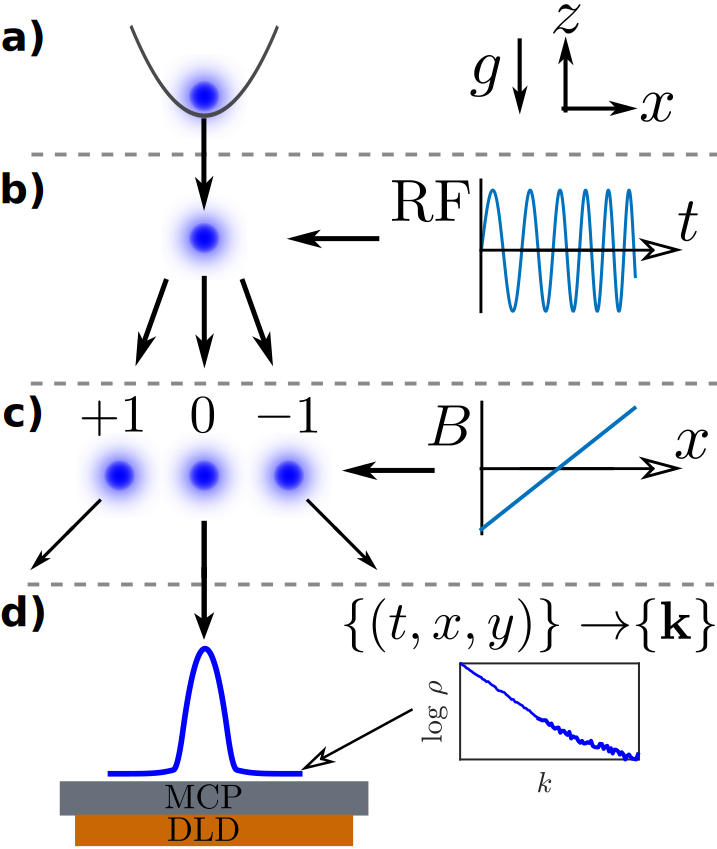
\includegraphics[width=0.4\textwidth]{fig/depletion/exp_cartoon}
	    \caption{Sketch of experimental sequence.
	A BEC is released from a harmonic trap with (a) and expands during freefall before being split into a superposition of the $m_J\in\{-1,0,1\}$ states (b) by an RF chirp.
	A magnetic field gradient separates the clouds (c) ensuring that only the magnetically insentitive $m_J=0$ cloud lands on the detector (d), from which the momentum information is reconstructed.
	The quantum depletion lies in the dilute tails at large momentum (inset, solid line).}
	    \label{fig:sequence}
	\end{figure}

	


\subsection{Analysis} 

	\begin{figure}[t]
	        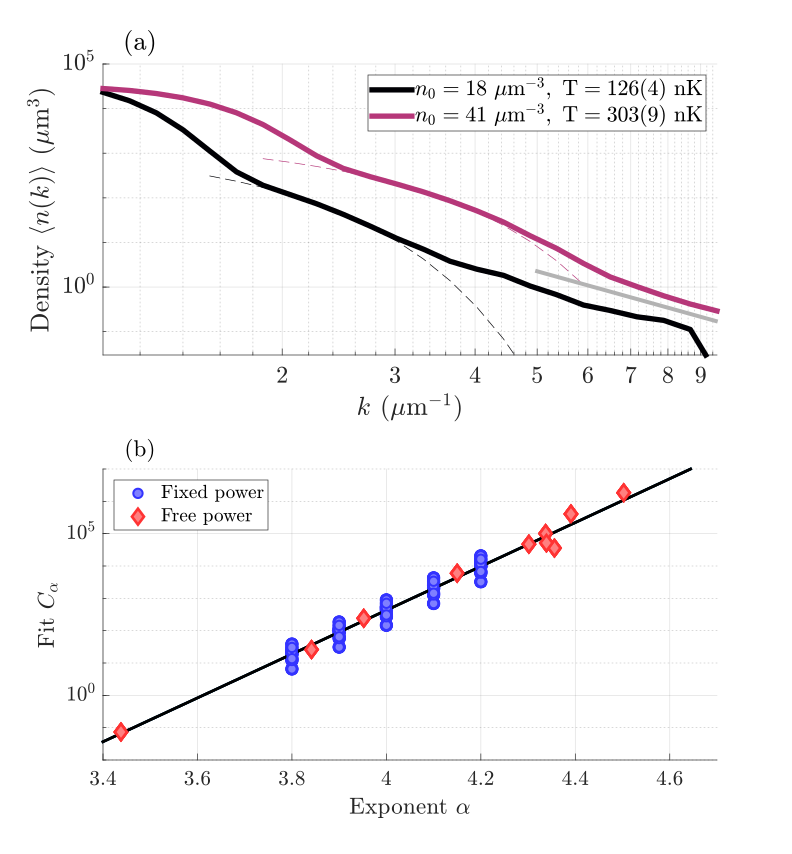
\includegraphics[width=0.5\textwidth]{fig/depletion/exp_density}
	        \caption{The empirical density of particle momenta for two traps (a), where the thermal parts (dashed lines) exponentially decay and give way to the depletion region, marked with grey dashed line proportional to $k^{-4}$.
	        In (b) we illustrate the large hidden systematic errors in a fit to the density which a power law.
	Leaving $\alpha$ as a free parameter gives a wide variation in best-fit exponents and scale coefficients.
	Blue squares show the amplitude coefficient $C_\alpha$ given a fixed exponent $\alpha$ fixed at five values within the range of fit results, applied to all data sets.
	The choice of $\alpha$ powerfully determines the coefficient $C_\alpha$, but the error bars (standard errors in fit parameters) are smaller than the markers in all cases.}
	        \label{fig:contact_determination_issues}
	\end{figure}


	In Fig.
	\ref{fig:contact_determination_issues} (a) we show the empirical density $n(k)$ for two data collection runs at the extreme values of $n_0$ we used.
	The three regimes of the condensate, thermal depletion, and quantum depletion span over five orders of magnitude in density.
	The thermal part of the distribution is well fitted by the momentum distribution of an ideal Bose gas,
	\begin{equation}
		n_T(k) =\frac{N_T}{\zeta(3)} ~\left(\frac{\lambda_{dB}}{2\pi}\right)^3 g_{3/2}\left(\exp\left(-\frac{k^2 \lambda_{dB}^2}{4\pi}\right)\right)
		\label{eqn:th_fun}
	\end{equation}
	wherein the thermal de Broglie wavelength $\lambda_{dB} = \sqrt{2\pi\hbar^2/(m k_B T)}$  yields an estimate of the temperature $T$ which ranges from 100 to 320 nK in our experiments.
	Here, $g_{3/2}(\cdot)$ is the standard Bose integral, $\zeta(\cdot)$ is the Riemann zeta function, and $N_T$ is the number of atoms in the thermal part.
	The thermal population decays exponentially with $k$, and hence cannot account for the counts we observe beyond $k\gtrsim 6~\micron^{-1}$.
	
	In rest of this section we present evidence in support of the identification of these counts with the quantum depletion.
	
	First, though, we show that the otherwise ubiquitous approach of a least-squares regression with a density function is inappropriate in this context.

\subsubsection{Issues with analysis of power laws}	
\label{sec:pow_issues}

	Proceeding with a routine fit of the $k$-space histogram with an additional term of the form $C/k^\alpha$ would appear to be an unobjectionable way to estimate the parameters of the purported quantum-depleted tail.
	However, fitting histograms with power laws is prone to return biased estimates of parameters and to drastically under-report uncertainties, especially when data is available over less than a couple of decades of dynamic range \cite{Clauset09,Virkar14}.
	
	As the authors of \cite{Clauset09} note, ``In practice, we can rarely, if ever, be certain that an observed quantity is drawn from a power-law distribution.
	The most we can say is that our observations are consistent with the hypothesis that $x$ is drawn from [a power law]"
	In this section, we demonstrate some of the problems with a least-squares regression using our data as a case study.
	In the next section we discuss our alternative approach and the inherent limitations of analysing data of this nature.
	
	If we augment the fit function (Eqn.
	(\ref{eqn:th_fun})) with power-law term and leave $\alpha$ as a free parameter, the average exponent of over all runs is 4.2(4).
	
	For comparison, the prior work \cite{Chang16} reported power-law tails with an exponent 4.2(2).
	At first glance, one could simply determine the amplitude of the tails by fixing the exponent to 4, and perhaps achieve better results by using a fit weighting proportional to $k^4$.
	 
	Indeed if we do so, we find an average $C_{\alpha=4}$ which is approximately 8(2) times greater than the coefficient of Eqn.
	(\ref{eqn:pred_scaling}), and in general agreement with ref.
	\cite{Chang16}.
	However, there are issues which undermine the reliability of this otherwise standard approach.

	First, in Fig.
	\ref{fig:contact_determination_issues} (b) we illustrate how the choice of scaling exponent $\alpha$ leads to an exponential change in the scale coefficient $C_\alpha$ that one obtains from fitting to a fixed dataset.
	The coefficient $C_\alpha$ varies over about three orders of magnitude \emph{either way} as one uses different exponents $\alpha$ which lie within the range of uncertainties reported here and in the prior work \cite{Chang16}.
	
	Furthermore, this problem is not reflected in the error estimates in the fitting routines: The error bars representing the uncertainty in fit amplitude are smaller than the markers used in Fig.
	\ref{fig:contact_determination_issues} (b).
	
	A linear fit shows that $d \log_{10} C/d\alpha \approx 6.8$, from which we can infer the exponent that would yield an amplitude in good agreement with Eqn.
	(\ref{eqn:pred_scaling}).
	
	This turns out to be approximately 3.9, which lies within one standard deviation from the mean exponent obtained from the regression we just described.
	
	Conversely, we can estimate that the best-fit exponents reported in the prior work would lead to scale coefficients a factor of about 23 greater than their conclusions, and the associated variance could be even larger.
	It is easy to see that a well-intentioned choice of $\alpha$, which is not statistically different from the best-fit estimates, can lead to  conclusion which either agrees perfectly or disagrees catastrophically with the predictions of Eqn.
	(\ref{eqn:pred_scaling}).
	In particular if one assumes that the data conforms to a power law with $\alpha=4$, one is forced to conclude that the Tan theory is wrong, but the inherent -- hidden -- uncertainty in this approach precludes the possibility of such a definitive statement.


	Second, a deceptively reassuring result can be found by multiplying the empirical density by $k^4$, observing a flat region, and adding a constant term in an appropriately scaled model of the thermal region (i.e.
	Eqn.
	(\ref{eqn:th_fun}) multiplied by $k^4$).
	
	In fact, this offers no recourse from the issues described above and is not a definitive test for the presence of a power law or a way t obtain its parameters.
	Suppose the density decays as some $C k^{-(\alpha+\epsilon)}$: then following the rescaling operation $k^\alpha n(k)$, one then has a density which would be expected to be have the form $C k^{-\epsilon}$.
	
	A variation in the (true) $\alpha$ within the systematic variation above leads difference of a factor of $O(2^{0.1})\approx1.07$ over the range $5\micron^{-1}\lesssim k\lesssim10\micron^{-1}$ range reported here and in \cite{Chang16}.
	This variation is dominated by the statistical fluctuations arising in the individual density profiles from random sampling, and is not distinguishable from the run-to-run variation in the power law.
	
	Despite this, fitting such a weighted distribution is similarly sensitive to the choice of weighting function
	For example, fixing the fit exponent at $\alpha=4$ and changing the \emph{weighting function} (not the form of the fit) in the fit from $k^4$ to $k^{4.1}$ returns a coefficient different by a factor of ten.
	This points to one of the primary challenges with power laws; the exponent are strongly entwined with the rate of occurrence of rare events, which by definition are subject to large statistical errors and thus subvert even the most meticulous investigations.

	In sum, these problems with fitting power laws are ubiquitous, and made more difficult by the small range of $k$ which are visible in the helium experiments.
	In general, estimating the exponent of a purported power law is difficult and requires data spanning several orders of magnitude in scale \cite{Goldstein04,Clauset09,Virkar14,Hanel17}, which are not present in either helium experiment.
	The preferred statistical tools for analysing power law distributions are maximum likelihood estimators, as discussed in lucid terms in Refs.
	\cite{Clauset09,Virkar14}.
	However, in these particle detection experiments the limited sampling region and presence of spurious detection events (described below) mean that such estimators are not appropriate.
	In the next section we describe an alternative approach which does not require -- and conversely cannot determine -- a precise value of the scaling exponent.
	We hope this discussion provides the theoretical and experimental community with an understanding of some problems with heavy-tailed distributions and points the way towards a sound analysis of such phenomena in future works.
	 % which neither assumes the data conforms to the theory under test nor requires precise determination of the exponent of the power law.
	
	
	\begin{figure}[t]
	\begin{center}
		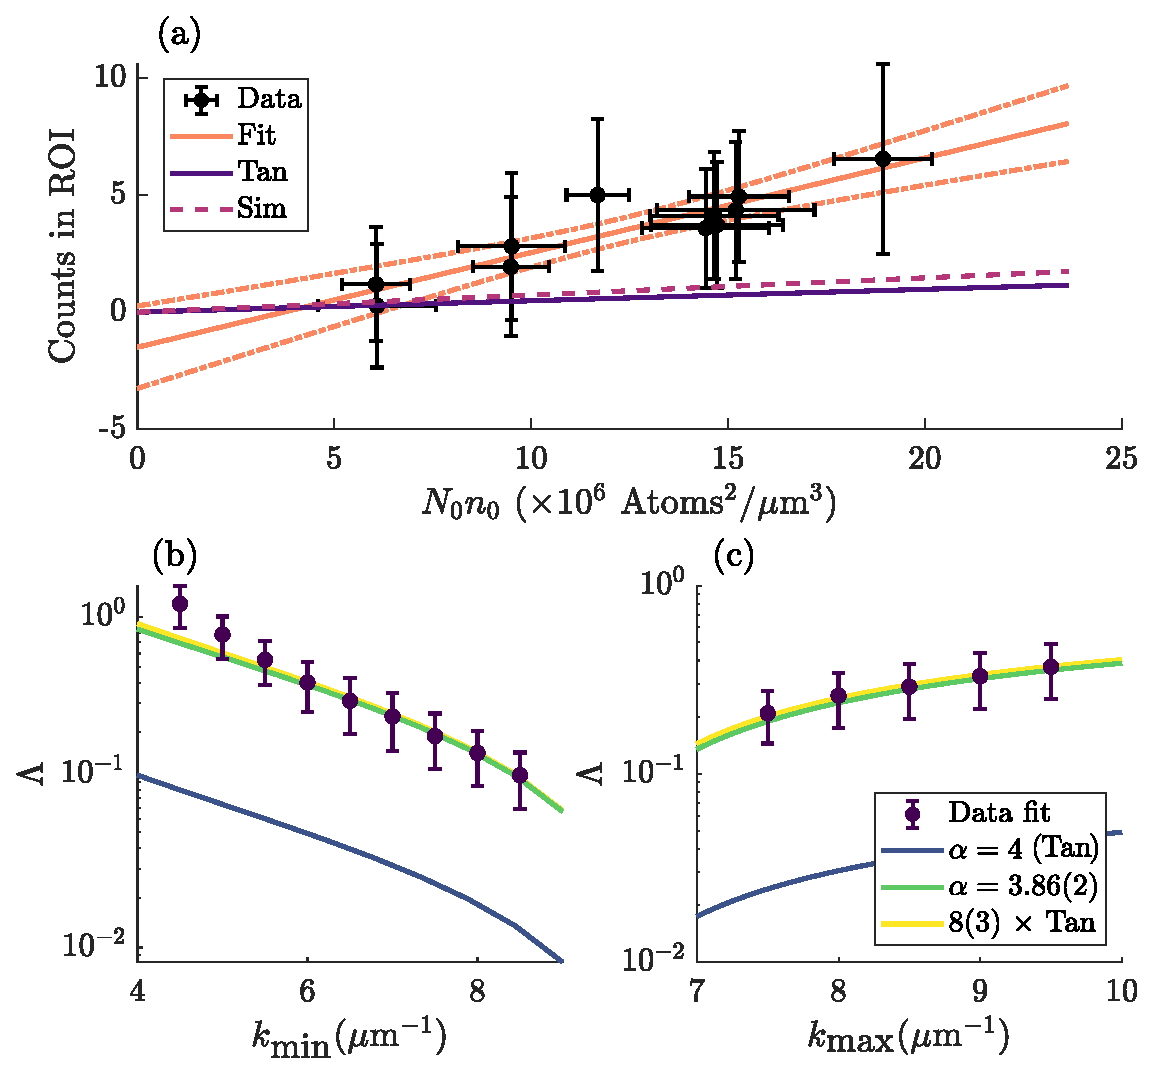
\includegraphics[width=\columnwidth]{fig/depletion/exp_results}
			\caption{A linear fit (a) shows that the product $N_0n_0$ is a good predictor of the number of counts within a region $(k_\textrm{min},k_\textrm{max})$, consistent with Eqn (\ref{eqn:pred_scaling}).
	The gradient $\Lambda_\textrm{fit}$ can be predicted using Eqn (\ref{eqn:pred_scaling}) but the two results disagree by a factor of about 8.
	The number of counts, hence $\Lambda$, depend on the choice of $k$ bounds, as shown in (b,c).
	This dependence does not provide estimates of $C$ or $\alpha$ because multiple hypotheses can produce indistinguishable behavior.
	In (b,c) we show predictions based on Eqn (\ref{eqn:pred_scaling}), along with the predictions of a density function $n(k)$ that is approximately 8(3) times Eqn.
	(\ref{eqn:pred_scaling}) and one that has exactly the amplitude $\mathcal{C}$ but a modified exponent.
	In (b), the deviation from the predictions at $k_\textrm{min}\lesssim6~\micron^{-1}$ is because the collection area starts to overlap with the thermal region.
			}

		\label{fig:exp_results}
	\end{center}
	\end{figure}

\subsubsection{Testing Tan's Tails}

	The prediction of the momentum tail shape (via Eqn.
	(\ref{eqn:pred_scaling})) captures a great deal of information, which can be split into two independently testable hypotheses.
	
	The first claim which we test is that the amplitude of this tail scales in proportion to the product $n_0 N_0$, and the second is the exponent of the density decay.
	Under the null hypothesis that the \emph{in situ} depletion survives the expansion and escapes the condensate undisturbed, one can integrate Eqn.
	(\ref{eqn:pred_scaling}) to predict the number of atoms whose wavevector has a modulus in the interval $k\in (k_\textrm{min}, k_\textrm{max})$, 

	\begin{equation}
		N_{k_\textrm{min},k_\textrm{max}} =\frac{\mathcal{C}}{2\pi^2}\left(\frac{1}{k_\textrm{min}}-\frac{1}{k_\textrm{max}}\right)
		\label{eqn:pred_num}
	\end{equation}
	Note that the integral of $n(k)$ is taken with the differential form $(2\pi^{-3})\d\kvec$ in spherical coordinates.
	For fixed $k_\textrm{min}$ and $k_\textrm{max}$, Eqn.
	(\ref{eqn:pred_num}) has the form $N_{k_\textrm{min},k_\textrm{max}} = \Lambda N_0n_0$ (c.f.
	Eqn.
	\ref{eqn:pred_scaling}).
	
	We can test this form directly by measuring the number of counts detected in the interval $(k_\textrm{min},k_\textrm{max})$ after producing a BEC of $N_0$ atoms with peak density $n_0$.
	
	The figure of merit for this description will be the goodness of fit of a simple linear regression.
	
	As above, we choose $k_\textrm{min}=6~\micron^{-1}$ which lies outside the thermal part for all our data sets.
	However, the $k$-space field of view is restricted by the detector radius to $k\lesssim5\times 10^6$ m$^{-1}$ in the $(x,y)$ plane, which is only just sufficient to reach past the edge of the thermal region.
	
	We thus face a tradeoff in the choice of $k_\textrm{max}$, therefore we define the bounds of our region of interest (ROI) by the minimum elevation angle $\phi_c=\pi/3$ rad and an upper bound of $k_\textrm{max} = 10\micron^{-1}$.
	This amounts to an ROI consisting of two vertically oriented conical sections, each with half-angle $\pi/6$, encompassing a total solid angle of $0.13\times 4\pi$ steradians.
	
	We must also account for the detector quantum efficiency of 0.08(2) and state-transfer efficiency of 25(2)\%, and combine all these factors into the total efficiency $\epsilon\approx0.23(5)\%$.
	After we discuss the results of this analysis, we will  examine the (lack of) effect of uncertainty in $\epsilon$ and the choice of $\phi_c$.
	% We find that the observed number $N_\textrm{exp}$ is 
	% Further, a straight line in a log-log plot is far from conclusive evidence of a power law as there exist other distributions (such as the log-normal and exponential distributions) which also present this way over larger domains than resolved in either of the helium experiments.	
	
	
	% Fixing the power at 3.86 yields 0.8(2) times the predicted contact
%     And at the 95% CI 
%         3.84 0.6(2) times Tan
%         3.88 1.1(3) times Tan
%     But it's not clear what this would mean, physically speaking...
%     so that would be approx 0.8(3) times Tan theor


	A linear fit of the form $\hat{N}_{k_\textrm{min},k_\textrm{max}} = \Lambda_\textrm{fit} n_0 N_0 + c$ yields a vertical intercept $c$ consistent with zero (c=-0.9,  95\% CI (-3.1, 1.2)) and a good correlation ($r^2\approx0.8$, $p=1\times10^{-3}$), providing evidence supporting the expected linear relationship.
	
	The correlation coefficient between the (normalized) variables $N_\textrm{exp}$ and $N_0n_0\propto(N_0^7\bar{\omega}^6)^{1/5}$ is 0.9.
	We conclude that the product $N_0n_0$ is a predictor of the depleted population, which is consistent with Eqn.
	\ref{eqn:pred_scaling}.
	We tested other combinations of the independent variables and found no physically-motivated combination provides a better fit.
	For comparison, a linear fit proves that the atom number itself is a poor predictor of the detected number ($r^2=0.05~,p=0.54$), as is the density alone ($r^2=0.4~,p=0.04$).

	The gradient $\Lambda_\textrm{fit}$ is of particular interest because it can be predicted using Eqn.
	\ref{eqn:pred_num}.
	Given an ROI, one can calculate $\Lambda_\textrm{pred} = 32 \epsilon a^2(k_{\textrm{min}}^{-1}-k_{\textrm{max}}^{-1})/7$.
	We find that the predicted slope disagrees with the empirical fit by a factor of $\Lambda_\textrm{fit}/\Lambda_\textrm{pred}= 8.3$, 95\% CI $(5.5,11)$.


	We are then tasked with reconciling the nonlinear scaling of the detected counts, which is consistent with the quantum depletion, and the disagreement over the absolute number of detected counts.
	We may look to understand the disagreement in terms of the deviation from Eqn.
	(\ref{eqn:pred_scaling}).
	We focus on the two most parsimonious alternatives: whether the tail amplitude is simply larger than expected (i.e.
	$n(k)=A\mathcal{C}/k^4$), or whether the tail decay is somehow modified (i.e.
	$n(k)=\mathcal{C}/k^{4+\delta})$.
	The former would imply that the derivation using the sweep theorem (or Bogoliubov theory in a local density approximation \cite{Chang16}) misses something essential about the system.
	The latter could point to some physical effect, either analogous to the prethermal dynamics of unitary gases \cite{Makotyn14,Eigen18,Colussi20,Kira15_coherent,Smith14} or another factor particular to the dilute regime.
	
	Ultimately, such a distinction between these hypotheses is not possible given the data at hand.
	
	% Specifically, through the appearance of the $k$ boundary values in Eqn.
	\ref{eqn:pred_num}, one could look to the $k$-depndence of $\Lambda_\textrm{pred}$ for a test of the density \emph{ansatze} above.
	Specifically, the density profiles $n(k)=A\mathcal{C}/k^4$ with $A=8(3)$ and $n(k)=\mathcal{C}/k^{\alpha}$ with $\alpha=3.86(2)$ both predict the variation of $\Lambda_{pred}$ with $k_\textrm{min}$ and $k_\textrm{max}$ with comparable accuracy (Fig.
	\ref{fig:exp_results} (b,c)).
	% In other words, if one insists on fitting a distribution of the form $k^{-4}$ then one concludes that the prediction for $\mathcal{C}$ is wrong by a factor of 8(3).
	It is thus not possible to tell whether we have a tail with the expected exponent but a greater weight, or the correct weight but a slower decay, or some combination of the two.
	% Indeed, the space of possible alternative hypotheses is practically infinite: One could find equally-apt distributions by modifying the power and coefficient together.
	Without the ability to precisely determine the exponent $\alpha$, there is insufficient evidence to conclude which of these is correct, therefore little can be said with certainty about which aspect of Eqn.
	(\ref{eqn:pred_scaling}) is incorrect or what physical effects might underpin this disagreement.
	Indeed, the predicted $k^{-4}$ behaviour is only a strict constraint inasmuch as it can be shown to persist (exactly) after the expansion, which as we argued above is not feasible, and argue below is not necessarily expected.
	One conclusion remains robust: There are about ten times as many detections in the depletion region as one would expect based on the Tan theory.
	
	Later in this section we provide technical details of our experiments and rule out several systematic factors which could lead to this disagreement.

	% Although our method provides a direct test of one aspect of Eqn.
	(\ref{eqn:pred_scaling}), it does not circumvent the fundamental challenges of analysing power laws.
	

	Nonetheless, the particular nonlinear scaling of detected counts with the predictor $N_0n_0$ is concordant with the tails' originating in the quantum depletion.
	Furthermore, our simulations indicate that the quantum depletion can survive the condensate expansion, presenting depleted tails in the far-field with modified amplitude.
	
	We are therefore faced with the conclusion that tails are indeed a signature of quantum depletion, albeit subject to some effect during expansion into which the present analysis can see no further.
	Given the similarity in settings and findings, the same could be said for the prior work \cite{Chang16}.
	% Comparing our work to \cite{Chang16}, given the similarity between experiments and consistency of the regression results above, our work can be said to corroborate their findings, albeit withthe prior work appears subject to the same limitations.
	
	
	% Our results could be seen as a count against the interpretation of these tails as a signature of the quantum depletion.
	
	% However, we note two pieces of evidence that give weight to this interpretation.
	
	% First, we are not aware of any other proposed physical effect which exhibits this specific nonlinear scaling relationship with respect to the atom number.
	% Second, we find evidence in our simulations (see below) that the momentum-space signature of the quantum depletion does survive the condensate expansion, and indeed appears in excess of the predicted \emph{in-situ} depletion.
	
	
	


\subsection{Experimental details}
\label{sec:exp_details}
\subsubsection{Trap configuration}

	We prepared our BECs with via forced evaporative cooling in a harmonic magnetic trap with trap frequencies $(45,425,425)$ Hz and a DC bias stabilized by our auxiliary field compensation coils \cite{Dall07,Dedman07}.
	For the tight trap we increased the coil current after the cooling sequence to obtain trapping frequencies $(71,902,895)$ Hz, ramping the field as a sigmoid step function to minimize in-trap oscillations.
	Note that the weak ($x$) axis of the trap is horizontal, with tight vertical confinement.
	The trap remained on for 150ms before switching the trap off with a $1/e$ time of $\approx38\mu$s.
	The condensates were allowed to expand for 2ms before we transferred some of the condensate into the magnetically insensitive $m_J=0$ state via Landau-Zener sweep to prevent distortion by stray magnetic fields.
	The RF pulse was created by a  function generator, amplified, and applied to the experiment chamber by a coiled antenna inserted into the BiQUIC coil housing.
	The pulse swept from 1.6-2.6MHz over 1ms and was centred on the fine structure resonance between the $m_J$ states.
	The determination of the transfer efficiencies $\eta_j$ for each of the $m_J = j$ states is discussed below.
	The sweep was $10^6$-fold wider than the Doppler broadening of the BEC which ensured uniform transfer at all momenta.
	Immediately after the RF sweep, the bias coils are switched off and auxiliary push coils in the vertical (Z) and weak horizontal (X) axes are activated using a fast MOSFET switch to implement a Stern-Gerlach separation of the $m_J = -1,~0,$ and $+1$ pulses.

	We use a Roentdek DLD80 multichannel plate and delay-line detector stack \cite{Manning10} located 859mm below the trap, which registers the arrival times and positions $(t_i,x_i,y_i)$ of each atom, indexed by $i$.
	
	The velocity of each atom relative to the centre of mass of each cloud is calculated by $(v_x,v_y,v_z) = t_{i}^{-1}(x_i-\bar{x},y_i-\bar{y},g_0(\tau^2-t_{i}^{2}))$, where $g_0$ is the local gravitational acceleration and the overbar denotes the within-shot average and $\tau$ ms is the time of flight of the centre of mass of the cloud.
	
	The far-field momentum is thus obtained via $m\textbf{v} = \hbar\kvec$.
	The velocity conversion assumes a point source but carries a negligible error of a few ppm as the in-trap BEC size is smaller than the detector resolution.
	
	The space and time resolution of the detector are 100 $\mu$m and 3 $\mu$s, respectively \cite{Henson18}, and the detector efficiency of $8(2)\%$ was determined from the collection efficiency of correlated atoms on the opposite sides of scattering halos \cite{shin19,shin20,Jaskula10}.
	

	\com{While the determination of the factor $\epsilon$ is important, the dominant uncertainty is the 25\% error in the detector efficiency.
	The collection area cutoff $\phi_c$ also factors in but this is precisely known.
	
	We performed the analysis described above for a range of $\phi_c$ and values of the QE and found that the excess of counts (expressed as $\Lambda_\textrm{fit}/\Lambda_\textrm{pred}$) was not significantly effected, which we summarize in Tab.
	\ref{tab:choice_indep}.}

	\begin{table}[b]
		\begin{tabular}{c c c c}
			\hline\hline
			% $k$ lim.
	($\micron^{-1}$) & fit $r^2$ &  $\Lambda_\textrm{fit}$ & $\Lambda_\textrm{fit}/\Lambda_\textrm{pred}$\\  
			% \hline
			% (6,7)  &  0.88     & 0.2(0.1,0.2) &   9.1(6.5,11.7)\\
			% (6,8)  &  0.85     & 0.3(0.2,0.3) &   8.4(5.7,11.1)\\
			% (6,9)  &  0.83     & 0.3(0.2,0.4) &   8.1(5.3,10.8)\\
			% (7,10)  &   0.79     & 0.2(0.2,0.3) &   7.8(4.8,10.8)\\
			% (8,10)  &   0.79     & 0.1(0.1,0.2) &   8.0(4.9,11.2)\\
			% \hline
			QE & fit $r^2$ &  $\Lambda_\textrm{fit}$ & $\Lambda_\textrm{fit}/\Lambda_\textrm{pred}$\\      
			\hline
			0.05    &   0.83   &   0.2(0.1,0.3)  &  6.8(4.5,9.1)\\
			0.06    &   0.83   &   0.3(0.2,0.4)  &  7.4(4.9,9.8)\\
			0.07    &   0.83   &   0.3(0.2,0.4)  &  7.8(5.2,10.5)\\
			0.08    &   0.83   &   0.4(0.3,0.5)  &  8.3(5.5,11)\\
			0.09    &   0.83   &   0.5(0.3,0.6)  &  8.7(5.8,11.6)\\
			0.1     &   0.83   &   0.6(0.4,0.7)  &  9.0(6.0,12.1)\\
			0.11    &   0.83   &   0.6(0.4,0.8)  &  9.4(6.2,12.5)\\
			\hline
			Half-angle & fit $r^2$ &  $\Lambda_\textrm{fit}$ & $\Lambda_\textrm{fit}/\Lambda_\textrm{pred}$\\
			\hline
			10$^\circ$    &   0.82   &   0.1(0.0,0.1) &  9.3(6.0,12.7)\\
			20$^\circ$    &   0.86   &   0.2(0.1,0.3) &  9.2(6.4,12)\\
			30$^\circ$    &   0.83   &   0.4(0.3,0.5) &  8.3(5.5,11)\\
			\hline\hline
		\end{tabular}
		\caption{The uncertainty in the detector quantum efficiency (QE) does not have a significant effect on the findings.
	Re-running the analysis using different QE yields fits that barely differ in the goodness of whose gradients do not significantly change.
	We also find that the choice of collection area has a weak effect, below statistical significance, on the result.
	Terms in brackets are the upper and lower 95\% confidence intervals.}
		\label{tab:choice_indep}
	\end{table}
	 % we show in Tab.
	\ref{tab:choice_indep}, this has no significant effect on the conclusion (namely, on the comparison $\Lambda_\textrm{fit}/\Lambda_\textrm{pred}$)
	% This could affect the outcome in two ways, first by changing the value of $\chi$ used in the prediction, and second through the factor of $N_{0}^7/5$ used to compute the condensate density $n_0$.
	



\subsubsection{Peak density calibration}

    The quantum depletion and contact are both predicted to depend solely on the condensed number and trapping frequencies via the condensate density, hence it is important to determine both quantities accurately.
	
    % In the Thomas-Fermi approximation, the peak density of the condensate can be written as $n_0 = \mu/g$, where $\mu$ is the chemical potential, $g=4\pi\hbar^2a_{1,1}/m$ is the effective interaction strength, $m\approx6.6\times10^{-27}$ kg is the atomic mass, and $a=7.512$ nm is the s-wave scattering length between pairs of atoms in the $m_J=1$ state \cite{Moal06}.
	
    The sole experimental parameters in the expression for the peak density (Eqn.
	\ref{eqn:n0}) are the geometric trap frequency $\bar{\omega} = \left(\omega_x\cdot\omega_y\cdot\omega_z\right)^{1/3}$, and $N_0$, the number of atoms in the condensate.
	
    We simultaneously determine the total atom number $N$ and trap frequency $\bar{\omega}$ in a single shot using a pulsed atom laser and use the thermal fraction (as below) to determine the condensed number $N_0$.
	

	The pulsed atom laser consists of a series of Fourier-broadened RF pulses centred on the minimum Zeeman splitting in the trap.
	
	The pulse transfers atoms in the trap to the untrapped $m_J=0$ state with an approximately constant transfer rate across the cloud.
	
	We outcouple approximately 2\% of the atoms per 100$\mu$s pulse for $\approx$200 pulses, which eventually depletes the entire trap.
	
	The atom laser thus prevents the detector from saturating and allows an accurate determination of the atom number, up to a factor of the quantum efficiency.
	
	We determine the trapping frequencies by inducing centre-of-mass oscillations with a magnetic impulse, and find the oscillation period from the atom laser pulses \cite{henson18ML}.


\subsubsection{Determining spin transfer efficiency}

	To calibrate the transfer efficiencies, we applied a weaker Stern-Gerlach than for the depletion measurement, resolving each $m_J$ cloud on the detector, as illustrated in Fig.
	\ref{fig:frac_cal}.
	

	\begin{figure}[!t]
	\begin{center}
		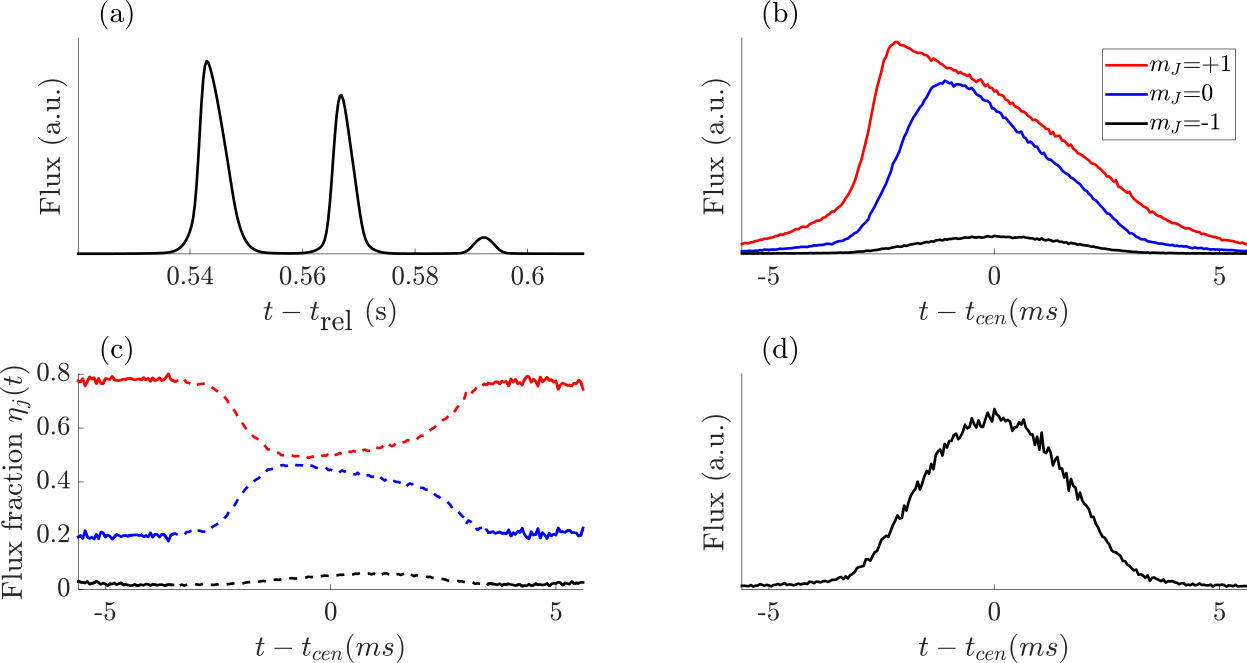
\includegraphics[width=\columnwidth]{fig/depletion/frac_cal_profile}
		\caption{Determining the RF transfer efficiency.
	The time-of-flight profiles of each pulse are resolved (a) by applying a weak Stern-Gerlach pulse during the time of flight.
	The pulses are aligned with respect their centre-of-mass (b) and used to determine the pointwise fraction ((c), dotted line).
	Detector saturation is evident in the peaks (dashed lines), but not in the thermal tails (solid lines), which are used to compute the transfer efficiency.
	Because of its lower flux, the $m_J=-1$ pulse does not show evidence of saturation (d) and is used to determine the thermal fraction.}
		\label{fig:frac_cal}
	\end{center}
	\end{figure}

	The efficiencies $\eta_J$ cannot be calculated by counting the atoms in each cloud because the detector saturates during the peak condensate flux, but we can compare the thermal parts.
	
	We align each cloud along the time (Z) axis and compute the pointwise fraction of the atomic flux $\phi(t)$ accounted for by each cloud, $\eta_j(t) = \phi_j(t)/\sum_j\phi_j(t)$, as depicted in Fig.
	\ref{fig:frac_cal}.
	
	The ratio of densities between the clouds is roughly constant in the thermal part, indicating the absence of important saturation effects and a spin transfer that is independent of $k$.
	
	The fraction of the original cloud transferred into each $m_J$ state is determined by taking the average $\langle\eta_j(t)\rangle$ over the thermal tails.
	
	We find these efficiencies are approximately 74\%, 24\%, and 2\% in all runs for the $m_J=+1$, 0, and -1 states, respectively.
	
	While the $m_J=0$ and $m_J=1$ clouds clearly saturate the detector, the small fraction ($\approx2\%$) of the atoms transferred to the $m_J=-1$ state does not (Fig.
	\ref{fig:frac_cal} (d)).
	
	A bimodal fit to the condensed and thermal parts, plus constant background, yields the thermal and condensed fractions.

	% \com{After a 2ms expansion the cloud is even more dilute than the trap, with a peak density that has approximately halved.
	Therefore the Because the contact in a mixed-species condensate \cite{Vassen16,Werner12_boson}, even if the condensate were still as dense as the in-trap distribution, the contact is reduced relative to the spin-polarized condensate.
	Considering also the reduced density after 2ms expansion, the production rate of quantum-depleted quasiparticles is expected to \emph{decrease} during this process, hence the observed effect is unlikely to emerge at this stage.}
	

% \subsection{Determination of thermal fraction}
	

% 	\begin{figure}[!h]
% 	\begin{center}
% 		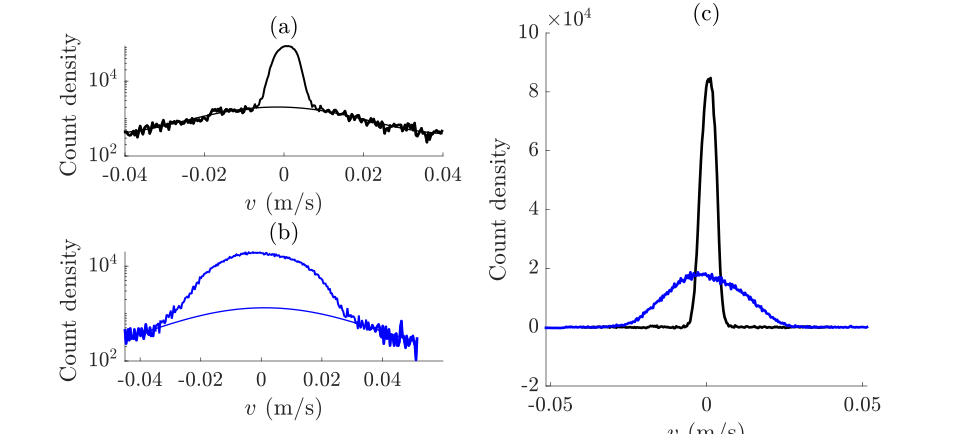
\includegraphics[width=0.8\textwidth]{fig/depletion/m1_frac_anal}
% 		\caption{Comparison of thermal fits in the unsaturated $m_J=-1$ pulse including 138 shots.
	The weak (X) and strong horizontal (Y) trapping axes are shown in (a) and (b), respectively.
	\org{would be helpful to label $v_x$ and $v_y$ to make it self-evident at 1st glance.} Both projections display a bimodal peak, with the condensate (dotted lines) and thermal parts (thick solid lines) easily distinguished.
	Fitting a Gaussian profile (thin solid line) to the velocity distribution of the thermal part yields the thermal number and temperature.
	Subtracting the fit leaves the condensate profile (c) which can be \blu{\dots something\dots} yields the condensed number.}
% 		\label{fig:thermal_frac}
% 	\end{center}
% 	\end{figure}


\subsubsection{Noise sources}
\label{sec:spinpop}

	In early tests of our measurement sequence we noticed a contamination of the signal by spurious counts.
	
	We inferred these were remnant counts from the $m_J=+1$ cloud as they were still visible when we ran an experimental sequence without the Landau-Zener transfer.
	
	This contamination appeared in a particular region of our detection image, and as such we were able to correct for it by subtracting their contribution from the counts collected during measurement shots.
	
	Generally, fewer atoms can be attributed to this noise than would be required to explain the discrepancy described in the main text.
	
	While the cause of the cross-contamination is unclear, we observe that the count density outside the region of interest is similar in both the shots with the RF pulse and those without.
	
	We hypothesize that the remnant counts are atoms transferred into the $m_J=0$ state by non-ideal behaviour of the Stern-Gerlach pulses.
	
	We note that only about one in a million atoms from the $m_J=1$ cloud present in this manner in a given shot.

	\com{Such counts constitute about 10(5)\% of the detection events in the ROI.
	Because it is not possible to distinguish \emph{which} atoms are spurious and which are genuine quantum-depleted particles, the preferred power-law analysis (the maximum-likelihood estimator) is not available.
	Basic MLEs are built assuming one has a sample drawn from a distribution of a single category; the probabilistic combination of two different sources of events falls outside the scope of this framework.}


% \begin{table}
% 		\begin{tabular}{ccccccc}
% 		\hline \hline 
% 		$n_0$ ($\mu$m$^{-3}$)  & $N_0\times10^{-5}$ & $\eta_\textrm{Th}$ & T (nK) & $N_\textrm{det}$ & $N_\textrm{pred}$ & $N_\textrm{det}/N_\textrm{pred}$ \\ 
% 		\hline 
% 		17(2) & 3.6(3) & 0.09 & 130(20) & 1.2(1) & 0.3(1) & 5(2) \\ 
% 		17(3) & 3.6(6) & 0.08 & 190(20) & 0.3(04) & 0.3(1) & 1(1) \\ 
% 		19(1) & 5.1(3) & 0.18 & 150(10) & 1.9(1) & 0.3(1) & 6(3) \\ 
% 		19(2) & 4.9(5) & 0.09 & 150(10) & 2.8(1) & 0.4(1) & 7(4) \\ 
% 		20(1) & 5.7(2) & 0.1  & 137(9)  & 5.0(1) & 0.5(1) & 10(4) \\ 
% 		39(4) & 3.8(3) & 0.11 & 252(3)  & 3.7(1) & 0.6(1) & 6(4) \\ 
% 		39(4) & 3.9(3) & 0.11 & 268(2)  & 4.4(1) & 0.6(1) & 8(5) \\ 
% 		39(3) & 3.8(3) & 0.1  & 249(3)  & 4.1(1) & 0.5(1) & 8(4) \\ 
% 		39(3) & 3.7(3) & 0.09 & 237(3)  & 3.6(1) & 0.5(1) & 7(4) \\ 
% 		39(3) & 4.0(2) & 0.14 & 312(3)  & 4.9(1) & 0.5(1) & 10(5) \\ 
% 		41(2) & 4.6(2) & 0.12 & 302(3)  & 6.6(2) & 0.7(2) & 10(6) \\ 
% 		\hline \hline 
% 		\end{tabular}
% 		\caption{Summary of results for each data run.
	The peak density is determined from measurements of the trapping frequencies and the condensed number (via $N_0=N_\textrm{tot}(1-\eta_\textrm{Th})$, using the total number $N_\textrm{tot}$ and thermal fraction $\eta_\textrm{Th}$).
	The number $N_\textrm{Detect}$ of atoms detected in the region of interest (results shown here for the largest ROI) can be compared to the predictions of the Tan theory, as in the main text.}
% 		\label{tab:run_results}
% 	\end{table}

	


	

% \subsubsection{Barriers to employing MLEs}

% 	The presence of these counts is one factor preventing a straightforward application of a maximum-likelihood estimator (MLE) to determine parameters of the power-law region.
	
% 	The basic principle of the MLE is to assume a functional form for the probability distribution $p(x|\theta)$ underlying the observed data $x$, and dependent on some parameters $\theta$.
% 	The zero of the derivative of the \emph{likelihood} function $L(\theta|x)$ with respect to the parameters $\theta$ then yields the most-probable parameter values given a set of observations $x$.
	
% 	In our context, one can assume a functional form for the probability distribution underlying atomic detection events (via a wavefunction ansatz).
	
% 	The detector dark counts can also be incorporated by assuming a uniform distribution, although this entails a cumbersome procedure to retain proper normalization.
% 	However, the dark counts present less than one detection per shot, on average, and thus might be ignorable without major consequence.
% 	The major obstacle to implementing an MLE is the finite detection region.
	
% 	Specifically, because the normalization condition 
	

%     \begin{figure}[!b]
% 	\begin{center}
% 		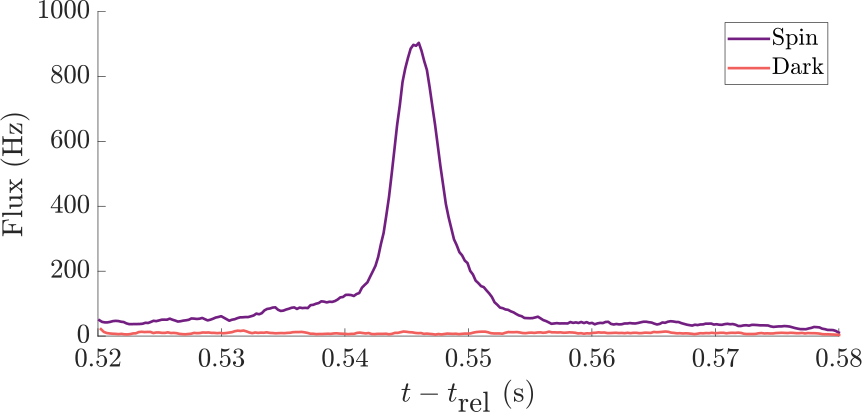
\includegraphics[width=\columnwidth]{fig/depletion/spinpop}
% 		\caption{Measured contribution of the detector dark counts and spurious spin counts to the time-of-flight profile.
% 	We accounted for the pulse at around 550ms and subtracted it from the measured profiles when computing the contact.
% 	After removing this background term, the density profiles above and below the condensate agree, indicating convergence on the true signal.
% 	For reference, the peak flux of the $m_J=0$ condensate is about a thousandfold greater than the peak shown here.}
% % 		\label{fig:spinpop}
% % 	\end{center}
% % 	\end{figure}

% % 	\begin{figure}[!h]
% % 	\begin{center}
% % 		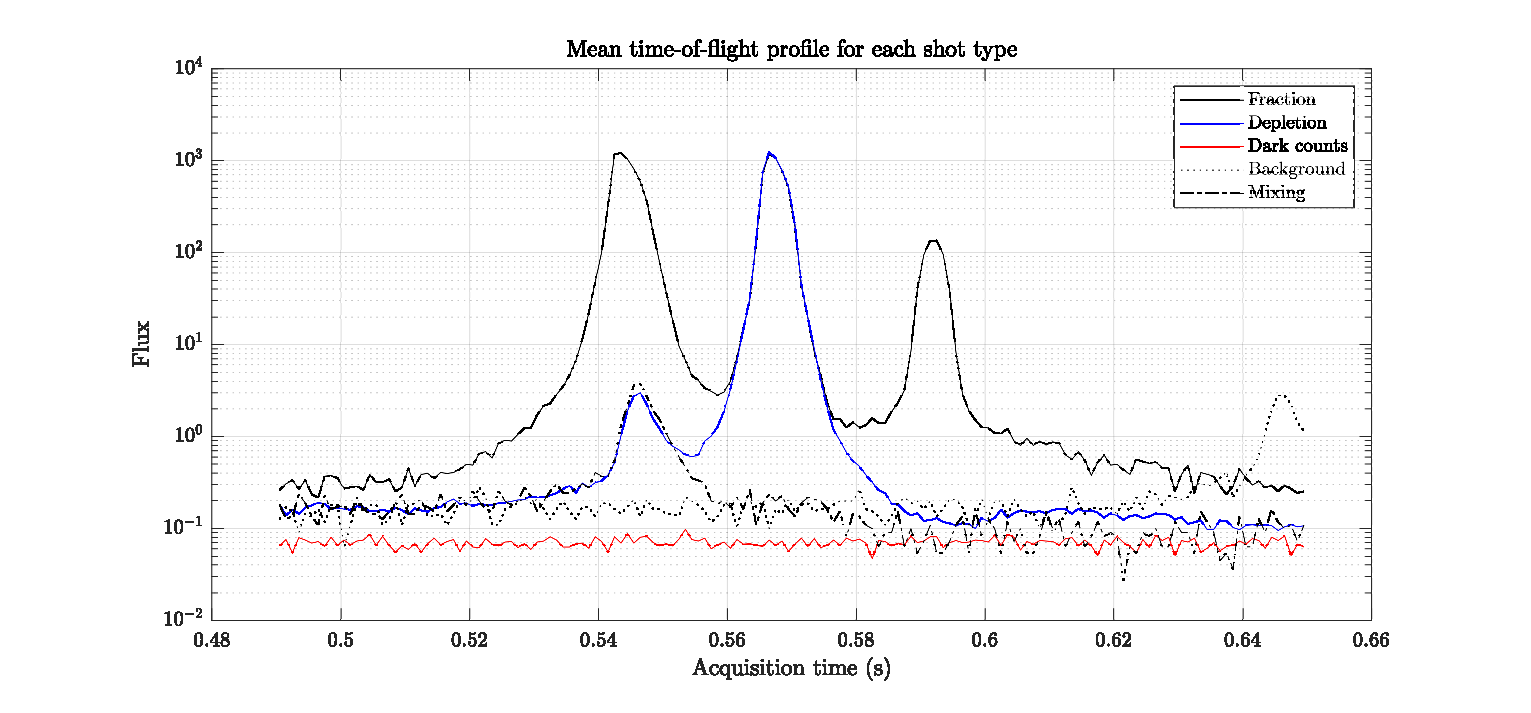
\includegraphics[width=\textwidth]{fig/depletion/profile_overlay}
% % 		\caption{Comparison of average time-of-flight profiles over a single data run for the quantum depletion measurement shots (blue, 871 shots), transfer efficiency calibration (black, 112 shots), detector dark counts (red, 871 shots), and spurious counts (dot-dash, 895 shots).
% 	The time window bounded by $|k|\leq 10\mu$m is indicated with dotted lines.
% 	Shaded area is the standard error over the entire run.}
% % 		\label{fig:tof_profile}
% % 	\end{center}
% % 	\end{figure}




% % Note that the temps disagree between axes, but within axes between clouds they are consistent(....ish).
% 	This means we can use the profile ratio method, which is also consistent with comparing the thermal number from the fits.
% % Perhaps comment on the thermal-subtracted part; the TF profile should have a sharp cutoff, but the smooth edges are suggestive evidence of this roll-off

% % \begin{figure}
% % 	\centering
% % 	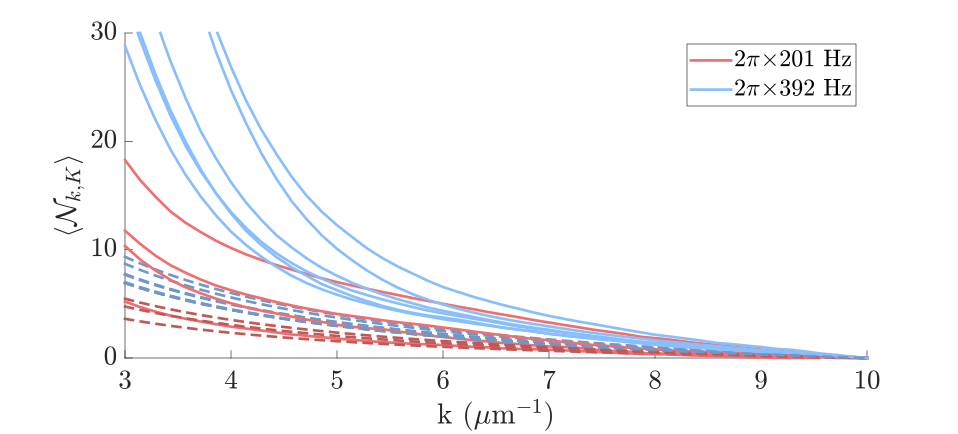
\includegraphics[width=0.5\textwidth]{fig/depletion/counts_per_run}
% % 	\caption{Number of counts detected in the region of interest in the depletion measurement (a), the spin mixing calibration (b), and the dark count calibration (c).
% 	An average of 3.0(5) counts were detected in the ROI in the spin-mixing calibration shot, and the background count rate was 0.4(2) counts per shot.
% 	Separate lines indicate separate \emph{runs}, i.e.
% 	sequences of shots with fixed parameters.}
% % 	\label{fig:num_counts}
% % \end{figure}








\section{Numerical simulations}
\label{STAB}
	\begin{figure}[b]
	        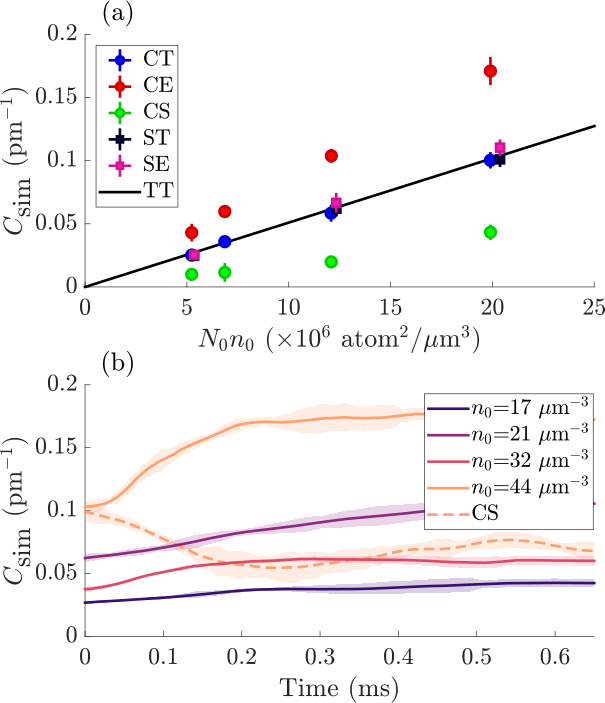
\includegraphics[width=\columnwidth]{fig/depletion/sim_results}
	        \caption{(a) Steady-state values of the simulated contact.
	Simulations of condensates released from a cigar-shaped trap (CT) are consistent with the Tan theory (TT) before release, and show an increase in contact after the trap release (CE).
	A slow relaxation of the transverse trapping frequencies (CS) shows a decrease in line with the predicted value of the lower density.
	Spherical traps (ST,SE) lack any directions of tight confinement, wherein a longer interaction time prevents the escape of depleted particles as seen in cigar traps.
	(b) the time-dependence of the contact stabilizes after a time on the order of $1/\omega_x$, several hundred $\mu$s.
	The difference between in-trap and expanded contact increases with the density of the condensate but is consistently about 1.7 times the Tan theory.
	For comparison, the experimental control pulses are implemented after 2ms of expansion.
	When the transverse trapping frequencies are reduced by half (dotted line), the in-situ contact relaxes.}
	        \label{fig:sim_fig}
	\end{figure}
	We performed simulations of the BEC expansion from harmonic traps using the first principles STAB method \cite{Deuar11,Kheruntsyan12}.
	
	The simulations included a cigar-shaped trap (marked CT in Fig.
	\ref{fig:sim_fig}) with parameters matched to the experimental conditions.
	
	The in-trap state was consistent with the adiabatic sweep theorem before release from the trap.
	
	Following expansion from the cigar trap (CE in Fig.
	\ref{fig:sim_fig})), the simulated tail amplitude increased and stabilized within a few hundred microseconds, much sooner than the 2ms delay between the trap release and application of the rf and Stern-Gerlach pulses.
	
	Fig.
	\ref{fig:sim_fig} shows time evolution of the tail amplitude for the simulated traps using the same ROI as the experimental setup.
	 
	In this configuration the steady-state value of the momentum tails was a factor of 1.64(9) above the predictions of Eqn.
	(\ref{eqn:pred_scaling}).
	

	To understand the disagreement with earlier theory \cite{Qu16}, which predicted no depletion survival, we also investigated the effect of adiabatic expansion on the in-trap depletion by simulating a slow decrease of the transverse trapping frequencies by a factor of two (CS), and found that the in-trap contact decreased roughly as predicted by Eqn.
	(\ref{eqn:pred_scaling}) in these instances --- see the dashed line in Fig.~\ref{fig:sim_fig}.
	
	We also found that the factor of disagreement (i.e.
	$C_\textrm{sim}/C_\textrm{Tan}$) between Eqn.
	(\ref{eqn:pred_num}) and the simulated tails depends on the angle choice of cutoff angle $\phi_c$.
	
	Put another way, the momentum distribution in the simulations is anisotropic and takes the form $f(\theta,\phi)/k^4$ - note that the average of an angle-dependent power law decay preserves the power-law behaviour.
	We find that $C_\textrm{sim}$ is larger for smaller collection regions that are more tightly concentrated about the vertical (strong) trapping axis, whereas larger collection angles (including areas closer to the weak axis) produce a lower $C_\textrm{sim}$.
	In particular, with cone half-angles of 10, 20, and 30 degrees, $C_\textrm{sim}$ was 2.2(3), 1.9(2), and 1.6(1) times $C_\textrm{Tan}$, respectively.
	We note that the experimental results (Tab.
	\ref{tab:choice_indep}) could be said to display a similar trend, but the result is not statisically significant.
	The implementation of the simulations is discussed in detail in the publication \cite{Ross21}.


\section{Discussion}
\label{sec:discussion}

	In sum, we find that the number of atoms in the large-$k$ tails is predicted by the product $N_0n_0\propto(N_{0}^7\bar{\omega}^6)^{1/5}$, in line with Tan's theory of the contact (Eqns.
	\ref{eqn:pred_scaling},\ref{eqn:pred_num}).
	
	However, the sensitivity of this relationship is significantly different than expected by a factor of order 8(3), which is not accounted for by any known systematic effects.
	The method we employ makes a clear distinction between what can and cannot be inferred about the form of the momentum tails, and indeed we find there is no decisive evidence in favour of tails that decay with $k^{-4}$.
	We do note that the prior work \cite{Chang16} reported results which fall within the uncertainty range of our analysis.
	Indeed, Fig.
	4 in \cite{Chang16} could be said to display the relevant scaling with respect to $N_0n_0$ but the reported values of the apparent contact should be considered along with the caveats discussed in Section \ref{sec:pow_issues}.
	
	Taken together with the simulations, our findings show that the survival of the quantum depletion into the far-field is plausible, but not as a straightforward mapping into the far-field density.
	In a non-interacting ballistic expansion, the far-field density distribution would be a direct realization of the in-trap momentum distribution of the cloud.
	
	However, this correspondence is known not to faithful because the dispersal of the mean-field energy into kinetic energy, known as the release energy, imparts some acceleration to the atoms during early expansion.
	
	This effect is responsible for the famous inversion of the cloud aspect ratio upon release from harmonic traps.
	

	As such we interpret our results as an indication that the depleted atoms are accelerated by the non-uniform mean-field energy of the condensate during the expansion.
	In detail, after a quench into the free particle regime, the condensate expands hydrodynamically on timescales of $1/\omega$.
	
	This is an adiabatic process for the low momentum depletion, whereby some depleted atoms are absorbed back into the condensate in agreement with \cite{Qu16}.
	However, the characteristic time for reabsorption is $\hbar/gn_0$, slow enough that quasiparticles in the particle branch of the Bogoliubov dispersion have sufficient velocity to escape the expanding cloud without being reabsorbed and thus transition to free atoms.
	
	This effect leads to the persistence of populated high-$k$ modes in the far-field, which were detected in the experiment.

	Moreover, an atom inside the BEC experiences an effective force from the gradient of the mean-field potential $\textbf{F} = -4\pi\hbar^2 m^{-1}a \nabla  n(x)$.
	
	This endows escaping depleted particles with a greater momentum, increasing the weight of the tails in the far-field.
	
	This effect is exacerbated in light atoms like $^{4}$He, whereas it would be suppressed by a $\sim500$-fold in $^{87}$Rb experiments \cite{Makotyn14} because the acceleration scales with $1/m^2$.
	
	Further, it is much easier for depletion atoms to escape and be accelerated in the transverse x-y directions from an elongated cloud because the distances $R_{TF}=\frac{1}{\omega}\sqrt{2gn_0/m}$ are reduced by $\bar{\omega}/\omega_{x,y}$, whereas the initial mean depletion velocities \textit{in situ} $v\sim \sqrt{2gn_0/m}$ are isotropic.
	Indeed, spherical clouds (SE) exhibit a much weaker effect than the elongated clouds (CE) owing to the longer escape time.
	This also presents as an increase in $C_\textrm{sim}$ for smaller collection regions.
	
	The statistical uncertainty in the experimental findings preclude a definitive comparison on this particular point.

	The interpretation just described is supported by another observation within the simulations:
	During the expansion we observe a decrease in the total number of depleted particles (reabsorption) and a simultaneous increase of the large-k population (forcing).
	
	This constitutes a partial explanation of the experimenal findings too, and results in tail amplitudes which are consistent with the quantum depletion multiplied by a constant factor.
	
	However, a mystery remains: Why is there an excess of particles in the depletion region which is so much greater than accounted for by this picture? 
	This issue should be resolved if far-field observations are to be interpreted in terms of the in-trap physics of interest.
	
	
	As we discussed, our systematic uncertainties are unable to account for the observed excess population of the quantum-depleted tails.
	Futher, despite the ultracold clouds being realized at finite temperatures, the thermal population of quasiparticles cannot account for the observed counts.
	
	The thermal quasiparticles in the Bogoliubov picture simply reflect a change of basis which maps identically onto the thermal population of constituent particles \footnote{See, for example, \cite{PethickSmith} Chap.
	8.3.}.
	
	Quasiparticles whose wavenumber exceeds that of the speed of sound lie within the particle-like branch of the bogoliubov spectrum, which for our considerations is on the order of $k\gtrsim2~\micron^{-1}$, well within the thermal velocities.
	
	Hence, given the exponential decay of thermally populated states, the large-$k$ tails are unambiguously \emph{not} thermal effects.
	

	In conclusion, our work expands the growing suite of far-field investigations of quantum depletion \cite{Cayla20,Chang16} and confirms that quantum depletion can, remarkably, survive past the lifetime of its original condensate.
	
	Our simulations clarify how the depletion can be visible in the far-field momentum distribution here and in earlier experiments, and that the hydrodynamic approximation does not capture sufficient short-wavelength information to make detailed predictions about the high-momentum behaviour.
	
	We thus find a partial explanation for the deviation of the far-field distribution from both the predicted in-situ depletion and the hydrodynamic reabsorption: The interplay between coherent absorption of Bogoliubov excitations and the dispersal of the chemical potential into kinetic energy, to which helium is particularly sensitive, result in a growth of the $k^{-4}$ tails of the momentum distribution during freefall.
	

	It would be informative to determine whether the outstanding discrepancy originates in the trapped condensate or is due to some unknown non-equilibrium effect during expansion.
	This question invites complementary studies of the \emph{in situ} depletion in \mhe BECs.
	
	Such an investigation requires an \emph{in situ} probe of the contact, such as RF spectroscopy or Bragg spectroscopy.
	The latter may be the most fruitful of the two simply because of the difficulty of interpreting the results from the former, which we sketch here.
	
	
	The basic principle of RF contact spectroscopy is to apply a monochromatic RF probe which is detuned from the resonance between two spin states, coupling atoms in the initial spin state to an untrapped channel.
	
	One then performs a differential measurement of the atom number and expects the signal strength to scale as $\omega_\textrm{RF}^{3/2}$ with the detuning from the RF resonance.
	The loss rate is also proportional to the difference of reciprocal scattering lengths $\Gamma\propto(1/a_\textrm{i,i}-1/a_\textrm{i,f})$ between pairs of atoms in initial-initial ($a_{i,i}$) and initial-final ($a_{i,f}$) spin states \cite{Braaten10,Wild12}.
	
	For He$^*$ (spin 1) the scattering lengths $a_{1,1}$ and $a_{1,0}$ are identical \cite{Leo01}, rendering the preferred $m_J=1-m_J=0$ transition unusable.
	
	On the other hand, $a_{1,-1} = 3/7 a_{1,1}$ \cite{Vassen16}, and the singlet transition can be driven without populating the $m_J=0$ state.
	
	In principle this could produce a detectable flux of atoms to perform sensitive in-trap contact measurements, however, collisions in the $^1\Sigma_{g}^{+}$ channel have large Penning ionization rates which lead to significant trap losses \cite{Leo01}.
	
	The ionization products would be detectable by in-vacuum channel electron multipliers but require theoretical work to disentangle from the spectroscopic signal.
	
	Further, while other atomic species offer Feshbach resonances by which to tune the inter-species scattering length (and hence signal or ionization rate), \mhe has no such feature.
	
	While such a measurement is not \emph{prima facie} impossible, Bragg spectroscopy may yield more readily interpretable results.



% \begin{abstract}

% Measurements of Tan's contact in expanding condensate conflict with predictions of the \emph{in situ} quantum depletion.
	% It is unclear how the depletion survives without a condensate, and even appears stronger in the far-field than before the trap release.
	% We confirm experimental observations of a slowly-decaying tails in the far-field, consistent with the survival of the quantum depletion.
	% Simulations of our experiment support shed light on the mechanisms behind the observations.
	% A gap between the numerical and empirical results remains an open question obstructing studies of quantum depletion in the far field.
% % max 600chars for PRL
% % \end{abstract}

% % \maketitle

% \section{Introduction} 
% 	The mechanism underlying superfluid formation is the Bose-Einstein condensation of collective excitations.
	
% 	This was formalized by Bogoliubov’s transformation \cite{Bogolubov47} of a homogeneous system of interacting bosons into a free Bose gas of collective excitations constituted by oppositely-moving particles \cite{Vogels02}.
	
% 	In a superfluid, the macroscopically-occupied quasiparticle ground state corresponds to the superfluid part, and population of excited quasiparticle modes constitute the normal component of the fluid.
	
% 	This foundational theory is of broad relevance because the BEC and BCS regimes of superconductivity are characterized by superfluids of molecular dimers and of Cooper pairs, respectively.
	  

% 	Interactions between constituent particles lead to a zero-point population of quasiparticle modes, known as the quantum depletion, which persists even at zero temperature.
	
% 	The quantum depletion presents as an occupation of single particle modes with large momentum $p$ that decays like $p^{-4}$.
% 	In liquid helium, the depleted fraction is large (of order 90\% of the fluid) due to the strong interparticle interactions, but is generally very small in weakly-interacting dilute gases.
% 	Bogoliubov's theory makes accurate predictions of the total depleted population in ultracold atomic Bose-Einstein condensates (BECs) \cite{xu06,lopes17_depletion} and exciton-polariton condensates in solid substrates \cite{pieczarka20}.
% 	Therefore, detailed study of the quantum-depleted tails of the momentum distribution in ultracold gases is an attractive test for the Bogoliubov theory.

% 	This has been challenging to date because the tails are usually beneath the noise floor of optical imaging techniques.
	
% 	A previous experiment \cite{makotyn14} sought to use a Feshbach resonance to produce a visible depleted fraction, but found that the momentum distribution saturated during expansion and did not display a power-law tail.
	
% 	% \com{This was because complex three-body effects play an important role in the pre-thermalization dynamics, and so the asymptotic momentum distribution is no longer characterized purely by two-body dynamics.
	% \cite{kira15_hyperbolic,kira15_coherent}}
% 	In contrast, another experiment found unexpectedly large momentum tails in the far-field of a weakly interacting helium BEC released from a harmonic optical trap \cite{chang16}.
	
% 	This is particularly surprising because conventional wisdom argues that the density decreases adiabatically during expansion, justifying treatment with a hydrodynamic approximation wherein the tails are predicted to vanish \cite{qu16}.
	

% 	These observations are also in conflict with anither successful and widely applicable theory of contact interactions developed by Tan \cite{tan08_energetics,tan08_momentum,tan08_virial}.
% 	The thermodynamic quantity called the \emph{contact} characterizes how s-wave contact interactions modify the short-range pair correlation function.
	
% 	A defining feature of the contact is that it determines the amplitude of the power-law decay of the momentum density in terms of the gas density and s-wave scattering length, which fully determine collisional dynamics in ultracold dilute gases.
	
% 	Two central properties of the contact, known as the adiabatic sweep theorem and generalized virial theorem \cite{tan08_momentum,tan08_virial}, have been verified via radio spectroscopy \cite{baym07,punk07,braaten10} of degenerate Bose \cite{wild12} and Fermi gases \cite{stewart10,sagi12}.
	
% 	While the Bogoliubov prescription breaks down in strongly-correlated systems \cite{lopes17_quasiparticle}, Tan’s theory applies for arbitrary spin mixtures at any density, temperature, and geometry, and both theories are consistent in the weakly interacting regime.

% 	Thus, it is surprising that the prior work observed such strong tails as this contravenes both the Tan and Bogoliubov theories in the weakly-interacting regime where both have otherwise been demonstrated to be accurate.
% 	This implies that either some feature of harmonically trapped helium condensates violate the minimal assumptions of both theories, or that far-field momentum measurements are not a straightforward means of examining the quantum depletion even in weakly interacting gases.
	
% 	It is important to verify and overcome this obstacle, as far-field measurements play a central role in study of ultracold gases.
	

% 	To this end, we revisit the measurement of the momentum distribution of a helium condensate expanding from a harmonic trap.
	
% 	We conducted experiments using a different apparatus and analysis, covering a range of densities twice as large as the prior work, and use a magnetic trap in place of an optical dipole trap which ensures perfect spin-polarization of the condensate.
	
% 	We observe tails in the large-momentum part of the condensate wavefunction which exhibit a $p^{-4}$-like scaling, and whose amplitude scales in proportion to the condensate population in a manner consistent with the Tan and Bogoliubov theories.
	% However, the absolute amplitude significantly exceeds the predictions of the in situ depletion by a constant factor, corroborating the prior work.
	

% 	Our measurements are complemented by simulations of the time-dependence of the momentum distribution using a stochastic Time-Adaptive Bogoliubov (STAB) method in the positive-P framework \cite{Deuar11,Kheruntsyan12}.
	
% 	These show that the non-adiabatic release of the trap is responsible for survival of the depletion, and that the depleted particles acquire additional kinetic energy from the mean-field energy of the condensate during the subsequent adiabatic expansion.
	
% 	These factors result in an amplification of the momentum tails relative to the in situ values, and are not captured in the hydrodynamic approximation.
	
% 	However, quantitative disagreement between our simulations and experimental data rule out the release energy as a complete explanation for the observed excess counts.
% 	We discuss some important qualitative factors which nonetheless support the identification of the high-momentum tails with the quantum depletion and suggest an informative complementary approach for future experiments.


% \section{Background} 
% 	The Hamiltonian of a homogeneous system of interacting bosons can be written in terms of plane-wave field operators $\hat{a_\kvec}$, labeled by the wavevector $\kvec=\textbf{p}/\hbar$, as
% 	\begin{equation}
% 		\hat{H} = \sum_{\kvec} \frac{\hbar^2k^2}{2m}\hat{a}_{\kvec}^\dagger \hat{a}_\kvec + \frac{g n}{2}\sum_{\kvec,\kvec',{\bf l}}\hat{a}_{\kvec+{\bf l}}^\dagger\hat{a}_{\kvec'-{\bf l}}^\dagger \hat{a}_{\kvec'}\hat{a}_{\kvec},
% 	\end{equation}
% 	in terms of the particle density $n$ and the effective interaction strength $g=4\pi\hbar^2a^2/m$, where $a$ is the s-wave scattering length and $m$ is the atomic mass \cite{PitaevskiiStringari,PethickSmith}.
   
%     This Hamiltonian can be diagonalized by the Bogoliubov transformation to a free Bose gas of collective excitations through the operator transformation $\hat{b}_{\kvec}^\dagger = u_k \hat{a}_\kvec^\dagger + v_k \hat{a}_{-\kvec}$ \cite{Bogolubov47,PethickSmith}, where the $u_k$ and $v_k$ coefficients are given by
% 	\begin{align}
% 		u_{k}^2 &= \frac{1}{2}\left(\frac{\hbar^2k^2/2m + gn}{\epsilon(k)} + 1\right)~\textrm{and}\\
% 		v_{k}^2 &= \frac{1}{2}\left(\frac{\hbar^2k^2/2m + gn}{\epsilon(k)} - 1\right),\\
% 	\end{align}
% 	and where the denominator is the quasiparticle dispersion
% 	\begin{equation}
% 		\epsilon(k) = \sqrt{\left(\frac{\hbar^2k^2}{2m}\right)^2 + gn\frac{ \hbar^2k^2}{m}}.
% 	\end{equation}
% 	In the non-interacting ($a\rightarrow0$) limit, $u_k=1$ and $v_k=0$, so the transformation reduces to the identity and the dispersion is that of free particles.
	
% 	In general, the single-particle momentum density can be found using the inverse transformation and is given by
% 	 \begin{align}
% 	 \rho(\kvec) &= \langle\hat{a}_\kvec^\dagger\hat{a}_\kvec\rangle\\
% 		 &=\left(u_{k}^{2}+v_{k}^{2}\right)\langle b_{\kvec}^{\dagger}b_{\kvec}\rangle + v_{k}^{2}.
% 		 \label{eqn:popstats}
% 	 \end{align}
% % 	wherein the quasiparticle population statistics follow the canonical ensemble as $\langle \hat{b}^\dagger_\kvec\hat{b}_\kvec\rangle = (\exp(\epsilon(k))-1)^{-1}$ \cite{PitaevskiiStringari,Chang16}.
% 	At finite temperatures, quasiparticle modes are thermally populated and deplete the condensate.
% 	The particles thus depleted are identical to the thermal fraction of the constituent particles \footnote{See, for example, \cite{PethickSmith} Chap.
% 	8.3.}.
% 	Even at zero temperature, when the thermal fraction vanishes, the $v_k^2$ term in Eqn (\ref{eqn:popstats}) persists giving a zero-point population of the quasiparticle vacuum \cite{Decamp18,Chang16}, which decays as $\lim_{k\rightarrow\infty}\rho(\kvec)\propto k^{-4}$ \cite{PethickSmith,PitaevskiiStringari,Chang16}.

% % 	In the case of a harmonically trapped gas, one can employ the local-density approximation (LDA) to compute the amplitude of the $k^{-4}$ tail by  integrating $v_k^2$ across a Thomas-Fermi distribution \cite{Chang16}.
% 	A simpler approach is afforded by Tan's original theorems.
% 	The two-body contact is defined by \cite{Tan08_momentum,Braaten11}
% % 	\begin{equation}
% % 		\mathcal{C} = \lim_{k\rightarrow\infty}k^4\rho(k),
% % 		\label{eqn:MomentumDef}
% % 	\end{equation}
% % 	where the contact $\mathcal{C}$ is the volume average of the local \emph{contact intensity} $\hat{C} = 32 \pi^2 a^2 \hat{n}^2$ \cite{Werner12_boson}.
% 	The contact is also related to the total energy $E$ through the \emph{adiabatic sweep theorem} \cite{Tan08_energetics},
% % 	\begin{equation}
% % 		\mathcal{C} = \frac{8\pi m a^2}{\hbar^2}\frac{\partial E}{\partial a}.
% % 	\end{equation}
% % 	In the Thomas-Fermi approximation, the energy of $N_0$ condensed bosonic atoms is related to the chemical potential via
% % 	\begin{equation}
% % 		\frac{E}{N_0} = \frac{5}{7}\mu = \frac{5}{7} \frac{\hbar \bar{\omega}}{2} \left(\frac{15 N_0 a}{a_\textrm{HO}}\right)^{2/5},
% % 		\label{mu}
% % 	\end{equation}
% % 	where $a_\textrm{HO} = \sqrt{\hbar/(m \bar{\omega})}$ is the harmonic oscillator length and $\bar{\omega}=\sqrt[\uproot{2}\scriptstyle 3]{\omega_x \omega_y \omega_z}$ is the geometric trapping frequency \cite{PitaevskiiStringari,PethickSmith}.
% 	The sweep theorem yields
% % 	\begin{equation}
% % 		\mathcal{C} = \frac{8\pi}{7} \left(15^{2}(a N_0)^{7} \left(\frac{m \bar{\omega}}{\hbar}\right)^{6}\right)^{1/5},
% % 		\label{eqn:TotalHarmonicContact}
% % 	\end{equation}
% % 	which can be simplified as $\mathcal{C} = 64\pi^2a^2 N_0 n_0/7$ by dividing out the peak density of a harmonically trapped condensate,
% % 	\begin{equation}
% % 		n_0 = \frac{1}{8 \pi}\left( (15N_0)^2 \left(\frac{m \bar{\omega}}{\sqrt{a \hbar}}\right)	 ^{6}\right)^{1/5}.
% % 		\label{eqn:n0}
% % 	\end{equation}
% % 	By substitution into Eqn.
% 	(\ref{eqn:MomentumDef}) one arrives at the expression
% % 	\begin{equation}
% % 		\lim_{k\rightarrow\infty}\rho(k) = \frac{64\pi^2a^2}{7} \frac{N_0n_0}{k^4}
% % 		\label{eqn:pred_scaling}
% % 	\end{equation}
% % 	for the asympototic momentum distribution of a harmonically trapped gas spin-polarized bosonic atoms.
	

% % 	In a non-interacting ballistic expansion, this momentum distribution would be realized directly in the far-field density distribution of the cloud.
% 	However, the far-field momentum distribution is known not to be a direct presentation of the in-trap momentum distribution because the dispersal of the mean-field energy into kinetic energy, known as the release energy, imparts some acceleration to the atoms during early expansion.
% 	This effect is responsible for the famous inversion of the cloud aspect ratio upon release from harmonic traps.
% 	Further, as we argue below, it plays an important role in explaining the discrepancy between the predictions of Eqn.
% 	(\ref{eqn:pred_scaling}) and the experimental data to date.
	
	

% % \section{Experiment} 
% % 	Information about the momentum distribution of trapped gases is generally obtained by absorption-imaging measurements of the spatial distribution after some finite time of flight.
% 	In contrast, metastable helium affords single-particle detection in the far-field regime and thus gives direct access to microscopic momentum information.
% 	The metastable $\metastable$ state of helium, denoted He$^*$, is 19.8eV above the true ground state \cite{Hodgman09} which enables the use of a multichannel electron multiplier in combination with a delay-line detector (MCP-DLD) \cite{Manning10} for single-atom detection.
% 	Such setups have permitted the observation of many-body momentum correlations \cite{Hodgman11,Dall13} and the Hanbury Brown-Twiss effect in both condensed \cite{Schellekens05,Jeltes07,Manning10,Dall11} and quantum depleted atoms \cite{Cayla20}.
	
	
% % 	Investigations of the quantum depletion in \mhe are challenging because the absence of a known Feshbach resonance precludes control over the contact $\mathcal{C}\propto(a N_0)^{7/5}\bar{\omega}^{6/5}$ via the scattering length $a$.
% 	Instead, we test the validity of Eqn.
% 	(\ref{eqn:pred_scaling}) in the far-field by varying the density of the gas, $n\propto\left(N_{0}\bar{\omega}^3\right)^{2/5}$.
% 	We used two trap configurations with geometric frequencies $\bar{\omega} = 2\pi \cdot201$ and rad Hz $\bar{\omega} = 2\pi \cdot393$ rad Hz, and varied the endpoint of the evaporative cooling ramp to adjust the number of atoms in the condensate.
	
	
% % 	Our experimental sequence, depicted schematically in Fig.
% 	\ref{fig:sequence}, began with BECs with between $2\times 10^5$ and $5\times 10^5$ $^4$He atoms polarized in the $\metastable(m_J=1)$ state and cooled to $\sim$ 300 nK by forced evaporative cooling in a harmonic magnetic trap generated by field coils in a Bi-planar Quadrupole Ioffe configuration \cite{Dall07}.
	
% % 	After the trap is switched off, we transferred about one quarter of the atoms to the magnetically insensitive $m_J=0$ state with a radio-frequency (RF) Landau-Zener sweep to avoid distortion by stray magnetic fields.
% % 	We deflected the $m_J=\pm 1$ clouds outside the detector field of view by implementing a Stern-Gerlach scheme immediately after the RF pulse.
	
% % 	The centre of mass of the cloud then impacts on the detector after a $\tau = 417$ms time of flight following the trap switch-off.
	
% % 	We interleaved the measurements just described with calibrations to determine the shot-to-shot variation in atom number, trapping frequencies, magnetic state transfer efficiency , and noise contributions.
% 	The techinical aspects of these calibrations are discussed in Appendix A.

	


% % 	\begin{figure}[t]
% % 	    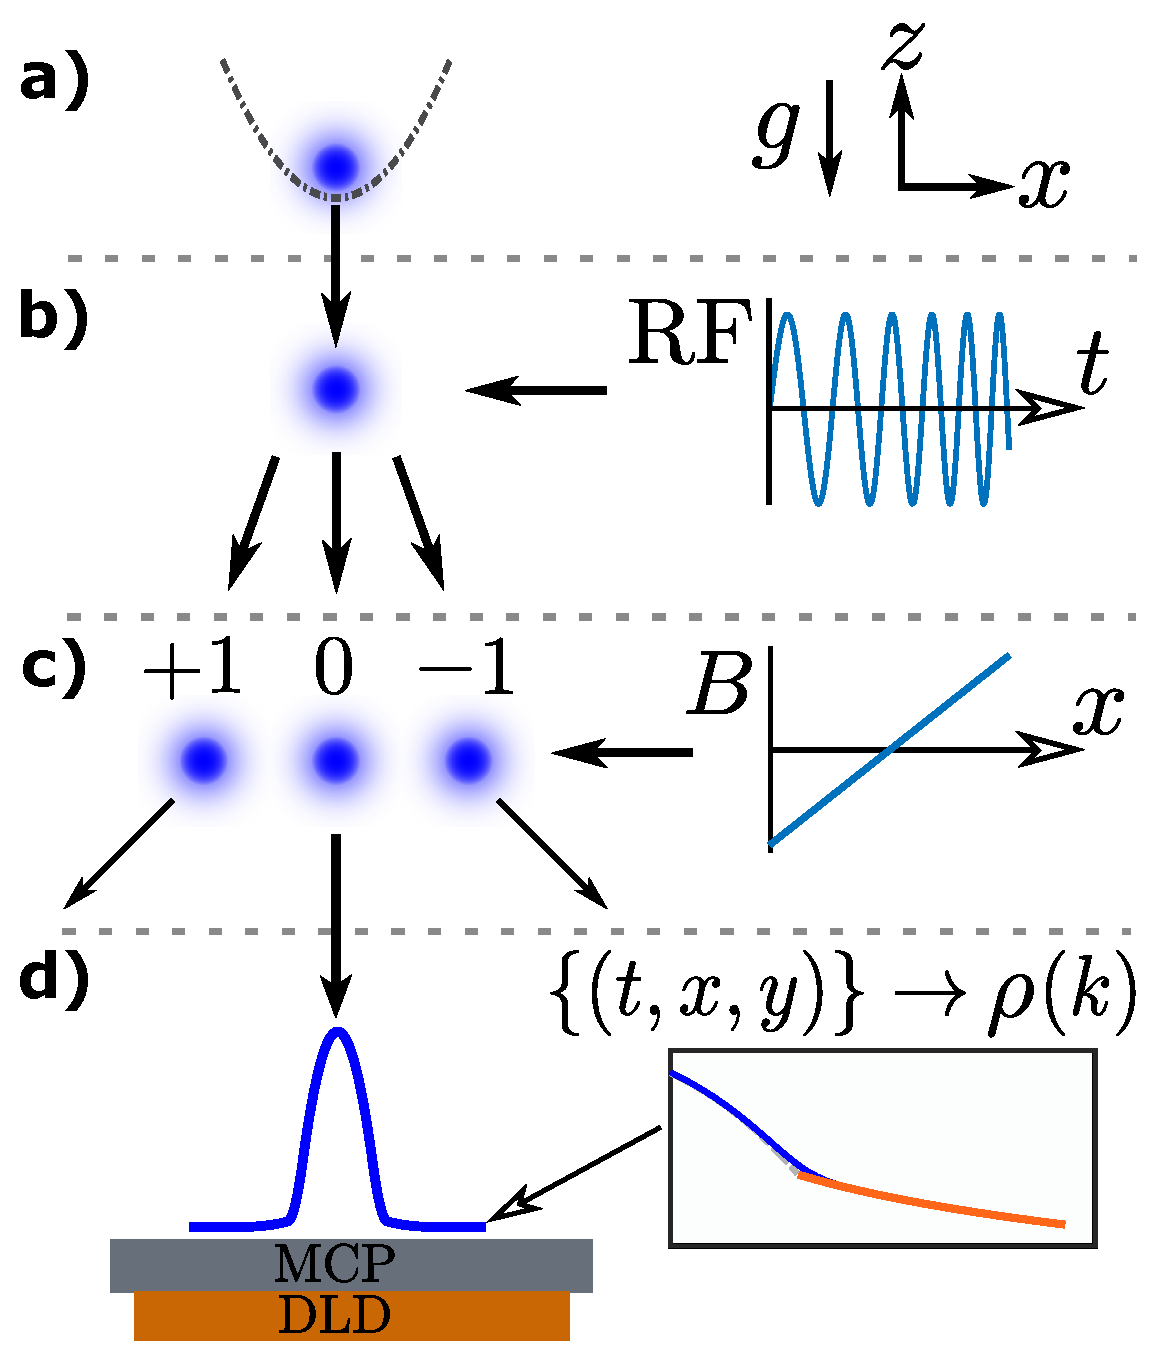
\includegraphics[width=0.4\textwidth]{fig/depletion/main/exp_cartoon}
% % 	    \caption{Sketch of experimental sequence.
% 	A BEC is released from a harmonic trap with (a) and expands during freefall before being split into a superposition of the $m_J\in\{-1,0,1\}$ states (b) by an RF chirp.
% 	A magnetic field gradient separates the clouds (c) ensuring that only the magnetically insentitive $m_J=0$ cloud lands on the detector (d), from which the momentum information is reconstructed.
% 	The quantum depletion lies in the dilute tails at large momentum (inset).}
% % 	    \label{fig:sequence}
% % 	\end{figure}

	


% % \section{Analysis} 

% % 	\begin{figure}[t]
% % 	        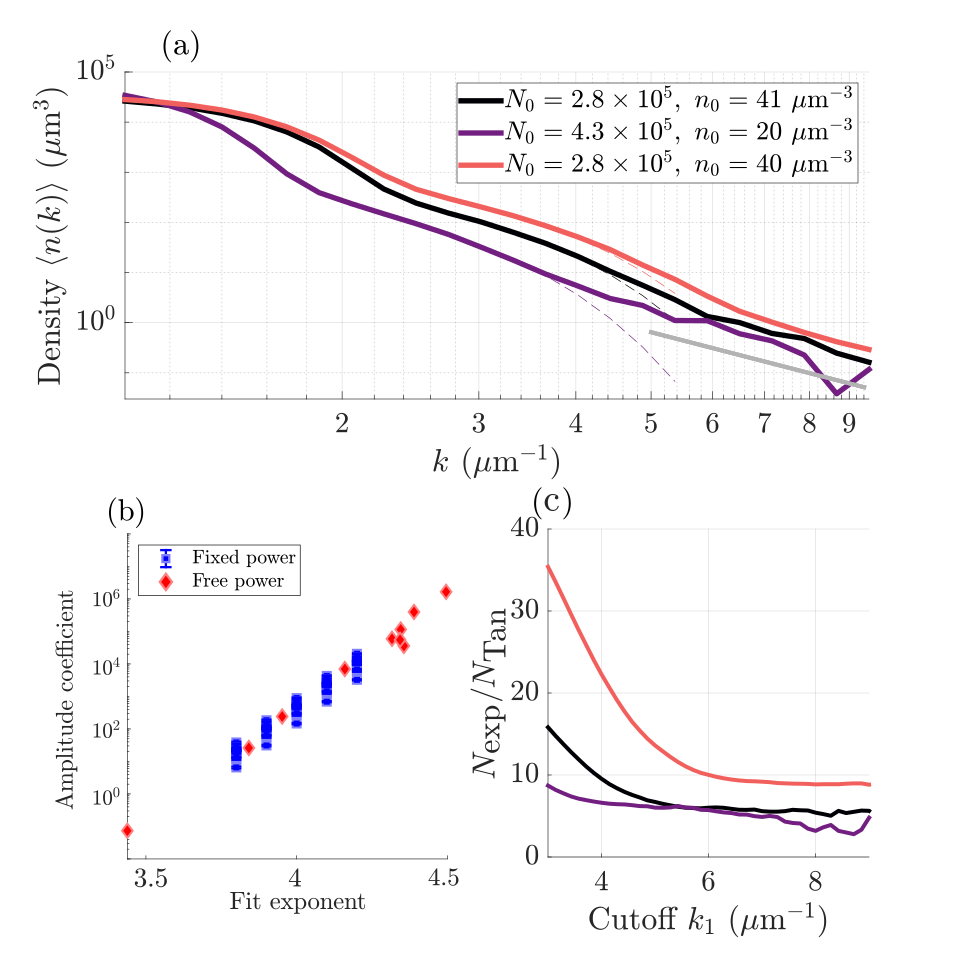
\includegraphics[width=0.5\textwidth]{fig/depletion/main/contact_determination_rev}
% % 	        \caption{The empirical density of particle momenta (a) for different peak densities, where fits to the thermal parts (dashed lines) display exponential decay, which give way to the depletion region, which decays appears to decay with $k^{-4}$ (grey dot-dashed line).
	
% % 	        In (b) we demonstrate the sensitivity of the fitting parameters to constraints in the power law.
% 	Blue squares show the amplitude coefficient $C$ given an exponent $\alpha$ fixed at five values in the range [3.8,4.2], applied to all data sets.
% 	For comparison, leaving $\alpha$ as a fit parameter gives a wide variation in best-fit exponents and scale coefficients.
% % 	        In (c) we show a way around this issue by comparing the number of atoms within the depletion region with the predictions of Eqn.
% 	(\ref{eqn:pred_num}).
% 	We fix $k_2=10\mu\textrm{m}^{-1}$ and $\phi_c=\pi/3$ to define the ROI, and show that $C_\textrm{exp}$ is not significantly dependent on $k_1$ in the depletion region $k\gtrsim6\micron^{-1}$.}
% % 	        \label{fig:cdfplot}
% % 	\end{figure}


% % 	In Fig.
% 	\ref{fig:cdfplot} (a) we show the empirical density $n(k)$ for three representative data collection runs.
% 	The three regimes of the condensate, thermal depletion, and quantum depletion span over five orders of magnitude in density.
% 	The thermal part of the distribution is well fitted by the momentum distribution of an ideal Bose gas,
% % 	\begin{equation}
% % 		n_T(k) = N_T \frac{g_{3/2}\left(\exp(-k^2 \lambda_{dB}^2/4\pi)\right)}{1.202(2\pi/\lambda_{dB})^3}
% % 		\label{eqn:th_fun}
% % 	\end{equation}
% % 	wherein the thermal de Broglie wavelength $\lambda_{dB} = \sqrt{2\pi\hbar^2/(m k_B T)}$  yields an estimate of the temperature $T$ (between 100 and 320 nK (accurate to order 10\%) in our experiments).
% 	Here, $g_{3/2}(\cdot)$ is the standard Bose integral and $N_T$ is the number of atoms in the thermal part.
% % 	The thermal population decays exponentially with $k$, as shown in Fig.
% 	\ref{fig:cdfplot} (a), and hence cannot account for the counts we observe beyond $k\gtrsim 5~\micron^{-1}$.
	
% % \subsection{Issues with analysis of power laws}	

% % 	However, fitting histograms with power-law functions is prone to biased estimates of parameters and drastic underestimation of uncertainties, especially when data is available over less than a couple of decades of dynamic range \cite{Clauset09,Virkar14}.
% 	We first demonstrate some issues with this approach, then discuss our alternative approach.
% % 	If we augment the fit function (Eqn.
% 	(\ref{eqn:th_fun})) with power-law term of the form $C/k^\alpha$, the average exponent of over all runs is 4.2(4).
	
% % 	For comparison, the prior work \cite{Chang16} reported power-law tails with an exponent 4.2(2).
% % 	At first glance, one could simply determine the amplitude of the tails by fixing the exponent to 4, and perhaps achieve better results by using a fit weighting proportional to $k^4$.
	 
% % 	However, as we argue here, there are two issues which preclude such an appealing approach.

% % 	First, in Fig.
% 	\ref{fig:cdfplot} (b) we illustrate how the exponential relationship between the scaling exponent $\alpha$ and the scale coefficient $C$, given the same data.
% % 	% hen fitting a power-law of the form $Ck^{-\alpha}$ to fixed data.
	
% % 	The coefficient $C$ varies over about three orders of magnitude as one uses different exponents $\alpha$ which lie within the range of uncertainties reported here and in the prior work \cite{Chang16}.
	
% % 	For example, fixing $\alpha=4$ in our fits (within the systematic variation) yields a fit amplitude which differs by from the best-fit value by up to a factor of order $100$.
	
% % 	Furthermore, this problem is not captured by the error estimates in the fitting routines: The error bars representing the uncertainty in fit amplitude are smaller than the markers used in Fig.
% 	\ref{fig:cdfplot} (b).
	
% % 	Finally, a linear fit shows that $d \log_{10} C/d\alpha \approx 6.8$, from which we can find the exponent that would yield an amplitude in agreement with Eqn.
% 	(\ref{eqn:pred_scaling}).
	
% % 	This turns out to be approximately 3.9, which is not distinguished with statistical significance from the results of the fitting procedures described here.
	
% % 	Conversely, we can estimate that the best-fit exponents reported in the prior work would lead to scale coefficients a factor of about 23 greater than their conclusions.
	
% % 	This demonstrates that the choice of fit exponent has an outsize influence on the estimate of the corresponding amplitude.
	
% % 	It would be easy to choose $\alpha$ which is not statistically significantly different from the best-fit estimates and arrive at a conclusion which agreed perfectly with the predictions of Eqn.
% 	(\ref{eqn:pred_scaling}), or indeed essentially any tail amplitude one wants.

% % 	Second, a deceptively reassuring result can be found by multiplying the empirical density by $k^4$, observing a flat region, and adding a constant term in an appropriately scaled model of the thermal region (i.e.
% 	Eqn.
% 	(\ref{eqn:th_fun}) multiplied by $k^4$).
	
% % 	In fact, this offers no such recourse.
% % 	Suppose the density decays as some $C k^{-(\alpha+\epsilon)}$: then the scaled density is simply $C k^{-\epsilon}$.
	
% % 	We showed above that a variation of the exponent on the order of a few per cent is both within the systematic error of the fitting procedure and also sufficient to yield drastically different conclusions.
% % 	A variation in $\alpha$ of this size would manifest as a difference of only a factor of order $2^{0.1}\approx1.07$ over the range $5\micron^{-1}\gtrsim k\lesssim10\micron^{-1}$, which is the entire region investigated both here and in the prior work.
% % 	This variation of less than $10\%$ is swamped by the noise in the individual density profiles and is not distinguishable from the run-to-run variation in the power law.

% % 	In sum, there are problems with fitting power laws and it is not clear that the conclusions drawn from such an analysis are insightful even at the best of times.
% % 	In general, determining the exponent of a power law is difficult and requires data over several orders of magnitude in scale \cite{Clauset09,Virkar14}.
% % 	\com{In this case, one could argue that there is a physical rationale for employing $\alpha=4$, but...}
% % 	The preferred statistical tools for analysing power law distributions are maximum likelihood estimators \cite{Goldstein04,Clauset09,Virkar14,Hanel17}, but these are unsuitable here because there are multiple  sources of detection events (discussed further in Appendix A).
	
% % 	Therefore it may not be possible to precisely determine the exponent of a putative power law decay for purposes of the comparison with theory.
	
% % 	We circumvent this issue by using a simpler point of comparison: the number of atoms detected within a region of interest (ROI).
% 	Moreover, we will show that the population of the tails depends on the condensate parameters in agreement with the theory of the contact, albeit up to a constant factor.
	
% % \subsection{Quantifying excess tail amplitude}

% % 	Under the null hypothesis that the \emph{in situ} depletion survives the expansion and escapes the condensate undisturbed, one can integrate Eqn.
% 	(\ref{eqn:pred_scaling}) to predict the expected number of atoms whose wavevector has a modulus in the interval $k\in (k_1, k_2)$, 

% % 	\begin{align}
% % 	\mathcal{N}_\textrm{Tan} &=\frac{\mathcal{C}}{2\pi^2}\left(\frac{1}{k_1}-\frac{1}{k_2}\right)
% % 	\label{eqn:pred_num}
% % 	\end{align}
% % 	 % The noise floor is set by the detector's dark count rate, which contributes an average of less than 1 counts to the region of interest per shot
	
% % 	The null hypothesis can be compared with the experimental results once the bounds of the ROI have been specified (namely, the values $k_1$ and $k_2$, and the solid angle of integration).
% 	We face a tradeoff in the choice of $k_2$ and the minimum elevation angle $\phi_c$ in defining the region of interest.
% 	This is because the field of view of our detector is limited by the 40mm radius of the circular detection surface to $\lesssim5\times 10^6$ m$^{-1}$ in the $(x,y)$ plane, which is only just sufficient to reach past the edge of the thermal region.
% 	The collection volume is maximized for $\phi_c=\pi/3$ rad and $k_2=10^7$ m$^{-1}$, centred on the BEC.
% 	This amounts to an ROI consisting of two vertically oriented conical sections, each with half-angle $\pi/6$, encompassing a total solid angle of $0.13\times 4\pi$ steradians.
	

	
% % 	In Fig.
% 	\ref{fig:cdfplot} (c) we compare the number of detected atoms, corrected for state transfer and detection efficiency, with the predictions obtained from Eqn.
% 	(\ref{eqn:pred_num}) as a function of the lower bound $k_1$ with $k_2=10~\micron^{-1}$ and $\phi_c=\pi/3$.
	
% % 	We consider the average of the quantity $C_\textrm{exp}=N_\textrm{exp}/N_\textrm{Tan}$ over the range $6~\micron<k<10~\micron$, outside the thermal region, as a test statistic for the null hypothesis.
% % 	The uncertainty in a single run is identified as the variance in the estimate over the ROI.
% % 	Averaging over all runs yields an average of 8(1) times as many counts as predicted by Eqn (\ref{eqn:pred_num}), where the final uncertainty is the standard error in the mean and only the most significant digit is shown.
% % 	Thus, while the observed momentum distribution appears consistent with a $k^{-4}$ asymptotic decay, the amplitude of these tails contradicts the null hypothesis of Eqn.
% 	(\ref{eqn:pred_num}) by 5.4$\sigma$.
% 	This would seem to be a count against the interpretation of these tails as a signature of the quantum depletion.
% 	However, we note two pieces of evidence that give weight to this interpretation.
	
% % 	% While at first glance this seems consistent with the fitting procedure, we find that the latter is not stable inasmuch as....	
	
% % \subsection{Consistency in effect size scaling}


% % 	First, the amplitude of the tails scales with $\bar{\omega}$ and $N_0$ in a manner consistent with Eqn.
% 	(\ref{eqn:TotalHarmonicContact}), which can be seen in Fig.
% 	\ref{fig:results_comp}, where we show the estimated contact $C_\textrm{exp}$ obtained by inverting Eqn.
% 	(\ref{eqn:pred_num}).
	
% % 	On one hand, the linear scaling of $C_\textrm{exp}$ with the product $N_0n_0$ is consistent with Eqn.
% 	(\ref{eqn:pred_scaling}).
	
% % 	In fact, this means $C_\textrm{exp}$ scales with $\left(\omega^6 N_0\right)^{1/5}$, i.e.
% 	as predicted by Eqn (\ref{eqn:TotalHarmonicContact}).
	
% % 	Indeed, if we consider the data from each trap configuration separately, the results are also consistent with the same scale factor as above.
% % 	In the absence of another known quantity which exhibits this specific nonlinear scaling relationship, we conclude this line of evidence is supportive of the tails as originating in the quantum depletion.
	
% % 	Second, we find evidence in our simulations (see next section) that the momentum-space signature of the quantum depletion does survive the condensate expansion, and indeed appears in excess of the predicted \emph{in-situ} depletion.
% 	Moreover, several features common to both experimental and simulated momentum distributions emerge, strengthening the identification of the momentum tails with the quantum depletion.
	

% % 		\com{Remarkably, if we do fix $\alpha=4$ then we find fit coefficients that are, on average, 7.8(1.7) times the predicted contact, whereas the fits with free exponents produce a wide range of coefficients, of the order of $4(8)\times10^3$ times the value of the contact calculated using Eqn.
% 	\ref{eqn:pred_scaling}, where the uncertainty is the standard deviation of the fit coefficients.

% % 		In short, it seems that fiddling with the exponent (even by only 0.2 our of 4) is not analytically justified.
% 	This might be ameliorated if there was good physical reason to assume that we are looking at a fourth-power decay, but this is motivated reasoning: In the question of whether or not this is quantum depletion, an almost-matching power law is not a smoking gun, and the sensitivity of the conclusions is remarkable.
% 	More remarkable is the fact that despite these methodological issues, in this specific instance the agreement with a more stable method should not be seen as vindication, but rather as good luck.}


% % 		 Don't seem to have the statistical strength to comment on the istortion of the profile
% % 		Second, we have similar deviation from the power-law distributed momenta in semiclassical simulations.
% 	By simulating the motion of particles with a power-law momentum distribution as they interact with an expanding parabolic mean-field potential in three dimensions, one finds increase in the weight of the momentum tails at small momentum, but the large-$k$ particles are unaffected.
% 	This causes a deviation from the power-law behaviour and a decay slightly faster than $k^{-4}$.
% 	Indeed, a note published by one of the authors of \cite{Chang16} found this effect in 1D \footnote{available via https://web.archive.org/web/20210506045825/https://github.com/rocksonchang/Helium-iPythonNotes/tree/master/20160629\%20-\%20Meanfield\%20kick} and we made similar observations in 3D semiclassical simulations.
% 	Therefore, the exponent slightly greater than 4 is not obviously inconsistent with the population arising from the quantum depletion.
% 	What is surprising is that the amplitude is so much greater than expected, and so we turn to our simulations for further insight.
	
% % 	\begin{figure}[t]
% % 	        \includegraphics[width=0.5\textwidth]{fig/depletion/main/results_comp}
% % 	        \caption{Comparison of simulations and experiments.
% 	The inset is a zoomed view.
% 	 From our empirical data (ED) we determine the empirical contact $C_\textrm{exp}$ which is linear in the product $N_0n_0$ (as predicted by Eqn.
% 	(\ref{eqn:pred_scaling})), but 8(1) times more sensitive (Av) than the prediction by the Tan theory (TT).
% 	The simulated contact of BECs in a cigar-shaped trap (CT) are consistent with (TT) before release and increases after expansion (CE), but by less than the experiment.
% 	A slow relaxation of the tight axes of the cigar trap (CS) leads to a reduction in the simulated contact.
% 	Simulations of a spherical trap (ST) show a negligible increase after expansion (SE).
% 	The prior \mhe result \cite{Chang16} (IO) is shown for comparison (dashed line)}
% % 	        \label{fig:results_comp}
% % 	\end{figure}

% % \subsection{Experimental details}

% % \subsubsection{Trap configuration and calibration}

% % 	We prepared our BECs with via forced evaporative cooling in a harmonic magnetic trap with trap frequencies $(45,425,425)$ Hz and a DC bias stabilized by our auxiliary field compensation coils \cite{Dall07,Dedman07}.
% 	For the tight trap we increased the coil current after the cooling sequence to obtain trapping frequencies $(71,902,895)$ Hz, ramping the field as a sigmoid step function to minimize in-trap oscillations.
% 	Note that the weak ($x$) axis of the trap is horizontal, with tight vertical confinement.
% 	The trap remained on for 150ms before switching the trap off with a $1/e$ time of $\approx38\mu$s.
% 	The condensates were allowed to expand for 2ms before we transferred some of the condensate into the magnetically insensitive $m_J=0$ state via Landau-Zener sweep to prevent distortion by stray magnetic fields.
% 	The RF pulse was created by a  function generator, amplified, and applied to the experiment chamber by a coiled antenna inserted into the BiQUIC coil housing.
% 	The pulse swept from 1.6-2.6MHz over 1ms and was centred on the fine structure resonance between the $m_J$ states.
% 	The transfer efficiencies $\eta_j$ for each of the $m_J = j$ states is discussed in the next section.
% 	The sweep was $10^6$-fold wider than the Doppler broadening of the BEC which ensured uniform transfer at all momenta.
% 	Immediately after the RF sweep, the bias coils are switched off and auxiliary push coils in the vertical (Z) and weak horizontal (X) axes are activated using a fast MOSFET switch to implement a Stern-Gerlach separation of the $m_J = -1,~0,$ and $+1$ pulses.

% % 	We use a Roentdek DLD80 multichannel plate and delay-line detector stack \cite{Manning10} located 859mm below the trap, which registers the arrival times and positions $(t_i,x_i,y_i)$ of each atom, indexed by $i$.
	
% % 	The velocity of each atom relative to the centre of mass of the cloud is calculated by $(v_x,v_y,v_z) = t_{i}^{-1}(x_i-\bar{x},y_i-\bar{y},g_0(\tau^2-t_{i}^{2}))$, where $g_0$ is the local gravitational acceleration and the overbar denotes the within-shot average and $\tau=417$ ms is the time of flight of the centre of mass.
	
% % 	The far-field momentum is thus obtained via $m\textbf{v} = \hbar\kvec$.
% % 	The velocity conversion assumes a point source but carries a negligible error of a few ppm as the in-trap BEC size is smaller than the detector resolution.
	
% % 	The space and time resolution of the detector are 100 $\mu$m and 3 $\mu$s, respectively \cite{Henson18}, and the detector efficiency of $8(2)\%$ was determined from the collection efficiency of correlated atoms on the opposite sides of scattering halos \cite{shin19,shin20,Jaskula10}.
	

% % \subsubsection{Determining transfer efficiency}

% % 	To calibrate the transfer efficiencies, we applied a weaker Stern-Gerlach than for the depletion measurement, resolving each $m_J$ cloud on the detector, as illustrated in Fig.
% 	\ref{fig:frac_cal}.
	

% % \begin{figure*}[!t]
% % 	\begin{center}
% % 		\includegraphics[width=\textwidth]{fig/depletion/main/frac_cal_profile}
% % 		\caption{Determining the RF transfer efficiency.
% 	The time-of-flight profiles of each pulse are resolved (a) by applying a weak Stern-Gerlach pulse during the time of flight.
% 	The pulses are aligned with respect their centre-of-mass (b) and used to determine the pointwise fraction ((c), dotted line).
% 	Detector saturation is evident in the peaks (dashed lines), but not in the thermal tails (solid lines), which are used to compute the transfer efficiency.
% 	Because of its lower flux, the $m_J=-1$ pulse does not show evidence of saturation (d) and is used to determine the thermal fraction.}
% % 		\label{fig:frac_cal}
% % 	\end{center}
% % 	\end{figure*}

% % 	The efficiencies $\eta_J$ cannot be calculated by counting the atoms in each cloud because the detector saturates during the peak condensate flux, but we can compare the thermal parts.
% 	We align each cloud along the time (Z) axis and compute the pointwise fraction of the atomic flux $\phi(t)$ accounted for by each cloud, $\eta_j(t) = \phi_j(t)/\sum_j\phi_j(t)$, as depicted in Fig.
% 	\ref{fig:frac_cal}.
% 	The ratio of densities between the clouds is roughly constant in the thermal part, indicating the absence of important saturation effects and a spin transfer that is independent of $k$.
% 	The fraction of the original cloud transferred into each $m_J$ state is determined by taking the average $\langle\eta_j(t)\rangle$ over the thermal tails.
% 	We find these efficiencies are approximately 74\%, 24\%, and 2\% in all runs for the $m_J=+1$, 0, and -1 states, respectively.
	
% % 	While the $m_J=0$ and $m_J=1$ clouds clearly saturate the detector, the small fraction ($\approx2\%$) of the atoms transferred to the $m_J=-1$ state does not (Fig.
% 	\ref{fig:frac_cal} (d)).
% 	A bimodal fit to the condensed and thermal parts, plus constant background, yields an estimate of the thermal and condensed fractions.
	


% % % \subsection{Determination of thermal fraction}
	

% % % 	\begin{figure}[!h]
% % % 	\begin{center}
% % % 		\includegraphics[width=0.8\textwidth]{fig/depletion/main/m1_frac_anal}
% % % 		\caption{Comparison of thermal fits in the unsaturated $m_J=-1$ pulse including 138 shots.
% 	The weak (X) and strong horizontal (Y) trapping axes are shown in (a) and (b), respectively.
% 	\org{would be helpful to label $v_x$ and $v_y$ to make it self-evident at 1st glance.} Both projections display a bimodal peak, with the condensate (dotted lines) and thermal parts (thick solid lines) easily distinguished.
% 	Fitting a Gaussian profile (thin solid line) to the velocity distribution of the thermal part yields the thermal number and temperature.
% 	Subtracting the fit leaves the condensate profile (c) which can be \blu{\dots something\dots} yields the condensed number.}
% % % 		\label{fig:thermal_frac}
% % % 	\end{center}
% % % 	\end{figure}



% % \subsubsection{Analysis of spin transfer measurements}

% % 	In early tests of our measurement sequence we noticed a contamination of the signal by spurious counts.
% 	We inferred these were remnant counts from the $m_J=+1$ cloud as they were still visible when we ran an experimental sequence without the Landau-Zener transfer.
% 	This contamination appeared in a particular region of our detection image, illustrated in Fig.
% 	\ref{fig:spinpop}.
% 	As such we were able to correct for it by subtracting their contribution from the counts collected during measurement shots.
% 	Generally, fewer atoms can be attributed to this noise ($\leq~1$ atom per shot, on average) than would be required to explain the discrepancy described in the main text ($5-10$ counts per shot).
% 	While the cause of the cross-contamination is unclear, we observe that the count density outside the region of interest is similar in both the shots with the RF pulse and those without.
% 	We hypothesize that the remnant counts are atoms transferred into the $m_J=0$ state by non-ideal behaviour of the Stern-Gerlach pulses.
% 	We note that only about one in a million atoms from the $m_J=1$ cloud present in this manner in a given shot.

% % 	As mentioned in the main text, the presence of these counts also prevents a straightforward application of a maximum-likelihood estimator (MLE) to determine parameters of the power-law region.
% 	The basic principle of the MLE is to assume a functional form for the probability distribution $p(x|\theta)$ underlying the observed data $x$, and dependent on some parameters $\theta$; the zero of the derivative of the \emph{likelihood} function $L(\theta|x)$ with respect to the parameters $\theta$ then yields the most-probable parameter values given a set of observations $x$.
% 	In our context, one can assume a functional form for the probability distribution underlying atomic detection events (via a wavefunction ansatz).
% 	The detector dark count rates can also be incorporated by assuming a uniform distribution, although this necessitates a cumbersome procedure to retain proper normalization.
% 	Such an analytical treatment does not readily permit the inclusion of an empirical density estimate which itself includes the aforementioned dark count rate.
% 	Instead, we opt for the simpler approach described in the main text.

% %     \begin{figure}[!b]
% % 	\begin{center}
% % 		\includegraphics[width=\columnwidth]{fig/depletion/main/spinpop}
% % 		\caption{Measured contribution of the detector dark counts and spurious spin counts to the time-of-flight profile.
% 	We accounted for the pulse at around 550ms and subtracted it from the measured profiles when computing the contact.
% 	After removing this background term, the density profiles above and below the condensate agree, indicating convergence on the true signal.
% 	For reference, the peak flux of the $m_J=0$ condensate is about a thousandfold greater than the peak shown here.}
% % 		\label{fig:spinpop}
% % 	\end{center}
% % 	\end{figure}

% % 	% \begin{figure}[!h]
% % 	% \begin{center}
% % 	% 	\includegraphics[width=\textwidth]{fig/depletion/main/profile_overlay}
% % 	% 	\caption{Comparison of average time-of-flight profiles over a single data run for the quantum depletion measurement shots (blue, 871 shots), transfer efficiency calibration (black, 112 shots), detector dark counts (red, 871 shots), and spurious counts (dot-dash, 895 shots).
% 	The time window bounded by $|k|\leq 10\mu$m is indicated with dotted lines.
% 	Shaded area is the standard error over the entire run.}
% % 	% 	\label{fig:tof_profile}
% % 	% \end{center}
% % 	% \end{figure}




% % % Note that the temps disagree between axes, but within axes between clouds they are consistent(....ish).
% 	This means we can use the profile ratio method, which is also consistent with comparing the thermal number from the fits.
% % % Perhaps comment on the thermal-subtracted part; the TF profile should have a sharp cutoff, but the smooth edges are suggestive evidence of this roll-off

% % % \begin{figure}
% % % 	\centering
% % % 	\includegraphics[width=0.5\textwidth]{fig/depletion/main/counts_per_run}
% % % 	\caption{Number of counts detected in the region of interest in the depletion measurement (a), the spin mixing calibration (b), and the dark count calibration (c).
% 	An average of 3.0(5) counts were detected in the ROI in the spin-mixing calibration shot, and the background count rate was 0.4(2) counts per shot.
% 	Separate lines indicate separate \emph{runs}, i.e.
% 	sequences of shots with fixed parameters.}
% % % 	\label{fig:num_counts}
% % % \end{figure}


% % \subsection{Peak density calibration}

% %     The quantum depletion and contact are both predicted to depend solely on the condensed number and trapping frequencies via the condensate density, hence it is important to determine both quantities accurately.
% 	In the Thomas-Fermi approximation, the peak density of the condensate can be written as $n_0 = \mu/g$, where $\mu$ is the chemical potential, $g=4\pi\hbar^2a_{1,1}/m$ is the effective interaction strength, $m\approx6.6\times10^{-27}$ kg is the atomic mass, and $a=7.512$ nm is the s-wave scattering length between pairs of atoms in the $m_J=1$ state \cite{Moal06}.
% 	The sole experimental parameters in the expression for the peak density (Eqn.
% 	\ref{eqn:n0}) are $\bar{\omega} = \left(\omega_x\cdot\omega_y\cdot\omega_z\right)^{1/3}$,  the geometric trap frequency, and $N_0$, the number of atoms in the condensate.
% 	During these calibration runs we simultaneously determine the total atom number $N$ and trap frequency $\bar{\omega}$ in a single shot using a pulsed atom laser and use the thermal fraction (as below) to determine the condensed number $N_0$.
	

% % 	The pulsed atom laser consists of a series of Fourier-broadened RF pulses centred on the minimum Zeeman splitting in the trap.
% 	The pulse transfers atoms in the trap to the untrapped $m_J=0$ state with an approximately constant transfer rate across the cloud.
% 	We outcouple approximately 2\% of the atoms per 100$\mu$s pulse for $\approx$200 pulses, which eventually depletes the entire trap.
% 	The atom laser thus prevents the detector from saturating and allows an accurate determination of the atom number, up to a factor of the quantum efficiency.
% 	We determine the trapping frequencies by inducing centre-of-mass oscillations with a magnetic impulse, and finding the oscillation period from the atom laser pulses \cite{henson18ML}.



% % \section{Numerical simulations}
% % \label{STAB}

% % 	We performed simulations of the BEC expansion from harmonic traps using the first principles STAB method \cite{Deuar11,Kheruntsyan12}.
% 	The simulations included a cigar-shaped trap (marked CT in Fig.
% 	\ref{fig:results_comp}) with parameters matched to the experimental conditions.
% 	The in-trap state was consistent with the adiabatic sweep theorem before release from the trap.
% 	Following expansion from the cigar trap (CE in Fig.
% 	\ref{fig:results_comp})), the simulated tail amplitude increased and stabilized within a few hundred microseconds, much sooner than the 2ms delay between the trap release and application of the rf and Stern-Gerlach pulses.
% 	Fig.
% 	\ref{fig:time_dep_theory} shows time evolution of the tail amplitude for the simulated traps using the same ROI as the experimental setup.
% 	 In this configuration the steady-state value of the momentum tails was a factor of 1.64(9) above the predictions of Eqn.
% 	(\ref{eqn:pred_scaling}).
	

% % 	To understand the disagreement with earlier theory \cite{Qu16}, which predicted no depletion survival, we also investigated the effect of adiabatic expansion on the in-trap depletion by simulating a slow decrease of the transverse trapping frequencies by a factor of two (CS), and found that the in-trap contact decreased roughly as predicted by Eqn.
% 	(\ref{eqn:pred_scaling}) in these instances --- see the dashed line in Fig.~\ref{fig:time_dep_theory}.
	

% % 	We also found that the factor of disagreement (i.e.
% 	$C_\textrm{sim}/C_\textrm{Tan}$) between Eqn.
% 	(\ref{eqn:pred_num}) and the simulated tails depends on the angle choice of cutoff angle $\phi_c$.
% 	Put another way, the momentum distribution in the simulations is anisotropic and takes the form $f(\theta,\phi)/k^4$.
% 	We note that the average of an angle-dependent power law decay over a region $\Omega$ is simply $\langle f(\theta,\phi)\rangle_\Omega/k^4$, preserving the power-law behaviour.
% 	We find a similar effect in the experimental data as well, albeit with low statistical significance owing to the small signal-to-noise.
% % 	Specifically, we find that $C_\textrm{exp}$ is larger for smaller collection regions that are more tightly concentrated about the vertical (strong) trapping axis, whereas larger collection angles (including areas closer to the weak axis) produce a lower $C_\textrm{exp}$.
% % 	We quantify this effect in Tab.
% 	\ref{tab:angle_dep} and propose physical origins of our observations in the next section.
	

% % 	\begin{figure}[t]
% % 	        \includegraphics[width=0.5\textwidth]{fig/depletion/main/time_dep_theory}
% % 	        \caption{Simulations of condensates released from a cigar-shaped trap show an increase in contact after the trap release, stabilizing after a time on the order of $1/\omega_x$, several hundred $\mu$s.
% 	The relative difference between in-trap and expanded contact increases with the density of the condensate.
% 	For comparison, the experimental control pulses are implemented after 2ms of expansion.
% 	In contrast, when the transverse trapping frequencies are reduced by half (dotted line), the in-situ contact relaxes.}
% % 	        \label{fig:time_dep_theory}
% % 	\end{figure}

% % 	\begin{table}[b]
% % 		\begin{tabular}{c c c}
% % 			\hline\hline
% % 			Half-angle &	$C_\textrm{exp}/C_\textrm{Tan}$ &	$C_\textrm{sim}/C_\textrm{Tan}$\\
% % 			\hline
% % 			10	&	9.3(3.3) &	2.2(3)\\
% % 			20 	&	8.7(1.8) &	1.9(2)\\
% % 			30	&	8.0(1.3) &	1.6(1)\\
% % 			\hline\hline
% % 		\end{tabular}
% % 		\caption{The excess of detection events over the expected number depends on the choice of angular bounds for the ROI.
% 	We show the average factor of disagreement between experimental and predicted counts for three half-angles defining the two vertically oriented conical sections.
% 	For comparison, we show the factor of disagreement for the $C_\textrm{sim}/C_\textrm{Tan}$simulated case where $n_0=44~\micron^{-3}$.}
% % 		\label{tab:angle_dep}
% % 	\end{table}

% % % \include{sim_part}


% % \section{Discussion}

% % 	We interpret these results as an indication that the depleted atoms are accelerated by the non-uniform mean-field energy of the condensate during the expansion.
% % 	In detail, after a quench into the free particle regime, the condensate expands hydrodynamically on timescales of $1/\omega$.
	
% % 	This is an adiabatic process for the low momentum depletion, whereby some depleted atoms are absorbed back into the condensate in agreement with \cite{Qu16}.
% % 	However, the characteristic time for reabsorption is $\hbar/gn_0$, slow enough that quasiparticles in the particle branch of the Bogoliubov dispersion have sufficient velocity to escape the expanding cloud without being reabsorbed and thus transition to free atoms.
	
% % 	This effect contributes to the disagreement between \emph{in situ} and measured tail amplitudes, hence $C_\textrm{exp}$.

% % 	Moreover, an atom inside the BEC experiences an effective force from the gradient of the mean-field potential $\textbf{F} = -4\pi\hbar^2a \nabla  n(x)/m$.
	
% % 	This endows escaping depleted particles with a greater momentum, increasing the weight of the tails in the far-field.
	
% % 	This effect is exacerbate in light atoms like $^{4}$He: because the acceleration scales with $1/m^2$, it would be suppressed by a $\sim500$-fold in $^{87}$Rb experiments \cite{Makotyn14}.
	
% % 	Further, it is much easier for depletion atoms to escape and be accelerated in the transverse x-y directions from an elongated cloud because the distances $R_{TF}=\frac{1}{\omega}\sqrt{2gn_0/m}$ are reduced by $\bar{\omega}/\omega_{x,y}$, whereas the initial mean depletion velocities \textit{in situ} $v\sim \sqrt{2gn_0/m}$ are isotropic.
% % 	Indeed, spherical clouds (SE) exhibit a much weaker effect than the elongated clouds (CE) owing to the longer escape time.
% % 	Furthermore, we find some evidence that this anisotropic feature is present in our experimental data.
	
% % 	The hypothesis that this conjunction underlies the observed effects is further supported by our simulations: We observe a decrease in the total number of depleted particles (reabsorption) and a simultaneous increase of the large-k population (forcing).
	
% % 	This constitutes a partial explanation of the experimenal findings too, exhibiting important similar features including the anisotropic distribution and nonlinear scaling consistent with the quantum depletion.
	

% % 	\com{Two factors to address: Detector efficiency and the Landau-Zener transfer}


% % 	However, a mystery remains: Why is the excess depletion some four times greater than accounted for by this picture? This issue should be resolved in order to interpret far-field observations in terms of the in-trap physics of interest.
	
% % 	This question invites complementary studies of the \emph{in situ} depletion in \mhe BECs.
	
% % 	The cause of the contact anomaly could be elucidated by determining whether it originates in the trapped condensate, or is generated during the trap release and expansion.
	
% % 	Such an investigation requires an \emph{in situ} probe of the contact, such as RF spectroscopy or Bragg spectroscopy.
% % 	The latter may be the most fruitful of the two simply because of the difficulty of interpreting the results from the former, which we sketch here.
	
	
% % 	The basic principle of RF contact spectroscopy is to apply a monochromatic RF probe which is detuned from the resonance between two spin states, coupling atoms in the initial spin state to an untrapped channel.
	
% % 	One then performs a differential measurement of the atom number and expects the signal strength to scale as $\omega_\textrm{RF}^{3/2}$ with the detuning from the RF resonance.
% % 	The loss rate is also proportional to the difference of reciprocal scattering lengths $\Gamma\propto(1/a_\textrm{i,i}-1/a_\textrm{i,f})$ between pairs of atoms in initial-initial ($a_{i,i}$) and initial-final ($a_{i,f}$) spin states \cite{Braaten10,Wild12}.
	
% % 	For He$^*$ (spin 1) the scattering lengths $a_{1,1}$ and $a_{1,0}$ are identical \cite{Leo01}, rendering the preferred $m_J=1-m_J=0$ transition unusable.
	
% % 	On the other hand, $a_{1,-1} = 3/7 a_{1,1}$ \cite{Vassen16}, and the singlet transition can be driven without populating the $m_J=0$ state.
	
% % 	In principle this could produce a detectable flux of atoms to perform sensitive in-trap contact measurements, however, collisions in the $^1\Sigma_{g}^{+}$ channel have large Penning ionization rates which lead to significant trap losses \cite{Leo01}.
	
% % 	The ionization products would be detectable by in-vacuum channel electron multipliers but require theoretical work to disentangle from the spectroscopic signal.
	
% % 	Further, while other atomic species offer Feshbach resonances by which to tune the inter-species scattering length (and hence signal or ionization rate), \mhe has no such feature.
	
% % 	While such a measurement is not \emph{prima facie} impossible, Bragg spectroscopy may yield more readily comprehensible results.

	
% % 	\section{Conclusion} 

% % 	Our work expands the growing suite of far-field investigations of quantum depletion \cite{Cayla20,Chang16} and confirms that quantum depletion can, remarkably, survive past the lifetime of its original condensate.
% 	Our findings clarify that how the depletion can be visible in the far-field momentum distribution here and in earlier experiments, and that the hydrodynamic approximation does not capture sufficient short-wavelength information to make detailed predictions about the high-momentum behaviour.
% 	We thus find a partial explanation for the deviation of the far-field distribution from both the predicted in-situ depletion and the hydrodynamic reabsorption: The interplay between coherent absorption of Bogoliubov excitations and the dispersal of the chemical potential into kinetic energy, to which helium is particularly sensitive, result in a growth of the $k^{-4}$ tails of the momentum distribution during freefall.
% 	It would be informative to determine whether this discrepancy originates in the trapped condensate or is due to some unknown non-equilibrium effect during expansion.


% % 	\section{Acknowledgements} We Would like to thank David Clement, Raphael Lopes, Jean Dalibard, and Karen Kherunstyan for their helpful discussions.
% 	This work was supported by Australian Research Council (ARC) Discovery Project Grants No.
% 	DP160102337 and No.
% 	DP190103021.
% 	S.
% 	S.
% 	H was supported by DECRA DE150100315,  J.A.R., D.
% 	K.
% 	S.
% 	by the Australian Postgraduate Award (APA), and K.F.T.
% 	by the Australian Government Research Training Program (RTP) Scholarship.
% 	The simulations by P.
% 	D.
% 	were supported by National Science Centre (Poland) grants No.
% 	2018/31/B/ST2/01871 and 2012/07/E/ST2/01389.

% % \nocite{Manning10,Henson18,shin19,shin20,Jaskula10,Dall07,Dedman07,Moal06,henson18ML,PethickSmith,braaten10,wild12,Leo01,vassen16,Deuar11,Kheruntsyan12,Drummond80,Deuar07,Sinatra00,Kheruntsyan12,Deuar11,Krachmalnicoff10,Lewis-Swan14,Lewis-Swan15,Deuar13,Deuar14,nstab-longpaper,Drummond80,Deuar11,tcorr,Deuar13,FINESS-Book-Ruostekoski,FINESS-Book-Sinatra,Martin10a,Martin10b,Sinatra02,Norrie06,Deuar11,DeuarPhD,Drummond20,stob,nstab-longpaper}

% % \bibliography{bibliography}
% % \appendix
% % %\section*{Supplementary Materials}

%\comment{sections just dumped from main text for now - clean up later}



%Our bespoke software interfaces with the LabView control environment and loops over a sequence of experiments, consisting in this case of: Atom number calibration, Trap frequency calibration, and RF transfer efficiency, followed by 10 data collection runs.

%To calibrate the atom number, we used an RF pulse sequence to create a pulsed atom laser with intensity well below the saturation threshold of our delay-line detector. We corrected the number of detected atoms to account for the quantum efficiency ($\sim$8\%) of our detector. 
%\comment{Should use QD measurements to compute condensate/thermal fraction relative sizes and further improve $N_0$ measurement}.
%\comment{how does this compare to our trap binning? What is the uncertainty of the QE?}

%Together with the atom number, a measurement of the centre-of-mass motional frequencies allowed us to compute the peak density of the condensate. We measured the trap frequency by transient magnetic field to the trapped condensate for $\sim 150\mu s$, forcing centre-of-mass motion in the lab frame. We used the same pulsed outcoupling scheme as in the number measurement, and measured the  centre-of-mass momentum of the cloud at the time of each pulse. Our outcoupling frequency is well below the natural frequency of the confining potential so we used a subsampled reconstruction method to recover the trap frequency. Prior to running experiments we varied the outcoupling pulse frequency to determine in which Nyquist zone the actual trap frequency lies relative to our sampling frequency. We can then obtain the trap frequency to within precision X in a single shot of the experiment by taking a Fourier transform of the centre of mass motion.

%Our calibration sequence provided accurate number and peak density measurements along with the condensate profile. We verified the spherical symmetry of the thermal and depleted fractions, and so compute the momentum density by an average over a large section of the momentum distribution. 

%We verified the fitting method by analysing a test data set of known parameters, which was generated by the Metropolis-Hastings algorithm, and find the method recovers the test set parameters within a factor less than our experimental uncertainties.  


%There may still be errors in the analysis. The fitting procedure apparently produces a good fit, but it may be possible to get indistinguishable or better fits by fixing the exponent of the power law to be some $\alpha\neq 4$. This would challenge the assertion that the cause of the observed profile is in fact quantum depletion.  Assuming the observed data does follow a power law, statistical fluctuations in the high-momentum region become amplified by the $k^4$ scaling procedure and could introduce further error in the estimated Tan constant. \comment{Y-error bars are computed in a fairly ad-hoc way, so ours and Chang may be drastically under-reported...)}Reliably estimating the parameters of a power-law distribution is nontrivial\cite{Clauset2009}, and the robustness of the fitting method above has not been exhaustively tested. The LDA prediction is essentially that the single-particle wavefunctions, hence the single-particle probability distribution over momentum, are affected by many-body effects. One computes the single-particle probability density by dividing the condensate density by the number of particles (hence the $N_0$ term in the LDA), and then the problem of extracting the contact parameter from the data is an exercise in statistical parameter estimation. As shown by Clauset et al \cite{Clauset2009}, fitting these functions tends to produce incorrect estimates of parameters. The method outlined in Clauset was proven to asymptotically converge with probability 1 to the correct fit parameters of a power law distribution, but would need to be extended to derive a maximum likelihood estimator for a power law overlaid on a constant background.


% % \end{document}


% % \begin{abstract}

% % Measurements of Tan's contact in expanding condensate conflict with predictions of the \emph{in situ} quantum depletion.
% 	It is unclear how the depletion survives without a condensate, and even appears stronger in the far-field than before the trap release.
% 	We confirm experimental observations of a power-law decay in the far-field, consistent with the survival of the quantum depletion.
% 	Simulations of our experiment support this conclusion and provide a partial explanation.
% 	A gap between the numerical and empirical results is an open question obstructing studies of quantum depletion in the far field.
% % % max 600chars for PRL
% % % \end{abstract}

% % % \maketitle

% % % \section{Introduction} 
% % A profusion of work on quantum degenerate matter is motivated by the promise of the prototypical coherent phenomenon, superfluidity.
% 	The underlying mechanism of superfluid formation is the Bose-Einstein condensation of collective excitations, which was realized by Bogoliubov \cite{Bogolubov47}.
% 	This finding is of broader importance because the BEC and BCS regimes of supercondictivty are characterized by condensation of molecular dimers and of Cooper pairs, respectively.
	

% % Bogoliubov formulated the problem of a homogeneous system of interacting bosons in terms of a free Bose gas of collective excitations, constituted by pairs of particles with opposite momenta \cite{vogels02}.
% 	The thermal population of quasiparticle modes produces the normal component of a superfluid, while the zero-point population, called the \emph{quantum depletion}, accounts for the large-momentum part of the wavefunction.
% 	The Bogoliubov spectrum exhibits a crossover from wavelike phonon modes to single-particle excitations at momenta larger than the speed of sound in the condensate \cite{steinhauer03}, but this description breaks down in strongly interacting systems \cite{lopes17_quasiparticle} whereas the Tan relations remain valid in the strongly-correlated regime.

% % In a modern addition to the theories of quantum matter, Tan explained how s-wave contact interactions modify the short-range pair correlation function and manifests as a power-law decay in the momentum density \cite{tan08_energetics,tan08_momentum,tan08_virial}.
% 	The contact underpins several universal relations between many-body features and microscopic information in aribitrary spin mixures at any density, temperature, and geometry \cite{combescot09,braaten08,braaten11,werner12_boson,werner12_fermion}.
% 	Emerging evidence for analogous relations in p-wave scattering \cite{luciuk16} and three-body interactions \cite{fletcher17} hints at the prospect of new systematic ways to design thermodynamic features by tailoring the interactions between particles.
	

% % Two defining properties of Tan's contact, known as the adiabatic sweep theorem \cite{tan08_momentum} and generalized virial theorem \cite{tan08_virial}, have been decisively verified via radio spectroscopy \cite{baym07,punk07,braaten10} of degenerate Bose \cite{wild12} and Fermi gases \cite{stewart10,sagi12}.
% 	Bragg spectroscopy has revealed the universality of scaling relations for the pair correlation function \cite{kuhnle10} and the behaviour of the contact across the superfluid phase transition \cite{kuhnle11,mukherjee19,carcy19}, yielding benchmarks for descriptions of strongly-correlated gases \cite{rakhimov20}.

% % The Bogoliubov theory has also yielded accurate predictions of the quasiparticle spectrum \cite{lopes17_quasiparticle,vogels02} and of the depleted population in ultracold atomic Bose-Einstein condensates \cite{xu06,lopes17_depletion} and exciton-polariton condensates in solid substrates \cite{pieczarka20}.
% 	The Bogoliubov spectrum exhibits a crossover from wavelike phonon modes to single-particle excitations at momenta larger than the speed of sound in the condensate \cite{steinhauer03}, but this description breaks down in strongly interacting systems \cite{lopes17_quasiparticle}.
% 	However, detailed study of the quantum-depleted tails of the momentum distribution has been challenging to date because the tails are beneath the noise floor of optical imaging techniques.
% 	A previous experiment sought to use a Feshbach resonance to produce a visible depleted fraction \cite{makotyn14}, but found that the momentum distribution saturated during expansion and did not display a power-law tail.
% 	This was because many-body effects shielded condensed atoms from excitation into the normal component \cite{kira15_hyperbolic,kira15_coherent}.


% % In contrast, another experiment found unexpectedly large momentum tails in the far-field of a Helium BEC released from a harmonic optical trap \cite{chang16}.
% 	This is particularly surprising because conventional wisdom argues that the density decreases adiabatically during expansion \cite{xu06}, justifying treatment with a hydrodynamic approximation wherein the tails are predicted to vanish \cite{qu16}.
% 	Instead, the study \cite{chang16} found momentum tails far stronger even than expected in the cloud before release.
% 	This contradiction implies that either helium condensates violate the minimal assumptions of Tan's theory of the contact \cite{tan08_energetics,tan08_momentum,tan08_virial}, or that far-field momentum measurements are not a straightforward means of examining the quantum depletion even in weakly interacting gases.
% 	It is important to verify and overcome this obstacle, as such measurement could play a central role in studying the microscopic physics of superfluids with ultracold gases.

% % To this end, we revisit the measurement of the momentum distribution of a helium condensate expanding from a harmonic trap.
% 	We conducted experiments using an independent apparatus and analysis, covering a range of densities twice as large as in the prior work \cite{chang16}.
% 	We observe power-law tails in the far field whose amplitude significantly exceeds the predictions of the \emph{in situ} depletion, corroborating the prior work.
% 	Our measurements are complemented by simulations of the time-dependence of the momentum distribution using a stochastic Time-Adaptive Bogoliubov (STAB) method in the positive-P framework \cite{Deuar11,Kheruntsyan12,SOM}.
% 	These show that the non-adiabatic release of the trap is responsible for survival of the depletion, and that the depleted particles acquire additional kinetic energy from the mean-field energy of the condensate during the subsequent adiabatic expansion.
% 	These factors result in an amplification of the momentum tails relative to the \emph{in situ} values and are not captured in the hydrodynamic approximation.
% 	However, quantitative disagreement between our simulations and experimental data rule out the release energy as a complete explanation for the observed excess counts.
% 	We conclude by suggesting an informative complementary approach.
	

% % \section{Experiment} Our experimental sequence, depicted schematically in Fig.
% 	\ref{fig:sequence}, began with BECs with between $2\times 10^5$ and $5\times 10^5$ $^4$He atoms polarized in the $\metastable(m_J=1)$ state and cooled to $\sim$ 300 nK by forced evaporative cooling in a harmonic magnetic trap generated by field coils in a Bi-planar Quadrupole Ioffe configuration \cite{Dall07}.
% 	The metastable $\metastable$ state, denoted He$^*$, which is 19.8eV above the true ground state \cite{Hodgman09}, enables single-particle detection in the far-field regime and thus affords direct access to microscopic momentum information.
% 	The use of a multichannel electron multiplier in combination with a delay-line detector (MCP-DLD)  \cite{Manning10} has permitted the observation of many-body momentum correlations \cite{Hodgman11,Dall13} and Hanbury Brown-Twiss bunching of both condensed \cite{Schellekens05,Jeltes07,Manning10,Dall11} and quantum depleted atoms \cite{cayla20}.

% % Investigations of the quantum depletion in \mhe are challenging because the absence of a known Feshbach resonance precludes control over the contact $\mathcal{C}\propto(a N_0)^{7/5}\bar{\omega}^{6/5}$ via the scattering length.
% 	We therefore test the prediction from Eqn.
% 	\ref{eqn:mom_dist} by varying the density of the gas, $n\propto\left(N_{0}\bar{\omega}^3\right)^{2/5}$.
% 	We used two trap configurations with geometric frequencies $\bar{\omega} = 2\pi \cdot201$ rad Hz $\bar{\omega} = 2\pi \cdot393$ rad Hz, and varied the endpoint of the RF evaporation ramp to adjust the number of atoms in the condensate.
% 	We interleaved the measurements just described with calibrations to determine the shot-to-shot variation in atom number, trapping frequencies, magnetic state transfer efficiency $\eta_0$, and noise contributions (see supplementary materials \cite{SOM} for more details).

% % After the trap is switched off, we transferred about one quarter of the atoms to the magnetically insensitive $m_J=0$ state with a radio-frequency (RF) Landau-Zener sweep to avoid distortion by stray magnetic fields.
% 	We deflected the $m_J=\pm 1$ clouds outside the detector field of view by implementing a Stern-Gerlach scheme immediately after the RF pulse.
% 	The atoms then ballistically expanded during the $\approx420$ ms freefall to the MCP-DLD detector $\approx850$ mm below the trap.
% 	The atomic velocity components in the in-plane $v_x$, $v_y$ and vertical $v_z$ directions were reconstructed from the $(x,y)$ position and the time-of-flight of individual atom detection events.
	


% % \begin{figure}[b]
% %     \includegraphics[width=0.4\textwidth]{fig/QD/exp_cartoon}
% %     \caption{Sketch of experimental sequence.
% 	A BEC is released from a harmonic trap (a) and expands during freefall before being split into a superposition of the $m_J\in\{-1,0,1\}$ states (b) by an RF chirp.
% 	A magnetic field gradient separates the clouds (c) ensuring that only the magnetically insentitive $m_J=0$ cloud lands on the detector (d), from which the momentum information is reconstructed.
% 	The quantum depletion lies in the dilute tails at large momentum (inset).}
% %     \label{fig:sequence}
% % \end{figure}


% % \begin{figure}[b]
% %         \includegraphics[width=0.5\textwidth]{fig/QD/contact_determination}
% %         \caption{The empirical density of particle momenta (a) for different peak densities, showing the transition between the condensed, thermal, and depletion regions (indicated for $n_0=20~\mu\textrm{m}^{3}$ with dotted lines).
% 	The number of atoms with wavevector $k\in\{k_1,k_2\}$ within the depletion region yields an estimate of the contact via Eqn.
% 	(\ref{eqn:c_est}).
% 	Fixing $k_2=10\mu\textrm{m}^{-1}$, we show $C_\textrm{est}$ as a function of the cutoff $k_1$ (b), which behaves consistently with a $k^{-4}$-like scaling of the momentum distribution.
% 	For each run we choose the $k_1$ at which $C_\textrm{est}$ is the most stable.}
% %         \label{fig:cdfplot}
% % \end{figure}

% % \section{Results} 
% % The single-particle detections can be used to construct an estimate of the far-field momentum density.
% 	However, estimating parameters of power-law distributions by fitting histograms is prone to bias and underestimation of uncertainties, especially when data is available over less than a decade of dynamic range \cite{clauset09,virkar14}.
% 	The preferred statistical tool for analysing power law distributions are maximum likelihood estimators \cite{goldstein04,clauset09,virkar14,hanel17}, but these are unavailable here because there are multiple sources of detection events, as detailed in \cite{SOM}.
% 	We present an approach that overcomes these issues, yielding the dependence of the tail amplitude on the condensate density in a straightforward way, along with a rigorous uncertainty estimate.
	

% % The Tan relations yield an expression for the asymptotic momentum density in terms of the \emph{contact} $\mathcal{C}$
% % \begin{equation}
% % \lim_{k\rightarrow\infty}\rho(k) = \frac{\mathcal{C}}{k^4}=\frac{64\pi^2a^2}{7} \frac{n_0 N_0}{k^4},
% % \label{eqn:mom_dist}
% % \end{equation}
% % where $n_0$ is the peak density of a condensate of $N_0$ atoms with s-wave scattering length $a$ \cite{tan08_energetics,tan08_momentum} (a detailed derivation is given in \cite{SOM}).
% 	Under the hypothesis that the \emph{in situ} depletion survives the expansion, one can integrate Eqn.
% 	(\ref{eqn:mom_dist}) to predict the expected number of atoms whose wavevector has a modulus in the interval $k\in (k_1, k_2)$, 

% % \begin{align}
% % \mathcal{N}_{k_1,k_2} &=\int_{k_1}^{k_2} \frac{\rho(k)}{(2\pi)^3}k^2~dk~d\theta~d\phi\\
% % 		&=\frac{\mathcal{C}}{2\pi^2}\left(\frac{1}{k_1}-\frac{1}{k_2}\right)
% % \label{eqn:pred_num}
% % \end{align}
% % where the $(2\pi)^3$ Jacobian ensures normalization in $k$-space.
% 	The inverse of Eqn.
% 	(\ref{eqn:pred_num}) thus yields an estimation of the tail amplitude (the contact)
% % \begin{equation}
% % C_\textrm{est} = \frac{2\pi^2N_{k_1,k_2}}{\eta}\cdot \frac{k_1 k_2 }{k_2-k_1},
% % \label{eqn:c_est}
% % \end{equation}
% % in terms the number of detected atoms $N_{k1,k2}$ and the total collection efficiency $\eta\approx0.3\%$, which accounts for the detector efficiency and geometric factors, as detailed in \cite{SOM}.
	

% % Fig.
% 	\ref{fig:cdfplot} (a) we show the empirical density $n(k)$ for three representative data collection runs.
% 	The three regimes of the condensate, thermal part, and depleted particles are visible, spanning over five orders of magnitude in density.
	

% % In Fig.
% 	\ref{fig:cdfplot} (b) we show the estimated contact $C_\textrm{est}$ as obtained from Eqn.
% 	(\ref{eqn:c_est}), as a function of the lower bound $k_1$ with $k_2=10~\micron^{-1}$.
% 	Indeed, Fig.
% 	\ref{fig:cdfplot} (b) and Eqn.
% 	(\ref{eqn:c_est}) provide a test for the presence of $k^{-4}$ scaling in the momentum density: Because Eqn.
% 	\ref{eqn:c_est} is derived assuming a $k^{-4}$ power law, any other behaviour would manifest as a clear dependence of $C_\textrm{est}$ on $k_1$.
% 	The invariance of $C_\textrm{est}$ in Fig.
% 	\ref{fig:cdfplot} therefore confirms the $k^{-4}$ power-law decay in the region of interest.
	

% % The value of $k_1$ must be determined for each run, as the crosssover over from thermal to quantum-depleted varies with the condensate density and temperature.
% 	We fix $k_1$ as the point where $dC_\textrm{est}/dk_1$ is minimized, ranging from $4.5-6.5\mu\textrm{m}^{-1}$ between runs.
% 	The uncertainty in the $C_\textrm{est}$ for each run is the standard error in the mean of $C_\textrm{est}$ over all the shots in that run.
% 	Across all runs, the average value of $C_\textrm{est}$ is 8(1) times \textit{in situ} predictions using Eqn.
% 	(\ref{eqn:pred_num}) and calibration parameters.
% 	The final uncertainty in this sensitivity is obtained by simple propagation of errors, avoiding the problem of total least-squares regression as encountered in the prior work \cite{chang16}.
% 	The empirical dependence of $C_\textrm{est}$ on the atom number and trapping frequencies is shown as a solid line in Fig.
% 	\ref{fig:results_comp}, with the uncertainty shown as a shaded area.
% 	Thus, while the observed momentum distribution is consistent with a $k^{-4}$ asymptotic decay, the amplitude of these tails contradicts the hypothesis of Eqn.
% 	(\ref{eqn:pred_num}) by 7$\sigma$.

    
% % 	\begin{figure}[t]
% % 	        \includegraphics[width=0.5\textwidth]{fig/QD/results_comp}
% % 	        \caption{Comparison of simulations and experiments.
% 	The inset is a zoomed view.
% 	 From our empirical data (ED) we determine the empirical contact $C_\textrm{est}$ which is linear in the product $N_0n_0$ (Eqn.
% 	(\ref{eqn:mom_dist})), but 8(1) times more sensitive (Av) than the prediction by the Tan theory (TT).
% 	The simulated contact of BECs in a cigar-shaped trap (CT) are consistent with (TT) before release and increases after expansion (CE), but by less than the experiment.
% 	A slow relaxation of the tight axes of the cigar trap (CS) leads to a reduction in the simulated contact.
% 	Simulations of a spherical trap (ST) show a negligible increase after expansion (SE).
% 	The prior \mhe result \cite{chang16} (IO) is shown for comparison (dashed line)}
% % 	        \label{fig:results_comp}
% % 	\end{figure}


% % 	\begin{figure}[b]
% % 	        \includegraphics[width=0.5\textwidth]{fig/QD/time_dep_theory}
% % 	        \caption{Simulations of condensates released from a cigar-shaped trap show an increase in contact after the trap release, stabilizing after a time on the order of $1/\omega_x$, several hundred $\mu$s.
% 	The relative difference between in-trap and expanded contact increases with the density of the condensate.
% 	For comparison, the experimental control pulses are implemented after 2ms of expansion.
% 	In contrast, when the transverse trapping frequencies are reduced by half (dotted line), the in-situ contact relaxes.}
% % 	        \label{fig:theory_time_dep}
% % 	\end{figure}
% % 	% \

% % 	\section{Simulations} To understand the excess contact here and in earlier experiments \cite{chang16}  
% % 	we performed simulations of the BEC expansion from harmonic traps using the first principles STAB method \cite{Deuar11,Kheruntsyan12}.
% 	The simulations included a cigar-shaped trap (marked CT in Fig.
% 	\ref{fig:results_comp}) with parameters matched to the experimental conditions (see \cite{SOM} for details).
% 	The in-trap state was consistent with the adiabatic sweep theorem before release from the trap.
% 	Following expansion from the cigar trap (CE), the simulated tail amplitude increased and stabilized at a factor of 1.64(9) above the predictions of Eqn.
% 	(\ref{eqn:mom_dist}).
% 	The steady-state occurs within a few hundred microseconds, much sooner than the 2ms delay between the trap release and application of the rf and Stern-Gerlach pulses.
% 	To understand the disagreement with earlier theory \cite{qu16}, which predicted no depletion survival, we also investigated the effect of adiabatic expansion on the in-trap depletion by simulating a slow decrease of the transverse trapping frequencies by a factor of two (CS), and found that the in-trap contact decreased roughly as predicted by Eqn.
% 	(\ref{eqn:mom_dist}) in these instances --- see the dashed line in Fig.~\ref{fig:theory_time_dep}.
% 	Details of the method and calculations are in supplementary material \cite{SOM}.
	

% % 	We interpret our results as an indication that the depleted atoms are accelerated by the non-uniform mean-field energy of the condensate during the expansion, and that this contributes to the disagreement between \emph{in situ} and measured contact.
% 	In detail, after a quench into the free particle regime, the condensate expands hydrodynamically on timescales of $1/\omega$.
% 	This is an adiabatic process for the low momentum depletion, whereby some depleted atoms are absorbed back into the condensate in agreement with \cite{qu16}.
% 	However, the characteristic time for reabsorption is $\hbar/gn_0$, slow enough that quasiparticles in the particle branch of the Bogoliubov dispersion have sufficient velocity to escape the expanding cloud without being reabsorbed and thus transition to free atoms.
	
	
% % 	Moreover, an atom inside the BEC experiences an effective force from the gradient of the mean-field potential $\textbf{F} = -4\pi\hbar^2a \nabla  n(x)/m$.
% 	This endows escaping depleted particles with a greater momentum, increasing the weight of the tails in the far-field.
% 	This effect is exacerbate in light atoms like $^{4}$He: because the acceleration scales with $1/m^2$, it would be suppressed by a $\sim500$-fold in $^{87}$Rb experiments \cite{makotyn14}.
% 	This picture is supported by our simulations, in which we observe a decrease in the total number of depleted particles (reabsorption) and a simultaneous increase of the large-k population (forcing).
% 	Further, it is much easier for depletion atoms to escape and be accelerated in the transverse x-y directions from an elongated cloud because the distances $R_{TF}=\frac{1}{\omega}\sqrt{2gn_0/m}$ are reduced by $\bar{\omega}/\omega_{x,y}$, whereas the initial mean depletion velocities \textit{in situ} $v\sim \sqrt{2gn_0/m}$ are isotropic: Indeed, spherical clouds (SE) exhibit a much weaker effect than the elongated clouds (CE) owing to the longer escape time.
	 

% % 	\section{Discussion} 
% % 	Our work expands the growing suite of far-field investigations of quantum depletion \cite{cayla20,chang16} and confirms that quantum depletion can, remarkably, survive past the lifetime of its original condensate.
% 	Our findings clarify that how the depletion can be visible in the far-field momentum distribution here and in earlier experiments, and that the hydrodynamic approximation does not capture sufficient short-wavelength information to make detailed predictions about the high-momentum behaviour.
% 	We thus find a partial explanation for the deviation of the far-field distribution from both the predicted in-situ depletion and the hydrodynamic reabsorption: The interplay between coherent absorption of Bogoliubov excitations and the dispersal of the chemical potential into kinetic energy, to which helium is particularly sensitive, result in a growth of the $k^{-4}$ tails of the momentum distribution during freefall.
% 	However, a mystery remains: Why is the excess depletion some four times greater than accounted for by this picture? This issue should be resolved in order to interpret far-field observations in terms of the in-trap physics of interest.
% 	This question invites complementary studies of the \emph{in situ} depletion in \mhe BECs.
% 	The important question of whether the far-field anomaly originates in the trapped state or during expansion would be best pursued with Bragg spectroscopy, given the complications of radio spectroscopy of Helium as discussed in \cite{SOM}.


% % \section{Detection}

% % 	We use a Roentdek DLD80 multichannel plate and delay-line detector stack \cite{Manning10} with a quantum efficiency of $\approx8\%$, and space and time resolutions of 100 $\mu$m and 3 $\mu$s, respectively \cite{Henson18}.
% 	After the atoms are released from the trap, they fall 859mm to the detector stack, which registers the arrival times and positions $(t_i,x_i,y_i)$ of each atom, indexed by $i$.
% 	The centre of mass of the cloud arrives after a $\tau = 417$ms time of flight following the trap switch-off.
% 	The velocity of each atom relative to the centre of mass of the cloud is given by $(v_x,v_y,v_z) = t_{i}^{-1}(x_i-\bar{x},y_i-\bar{y},g_0(\tau^2-t_{i}^{2}))$, where $g_0$ is the local gravitational acceleration and the overbar denotes the within-shot average.
% 	The velocity conversion assumes a point source but carries a negligible error of a few ppm as the in-trap BEC size is smaller than the detector resolution.
% 	We centre the counts from each realization and detection sequence (termed a \emph{shot}) and transform the counts from cartesian velocity space to spherical polar coordinates with radius $k$ (in $m^{-1}$), polar angle $\theta$ and elevation angle $\phi$, relative to the centre of the cloud, where the velocity-to-wavevector transformation follows from  $\textbf{p}=m\textbf{v}=\hbar\textbf{k}$.
	



% % 	The detector efficiency was $\chi=0.08(2)$, as we determined from the collection efficiency of correlated atoms on the opposite sides of scattering halos \cite{shin19,shin20,Jaskula10}.
% 	The solid angle in k-space available to detect the depleted tails is limited by the 40mm radius of the circular detection surface.
% 	The field of view of our detector in the $(x,y)$ plane is $\lesssim5\times 10^6$ m$^{-1}$, which is only just sufficient to reach past the edge of the thermal region.
% 	Therefore, we sample data from the segments of the sphere with elevation angle $|\phi|>\pi/3$ rad and $|k|<10^7$ m$^{-1}$, centred on the BEC, which encompasses a total solid angle of $0.13\times 4\pi$ steradians.
% 	The noise floor is set by the detector's dark count rate of $0.56(1)$ Hz cm$^{-2}$, which contributes an average of 0.4(2) counts to the region of interest (ROI) per shot.
% 	 A summary of the results for each data run are shown in Tab.
% 	\ref{tab:results}.






% % % \todo{Density plots out to larger $|k|$ to show descent into noise floor? How far could we push it until we hit dark counts?}

% % % \section{Spin mixing}
% % % Also lets us determine thermal fraction - note it isn't determinable from the PAL because of the mean-field broadening (but one could just make fits and subtract the thermal part, yes?).
% 	I think the mean-field expansion is particularly bad for Helium, and wasn't reported much before, because we are 5% the mass of popular species like Rb so much more subject to mean-field acceleration!

% % \section{Trap configuration and calibration}

% % 	We prepared our BECs with via forced evaporative cooling in a harmonic magnetic trap with trap frequencies $(425,425,45)$ Hz and a DC bias stabilized by our auxiliary field compensation coils \cite{Dall07,Dedman07}.
% 	For the tight trap we increased the coil current after the cooling sequence to obtain trapping frequencies $(902,895,71)$ Hz, ramping the field as a sigmoid step function to minimize in-trap oscillations.
% 	The trap remained on for 150ms before switching the trap off with a $1/e$ time of $\approx38\mu$s.
% 	The condensates were allowed to expand for 2ms before we transferred some of the condensate into the magnetically insensitive $m_J=0$ state via Landau-Zener sweep to prevent distortion by stray magnetic fields.
% 	The RF pulse was created by a  function generator, amplified, and applied to the experiment chamber by a coiled antenna inserted into the BiQUIC coil housing.
% 	The pulse swept from 1.6-2.6MHz over 1ms and was centred on the fine structure resonance between the $m_J$ states.
% 	The transfer efficiencies $\eta_j$ for each of the $m_J = j$ states is discussed in the next section.
% 	The sweep was $10^6$-fold wider than the Doppler broadening of the BEC which ensured uniform transfer at all momenta.
% 	Immediately after the RF sweep, the bias coils are switched off and auxiliary push coils in the vertical (Z) and weak horizontal (X) axes are activated using a fast MOSFET switch to implement a Stern-Gerlach separation of the $m_J = -1,~0,$ and $+1$ pulses.

% % \subsection{Determining transfer efficiency}

% % 	To calibrate the transfer efficiencies, we applied a weaker Stern-Gerlach than for the depletion measurement, resolving each $m_J$ cloud on the detector, as illustrated in Fig.
% 	\ref{fig:frac_cal}.
	

% % \begin{figure*}[!t]
% % 	\begin{center}
% % 		\includegraphics[width=\textwidth]{fig/QD/frac_cal_profile}
% % 		\caption{Determining the RF transfer efficiency.
% 	The time-of-flight profiles of each pulse are resolved (a) by applying a weak Stern-Gerlach pulse during the time of flight.
% 	The pulses are aligned with respect their centre-of-mass (b) and used to determine the pointwise fraction ((c), dotted line).
% 	Detector saturation is evident in the peaks (dashed lines), but not in the thermal tails (solid lines), which are used to compute the transfer efficiency.
% 	Because of its lower flux, the $m_J=-1$ pulse does not show evidence of saturation (d) and is used to determine the thermal fraction.}
% % 		\label{fig:frac_cal}
% % 	\end{center}
% % 	\end{figure*}

% % 	The efficiencies $\eta_J$ cannot be calculated by counting the atoms in each cloud because the detector saturates during the peak condensate flux, but we can compare the thermal parts.
% 	We align each cloud along the time (Z) axis and compute the pointwise fraction of the atomic flux $\phi(t)$ accounted for by each cloud, $\eta_j(t) = \phi_j(t)/\sum_j\phi_j(t)$, as depicted in Fig.
% 	\ref{fig:frac_cal}.
% 	The ratio of densities between the clouds is roughly constant in the thermal part, indicating the absence of important saturation effects and a spin transfer that is independent of $k$.
% 	The fraction of the original cloud transferred into each $m_J$ state is determined by taking the average $\langle\eta_j(t)\rangle$ over the thermal tails.
% 	We find these efficiencies are approximately 74\%, 24\%, and 2\% in all runs for the $m_J=+1$, 0, and -1 states, respectively.
	
% % 	While the $m_J=0$ and $m_J=1$ clouds clearly saturate the detector, the small fraction ($\approx2\%$) of the atoms transferred to the $m_J=-1$ state does not (Fig.
% 	\ref{fig:frac_cal} (d)).
% 	A bimodal fit to the condensed and thermal parts, plus constant background, yields an estimate of the thermal and condensed fractions.
	


% % % \subsection{Determination of thermal fraction}
	

% % % 	\begin{figure}[!h]
% % % 	\begin{center}
% % % 		\includegraphics[width=0.8\textwidth]{fig/QD/m1_frac_anal}
% % % 		\caption{Comparison of thermal fits in the unsaturated $m_J=-1$ pulse including 138 shots.
% 	The weak (X) and strong horizontal (Y) trapping axes are shown in (a) and (b), respectively.
% 	\org{would be helpful to label $v_x$ and $v_y$ to make it self-evident at 1st glance.} Both projections display a bimodal peak, with the condensate (dotted lines) and thermal parts (thick solid lines) easily distinguished.
% 	Fitting a Gaussian profile (thin solid line) to the velocity distribution of the thermal part yields the thermal number and temperature.
% 	Subtracting the fit leaves the condensate profile (c) which can be \blu{\dots something\dots} yields the condensed number.}
% % % 		\label{fig:thermal_frac}
% % % 	\end{center}
% % % 	\end{figure}



% % \subsection{Analysis of spin transfer measurements}

% % 	In early tests of our measurement sequence we noticed a contamination of the signal by spurious counts.
% 	We inferred these were remnant counts from the $m_J=+1$ cloud as they were still visible when we ran an experimental sequence without the Landau-Zener transfer.
% 	This contamination appeared in a particular region of our detection image, illustrated in Fig.
% 	\ref{fig:spinpop}.
% 	As such we were able to correct for it by subtracting their contribution from the counts collected during measurement shots.
% 	Generally, fewer atoms can be attributed to this noise than would be required to explain the discrepancy described in the main text, as illustrated in Fig.
% 	\ref{fig:num_counts}.
% 	While the cause of the cross-contamination is unclear, we observe that the count density outside the region of interest is similar in both the shots with the RF pulse and those without.
% 	We hypothesize that the remnant counts are atoms transferred into the $m_J=0$ state by non-ideal behaviour of the Stern-Gerlach pulses.
	

% % 	As mentioned in the main text, the presence of these counts also prevents a straightforward application of a maximum-likelihood estimator (MLE) to determine parameters of the power-law region.
% 	The basic principle of the MLE is to assume a functional form for the probability distribution $p(x|\theta)$ underlying the observed data $x$, and dependent on some parameters $\theta$; the zero of the derivative of the \emph{likelihood} function $L(\theta|x)$ with respect to the parameters $\theta$ then yields the most-probable parameter values given a set of observations $x$.
% 	In our context, one can assume a functional form for the probability distribution underlying atomic detection events (via a wavefunction ansatz).
% 	The detector dark count rates can also be incorporated by assuming a uniform distribution.
% 	Such an analytical treatment does not readily permit the inclusion of an empirical density estimate which itself includes the aforementioned dark count rate.
% 	Instead, we opt for the simpler approach described in the main text.

% %     \begin{figure}[!b]
% % 	\begin{center}
% % 		\includegraphics[width=\columnwidth]{fig/QD/spinpop}
% % 		\caption{Measured contribution of the detector dark counts and spurious spin counts to the time-of-flight profile.
% 	We accounted for the pulse at around 550ms and subtracted it from the measured profiles when computing the contact.
% 	After removing this background term, the density profiles above and below the condensate agree, indicating convergence on the true signal.
% 	For reference, the peak flux of the $m_J=0$ condensate is about a thousandfold greater than the peak shown here.}
% % 		\label{fig:spinpop}
% % 	\end{center}
% % 	\end{figure}

% % 	% \begin{figure}[!h]
% % 	% \begin{center}
% % 	% 	\includegraphics[width=\textwidth]{fig/QD/profile_overlay}
% % 	% 	\caption{Comparison of average time-of-flight profiles over a single data run for the quantum depletion measurement shots (blue, 871 shots), transfer efficiency calibration (black, 112 shots), detector dark counts (red, 871 shots), and spurious counts (dot-dash, 895 shots).
% 	The time window bounded by $|k|\leq 10\mu$m is indicated with dotted lines.
% 	Shaded area is the standard error over the entire run.}
% % 	% 	\label{fig:tof_profile}
% % 	% \end{center}
% % 	% \end{figure}




% % % Note that the temps disagree between axes, but within axes between clouds they are consistent(....ish).
% 	This means we can use the profile ratio method, which is also consistent with comparing the thermal number from the fits.
% % % Perhaps comment on the thermal-subtracted part; the TF profile should have a sharp cutoff, but the smooth edges are suggestive evidence of this roll-off

% % \begin{figure}
% % 	\centering
% % 	\includegraphics[width=0.5\textwidth]{fig/QD/counts_per_run}
% % 	\caption{Number of counts detected in the region of interest in the depletion measurement (a), the spin mixing calibration (b), and the dark count calibration (c).
% 	An average of 3.0(5) counts were detected in the ROI in the spin-mixing calibration shot, and the background count rate was 0.4(2) counts per shot.
% 	Separate lines indicate separate \emph{runs}, i.e.
% 	sequences of shots with fixed parameters.}
% % 	\label{fig:num_counts}
% % \end{figure}


% % \subsection{Peak density calibration}

% %     The quantum depletion and contact are both predicted to depend solely on the condensed number and trapping frequencies via the condensate density, hence it is important to determine both quantities accurately.
% 	In the Thomas-Fermi approximation, the peak density of the condensate can be written as $n_0 = \mu/g$, where $\mu$ is the chemical potential, $g=4\pi\hbar^2a_{1,1}/m$ is the effective interaction strength, $m\approx6.6\times10^{-27}$ kg is the atomic mass, and $a=7.512$ nm is the s-wave scattering length between pairs of atoms in the $m_J=1$ state \cite{Moal06}.
% 	The expression for the peak density can be expanded as
% % 	\begin{equation}
% % 		n_0 = \frac{1}{8 \pi}\left( (15N_0)^2 \left(\frac{m \bar{\omega}}{\sqrt{a_{1,1}} \hbar}\right)	 ^{6}\right)^{1/5}
% % 		\label{eqn:n0}
% % 	\end{equation}
% % 	where $\bar{\omega} = \left(\omega_x\cdot\omega_y\cdot\omega_z\right)^{1/3}$ is the geometric trap frequency and $N_0$ is the number of atoms in the condensate.
% 	During these calibration runs we simultaneously determine the total atom number $N$ and trap frequency $\bar{\omega}$ in a single shot using a pulsed atom laser and use the thermal fraction to determine the condensed number $N_0$.
	

% % 	The pulsed atom laser consists of a series of Fourier-broadened RF pulses centred on the minimum Zeeman splitting in the trap.
% 	The pulse transfers atoms in the trap to the untrapped $m_J=0$ state with an approximately constant transfer rate across the cloud.
% 	We outcouple approximately 2\% of the atoms per 100$\mu$s pulse for $\approx$200 pulses, which eventually depletes the entire trap.
% 	The atom laser thus prevents the detector from saturating and allows an accurate determination of the atom number, up to a factor of the quantum efficiency.
% 	We determine the trapping frequencies by inducing centre-of-mass oscillations with a magnetic impulse, and finding the oscillation period from the atom laser pulses \cite{henson18ML}.

% % % 	\begin{figure}[!h]
% % % 	\centering
% % % 		\includegraphics[width=0.8\textwidth]{fig/QD/pal_shot}
% % % 		\caption{A kicked pulsed atom laser with motion sampled at 11ms intervals.
% 	The oscillations in the centre-of-mass position of each pulse are shown along the Y axis over time (a).
% 	The apparent frequency can be determined for each axis (b).
% 	The outcoupling efficiency is fixed throughout the sampling sequence (c), producing a geometric decay of the number of atoms in each pulse.
% 	The straight line on a logarithmic scale shows that detector saturation saturation is negligible and that the BEC population does not affect the transfer rate.}
% % % 		\label{fig:pal_shot}
% % % 	\end{figure}
	
% % % \subsection{Measuring the trapping frequencies}

% % % 	To illustrate how we obtain the trapping frequencies, consider an undamped harmonic oscillator in one dimension.
% 	The centre-of-mass momentum $p(t) = A \cos(2\pi f t))$ oscillates at a frequency $f$ Hz, and the centre of mass of a pulse outcoupled at time $t'$ lands on the detector at a position $x'(t+\tau) = p(t')\tau/m$, where $\tau$ is the time of flight of the centre of mass.
% 	Sampling the cloud motion with a sampling period T starting at initial time $t_0$ produces a series of pulses whose centres of mass land at $\{x_n = (A\tau/m) \cos(\omega(t_0+nT))\}$.
% 	The sampling frequency $f_s=1/T$ determines the \emph{Nyquist frequency} $f_N=f_s/2$, which is the maximum frequency that can be reconstructed unambiguously from such a sampling regime.
% 	When $f>f_N$ the signal manifests as a lower-frequency oscillation known as the \emph{alias} of the signal.
% 	The aliased frequency $f_a$ is

% % % 	\begin{equation}
% % % 	 f_a =
% % % 	  \begin{cases}
% % % 	   \frac{Z_n f_s}{2} - f & \text{if } Z_n \text{ even} \\
% % % 	   f - \frac{(Z_n-1)f_s}{2}       & \text{if } Z_n \text{ odd},
% % % 	  \end{cases}
% % % 	  \label{eqn:Z_N}
% % % 	\end{equation}
	
% % % 	where $Z_n = \lceil{f/f_N}\rceil$ is the Nyquist zone number, as described in numerous RF engineering references.\org{Indeed ;-) probably needs rephrasing though}.
% 	While it is not possible to determine $Z_N$ for a signal with an unknown (not necessarily stationary) $f$ from samples taken at a fixed $f_s$, one can vary $f_s$ and determine both $Z_N$ and $f$ from the gradient $d f_a / d f_s$.
	
% % % \begin{figure}[!h]
% % % 	\centering
% % % 		\includegraphics[width=0.8\textwidth]{fig/QD/sawtooth_plot}
% % % 		\caption{Aliasing of the trap frequency oscillations under different sampling regimes.
% 	The fitted oscillation frequency is shown in each axis for a range of sampling frequencies.
% 	The sawtooth function is a one-parameter fit which determines the underlying frequency of the centre-of-mass oscillations.}
% % % 		\label{fig:sawtooth_plot}
% % % 	\end{figure}	

% % % 	We induce oscillations of the BEC in all three axes by briefly displacing the trap centre with a perturbation to the trapping field.
% 	The maximum sampling frequency is limited by the temporal width of the BEC pulse landing on the detector to about 100Hz, yielding a Nyquist frequency too low to resolve the un-aliased oscillations.
% 	We fit the apparent oscillation frequency in each axis as a function of sampling frequency as shown in Fig.
% 	\ref{fig:sawtooth_plot}, along with a one-parameter fit of Eqn.
% 	\ref{eqn:Z_N}.
% 	\blu{We thus} determine that the frequencies $(\omega_x,\omega_y,\omega_z)$ of each of the traps used in the experiment are $2\pi\times(45,425,425)$ and $2\pi\times(72,889,893)$, respectively, which are stable to within 5\% throughout the duration of the data collection and to better than $1\%$ in a given run.


% % \begin{table*}
% % 	\begin{tabular}{c c c c c c c}
% % 	\hline\hline
% % 	Peak density ($\micron^{-3}$) & $N_\textrm{tot}$ ($\times10^5$) & Thermal fraction & $N_\textrm{Detect}$ & $N_\textrm{pred}$ & $C_\textrm{est}$ (pm$^{-1}$)  &$C_\textrm{est}/\mathcal{C}$  \\ 
% % 	\hline 
% % 	16(1) & 3.5(4) & 0.09 & 5.6(0) & 0.7(1) & .2(1)& 7(3) \\ 
% % 	18(1) & 5.0(4) & 0.17 & 6.8(1) & 0.9(2) & .2(1)& 7(2) \\ 
% % 	19(2) & 4.9(6) & 0.08 & 8.1(1) & 1.0(2) & .3(1)& 7(3) \\ 
% % 	20(1) & 5.7(3) & 0.09 & 14.(1) & 1.3(3) & .5(1)& 10(3) \\ 
% % 	38(2) & 3.9(3) & 0.14 & 4.9(0) & 0.4(1) & .6(3)& 10(5) \\ 
% % 	38(3) & 3.7(4) & 0.09 & 3.5(0) & 0.4(1) & .4(2)& 7(4) \\ 
% % 	38(3) & 3.8(4) & 0.11 & 3.7(1) & 0.6(1) & .4(2)& 6(3) \\ 
% % 	38(3) & 3.7(4) & 0.09 & 4.1(0) & 0.5(1) & .5(2)& 7(4) \\ 
% % 	39(4) & 3.8(5) & 0.10 & 4.3(0) & 0.5(1) & .5(3)& 7(4) \\ 
% % 	41(2) & 4.5(4) & 0.12 & 6.5(1) & 0.6(1) & .8(4)& 9(5) \\ 
% % 	\hline\hline
% % 	\end{tabular}
% % 	\caption{Summary of results for each data run.
% 	The peak density is determined from measurements of the condensed number (via the total number $N_\textrm{tot}$ and condensate fraction) and trapping frequencies, which in turn is used to predict the contact $\mathcal{C}$.
% 	The number $N_\textrm{Detect}$ of atoms detected in the region of interest can be used to determine the empricial contact $C_\textrm{est}$ from the $k^{-4}$-like tail, as in the main text, and can be compared to the predicted number of counts $N_\textrm{pred}$.
% 	The final column shows the ratio of the estimated to predicted contact, also equal to the ratio of the detected and predicted counts.}
% % 	\label{tab:results}
% % \end{table*}

% % \section{Theory}

% % The Hamiltonian of a homogeneous system of interacting bosons, with plane-wave field operators $\hat{a_\kvec}$ labeled by the wavevector $\kvec=\textbf{p}/\hbar$, can be diagonalized by the Bogoliubov transformation to a free Bose gas of collective excitations with operators $\hat{b}_\kvec$ \cite{Bogolubov47}.
% 	This permits the single-particle momentum density to be written as $\rho(k) = \langle\hat{a}_\kvec^\dagger\hat{a}_\kvec\rangle=\left(u_{\kvec}^{2}+v_{\kvec}^{2}\right)\langle b_{\kvec}^{\dagger}b_{\kvec}\rangle + v_{\kvec}^{2}$, where $\hat{a}_\kvec = u_\kvec \hat{b}_\kvec + v_{-\kvec}\hat{b}^\dagger_\kvec$, $\hat{a}^\dagger_\kvec = v_\kvec \hat{b}_\kvec + u_{-\kvec}\hat{b}^\dagger_\kvec$ and the $u_\kvec$ and $v_\kvec$ terms are fixed by the condensate density, atomic mass, and s-wave scattering length \cite{PitaevskiiStringari,PethickSmith}.
% 	In the ground state, devoid of thermal excitations, the quasiparticle modes are populated by the $v_{\kvec}^{2}$ term \cite{decamp18,chang16}.

% % While the local-density approximation (LDA) can be employed to compute the amplitude of the $k^{-4}$ tail using the Bogoliubov disperson \cite{chang16}, the approach opened by Tan's original theorems is simpler than integrating $v_\kvec^2$ across a Thomas-Fermi distribution.
% 	The two-body contact is defined by \cite{tan08_momentum}
% % \begin{equation}
% % \mathcal{C} = \lim_{k\rightarrow\infty}k^4\rho(k),
% % \label{eqn:MomentumDef}
% % \end{equation}
% % where the contact $\mathcal{C}$ is the volume average of the local \emph{contact intensity} $\hat{C} = 32 \pi^2 a^2 \hat{n}^2$ \cite{werner12_boson}.
% 	The contact is related to the total energy $E$ through the \emph{adiabatic sweep theorem} \cite{tan08_energetics},
% % \begin{equation}
% % \mathcal{C} = \frac{8\pi m a^2}{\hbar^2}\frac{\partial E}{\partial a},
% % \end{equation}
% % where $a$ is the s-wave scattering length.
% 	In the Thomas-Fermi approximation, the energy per particle of $N_0$ condensed bosonic atoms is 
% % \begin{equation}
% % \frac{E}{N_0} = \frac{5}{7}\mu = \frac{5}{7} \frac{\hbar \bar{\omega}}{2} \left(\frac{15 N_0 a}{a_\textrm{HO}}\right)^{2/5},
% % \label{mu}
% % \end{equation}
% % where $a_\textrm{HO} = \sqrt{\hbar/(m \bar{\omega})}$ is the harmonic oscillator length and $\bar{\omega}=\sqrt[\uproot{2}\scriptstyle 3]{\omega_x \omega_y \omega_z}$ is the geometric trapping frequency \cite{PitaevskiiStringari,PethickSmith}.
% 	The sweep theorem yields
% % \begin{equation}
% % \mathcal{C} = \frac{8\pi}{7} \left(15^{2}(a N_0)^{7} \left(\frac{m \bar{\omega}}{\hbar}\right)^{6}\right)^{1/5},
% % \label{eqn:TotalHarmonicContact}
% % \end{equation}
% % which shares many factors with the peak density of a harmonically trapped condensate (Eqn.
% 	\ref{eqn:n0}), whereby one has
% % \begin{equation}
% % 	\frac{\mathcal{C}}{n_0} = \frac{64\pi^2a^2}{7} N_0.
% % \end{equation}

% % By substitution into Eqn.
% 	(\ref{eqn:MomentumDef}) one arrives at the expression

% % \begin{equation}
% % \rho(k) = \frac{64\pi^2a^2}{7} \frac{N_0n_0}{k^4}
% % \end{equation}

% % Higher-order effects are negligible in our experiments.
% 	The Lee-Huang-Yang (LHY) corrected condensate energy $E'$ for a uniform condensate with density $n$ yields an estimate of the worst-case contribution
% % $$
% % \frac{\partial E'}{\partial a} = \mathcal{C}\left(1+\frac{64\sqrt{na^{3}}}{3\sqrt{\pi}}\right),
% % $$
% % Where $\mathcal{C}$ is the contact computed neglecting the LHY term, and the second term in brackets is the LHY correction which amounts to at most a correction of order 1\%, using the highest $n_0$ observed in our experiments.
% 	In reality the correction will be smaller as the density is not uniform and is bounded above by $n_0$.


% % \subsection{Radio spectroscopic prospects}
% % The cause of the contact anomaly could be elucidated by determining whether it originates in the trapped condensate, or is generated during the trap release and expansion.
% 	Such an investigation requires an \emph{in situ} probe of the contact, such as the radio and Bragg spectroscopic techniques.
% 	The latter may be the most fruitful of the two simply because of the difficulty of interpreting the results from the former, which we sketch below.
% 	The basic principle of RF contact spectroscopy is to apply a monochromatic RF probe which is detuned from the resonance between two spin states, coupling atoms in the initial spin state to an untrapped channel, and then perform a differential measurement of the atom number.
% 	The signal strength scales with the difference of reciprocal scattering lengths $\Gamma\propto(1/a_\textrm{i,i}-1/a_\textrm{i,f})$ between pairs of atoms in initial-initial ($a_{i,i}$) and initial-final ($a_{i,f}$) spin states \cite{braaten10,wild12}, which can be manipulated via Feshbach resonance to obtain a good signal.
% 	For He$^*$ (spin 1) however, the scattering lengths $a_{1,1}$ and $a_{1,0}$ are identical \cite{Leo01}, rendering the preferred $m_J=1-m_J=0$ transition unusable.
% 	On the other hand, $a_{1,-1} = 3/7 a_{1,1}$ \cite{vassen16}, and the singlet transition can be driven without populating the $m_J=0$ state.
% 	In principle this could produce a detectable flux of atoms to perform sensitive in-trap contact measurements, however, collisions in the $^1\Sigma_{g}^{+}$ channel have large Penning ionization rates which lead to significant trap losses \cite{Leo01}.
% 	The ionization products would be detectable by in-vacuum channel electron multipliers but require theoretical work to disentangle from the spectroscopic signal.
% 	Further, such an experiment could not take advantage of a Feshbach resonance to increase signal strength or decrease the ionization rate.
% 	While such a measurement is not \emph{prima facie} impossible, Bragg spectroscopy may yield more comprehensible results.

% % % ? See Pitaevskii Stringari p34 for expressions for the Bogoliubov coefficients; can plug in the dispersion relation and show the asymptotic behaviour for uniform system at least
% % % Healing length defines the phonon-particle crossover - where does this sit wrt the depletion and thermal parts?
% % % Look into beliaev decay again, be more specific about mechanism
% % % Have the Bogo transform the wrong way around!!!

% % \section{Abstract}
% % A recent measurement of Tan's contact \cite{chang16} exceeded predictions based on the characteristics of the trapped condensates, in contrast to arguments that the dilute tails of the momentum distribution should vanish in the far-field.
% 	We measure Tan's contact in another laboratory and apply a distinct analysis method.
% 	The high-$k$ tails are visible and consistent with a $k^{-4}$ decay, and larger than a straightforward prediction, but the difference is less than that of the prior work.
% 	Our data and simulations of the expansion dynamics indicate that mean-field interactions between condensed and quantum depleted atoms are significant in the early expansion following release from the trap.
% % % max 600chars for PRL
% % % 597chars including spaces...
	


% % % See Mewes97 for analysis of landau-zener sweep in three-level system

% % % \maketitle

% % % 3,750 word limit !!

% % \section{Introduction} 
% % % Need better hook, cf "A fundamental question raised by the observation of natural systems is how macroscopic and collective properties depend on microscopic few-body interactions"
% % The controlled realization of quantum degenerate systems is a triumph of  both engineering and abstract models of matter.
% 	A modern supplement to the theories of quantum matter, the \emph{contact}, \cite{tan08_energetics,tan08_momentum,tan08_virial} links several universal relations between many-body features and microscopic information in aribitrary spin mixures at any density, temperature, and geometry \cite{combescot09,braaten08,braaten11,werner12_boson,werner12_fermion}.
% 	Originally formulated for low-energy scattering in the s-wave regime, emerging evidence for analogous relations in p-wave scattering \cite{luciuk16} hints at the existence of new systematic ways to connect and control thermodynamic properties by manipulating intensive details.
	

% % The profusion of work on degenerate matter is motivated by the promise of the prototypical coherent phenomenon, superfluidity.
% 	In a seminal contribution, Bogolubov identified \cite{Bogolubov47} the formation of a Bose-Einstein condensate (BEC) of collective excitations as the underlying mechanism of superfluid formation, which is of immediate importance for understanding condensation of molecular dimers and of  Cooper pairs in the BEC and BCS regimes of superconductivity.
% 	Beyond the revolutionary prospects of mastering superconductivity, evidence of superfluidity in the hot, dense nuclear matter of neutron stars \cite{baym69,martin16,page11} imbues laboratory-scale cold-atom experiments with a peculiar cosmological significance.
	

% % Bogolubov's key innovation \cite{Bogolubov47} was to diagonalize the Hamiltonian of a system of interacting bosons with field operators $\hat{a_\kvec},\hat{a_\kvec}^\dagger$ free Bose gas of collective excitations by the eponymous transformation $\left(\hat{b_\kvec},\hat{b_\kvec}^\dagger\right) = \left(\begin{smallmatrix} u_\kvec&v_\kvec\\v_\kvec^*&u_\kvec^*\end{smallmatrix}\right)\left(\hat{a_\kvec},\hat{a_\kvec}^\dagger\right)$.
% 	This permits the occupation of single-particle modes to be written as $\rho(k) = \left(u_{k}^{2}+v_{k}^{2}\right)\langle b_{k}^{\dagger}b_{k}\rangle + v_{k}^{2}$, where the $u_\kvec$ and $v_\kvec$ terms are fixed by the condensate density, and the atomic mass and s-wave scattering length.
% 	The expected population $\langle b_{k}^{\dagger}b_{k}\rangle$ of the quasiparticle modes follow Bose-Einstein statistics \cite{decamp18,chang16}, and in the global ground state devoid of thermal depletion of the condensate, the quasiparticle modes are populated by the zero-point energy of the quasiparticle vacuum.
% 	This corresponds to the $v_{k}^{2}$ term which decays asymptotically as $\rho(k)\propto k^{-4}$.
% 	 This feature has roots in the commutation relation of the bosonic field operators, and the resulting population of the normal component of the superfluid is called the \emph{quantum depletion}.
% 	An ultraviolet catastrophe is avoided because this description is valid only for wavelength scales larger the inverse of the van der Waals length scale $r_0$.
	

% % Early studies of condensation in superfluid $^4$He found low condensate fraction, because the high density results in a large quantum-depleted population, which Bogolubov's theory predicts to scale with the \emph{gas parameter} $\sqrt{n a^{3}}$, where $n$ is the density of atoms and $a$ is the s-wave scattering length.
% 	In contrast, BECs in cold atom laboratories are at least ten orders of magnitude more dilute and can thus be extremely pure.
% 	As a result, the quantum depletion is challenging to detect in these settings.
% 	One way to increase the gas parameter is by using an optical lattice to increase the density, as in an early experiment with a $^{23}$Na BEC \cite{xu06}.
% 	Another is by using a Feshbach resonance to tune the scattering length $a$, as in a more recent demonstration with bosonic $^{39}$K in a homogeneous trap \cite{lopes17_depletion} which achieved excellent quantitative agreement with Bogolubov theory.
% 	Beyond ultracold gases, the recent detection of quantum depletion in an exciton-polariton BEC \cite{pieczarka20} establishes the connection to solid-state systems as well.
	 

% % In any realization, the Bogolubov spectrum exhibits a crossover from wavelike phonon modes to single-particle excitations at momenta larger than the speed of sound in the condensate \cite{steinhauer03} , but this description breaks down in strongly interacting systems \cite{lopes17_quasiparticle}.
% 	On the other hand, the Tan relations known as the adiabatic sweep theorem \cite{tan08_momentum} and generalized virial theorem \cite{tan08_virial} remain valid in the strongly-correlated regime.
% 	These macroscopic relations have have been decisively verified via radio spectrocopy \cite{baym07,punk07,braaten10} of a degenerate Fermi gases of $^{40}K$ \cite{stewart10,sagi12} and $^{85}$Rb BECs \cite{wild12}.
% 	Universal scaling relations for the pair correlation function  in a strongly interacting Fermi gas \cite{kuhnle10} and the behaviour of the contact across the superfluid phase transition \cite{kuhnle11} have been explored by Bragg spectroscopy, and refined by recent advances in homogenous Fermi gases \cite{mukherjee19,carcy19} yielding benchmarks for theoretical methods in the strongly-correlated regime \cite{rakhimov20}.
% 	The three-body contact of a Bose gas was finally revealed by inter-species Ramsey spectroscopy \cite{fletcher17} in $^{39}K$, simultaneously resolving the open question of the stability of a unitary Bose gas.
% 	Tan noted the possibility of measuring the equation of state of a degenerate gas solely by measurements of the tail amplitude under different conditions via the contact $\mathcal{C} = \lim_{k\rightarrow\infty}k^4\rho(k)$ .
% 	At its core, Tan's contact captures how the short-range pair correlation structure has a dual manifestation at high momentum and constrains emergent statistical properties.

% % Measurements of macroscopic properties like the depleted population and contact are thus accessible to conventional cold-atom imaging techniques.
% 	However, microscopic information is less readily available.
% 	In-situ imaging of the depletion densify is precluded because depleted atoms are indistinguishable from condensed ones, and the momentum density of the quantum depletion is difficult to detect in the far-field beneath the noise floor of optical imaging techniques.
% 	A previous experiment \cite{makotyn14} sought to overcome the limitations of optical imaging by using a Feshbach resonance to produce a $^{85}$Rb BEC in the unitary ($a\rightarrow\infty$) regime, where the large scattering length was expected to produce a visible depleted fraction.
% 	Instead, the authors found that the momentum distribution saturated during the expansion and did not display the anticipated power-law dependence on $k$.
% 	This was later explained by coherent many-body interactions which shield the atoms in the BEC from excitation into the normal component \cite{kira15_hyperbolic,kira15_coherent}.
	
% % % First derived with novel methods, rederived in terms of OPE leading to local n^2 operator expression, Braaten08 exact relations paper, density of pairs scales unexpectedly like separation^4 rather than ^6 as volume-like scaling in absence of interactions


% % Within the zoo of atomic species available to the cold-atom experimentalist, $^4$He is distinguished by its highly energetic and metastable $\metastable$ excited state, denoted He$^*$.
% 	This state has a lifetime of $\sim7800$ seconds, far longer than the typical experimental cycle, and is separated from the ground state by a 19.8eV gap \cite{Hodgman09}.
% 	This large internal energy enables the detection of the momentum of single particles in the far-field regime with our multichannel electron multiplier and delay-line detector stack \cite{Manning10}.
% 	Direct access to microscopic momentum information has permitted the observation of Hanbury Brown-Twiss bunching of quantum depleted atoms \cite{cayla20} and unexpectedly large momentum tails in the far-field of BEC released from a harmonic optical trap \cite{chang16}.
% 	The latter result is particularly surprising because conventional wisdom argues that the expansion dynamics are adiabatic relative to the trapping frequencies \cite{xu06}, justifying treatment with a hydrodynamic approximation wherein the tails are predicted to vanish \cite{qu16}.
	

% % In this work, we revisit the measurement of the momentum distribution of a \mhe condensate expanding from a harmonic trap using an independent apparatus and analysis.
% 	 Our measurements are complemented by simulations of the time-dependence of the momentum distribution using the positive-P framework, which agree well with our data, and shed light on the mechanism underlying the deviation of the far-field distribution from the predicted in-situ depletion.

% % % First, we connect the momentum distribution of the condensate to experimentally determinable parameters.
% 	Second, we present our observations of      % -> Bilaev decay of phonons?% The k^-4 behaviour was already recognized for fermions (P&S sec 16.3, among others), but cast in a different light by Tan's derivations and subsequent connections to other important quantities.
% 	The extension to Bosonic gases amounted to a new prediction for Bose gases (did it?), albeit one that can also be derived in the Bogolubov picture.
	
% % %  Double check: What is the range r_0 of the potential? is it the scat len? Are we looking in the right part of the spectrum?
% % % in BCS regime (small negative scat len, attractive interactions, which can physically arise from mutual attraction to lattice ions, mediated by phonons, or by Feshbach resonance in trapped gases.) a condensate of Cooper pairs forms.
% 	In BEC phase (small positive scat len, required for BEC stability but not DFG), molecular dimers form.
% 	In both cases, the singlet pairs display bosonic statistics and in the former case, condensation of cooper pairs underpins the BCS theory of superconductivity.
% 	In BCS, cooper pairs are spatially distinct electrons with correlated momenta, but in the BEC phase they are tightly bound diatomic molecules.
	
% % % 

% % % and is connected to superconductivity re: BEC-BCS crossover - basic principles of the Bogolubov theory have been verified in several experiments \todo{cite more experiments}.
	

% % % NB.
% 	\emph{simply measuring the coefficient
% % % of the  tail at various scattering lengths, one could pin down the whole equation of state of this
% % % novel Fermi gas} \cite{tan08_momentum} - is this true for bosons?

% % \section{Experiment} 
% % Our experimental sequence, depicted in Fig.
% 	\ref{fig:sequence}, began with BECs of $\approx5\times 10^5$ He$^*$ atoms polarized in the $m_J=1$ state and cooled to $\sim$ 300 nK by forced evaporative cooling in a harmonic magnetic trap generated by field coils in a Biplanar Quadrupole-Ioffe configuration \cite{dall07}.
% 	After the trap is switched off, we tranferred about one quarter of the atoms to the magnetically-insentive $m_J=0$ state with an rf chirp.
% 	We deflected the $m_J=\pm 1$ clouds outside the detector field of view with a Stern-Gerlach scheme implemented by a strong magnetic field gradient applied immediately after the rf pulse.
% 	The atoms then ballistically expanded while freely falling $\approx850$mm to the detector in $\approx420$ms.
% 	The atomic velocity components in the in-plane $v_x$, $v_y$ and vertical $v_z$ directions were resolved from the $(x,y)$ position and the time-of-flight of individual atom detection events.
	

% % Investigations of the quantum depletion in \mhe gas is challenged by the absence of a known feshbach resonance by which to control the small scattering length.
% 	The sole control over the gas parameter is the density of the gas, which scales as $n\propto\left(N_{0}\bar{\omega}^3\right)^{2/5}$ for a condensate of $N_0$ atoms in a harmonic trap with geometric frequency $\bar{\omega}=\sqrt[\uproot{2}\scriptstyle 3]{\omega_x \omega_y \omega_z}$.
% 	We controlled the condensate density by varying the trapping frequencies via the coil current,  and by shifting the endpoint of the rf evaporation ramp to control the number of atoms in the condensate.

% % % by operating at trapping frequencies $2\pi\cdot(45,425,425)$Hz and $2\pi\cdot(72,889,893)$Hz, and by varying both the thermal fraction and the total trapped population.

% % \begin{figure}[b]
% %     \includegraphics[width=0.4\textwidth]{fig/depletion/main/main/exp_cartoon}
% %     \caption{Sketch of experimental sequence.
% 	A BEC is releaed from a harmonic trap (a) and expands during freefall before being split into a superposition of the $m_J\in\{-1,0,1\}$ states (b) by an rf chirp.
% 	A magnetic field gradient separates the clouds (c) ensuring that only the magnetically insentitive $m_J=0$ cloud lands on the detector (d), from which the momentum information is reconstructed.
% 	The quantum depletion lies in the dilute tails at large momentum (inset).}
% %     \label{fig:sequence}
% % \end{figure}

% % We interleaved the measurements just described with calibrations to determine the atom number, trapping frequencies, state transfer efficiency, and noise contributions (see supplementary materials for details).
% 	The trapping frequencies are stable to better than 1\% and the transfer efficiency was $\sim25\%$ in all runs, with an absolute variation of order $2\%$ within runs.
% 	We observed that a few remnant atoms from the $m_J=+1$ cloud were not completely removed from the detector.
% 	We minimized this effect by careful configuration of the magnetic field switching sequence, and calibrated for it by repeating the main measurement sequence without the rf transfer to the $m_J=0$ state.
% 	While readily measurable, the dark count rate was not significant.

% % % The k^4 thing naively induces an ultraviolet divergence, but this is avoided by considering microscopic details at momentum scales inacessible to this experiment

% % \section{Theory}
% % The two-body contact, the expectation value of the local density of pairs $\hat{C} = 32 \pi^2 a^2 \hat{n}^2$ \cite{werner12_boson}, can be written in terms of the total energy $E$ through the \emph{adiabatic sweep theorem} \cite{tan08_energetics},
% % \begin{equation}
% % \mathcal{C} = \frac{8\pi m a^2}{\hbar^2}\frac{\partial E}{\partial a}.
% % \end{equation}
% % The contact for a harmonically trapped gas in the Thomas-Fermi approximation is 
% % % which fixes the asymptotic momentum density as $\lim_{|\kvec|\rightarrow\infty}  n(\kvec) = \mathcal{C}/|\kvec|^4$ \cite{tan08_momentum}, where $\kvec = m\vec{v}/\hbar$ is the single-particle wavenumber and $m$ is the atomic mass.
	
% % \begin{equation}
% % \mathcal{C} = \frac{8\pi}{7} \left(15^{2}(a N_0)^{7} \left(\frac{m \bar{\omega}}{\hbar}\right)^{6}\right)^{1/5},
% % \label{eqn:TotalHarmonicContact}
% % \end{equation}
% % which yields the asymptotic momentum density 
% % \begin{equation}
% % \lim_{|\kvec|\rightarrow\infty}  \rho(k) = \frac{64\pi^2a^2 }{7} \frac{n_0 N_0}{k^4},
% % \label{eqn:mom_dist}
% % \end{equation} where $n_0$ is the peak density of a condensate of $N_0$ atoms in a harmonic trap.
% 	Eqn.
% 	\ref{eqn:mom_dist} can be integrated to predicte the expected number of bosons with wavenumbers  $k\in (k_1, k_2)$.,
% % \begin{equation}
% % \mathcal{N}_{k_1,k_2} =\frac{\mathcal{C}}{\pi^2}\left(\frac{1}{k_1}-\frac{1}{k_2}\right),
% % \label{eqn:pred_num}
% % \end{equation}

% % The number $N_{k_1,k_2}$ of atoms detected in the region of interest thus directly yields an estimate of the contact via $C = \frac{\pi^2}{\chi\eta_0\Omega}\cdot \frac{k_1 k_2 N_{k_1,k_2}}{k_2-k_1}$, accounting for the detector efficiency $\chi$, the transfer rate $\eta_0$ into the $m_J=0$ pulse, and where $\Omega$ denotes the fraction of the spherical shell contained within our detector field of view and radially bounded by $k_1$ and $k_2$.
% 	 We chose $k_2=10\micron^{-1}$ to maximize the spherical collection volume while accounting for the limited field of view.
	


% % \section{Results} 
% % Fig.
% 	\ref{fig:cdfplot} (a) shows the number of detected atoms $N_{k_1,k_2}$, exhibiting the transition from the thermal to quantum-depleted region and asymptotic behaviour consistent with the prediction $\mathcal{N}_{k_1,k_2}$.
% 	Eqn.
% 	\ref{eqn:pred_num} provides a test for the presence of $k^{-4}$ scaling in the momentum density: Any other asymptotic scaling would manifest as a dependence of $C$ on $k_1$.
% 	Indeed, the empirical contact $C$ is not significantly dependent on $k_1$ in the region $k_1\in(6\micron^{-1},10\micron^{-1})$, as shown in \ref{fig:cdfplot} (b).
% 	Thus, despite detecting only a dozen atoms per shot on average, we find good evidence of the power-law decay in the region of interest.
% 	The uncertainty-weighted mean of the contact determined from the number of counts in the tail is 1.9(3) times the predictions from Eqns.
% 	\ref{eqn:pred_num} and \ref{eqn:TotalHarmonicContact} using parameters from the calibration measurements.
% 	The results of analysing our entire dataset are summarized in Table \ref{tab:results}.

% % \begin{figure}[t]
% %         \includegraphics[width=0.5\textwidth]{fig/depletion/main/main/contact_determination}
% %         \caption{Number of atoms detected in the region of interest.
% 	In (a), the mean of $N_{k_1,k_2}$ is shown for each run (solid lines), along with the predicted $\mathcal{N}_{k_1,k_2}$ (dotted lines), for fixed $k_2=10\micron^{-1}$.
% 	The tail amplitude computed via Eqn.
% 	\ref{eqn:pred_num} is shown in (b) as a function of the cutoff $k_1$, which behaves consistently with a $k^{-4}$-like scaling of the momentum distribution.}
% %         \label{fig:cdfplot}
% % \end{figure}







% % % Linear regression model:
% % %     y ~ 1 + x1

% % % Estimated Coefficients:
% % %                     Estimate        SE         tStat      pValue  
% % %                    __________    _________    _______    _________

% % %     (Intercept)         1.769      0.46851     3.7758    0.0054207
% % %     x1             2.3935e-08    3.927e-08    0.60949      0.55911


% % % Number of observations: 10, Error degrees of freedom: 8
% % % Root Mean Squared Error: 0.391
% % % R-squared: 0.0444,  Adjusted R-Squared: -0.0751
% % % F-statistic vs.
% 	constant model: 0.371, p-value = 0.559
    
% % \begin{figure}[b]
% %         \includegraphics[width=0.5\textwidth]{fig/depletion/main/main/contact_plot_with_theory}
% %         \caption{Comparison of simulations and experiments.
% 	(a) The contact from empirical data (ED) exceeds the prediction by the Tan theory (TT), with trend (and 1$\sigma$ confidence interval) shown as a solid line (grey area).
% 	The simulated contact of BECs in a cigar-shaped trap (CT) are consistent with (TT) before release but compare well with our measurements after expansion (CE).
% 	A slow relaxation of the tight axes of the cigar trap (CS) show a reduction in the large-momentum tails.
% 	Simulations of a spherical trap (ST) show a modest increase after expansion (SE).
% 	(b) Simulations of condensates released from a cigar-shaped trap show an increase in contact after the trap release, stabilizing after a time on the order of 100$\mu$s.}
% %         \label{fig:theory_fig}
% % \end{figure}

% % \begin{table*}[!t]
% %     \begin{tabular}{c c c c c c c}
% %     \hline\hline
% %     Peak density ($\micron^{-3}$) & $N_\textrm{tot}$ ($\times10^5$) & Thermal fraction & ROI counts & Expected counts & $C_\textrm{est}$ ($\times10^{11} m^{-1}$) &$C_\textrm{est}/\mathcal{C}$  \\ 
% %     \hline 
% %     16.9(1.8) & 3.5(4) & 0.09 & 5.6(0.1) & 2.8(0.6) & 5.4(2) & 1.9(0.8) \\ 
% %     18.7(1.4) & 5.0(4) & 0.17 & 6.8(0.1) & 3.7(0.8) & 7.2(3) & 1.8(0.7) \\ 
% %     19.3(2.1) & 4.9(6) & 0.08 & 8.1(0.2) & 4.3(0.9) & 8.3(4) & 1.8(0.8) \\ 
% %     20.4(1.0) & 5.7(3) & 0.09 & 14.8(0.1) & 5.5(1.2) & 1.4(5) & 2.6(0.9) \\ 
% %     38.6(2.6) & 3.9(3) & 0.14 & 4.9(0.1) & 1.9(0.4) & 1.6(9) & 2.5(1.3) \\ 
% %     38.6(3.4) & 3.7(4) & 0.09 & 3.5(0.04) & 1.9(0.4) & 1.1(7) & 1.7(1.0) \\ 
% %     38.6(3.5) & 3.8(4) & 0.11 & 3.7(0.1) & 2.4(0.5) & 1.0(6) & 1.5(0.9) \\ 
% %     38.7(3.4) & 3.7(4) & 0.09 & 4.1(0.1) & 2.1(0.4) & 1.2(7) & 1.8(1.0) \\ 
% %     39.0(4.1) & 3.8(5) & 0.10 & 4.3(0.1) & 2.2(0.4) & 1.3(8) & 1.9(1.1) \\ 
% %     41.3(2.2) & 4.5(4) & 0.12 & 6.5(0.2) & 2.6(0.5) & 2.0(1) & 2.4(1.3) \\ 
% %     \hline\hline
% %     \end{tabular}
% %     \caption{Summary of results for each data run.
% 	The peak density is determined from measurements of the condensed number (via the total number $N_\textrm{tot}$ and condensate fraction) and trapping frequencies, which in turn is used to predict the contact $\mathcal{C}$.
% 	The number of atoms detected in the region of interest can be used to determine the empricial contact $C$ from the $k^{-4}$-like tail by inverting Eqn.
% 	\ref{eqn:pred_num}}
% %     \label{tab:results}
% % \end{table*}

% % \section{Simulations} 
% % To gain further insight we performed simulations of the BEC expansion from a harmonic trap using the Positive-P method, including a cigar-shaped trap with parameters matched to the experimental conditions, and a spherically symmetric trap with identical peak density $n_0$.
% 	The results of these simulations are consistent with the adiabatic sweep theorem before release from the trap, and agree well with our experimental data, as shown in Fig.
% 	\ref{fig:theory_fig} (a).
% 	Following release from the trap, the simulated tail amplitude increased and stabilized at a factor of 1.46(5) above the predictions of \ref{eqn:TotalHarmonicContact} in a few hundred microseconds, much smaller than the 2ms delay between the trap release and application of the rf and Stern-Gerlach pulses.
% 	We also investigated the effect of adiabatic expansion on the in-trap contact by simulating a slow decrease of the trapping frequencies by a factor of two, and found that the in-trap contact decreased in these instances.
	


% % \section{Discussion} We interpret our results as an indication that dispersal of the mean-field energy of the condensate into kinetic energy of the depleted atoms is the mechanism responsible for the disagreement between predicted and measured contact.
% 	In detail, following the quench of the condensate into the free particle regime, the condensate expands hydrodynamically.
% 	This adiabatic reduction in density reduces the local contact density, whereby some depleted atoms are absorbed back into the condensate.
% 	However, the quasiparticles with large $k$ (in the particle branch of the Bogolubov dispersion) have sufficient velocity to escape the cloud before reabsorption.
% 	The relevant timescale for hydrodynamic expansion is on the order of millseconds, while the supersonic depleted particles leave the condensate in microseconds.
% 	Moreover, an atom inside the BEC experiences a force given by the gradient of the mean-field potential (and consequently the density) $F = 4\pi\hbar^2a \nabla  n(x)/m$.
% 	This increases the number of depleted particles with enough energy to escape reabsorption into the condensate, and endows the depleted particles with a greater velocity, leading to an increase in the weight of the tails in the far-field, and of particular relevance to lighter atoms because the acceleration scales with $1/m^2$.
% 	This picture is supported also by the simulations, in which we observe a decrease in the total number of depleted particles coincident with an increase in the large-k population.
	


% % \section{Conclusion}
% % In conclusion, our findings suggest that the quantum depletion is indeed visible in the far-field momentum distribution, and that the hydrodynamic approximation does not capture sufficient microscopic information to make detailed predictions about the high-momentum behaviour.
% 	The interplay between coherent absorption of Bogolubov excitations and the dispersal of the chemical potential into kinetic energy, to which Helium is particularly sensitive, result in overpopulation of the $k^{-4}$ tails of the momentum distribution.
	

% % \section{Future work}
% % The growing suite of far-field investigations \cite{cayla20,chang16} supplemented by this work invite complementary studies of the quantum depletion and contact in situ with ultracold \mhe.
% 	Measurements of the structure factor via Bragg spectroscopy may greatly benefit from the single-particle detection afforded by metastable Helium, which is compelling in light of complications of radio spectroscopy of Helium (discussed in the supplementary material).
% 	An intriguing goal for future studies in Helium is the resolution of particle pairs with opposite momenta in the depleted fraction.
% 	 Such an observation would be challenging because the correlation peak height decreases with the collection efficiency and is broadened by the expnsion dynamics.
% 	Nonetheless, insight into pairing mechanisms in a cold bosonic gas would bear fruit for wider coherent phenomena in condensed matter.


% %     % Leo 2001: The M pairings (1,1),(1,0),(-1,-1), and (-1,0) the collision is dominated by a $^5\Sigma_g ^+$ potential, hence \emph{inelastic processes can occur only via the weak relativistic spin-dipole interaction}.
% 	The scatteering lengths are then almost identical to $a_5$ but with small imag part.
% 	Ilastic rates for (0,0) and (1,-1) from which ionization can occur, are much larger and dominate the total ionization rate for an unpolarized gas.
	
% %     % Ergo - could use RF spectroscopy by modulating the ion production rate via the (1,-1) channel?
% %     % Vassen: $a_{1,-1} \approx 60a_0, a_{1,1} \approx 140 a_0$.
% 	But the chemical potential for each species is different - does this shift the RF resonance? Or affect the ion production rate?
% %     % -> Ion production rate in terms of scattering lengths, spin pol etc?
% %     % -> Find ion production rate from majorana flips: Majorana flip rate x 
% %     % I wonder if contact measurements could just be extracted from the data that Vassen took in 2016?



% % \section{Appendices}
% % \section{Detection}
% %     We use a Roentdek DLD80 multichannel plate and delay-line detector stack \cite{Manning10} with a quantum efficiency of $\sim8\%$, and space and time resolutions of 100 $\mu$m and 3 $\mu$s, respectively \cite{Henson18}.
% 	After the atoms are released from the trap, they fall 859mm to the detector stack, which registers the arrival times and positions $(t_i,x_i,y_i)$ of each atom, indexed by $i$.
% 	The centre of mass of the cloud arrives after a $\tau = 417$ms time of flight.
% 	The velocity of each atom relative to the centre of mass of the cloud is $(v_x,v_y,v_z) = t_{i}^{-1}(x_i,y_i,g_0(\tau^2-t_{i}^{2}))$, where $g_0$ is the local gravitational acceleration.
% 	The velocity conversion carries a negligible error of a few ppm.
% 	We then centre the counts from each realization and detection sequence (termed a \emph{shot}) and transform the counts from cartesian velocity space to spherical polar coordinates with radius $k$ (in $m^{-1}$), polar angle $\theta$ and elevation angle $\phi$, relative to the centre of the cloud, where the velocity-to-wavevector transformation follows from  $\textbf{p}=m\textbf{v}=\hbar\textbf{k}$.
	

% %     The solid angle in k-space available to detect the depleted tails is limited by the 40mm radius of the circular detection surface.
% 	The field of view of our detector is $|k_{x,y}|\approx5\times 10^6$ m$^{-1}$ in the XY plane, which is only just sufficient to reach past the edge of the thermal region.
% 	We sample data from the segments of the sphere with elevation angle $|\phi|>\pi/3$ rad and $|k|<10^7$ m$^{-1}$, centred on the BEC, which encompasses a total solid angle of $0.22\times 4\pi$ steradians.
% 	The detector's dark count rate of $0.56$ Hz cm$^{-2}$ sets the noise floor and contributes an average of 0.4(2) counts to the region of interest per shot.
% 	The distribution of the number of counts in each shot are shown in Fig.
% 	\ref{fig:num_counts}


% % \begin{figure}[!h]
% %     \centering
% %     \includegraphics[width=0.7\textwidth]{fig/depletion/main/som/counts_per_run}
% %     \caption{Number of counts detected in the region of interest across in the depletion measurement (a), the spin mixing calibration (b), and the dark count calibration (c).
% 	An average of 3.0(5) counts were detected in the ROI in the spin-mixing calibration shot, and the background count rate was 0.4(2) counts per shot.}
% %     \label{fig:num_counts}
% % \end{figure}

% % % \todo{Density plots out to larger $|k|$ to show descent into noise floor? How far could we push it until we hit dark counts?}

% % % \section{Spin mixing}
% % % Also lets us determine thermal fraction - note it isn't determinable from the PAL because of the mean-field broadening (but one could just make fits and subtract the thermal part, yes?).
% 	I think the mean-field expansion is particularly bad for Helium, and wasn't reported much before, because we are 5% the mass of popular species like Rb so much more subject to mean-field acceleration!

% % \section{Trap configuration and calibration}

% %     We prepared our BECs with a standard sequence, achieving condensation via forced evaporative cooling in a harmonic magnetic trap with trap frequencies $\sim(425,425,45)$ Hz and a DC bias stabilized by our auxiliary field compensation coils \cite{Dedman07}.
% 	For the tight trap we increased the coil current after the cooling sequence to obtain trapping frequencies $\sim(902,895,71)$ Hz, using a sigmoid step function which to minimize in-trap oscillations.
% 	The trap remained on for 150ms before switching the trap off with a $1/e$ time of $\approx38\mu$s.
% 	The condensates were allowed to expand for 2ms before we transferred some of the condensate into the magnetically insensitive $m_J=0$ state to prevent distortion by stray magnetic fields.
% 	The rf RF sweep generated by a RIGOL function generator, amplified, and applied to the experiment chamber by a coiled antenna inserted into the BiQUIC coil housing.
% 	The pulse swept from 1.6-2.6MHz over 1ms and was centred on the fine structure resonance between the $m_J$ states and transfers atoms into the $m_J = j$ states with efficiencies $\eta_j$.
% 	The sweep was $10^6$-fold wider than the Doppler broadening of the BEC which ensures uniform transfer at all momenta.
% 	Immediately after the RF sweep, the bias coils are switched off and auxiliary push coils in the vertical (Z) and weak horizontal (X) axis are activated using a fast MOSFET switch to implement a Stern-Gerlach separation of the $m_J = -1,~0,$ and $+1$ pulses

% % \subsection{Determining transfer efficiency}

% %     To calibrate the transfer efficiencies, we applied the Stern-Gerlach field for a shorter time, resolving each cloud on the detector.
% 	While the efficiencies $\eta_J$ cannot be calculated by counting the atoms in each cloud because the detector saturates, we can compare the thermal parts.
% 	We align each cloud along the time axis and compute the pointwise proportion of the atomic flux accounted for by each cloud, as depicted in Fig.
% 	\ref{fig:frac_cal}.
% 	The flux fraction of each cloud is roughly constant in the thermal part, indicating the absence of important saturation effects and a spin transfer that is independent of $k$.
% 	The fraction of the total flux of each pulse is identified with the fraction of the original cloud which has been transferred into the respective spin state.
% 	We find these efficiencies are approximately 74\%, 24\%, and 2\% in all runs for the $m_J=+1$, 0, and -1, respectively.
	 
    
% % \begin{figure}[!h]
% %     \begin{center}
% %         \includegraphics[width=0.7\textwidth]{fig/depletion/main/som/frac_cal_profile}
% %         \caption{Determining the rf transfer efficiency.
% 	The time-of-flight profiles of each pulse are aligned with respect their centre-of-mass (a).
% 	The pointwise fraction ((b), dotted line) is uniform where saturation is not evident (solid lines).
% 	Detector saturation is apparent in the peaks of the $m_J=+1$ and $m_J=0$ pulses, but not in the $m_J=-1$ pulse.}
% %         \label{fig:frac_cal}
% %     \end{center}
% %     \end{figure}


% % \subsection{Determination of thermal fraction}
% %     While the $m_J=0$ and $m_J=1$ clouds clearly saturate the detector, the small fraction ($\sim2\%$) in the atoms to the $m_J=-1$ state  does not.
% 	We fit the density outside the condensate with a Gaussian distribution plus constant background and obtain an estimate of the thermal atom number.
% 	Subtracting the number of thermal atoms from the total number in the $m_J=-1$ cloud, minus background counts, yields a estimate of the thermal and condensed fraction, as illustrated in Fig.
% 	\ref{fig:thermal_frac}.

% %     \begin{figure}[!h]
% %     \begin{center}
% %         \includegraphics[width=0.7\textwidth]{fig/depletion/main/som/m1_frac_anal}
% %         \caption{Comparison of thermal fits in the unsaturated $m_J=-1$ pulse including 138 shots.
% 	The weak (X) and strong horizontal (Y) trapping axes are shown in (a) and (b), respectively.
% 	Both projections display a bimodal peak, with the condensate (dotted lines) and thermal parts (thick solid lines) easily distinguished.
% 	Fitting a Gaussian profile (thin solid line) to the velocity distribution of the thermal part yields the thermal number and temperature.
% 	Subtracting the fit leaves the condensate profile (c) which can be yields the condensed number.}
% %         \label{fig:thermal_frac}
% %     \end{center}
% %     \end{figure}



% % \subsection{Analysis of spin transfer measurements}

% %     In early tests of our measurement sequence we noticed a contamination of the signal by spurious counts from the $m_J=+1$ cloud.
% 	We calibrate for this contamination by running the depletion measurement without the RF transfer.
% 	While the cause of the cross-contamination is unclear, we observe that the count density outside the region of interest is similar in both the shots with the RF pulse and those without.
% 	We infer that the remnant counts may be atoms transferred into the $m_J=0$ state by a side effect of the finite switching time of the magnetic fields.
	

% %     % \begin{figure}[!h]
% %     % \begin{center}
% %     %   \includegraphics[width=\textwidth]{fig/depletion/main/som/profile_overlay}
% %     %   \caption{Comparison of average time-of-flight profiles over a single data run for the quantum depletion measurement shots (blue, 871 shots), transfer efficiency calibration (black, 112 shots), detector dark counts (red, 871 shots), and spurious counts (dot-dash, 895 shots).
% 	The time window bounded by $|k|\leq 10\mu$m is indicated with dotted lines.
% 	Shaded area is the standard error over the entire run.}
% %     %   \label{fig:tof_profile}
% %     % \end{center}
% %     % \end{figure}




% % % Note that the temps disagree between axes, but within axes between clouds they are consistent(....ish).
% 	This means we can use the profile ratio method, which is also consistent with comparing the thermal number from the fits.
% % % Perhaps comment on the thermal-subtracted part; the TF profile should have a sharp cutoff, but the smooth edges are suggestive evidence of this roll-off


% % \subsection{Peak density calibration}

% %     The peak density of the condensate can be written as $n_0 = \mu/g$, where $\mu$ is the mean-field energy in the Thomas-Fermi approximation and $g=4\pi\hbar^2a_{1,1}/m$ is the effective interaction strength, in terms of the atomic mass $m$ and $a=7.512$ nm is the s-wave scattering length between pairs of atoms in the $m_J=1$ state \cite{Moal06}.
% 	The expression for the peak density can can be expanded as
% %     \begin{equation}
% %         n_0 = \frac{1}{8 \pi}\left( (15N_0)^2 \left(\frac{m \bar{\omega}}{\sqrt{a_{1,1}} \hbar}\right)   ^{6}\right)^{1/5}
% %         \label{eqn:n0}
% %     \end{equation}
% %     where $\bar{\omega} = \left(\omega_x\cdot\omega_y\cdot\omega_z\right)^{1/3}$ is the geometric trap frequency and $N_0$ is the number of atoms in the condensate.
% 	We simultaneously determine the total atom number $N$ and trap frequency $\bar{\omega}$ in a single shot using a pulsed atom laser and use the thermal fraction to determine the condensed number $N_0$.
	

% %     The pulsed atom laser consists of a series of Fourier-broadened RF pulses centred on the minimum Zeeman splitting in the trap.
% 	The pulse transfers atoms in the trap to the untrapped $m_J=0$ state with an approximately constant transfer rate across the cloud.
% 	We outcouple approximately 2\% of the atoms per 100$\mu$s pulse for $\sim$200 pulses, which eventually depletes the entire trap.
% 	The atom laser thus prevents the detector from saturating and allows an accurate determination of the atom number, up to a factor of the quantum efficiency.
% 	A typical outcome of this procedure is shown in Fig.
% 	\ref{fig:pal_shot}

% %     \begin{figure}[!h]
% %     \centering
% %         \includegraphics[width=0.7\textwidth]{fig/depletion/main/som/pal_shot}
% %         \caption{A kicked pulsed atom laser with motion sampled at 11ms intervals.
% 	The oscillations in the centre-of-mass position of each pulse are shown along the Y axis over time (a).
% 	The apparent frequency can be determined for each axis (b).
% 	The outcoupling efficiency is fixed throughout the sampling sequence (c), producing a geometric decay of the number of atoms in each pulse.
% 	The straight line on a logarithmic scale shows that detector saturation saturation is negligible and that the BEC population does not affect the transfer rate.}
% %         \label{fig:pal_shot}
% %     \end{figure}
    
% % \subsection{Measuring the trapping frequencies}

% %     To illustrate how we obtain the trapping frequencies, consider an undamped harmonic oscillator in one dimension.
% 	The centre-of-mass momentum $p(t) = A \cos(2\pi f t))$ oscillates at a frequency $f$ Hz, and the centre of mass of a pulse outcoupled at time $t'$ lands on the detector at a position $x'(t+\tau) = p(t')\tau/m$, where $\tau$ is the time of flight of the centre of mass.
% 	Sampling the cloud motion with a sampling period T starting at initial time $t_0$ produces a series of pulses whose centres of mass land at $\{x_n = (A\tau/m) \cos(\omega(t_0+nT))\}$.
% 	The sampling frequency $f_s=1/T$ determines the \emph{Nyquist frequency} $f_N=f_s/2$, which is the maximum frequency that can be reconstructed unambiguously from such a sampling regime.
% 	When $f>f_N$ the signal manifests as a lower-frequency oscillation known as the \emph{alias} of the signal.
% 	The aliased frequency $f_a$ is

% %     \begin{equation}
% %      f_a =
% %       \begin{cases}
% %        \frac{Z_n f_s}{2} - f & \text{if } Z_n \text{ even} \\
% %        f - \frac{(Z_n-1)f_s}{2}       & \text{if } Z_n \text{ odd},
% %       \end{cases}
% %       \label{eqn:Z_N}
% %     \end{equation}
    
% %     where $Z_n = \lceil{f/f_N}\rceil$ is the Nyquist zone number, as described in numerous rf engineering references.
% 	While it is not possible to determine $Z_N$ for a signal with an unknown (not necessarily stationary) $f$ from samples taken at a fixed $f_s$, one can vary $f_s$ and determine both $Z_N$ and $f$ from the gradient $d f_a / d f_s$.
	
% % \begin{figure}[!h]
% %     \centering
% %         \includegraphics[width=0.7\textwidth]{fig/depletion/main/som/sawtooth_plot}
% %         \caption{Aliasing of the trap frequency oscillations under different sampling regimes.
% 	The fitted oscillation frequency is shown in each axis for a range of sampling frequencies.
% 	The sawtooth function is a one-parameter fit which determines the underlying frequency of the centre-of-mass oscillations.}
% %         \label{fig:sawtooth_plot}
% %     \end{figure}    

% %     We induce oscillations of the BEC in all three axes by briefly displacing the trap centre with a perturbation to the trapping field.
% 	The maximum sampling frequency is limited by the temporal width of the BEC pulse landing on the detector to about 100Hz, yielding a Nyquist frequency too low to resolve the un-aliased oscillations.
% 	We fit the apparent oscillation frequency in each axis as a function of sampling frequency as shown in Fig.
% 	\ref{fig:sawtooth_plot}, along with a one-parameter fit of Eqn.
% 	\ref{eqn:Z_N}.
% 	We thys determine that the frequencies $(\omega_x,\omega_y,\omega_z)$ of each of the traps used in the experiment are $2\pi\times(45,425,425)$ and $2\pi\times(72,889,893)$, respectively, which are stable to within 5\% throughout the duration of the data collection and to better than $1\%$ in a given run.


% %     \section{Theory}

% % In the Thomas-Fermi approximation, the energy per particle of $N_0$ condensed bosonic atoms is
% % \begin{equation}
% % \frac{E}{N_0} = \frac{5}{7} \mu = \frac{5}{7} \frac{\hbar \bar{\omega}}{2} \left(\frac{15 N_0 a}{a_\textrm{HO}}\right)^{2/5},
% % \end{equation}
% % in terms of the chemical potential $\mu$, where $a_\textrm{HO} = \sqrt{\hbar/(m \bar{\omega})}$ is the harmonic oscillator length \cite{PethickSmith}.
% 	Via the sweep theorem it follows that
% % \begin{equation}
% % \mathcal{C} = \frac{8\pi}{7} \left(15^{2}(a N_0)^{7} \left(\frac{m \bar{\omega}}{\hbar}\right)^{6}\right)^{1/5}.
% % \label{eqn:TotalHarmonicContact}
% % \end{equation}

% % Which by substitution of Eqn \ref{eqn:n0} leads to the expression
% % \begin{equation}
% % \mathcal{C} = \frac{64\pi^2a_{1,1}^{2}}{7}\frac{n_0N_0}{k^4}.
	
% % \label{eqn:TotalHarmonicContact}
% % \end{equation}

% % The Lee-Huang-Yang (LHY) correction to the condensate energy is negligible in our experiments.
% 	The LHY correction for the chemical potential of a uniform condensate with density yields an estimate of the worst-case contribution
% % $$
% % \frac{\partial E}{\partial a_{1,1}} = \mathcal{C}_0\left(1+\frac{64\sqrt{na_{1,1}^{3}}}{3\sqrt{\pi}}\right),
% % $$
% % Where $\mathcal{C}_0$ is the contact computed neglecting the LHY term, and the second term in brackets is the LHY correction which amounts to at most a correction of order 1\%, using the highest $n_0$ observed in our experiments.
% 	In reality the correction will be smaller as the density is not uniform and is bounded above by $n_0$.

% % \subsection{Radio spectroscopic prospects}
% % The basic principle of rf contact spectroscopy is to apply an rf tone which is detuned from the resonance between two spin states, whereby atoms in the initial spin state are coupled to an untrapped channel, thus enabling a differential measurement of the atom number.
% 	The signal strength scales with the difference of reciprocal scattering lengths $\Gamma\propto(1/a_\textrm{i,i}-1/a_\textrm{i,f})$ between initial-initial and initial-final spin states \cite{braaten10,wild12}, which can be manipulated via Feshbach resonance to obtain a good signal.
% 	For He$*$ (spin 1) however, the scattering lengths $a_{1,1}$ and $a_{1,0}$ are identical \cite{Leo01}, rendering the preferred $m_J=1-m_J=0$ transition unusuable.
% 	On the other hand, $a_{1,-1} = 3/7 a_{1,1}$ \cite{vassen16}, and the singlet transition can be driven without populating the $m_J=0$ state.
% 	In principle this could produce a detectable flux of atoms to perform sensitive in-trap contact measurements, however, collisions in the $^1\Sigma_{g}^{+}$ channel have large Penning ionization rates which lead to significant trap losses \cite{Leo01}.
% 	 The ionization products would be detectable by in-vacuum channel electron multipliers but require theoretical work to disentangle from the spectroscopic signal.
% 	Further, such an experiment could not take advantage of a Feschach resonance to increase signal strength or decrease the ionization rate, but it is not \emph{prima facie} impossible.

% % \section{Theoretical methods}
% % To fill in with details of how the P+ simulations were done by Piotr

% % \section{Old material}


% % \subsection{Detection of ultradilute momentum spectra}
% % \label{ssec:qd-model}

% %     Our experiments start with a condensate of helium atoms in the $m_J = +1$ state of the metastable $2^3 S_1$ manifold in a BiQUIC magnetic trap \cite{Dall2007}.
% 	The strongest signal of the depleted tails could be obtained by releasing the BEC from the trap and examining the tails of the detected flux on the detector.
% 	However, the presence of stray DC and transient fields in the chamber would distort the BEC profile and thus also the depletion, in ways that may not be feasible to characterize.
% 	For instance, it is known that our freefall zone contains what is colloquially known as a 'magnetic aperture', which deflects atoms from their freefall trajectory if their transverse momentum is great enough.
% 	This effect is visible in NONEXISTANT FIGURE, which shows the distortion of a thermal cloud, which would otherwise be isotropic.
% 	Indeed, this feature proved problematic in determining the detected count rate from the depleted fraction, because .
% 	Following the method described by Chang \emph{et al} \cite{Chang16}, substantial distortions to the condensate can be avoided by transferring part of the sample to the $m_J=0$ state, which is insensitive to stray magnetic fields.
	

% %     Since for these experiments a precise knowledge of the total atom number and trap frequency is important, we measure the trapped population and trapping frequency at regular intervals throughout each experimental run, using a procedure that avoids detector saturation to measure the atom number and precise determination of the trap frequency.
% 	We identified a contamination of the depletion signal by stray counts attributable to the $m=+1$ state, and calibrate for this by including shots without the RF transfer step.
% 	We also apply corrections for the detector dark count rate and an increased background rate on the leading edge of the condensate, which is attributed to a steady-state leakage of atoms from the trap, due to Majorana flips, Penning ionization, or other collisional effects driving loss.
	

% %     A magnetic field gradient is switched on 5ms after the state transfer pulse, which ensures the magnetically sensitive $M_J = \pm 1$ states are deflected enough to miss the detector.

% %     Since for these experiments a precise knowledge of the total atom number and trap frequency is important, we developed an experimental procedure to regularly calibrate the trapped population and trapping frequency at regular intervals throughout each experimental run, using a procedure that avoids detector saturation to measure the atom number (see supplementary material).
% 	We varied total atom number between 1 and $5\times 10^5$ atoms per condensate by varying the endpoint of the evaporative cooling ramp.

% %     We use two trap configurations with characteristic frequencies $\sim 2\pi\cdot (312,312,52)$ and $2\pi\cdot 666,666,69)$ Hz, which were calibrated on setup by the pulsed atom laser method described earlier in chapter XXX.
	

% %     As in previous chapters, data acquisition shots are interleaved with calibration measurements to predict the key variables 

% %     The trap is switched off in $\sim 100\mu s$ and the atoms allowed to fall 848mm, where they are detected with a multi-channel plate and delay line detector \cite{Manning2010}.
% 	To avoid distortion of the condensate by stray magnetic fields, we transferred approximately 25 - of the condensate into the magnetically insensitive $M_J=0$ state by applying a chirped sine wave 2ms after trap switch-off, swept from 1.6 to 2.6 MHz in 1ms, while a DC magnetic field remained on to preserve the Zeeman splitting between $M_J = {0,\pm 1}$ states.
% 	A magnetic field gradient is switched on after the state transfer pulse, which ensures the magnetically sensitive $M_J = \pm 1$ states are deflected enough to miss the detector.
	

% %     After release from the trap the atoms expand ballistically into the far-field regime, where their position on the detector corresponds to their momentum at trap release.
% 	Therefore we can reconstruct the far-field momentum distribution $n^*(\textbf{k})$ from our detector data.
% 	The observed momentum profile $n^*(\textbf{k})$ cannot be identified completely with the in-trap momentum distribution $n_0(\textbf{k})$ as repulsive interatomic forces distort the profile immediately after release from the trap.
% 	Structure is visible over five orders of magnitude in density, comprised of the condensed, thermal, and depleted fraction before the signal drops below the dark-count background noise.
% 	There is some saturation evident around the low momentum values due to the high atom flux during BEC impact.
% 	Our analysis does not include this part of the momentum profile, and we find evidence that saturation is only an issue during the peak flux, not in the thermal or depleted fractions.

% % The count density from the falling BECs depend explicitly on the trapped population and on the trapping frequencies, necessitating regular calibration of the peak condensate density.
% 	The correction from the detected $m_J=0$ counts to the full condensate profile also requires a measurement of the transfer efficiency of the RF pulse, and a diagnostic of any other sources of detection events, such as detector dark count rate or remnant atoms from the $mJ=\pm 1$ condensates.
% 	In the remainder of this section, I describe the means by which the relevant parameters are calibrated and how they are combined into a model of the detector flux which includes the Tan contact as a free parameter.
% 	In the next section, I describe the algorithm I designed to transform the atomic detection events into an appropriate format to correspond with the model and determine the Tan contact.

% % \subsubsection{Contributions to the model}
    
    
% % \subsubsection{Depletion}
% %     In an ideal world, the experimental procedure is trivial: Form a BEC in a desired trapping configuration, and then release the trap instantaneously and fit the atomic density profile obtained from the DLD image.
% 	Unfortunately, nature intervenes: Because our condensates are formed in a weak-field-seeking state, they are subject to deflection during freefall by stray DC and transient magnetic fields.
% 	These distortions to the BEC profile may be significant at large momenta, although we did not characterize this.
% 	A second potential issue is detector saturation, whereby the trailing side of the BEC is detected with a lower quantum efficiency because of a depletion of charge carriers in the MCP, artificially attenuating the depletion signal.
% 	Both of these issues are ameliorated by transferring a fraction of the condensate into the magnetically insensitive $m_J=0$ shortly after the trap release.
% 	This is achieved by sweeping an RF pulse from 1.6MHz to 2.6MHz, as in \cite{Chang16}, with a DC bias field held on by the Nuller coils.
% 	This field is close to uniform over the scale of the BEC and its freefall path, so by the time the condensate is split into the three spin states, distortions to the cloud would be minimal.

% %     The detection sequence therefore proceeeds with a standard BEC production sequence (as described in INTRODUCTION), with a modified end sequence, pictures in figure QD-SEQUENCE.
% 	The DC bias field is ramped on over 300ms in an exponential ramp with time constant 40ms.
% 	This ensures that no centre-of-mass oscillations are induced in the BEC because of sudden displacements of the trap centre.
% 	The BEC is held for XXX ms to damp out any residual oscillations and is then released.
% 	After 2ms of freefall, the RF chirp is generated by a RIGOL function generator, amplified, and applied to the experiment chamber by a coiled antenna inserted into the BiQUIC coil housing.
% 	The nuller coils are switched off, and the auxiliary push coils in the vertical (Z) and weak horizontal (X?) axis are activated via fast MOSFET switch.
% 	The pulse timing and duration of the push coils required some finessing to minimize the scatter of atoms from a \emph{magnetic aperture} inside the freefall path, as described in later in this section.
% 	The push coils remove the $m_J=\pm 1$ atoms from the detector, so the detector signal is dominated by the undistorted $m_J=0$ cloud.
% 	The cloud then falls freely under gravity through the vacuum chamber, completing the 848mm fall in 417ms.
	

% %     It is important to align the condensates carefully in order to faithfully extract the large-momentum tails.
% 	With an ideal detector, one could simply take the mean of all detected counts.
% 	Because of detector saturation, however, the mean position is heavily biased toward the leading edge of the BEC, and indeed the median (which is robust to outliers) is biased also (it is less robust to skewness).
% 	A workaround can be found in the threefold reflection symmetry of the condensate: The parabolic profile in each principal axis means that if one can identify the edges of the condensate, the centre of mass is at the midpoint along each axis.
% 	This is the basis of the following centering algorithm: For each axis, the atomic detection events are compiled into a histogram as a discrete approximation to the continuous atomic flux.
% 	The region where atomic flux exceeds the background rate by a factor of X is determined to be the BEC region - the extremal positions (or times) with flux above the threshold determine the edges of the condensate, and the mean of these two values determines the centre.
% 	The stages of this algorithm are depicted in figure CENTERING, along with the variation of the BEC centre over the course of a run.
	 

% %     We are concerned with the momentum-space distribution of counts.
% 	The atomic wavevector is related to the in-trap velocity by $\textbf{p}=\hbar\textbf{k} = m\textbf{v}$.
% 	The tranformation from $\textbf{r}-\textbf{r}_0$, where $\textbf{r}_0$ is the centre-of-mass position, is simply a linear transformation $\textbf{v} = \frac{\textbf{r}-\textbf{r}_0}{t_{tof}}$ in the $x$ and $y$ directions.
% 	For $z$, corrections must be made for gravitational acceleration instead given by solving the ballistic trajectories $v_z=-h/t_{tof}-\frac{1}{2}g*t_{tof}$ where $h$ is the fall distance and $g$ is the acceleration under gravity.
% 	\todo{txy-to-vel vs linear error?}

% %     The centred velocity-space counts are then transformed into spherical polar coordinates.
% 	The algorithm is described here is also used for the spin-mixing and dark count calibrations, where the spherical coordinate system is centred at the mean BEC centre-of-mass position in TXY coordinates.
	
% %     \begin{equation}
% %     	(r_i,\theta_i,\phi_i) = (\sqrt{x_{i}^{2}+y_{i}^{2}+z_{i}^{2}},\tan^{-1}(y_i/x_i),\tan^{-1}(z_i/\sqrt{x_{i}^{2}+y_{i}^{2}})
% %     \end{equation}

% %     The counts for each BEC are then compiled into a spherical histogram
% %     \begin{equation}
% %     	N(R(n),\Theta(l),\Phi(m)) = |\{(r_i,\theta_i,\phi_i:r(n)\geq r_i<r(n+1),\theta(l)\geq \theta_i<\theta(l+1),\phi(m)\geq \phi_i<\phi(m+1)\}
% %     \end{equation}
% %     Where $n,l,m$ are indices of the histogram with edges $r(n)$.
% 	Ergh, get this notation sorted out.
	
% %     The memory demands can get exhaustive - holding large TXY datasets and also lots of large 3D histograms - can reduce the by lots of writing to disk, but the cheater way around this was to compute the mean by adding to the histogram by looping over each shot, and ditto the squared number of counts to find the variance later.
% 	There would also be a biasing effect by including the empty bins which are defined outside the detector area.
% 	These are found by a messy case analysis in \verb|find_final_bin_idx.m| (hyperlink to dox html?).
% 	 These are excluded from subsequent sums over profiles.
% 	The bins are normalized by the spherical volume element
% %     % \begin{equation}
% %     \begin{align}
% %     	V(n,l,m) &= \int_{R(n)}^{R(n+1)} d r \int_{\Theta(l)}^{\Theta(l+1)} d \theta \int_{\Phi(m)}^{\Phi(m+1)} d \phi r^2 \sin(\phi)\\
% %     	&= (\Theta(l+1)-\Theta(l))(Cos(\Phi(n)+\frac{pi}{2})-Cos(\Phi(n+1)+\frac{pi}{2}))(\frac{r(n+1)^3-r(n+1)^3}{3})
% %     \end{align}
% %     % \end{equation}
% %     \todo{CHECK THIS 3.}

    

% % \subsubsection{Flux model}

% %     The pointwise density of atom detection events in momentum space can be described by the expression
% %     \begin{equation} 
% %     n(\textbf{k}) = \sum_{m=-1}^{1} n_m(N,\omega_{x,y,z},T,\textbf{k}) + \delta(\textbf{k}) + \lambda(N,\bar{\omega},\textbf{k})\Theta(-\theta)
% %     \end{equation}
% %     The first terms $n_m$ refer to the detected density of atoms from the $m_J=m$ condensates, which depends on the momentum vector  on the total atom number N, the temperature T , and harmonic trapping frequencies $\omega_{x,y,z}$.
% 	The dark count rate $\delta$ is momentum-dependent due to its non-uniformity on the detector.
% 	While the BEC is held in the magnetic trap, it is subject to loss mechanisms such as Majorana transitions, Penning ionization, or three-body recombination, and so `leaks' at a rate rate $\lambda$, which may also manifest a momentum-dependence because of its spatial non-uniformity on the face of the detector.
% 	 When the trapped gas is released, the leak stops, hence the Heaviside theta function $\Theta(-\theta)$ ensures this term only contributes on the lower side of the falling BEC.
% 	The distortion-free depletion signal is found in the contribution $n_{0}(\textbf{k},N,\omega_{x,y,z},T)$.
% 	The calibration protocol described in this section is designed to extract this by subtracting away the various sources of background counts, and also ensure accurate calibration of the experimental parameters $N$, $T$, and $\omega_{x,y,z}$


% %     \begin{figure}
% %     \includegraphics[width=\textwidth]{fig/depletion/main/partition_QD_files_profile_overlay_st.eps}
% %     \label{fig:qd-tof1}
% %     \end{figure}
% %     \begin{figure}
% %     \includegraphics[width=\textwidth]{fig/depletion/main/partition_QD_files_profile_overlay_hf.eps}
% %     \end{figure}

% % \subsubsection{Peak density}
% %     The peak density of the condensate can be derived from the expression for the chemical potential $\mu = g \rho(0)$: (see \cite{PitaevskiiStringariBook16}, pp.181)
% %     % \begin{equation}
% %     \begin{align}
% %     \rho_0 &= \frac{\mu}{U}\\
% %         &= \frac{\hbar\bar{\omega}}{2}\left(\frac{15N_0a_0}{\bar{a}}\right)^{2/5} / 4\pi\hbar^2a_0/m
% %     \end{align}
% %     % \end{equation}
% %     % NB: The N a_0/a_h0 is discussed in \cite{Dalfovo99} and is what determines the interaction/kinetic energy ratio
% %     % for fun: calculate the total energy of the condensate (sum over kinetic energies) - and for different segments?
% %     % what is the healing length 1/sqrt(8 pi n a) and corresponding k scale
% %     Where $N_0$ is the total condensed number, $\bar{\omega} = \left(\omega_x\cdot\omega_y\cdot\omega_z\right)^{1/3}$ is the geometric trap frequency, $a_0=7.512$ nm is the interatomic scattering length \cite{Moal06}, $m$ is the atomic mass, and $\bar{a} = \sqrt{\frac{\hbar}{m\bar{\omega}}}$ is the harmonic oscillator length .
% 	Thus the peak density of the condensate can be determined by a measurement of the trapping frequencies and the total condensate number.
% 	Fortunately, these parameters can be measured simultaneously with the pulsed atom laser method described in chapter TUNEOUT.
% 	As shown in chapter TUNEOUT, the trap frequency is stable to XXX accuracy.
% 	Therefore, even over runs of several hours, the trap frequency variation contributes only YYY much variation in peak density.
% 	The variation in atom number can be as much as XXX per cent, which corresponds to a YYY per cent variation in peak density.
	

% %     \begin{figure}
% %     \includegraphics[width=\textwidth]{fig/depletion/main/calibrate_QD_shots_01_stats.eps}
% %     \label{fig:qd-n0_by_time}
% %     \caption
% %     \title
% %     \end{figure}


% % \subsubsection{Dark counts}
% %     Even when the Helium source is not active, the MCP-DLD detector stack stil registers detection events.
% 	These may be genuine, spontaneous electron detection events seeded by background gas in the chamber or thermal excitation in the MCP, or indeed by transients in the DLD lines that are sufficient to trigger a digital pulse from the discriminator.
% 	These are referred to as \emph{dark counts}, by analogy to the Poissonian electronic noise in digital camera sensors like CMOS arrays.
% 	Indeed, the detector dark counts are uncorrelated events and so form a Poisson distribution \todo{Clarify \& graph of dark count statistics}.
% 	The correction for detector dark counts is entirely analogous to \emph{darkfielding} in precision photography, where images are taken without a light source to correct for detector noise.
% 	The spatial distribution of dark counts is shown in figure FIGURE, the time profile in figure PROFILES, and the calibration procedure is described in the next section.

    
% %     % average dark count rate of 5.6228 kHz/m$^2$.
% 	The evident structure in the dark count rate is accounted for in 

% %     The dark count rate is assumed to be uniform in time.
% 	It may be altered by high atomic fluxes of the condensate itself, but this is not a concern for the following reasons: One, we observe very similar thermal tails both above and below the condensate, suggesting that, at least, the quantum efficiency and dark count rates are not significantly different.
% 	Two, although there are some temporary hotspots on the detector during the peak BEC flux, these are only observed co-temporally with the falling BEC.
% 	The quantum depletion is detected far beyond the regions where this effect is noticable, and so they are not expected to contaminate the signal.

% %     A second source of background counts is the so-called \emph{trap leakage}, which is a measurable increase in the steady-state count rate while a BEC is held in the trap, which is visible in figure \ref{fig:qd-tof1}.
% 	Unlike the dark counts, the trap leakage has no obvious spatial structure.
% 	Correcting for these counts is therefore a matter of computing an average spurious count rate and then subtracting this from the detected count density, as described in the next section.
% 	Because the trap leakage stops when the trap is released, this correction is applied only to the leading side of the condensate.
    
% %     The best way to deal with it would be to extend the hold for ages, and then get heaps of statistics, but in the end I wound up using the 20-odd ms window of hold before drop in each case.
% 	This still gets to within ??? some margin of error when using all the data I have for a given run.
% 	In reality, the leak rate should depend on the BEC number, as, for instance, Majorana losses would induce an exponential decay of the trapped atom number, and Penning ionization losses scale with the squared density.
% 	There would also be density-dependent collision effects feeding the trap leak rate driven by changing the trapping frequencies, and different trap configurations would change the trap centre position, which could affect the detected density of the trap leakage.
% 	However, the count rates are so low that we do have the sensitivity to these effects, and so take a relatively simplistic treatment of the trap leakage, described in the next section.

% % \subsubsection{Transfer efficiency}

% %     The efficiency $\eta_0$ of the population transfer to the $m_J=0$ state is critical in determining the Tan contact, as the factor $1/\eta_0$ is the correction applied to the final signal in order to estimate the true signal density in the original condensate.
	

% %     The RF chirp transfers atoms into the $m_J = m$ states with efficiencies $\eta_m$.
% 	The chirp was adopted because, as described in \cite{Chang16}, it would minimize the momentum-dependence of the spin transfer pulse.
% 	The transfer efficiency cannot be calculated by counting the detected number in each cloud, as the condensates still saturate, leading to incorrect estimates.
% 	This is illustrated in figure SATCH-FRACTION.

% %     Instead, we can take advantage of the fact that the condensates have identical spatial profiles (to within a good approximation), albeit with different amplitudes, c.f.
% 	hydrodynamic expansion - density-dependent effects v small after 2ms?


% %     The momentum distribution of the thermal fraction of a degenerate Bose gas is known to be isotropic (see \cite{PitaevskiiStringariBook16} pp.
% 	160) and constitutes less than 5\% of the total population throughout this experiment.
% 	The momentum distribution of the thermal fraction takes the form

% %     \begin{equation}
% %         n_T(\textbf{k}) = \frac{1}{\lambda_T m \bar{\omega}}g_{3/2}\left(e^{-\beta (\hbar) k^2/2m}\right),
% %     \end{equation}

% %     which is manifestly invariant under rotations about the centre of momentum.
% 	Therefore, integrating over the $k_x$ and $k_y$ directions resolves the $k_z$-dependence of the momentum distribution.
% 	(You can talk through the physics better than this matey).
% 	After centering the clouds using a thresholding procedure described in the \textbf{Depletion} section, the time-of-flight profile of each cloud is divided pointwise by the sum of all the time-of-flight profiles.
% 	In the regions where the detector is unsaturated, the ratios $n_m(\textbf{k})/n(\textbf{k})$, where $n_m(\textbf{k})$ and $n(\textbf{k})$ are the momentum-space density of the $m_J=m$ clouds and the original BEC, respectively, are estimates of the transfer efficiency $\eta_m$, as shown in figure \href{fig:qd-fraction_calibration}.
% 	This figure also shows that detector saturation is not apparent in the thermal fraction of the trailing side of the BEC, and therefore suggests that saturation would be negligible in the depleted wings in the trailing edge.
% 	Further, the uniformity of the determined ratio across the thermal fraction is evidence that the RF transfer efficiency is independent of the particle momentum.

% %     \begin{figure}
% %     \includegraphics[width=\textwidth]{fig/depletion/main/frac_cal.eps}
% %     \label{fig:qd-fraction_calibration}
% %     \caption
% %     \title
% %     \end{figure}

    

% % \subsubsection{Spin-mixing}

% %     In the depletion detection shots, we have observed a remaining presence of $mJ=1$ atoms.
% 	These are visible in figure PROFILES, as the step-up in flux rate at 0.56s in a) and the peak in detector flux at 0.55s in b).
% 	The cause of which is unclear but is suspected to be due to a collision process with a feature inside the chamber, as illustrated in figure CLOUDSMASH.
% 	Regardless of the cause, we calibrate for this contamination (also called \textit{spin mixing}).
% 	by running the depletion measurement without the RF transfer, instead measuring the time-of-flight profile of the $m_J=1$ cloud.
% 	After subtracting the background rates as appropriate, this provides a suitable calibration image for the spurious counts, which is subtracted from the measurement profiles, weighted by the transfer efficiency $\eta_1$.

% %     The count density of the $mJ=1$ states depends on the trapping frequencies, as shown by the clear difference between their contributions to figure PROFILES a) and b).
% 	This is likely because the trap centre and BEC width shifts with changing trap frequencies, so the push coil sequence would, left unchanged, result in different spray patterns on the detector.
% 	Unfortunately, we cannot rule out the presence of $mJ=-1$ counts on the detector without additional calibration (for example, taking yet another shot with a different RF transfer fraction).
% 	However, as the $m_J=-1$ clouds are determined to have about one tenth of the total atom population, and the $m_J=+1$ counts are suppressed by nearly three orders of magnitude by the push coils, if we assume a similar suppression of the $m_J=-1$ cloud then \todo{Worst-case bias of -1 counts}


    


% % \section{Determination of the Tan constant}\label{ssec:qd-processing}


% % 	The fit to the depletion profile $\tilde{n_0(k)}$ is obtained by taking the weighted sum of the k-space images for the depletion, spin-mixing, and dark count rates:

% % 	\begin{equation}
% % 		\tilde{n}_0(k) \approx \frac{1}{\eta_0}\left(n_0(k) - \eta_1(n_1(k)-\delta(k))-\delta_k-\lambda(k)\right)
% % 	\end{equation}

% % 	To avoid detector hotspots and to ensure we only use angular bins which extend far enough in k-space to capture some depletion, we specify the spherical sample region $\{(r_k,\theta,\phi): 1E6<r_k<3E7,\theta_{range},\phi_{range}\}$.
% 	Averaging over the angular bins commutes with the image summation because they're all linear.
% 	This produces one-dimensional radial profiles, as shown in figure K-PROFILES.
% 	The depletion and the thermal tails are isotropic, but the BEC is not, so the BEC peak is not physically representative.
% 	Or, remove it from the plot so it's just thermal - i.e.
% 	plot from the largest TF momentum.
	
    

% %     As in \cite{Chang16} we find the large-$\textbf{k}$ momentum distribution is isotropic, unlike the in-trap mean-field interactions, and conclude that the extreme momenta are not strongly affected by the mean-field.
% %     A typical condensate profile shown in Fig.
% 	\ref{k_profile}.
% 	Structure is visible over five orders of magnitude in density, comprised of the condensed, thermal, and depleted fraction before the signal drops below the dark-count background noise.
% 	There is some saturation evident around the low momentum values due to the high atom flux during BEC impact, however this part of the histogram is not used for the analysis.

% %     The Tan contact parameter is extracted by a fit to BEC density profile after subtracting the calibrated noise profiles.
% 	The functional form
% % 	$$
% %     n_{fit}(k) = \frac{N_{th}g_{3/2}exp(-k^2 \lambda_{dB} ^2 /4\pi)}{1.202(2\pi/\lambda_{dB})^3} + \frac{C}{(2\pi)^3 k^4} + const,
% %     $$

% %     includes contributions from the thermal fraction and depleted fraction and includes the free parameters $N_{th}$ the number of thermal atoms, $\lambda_{dB} = h/\sqrt{2\pi m k_B T}$ the thermal de Brogliewavelength, $const$ a constant to account for the detector background count rate, and $C$ is the scale of the fitted power law assumed to correspond to the Tan contact parameter.
% 	In the local density approximation, $C \approx C_{LDA} = \int d\textbf{r} [16\pi^2 \rho^2(\textbf{r},t)a^2]$, where $a$ is the scattering length and $\rho$ the atomic density.
% 	The initial guess for the fit constant $C$ is set to Tan constant predicted by the peak density and number calibrations.
% 	The initial temperatures are set manually for each directory.
% 	The thermal and the depleted parts of the profile are fitted individually to better constrain fitting parameters, and then a joint function is fitted to find the best overall parametrization.
	
    
% %     We verified the fitting method by analysing a test data set of known parameters, which was generated by the Metropolis-Hastings algorithm, and find the method recovers the test set parameters within a factor less than our experimental uncertainties.
    
% % \subsection{Verifying the method}
    
% %     Reliably estimating the parameters of a power-law distribution is nontrivial\cite{Clauset09}, and the robustness of the fitting method above has not been exhaustively tested.
% 	The LDA prediction is essentially that the single-particle wavefunctions, hence the single-particle probability distribution over momentum, are affected by many-body effects.
% 	One computes the single-particle probability density by dividing the condensate density by the number of particles (hence the $N_0$ term in the LDA), and then the problem of extracting the contact parameter from the data is an exercise in statistical parameter estimation.
% 	As shown by Clauset et al \cite{Clauset09}, fitting these functions tends to produce incorrect estimates of parameters.
% 	The method outlined in Clauset was proven to asymptotically converge with probability 1 to the correct fit parameters of a power law distribution, but would need to be extended to derive a maximum likelihood estimator for a power law overlaid on a constant background.

% % \section{Discussion}
% % \label{qd-discussion}

% % \subsection{Findings}
    
% %     According to theoretical predictions based on the local density approximation \cite{Chang16}, the contact constant $C_{LDA}$ of the depleted fraction should vary linearly with the peak condensate density $n_0$.
% 	This was found in previous experiments\cite{Chang16}, although their scaling factor greater by a factor of $\sim$6.5.
% 	In Fig.
% 	XX, we plot our measured values of $C$ and $n_0$ , identifying the fit parameter $C$ with the contact constant $C_{LDA}$ .
% 	A linear fit to the contact constant variation finds a gradient approximately 1.7 times more than the theory predicts.

% %     Our findings suggests that the visibility of the quantum depletion in the far-field momentum distribution is indeed a real physical effect.
% 	Our findings are corroborated by theoretical work.
% 	However, the question remains open as to why the observed population of the quantum depletion is greater than predicted by the otherwise successful Bogoliubov theory.
% 	Possible confounding factors:
% %     \begin{itemize}
% %     	\item Intra-cloud scattering
% %     	\item Trap switchoff or early-falltime dynamics,switch-off timescale may be relevant (compare \cite{Chang16} with \cite{Qu16}).
% %     	\item $m_J=-1$ counts
% %     \end{itemize}

% % 	We have assumed that the RF transfer is momentum-independent, but this could be violated by inhomogeneities or transients in the magnetic field.
% 	The RF pulse may increase the Penning ionization rate in the depolarized sample, even though the density is low, which would alter the momentum profile.
% 	While applying the magnetic separation pulse, the condensates may scatter off each other.


    


% % \subsection{Future work}
	
% %     A possible future experimental extension is to outcouple atoms using a broadened Raman transition.
% 	This would have the benefit of moving the outcoupled atoms through the cloud rapidly, minimising the effects of repulsive inter-atomic interactions that normally affect the outcoupled profiles.
% 	This should shed some light on whether interactions during trap switch off are the origin of the momentum tails.
% 	One could test the importance of particle scattering or Penning ionization by delaying the Rabi transfer to the $M_J = 0$ state, but this could increase vulnerability to stray magnetic fields.
% 	There is scope to optimize the RF transfer sequence to achieve much higher transfer efficiency for a stronger signal
    
    

    



% \hypertarget{conclusion}{%
% \section{Conclusion}\label{conclusion}}

\chapter{Conclusion}
\markboth{CONCLUSION}{}

\begin{flushright}
\emph{``Good judgment depends mostly on experience, and\\ experience usually comes from poor judgment"} \\- Anonymous\footnote{The origin of this frequently misattributed aphorism is unknown \url{https://quoteinvestigator.com/2017/02/23/judgment/}}
\end{flushright}

\todo{Actually write a conclusion i.e. summary and outlook for the various themes and the field in general.}

\section{Synthesis}\label{sec:synthesis}
\section{Outlook}\label{sec:outlook}
\section{Afterword}\label{sec:afterword}
\section*{Gratitude}\label{sec:gratitude}
\addcontentsline{toc}{section}{Gratitude}

This thesis describes work that consists of the following scientific
contributions: * Martin was wrong * New lines * Weakest transition *
Test of QED * Partial resolution of QD which didn't answer much and
isn't decisive re: theory * work towards a new regime of condensed
matter simulation

It is instructive to reflect on the efficiency of these machines as generators of quantum matter.
	The mass input is X to produce Y condensed atoms and detect only 10\% of them.
	The COP is complicated by the atom loss along the way but if we consider the change in energy of only the charge of atoms distilled to the BEC, then we find a COP of X.
	The duty cycle of about 30mHz means that even with large BECs the average flux rate is only X.
	These are low, but one would do well to recall that the first steam engines had efficiencies below 1\%, and several engineering breakthroughs later brought them towards several tens of percent, and gasoline engines followed a similar trend.
	In the production of BEC in the new machine, the duty cycle is reduced by a factor of ten and the atom number by a factor of two, an increase in the time-coherence product of a factor of twenty.
	The downscaling of helium condensate machines is a nontrivial challenge, but one is brought to wonder about the prospects of future fast-cycling, compact devices routinely creating and manipulating large quantum states.
	As James Watt could not conceive of the full implications of a developed rail network, we too are surely blind to the world we may be building


Lord Kelvin's famous remark - 'aside from two clouds, physics is done' - his arrogance aside, we are in a different position: Rather than a 'nearly done' job with a few details to work out, we are vividly aware of the sites of our ignorance.
	As Einstein (?) said, a well-formulated question contains its own answer; but we are still some ways from determining whether we are even asking the right questions!

\begin{itemize}
% \tightlist
\item
  future specroscopy - prospects for helium 3
\item
  Lattices - possible directions
\item
  Quantum correlations \& foundations experiments
\end{itemize}


A personal reflection.
	Was lured in to the academy by the promise of
questions like `what is the difference between simplicity and
complexity' - when are things simple? When is something intrinsically
hard to represent, even if it exists effortlessly in its own right? This
drew me to lattice - to build something with the hands that would be so
elusive for theory and computing.
	But yeah - that might have been
possible, but I hadn't the background to make reasonable progress in the
three year timeframe of an Australian PhD.
	Also, frankly, I didn't have
the tuition or support and so was left alone for most of the time,
crushing motivation and without praise and squirreled my time away in a
simulation that was much more to my theoretical tastes.
	But hey.
	I have
to find a nice way to dress this up.
	Most of these words won't make it.
So having got these ones out of the way, the hope is that I can move on
from them and think more deliberately about what it is that I would say
here.

The chronological order of work is reversed.
	I should perhaps detail the
actual sequence of events - and frame them as pragmatic decisions from
which I learned some useful things about scoping projects properly.
There isn't really much that window dressing can add here.
	But that's
okay - rather than telling the entire truth, just tell enough of it.
	But
don't let the complexity frighten you out of doing your best to be
honest, at least in this tiny sliver, the final vestiage of the
self-expression that you'd hoped you'd find the opportunity to explore.
This has been an exercise in shedding the ego, however incomplete that
process may yet remain.

\#\#\#A critical reading of science Technology evidently brings us great
things.
	But let us not lose sight of the implicit `right to know' - that
we still embody the notion of a conquest over nature, of mastery of the
other, the greater, the ultimately incomprehensible.
	Let us not fall
victim to our own arrogances, and recall that in our turbulent times,
our investigations come at cost.
	The nature of reality will, according
to our ultimate foundations, remain.
	But the conditions of society in
which we have the ability to pursue them are not guaranteed.
	One can
never predict the outcomes of discoveries, or what miraculous things may
be born of new technologies, but in the problem of allocating compute
power from human wetware - which still retains a certain je ne sais
quois that has not been replicated by industrial-scale algorithms
running in silico - we should be mindful of the hubris of endless
pursuit of the mastery of nature.
	This remains ingrained in our
mythology - that more advanced technology is always worth the price that
is paid.
	In the limit of free, clean energy and post-scarcity
manufacture whereby human labour is eliminated, this may be true.
	But,
unlike the atoms in this thesis, we do not live in vacuum.


\footnote{mathematical models - could be thought of as the quantitative storytelling part of humanity, the things that make it unique - and so there's something really sublime about the exactness of the correspondence with the world}, written extensively about in things like `the unreasonable effectiveness of mathematics' and this correspondence is still explored in the problems of foundations of QM: what exactly does this mathematics say abotu the nature of the world? Why does it run this way? This deep inquiry will always be part of the human spirit, I think, but yeah.
The frontiers of physics now marry the fundamental concepts of matter, energy, and information, and we now find much value in the comptuational perspective even at the quantum level...

Why is it,
	for example, so difficult to efficiently simulate quantum processes?
	Where is the border between efficient and intractable? The proof of
	genuine quantum advantages in certain processes may be one of the most
	profound statements about the nature of reality of this generation.
	Wherefore the nature of this advantage? Perhaps we will know before the
	century is out - perhaps, if ongoing crises arenot addressed - we will
	never know, and the cosmos may miss its chance to delve most deeply into
	its own self-awareness.... Particularly consider the confluence of embedded AI etc etc...


			On new physics: We are searching for a revolution in the margins.
	A hair's width between complex theory and calculations.
	Let's assume the calculations are perfect and the experimental errors are overly cautious.
	What do we find - another term in the standard model? Very well.
	It's true that the Higgs detection was a spectacular vindication.
	Was it a revolution? Did it change how we think of our place in the world, alter what we thought was possible? Maybe if you are a theoretical particle physicist.
	And so with these results; they may contribute to an advance in physics, defined as a change in our model of the world in a more profound way than better precision in the fundamental constants.
	Forgive my skepticism; the 'new physics' we find in these experiments may extend the standard model, but for the 'pure' scientist, the goal is not to extend SM, but to supercede it.
	Of course, if we knew where the revelations were, we would spend our money very differently, but in some sense *search* is inseparable from re*search*, with apologies to etymologists.


Whereas millenia have passed without significant evolution, each generation living the same lives as the last, we are surrounded/circumscribed/immersed in the pervasive myth of progress.
	The undescoring narrative always invites the conscientious scientist to ask the impossible question; \emph{what} is the future we are building? \emph{For whom} are we building it, and \emph{why}? <- perhaps better placed in the afterword, gels with notion we are not in vacuum
	

Let us put ourselves in Pythagoras' shoes. What was it like to have such a rudimentary understanding of mathematics? To be so far away from the interplay of geometry and algebra that we have now? These proofs must have seemed magic - what are we scratching at in these labs of the modern quantum endeavour? Pythagoras was practically deified for discovering what is now taught to ten year olds. Where are we going? What is going to happen next? What are we becoming?

% Schrodinger quote goes here?

\begin{center}
\emph{``The key to discoveries is to look at those\\
 places where there is still a paradox.\\
It’s like the tip of an iceberg.\\
If there is a point of \\
dissatisfaction, \\
take a closer \\
look at it.'' \\}
 \end{center}
\begin{center}
~E. Arikan
 \end{center}

\newpage
\vfill
\begin{centering}
\emph{``We shall not cease from exploration\\
And the end of all our exploring \\
Will be to arrive where we started \\
And know the place for the first time."\\} 
- T. S.	Eliot
\end{centering}
\vfill

%%https://tex.stackexchange.com/questions/172496/adding-appendix-chapters-without-sections-in-table-of-contents
% \begin{appendices}
    % \chapter{Lattice calculations}
    % Energy level shifts in the dipole potential
\begin{equation}
\begin{split}
	\Delta E_g &= \frac{\hbar\Omega^2}{4\delta}\\
	\Delta E_e &= -\frac{\hbar\Omega^2}{4\delta}
\end{split}
\end{equation}
Dipole potential depth (1D)
\begin{equation}
	V_{Lat} = \frac{3\pi c^2}{2{\omega_0}^3}\frac{\Gamma}{\delta}\frac{2P}{\pi {w_0}^2} 
\end{equation}

Full potential in 3D
\begin{equation}
	V(\vec{x}) = -\sum_{i=1}^3 V_{x_i} e^{-2\frac{{\vec{r_i}}^2}{{w_i}^2}} \sin^2(k x_i)
\end{equation}

Where the $\vec{r_i}$ are the smallest perpendicular distance from the axis of the $i^{th}$ beam, and $w_i$ is its beam waist size. 
For traps very close to the beam axes, the following linearization is useful
\begin{equation}
	V(\vec{x}) = -\sum_{i=1}^3\Big( V_{x_i} \sin^2(k x_i) + \frac{m}{2}(\omega_i x_i)^2\Big)
\end{equation}
Where the second term corresponds to the global harmonic trapping by the Gaussian beam.

In an isotropic lattice,
\begin{equation}
	\omega_{lat} ^2 = V_{lat} \frac{2 k^2}{m} = \frac{V_{lat}}{E_r}\frac{\hbar^2 k^4}{m^2}
\end{equation}
 are the trapping frequencies of the lattice sites. At the centre of our lattice we should achieve trapping frequencies up to 1.4MHz at individual lattice sites. 

However the spatial variation in beam intensity leads to a position-dependent trapping frequency and spatially-varying ground states (c.f. $V_{GS} = \frac{\hbar}{2}(\hbar^2 \vec{k}(\vec{x})\cdot\vec{k}(\vec{x}) $))
More specifically, along the x-axis for example, the trapping frequencies vary as
\begin{equation}
\begin{split}
	\omega_{lat_x}(x) &= \omega_{lat_x}(0) e^{-\frac{y^2+z^2}{w_x ^2}}\\
	& \approx \omega_{lat_x}(0)\big(1-\frac{y^2+z^2}{w_x ^2}\big)
\end{split}
\end{equation}

The global confining potential from the Gaussian beam, and the corresponding overall trap frequency, are given by 
\begin{equation}
\begin{split}
	V_{ext} &= E_r \frac{2 r^2}{w_0^2}\big( 2\frac{V_l}{E_r} -\sqrt\frac{V_l}{E_r}\big)\\
	\omega_{ext}^2 &= \frac{4 E_r^2}{m w_0} \big(2\frac{V_l}{E_r} - \sqrt\frac{V_l}{E_r}\big)
\end{split}
\end{equation}

Where they also provide the following approximation for relatively large lattice potentials.
\begin{equation}
J \approx \frac{4}{\sqrt{\pi}} E_r\Big(\frac{V_0}{E_r}\Big)^{3/4}e^{-2\sqrt{V_0/E_r}}
\end{equation}
Which is valied to within 10\% for $V_0>15E_r$. \cite{MPSBand,MBPhys}

In the classic paper, Jaksch et al~\cite{ColdBosons} provide the following approximation
\begin{equation}
	U = \hbar \bar{\omega}\frac{a_s}{\bar{a_0}}/\sqrt{2\pi}
\end{equation}
Where $a_s$ is the scattering length, $a_0$ is the size of the ground state wavefunction, and the overbars indicate the geometric mean of the respective quantities. If we consider our lattice in such a configuration that each beam is operating at, say 30$E_R$, then this expression produces $ U = 4.27E^{-30}J = 0.311 E_R$

In the 2006 review on BEC dynamics~\cite{BECDyn}, we find a treatment of the limits of high and low optical potentials for the linear (non-interacting?) regime of a lattice-confined BEC. In particular, the tight-binding limit of the lowest energy band is
\begin{equation}
\begin{split}
	\frac{E(q)}{E_R} &= \sqrt{s} - 2J\cos(qd)\\
	J &= \frac{4}{\sqrt{\pi}} (s)^{3/4} e^{-2\sqrt{s}}\\
	s&=V_lat/E_R
\end{split}
\end{equation}
Note that this paper considers a potential of the form $V_{lat} \cos^2(kx)$, where $d=\lambda/2$ is the lattice periodicity. It seems that this J is the tight-binding approximation of the tunnelling energy, but this is unclear. In any case, the lattice amplitude is the same. In the case of our lattice this should be about $5.4 E_r$ with a very weak dependence on $q$. That is, the atom is strongly confined to a particular lattice site. 


In the weak-binding case, the result from Ashcroft and Mermin (1976) is quoted,
\begin{equation}
	\frac{E(\bar{q})}{E_R} = \bar{q}^2 \pm\sqrt{4\bar{q}^2+\frac{s^2}{16}}
\end{equation}
Where $\bar{q} = q/k-1, s=V_0/E_R$, and the plus (minus) sign provides the energy of the excited (ground) state, resp.
    % \includepdf[pages=-]{appendix/BandPractise} 
% \end{appendices}

\backmatter

% \begingroup
% \setstretch{1.0}
\printbibliography
% \endgroup

% \newpage
% \begin{center}
% \vfill
% \emph{``The key to discoveries is to look at those\\
%  places where there is still a paradox.\\
% It’s like the tip of an iceberg.\\
% If there is a point of \\
% dissatisfaction, \\
% take a closer \\
% look at it.'' \\}
%  \end{center}
% \begin{center}
% ~E. Arikan
%  \end{center}
 % \vfill

\end{document}